\section{The Delay Level of Zero}
For model verification purposes, the output for the delay level of zero is included.
\newpage \newpage \subsection{Results for Magnitude Output}
\begin{floatingfigure}[p]{\textwidth}
    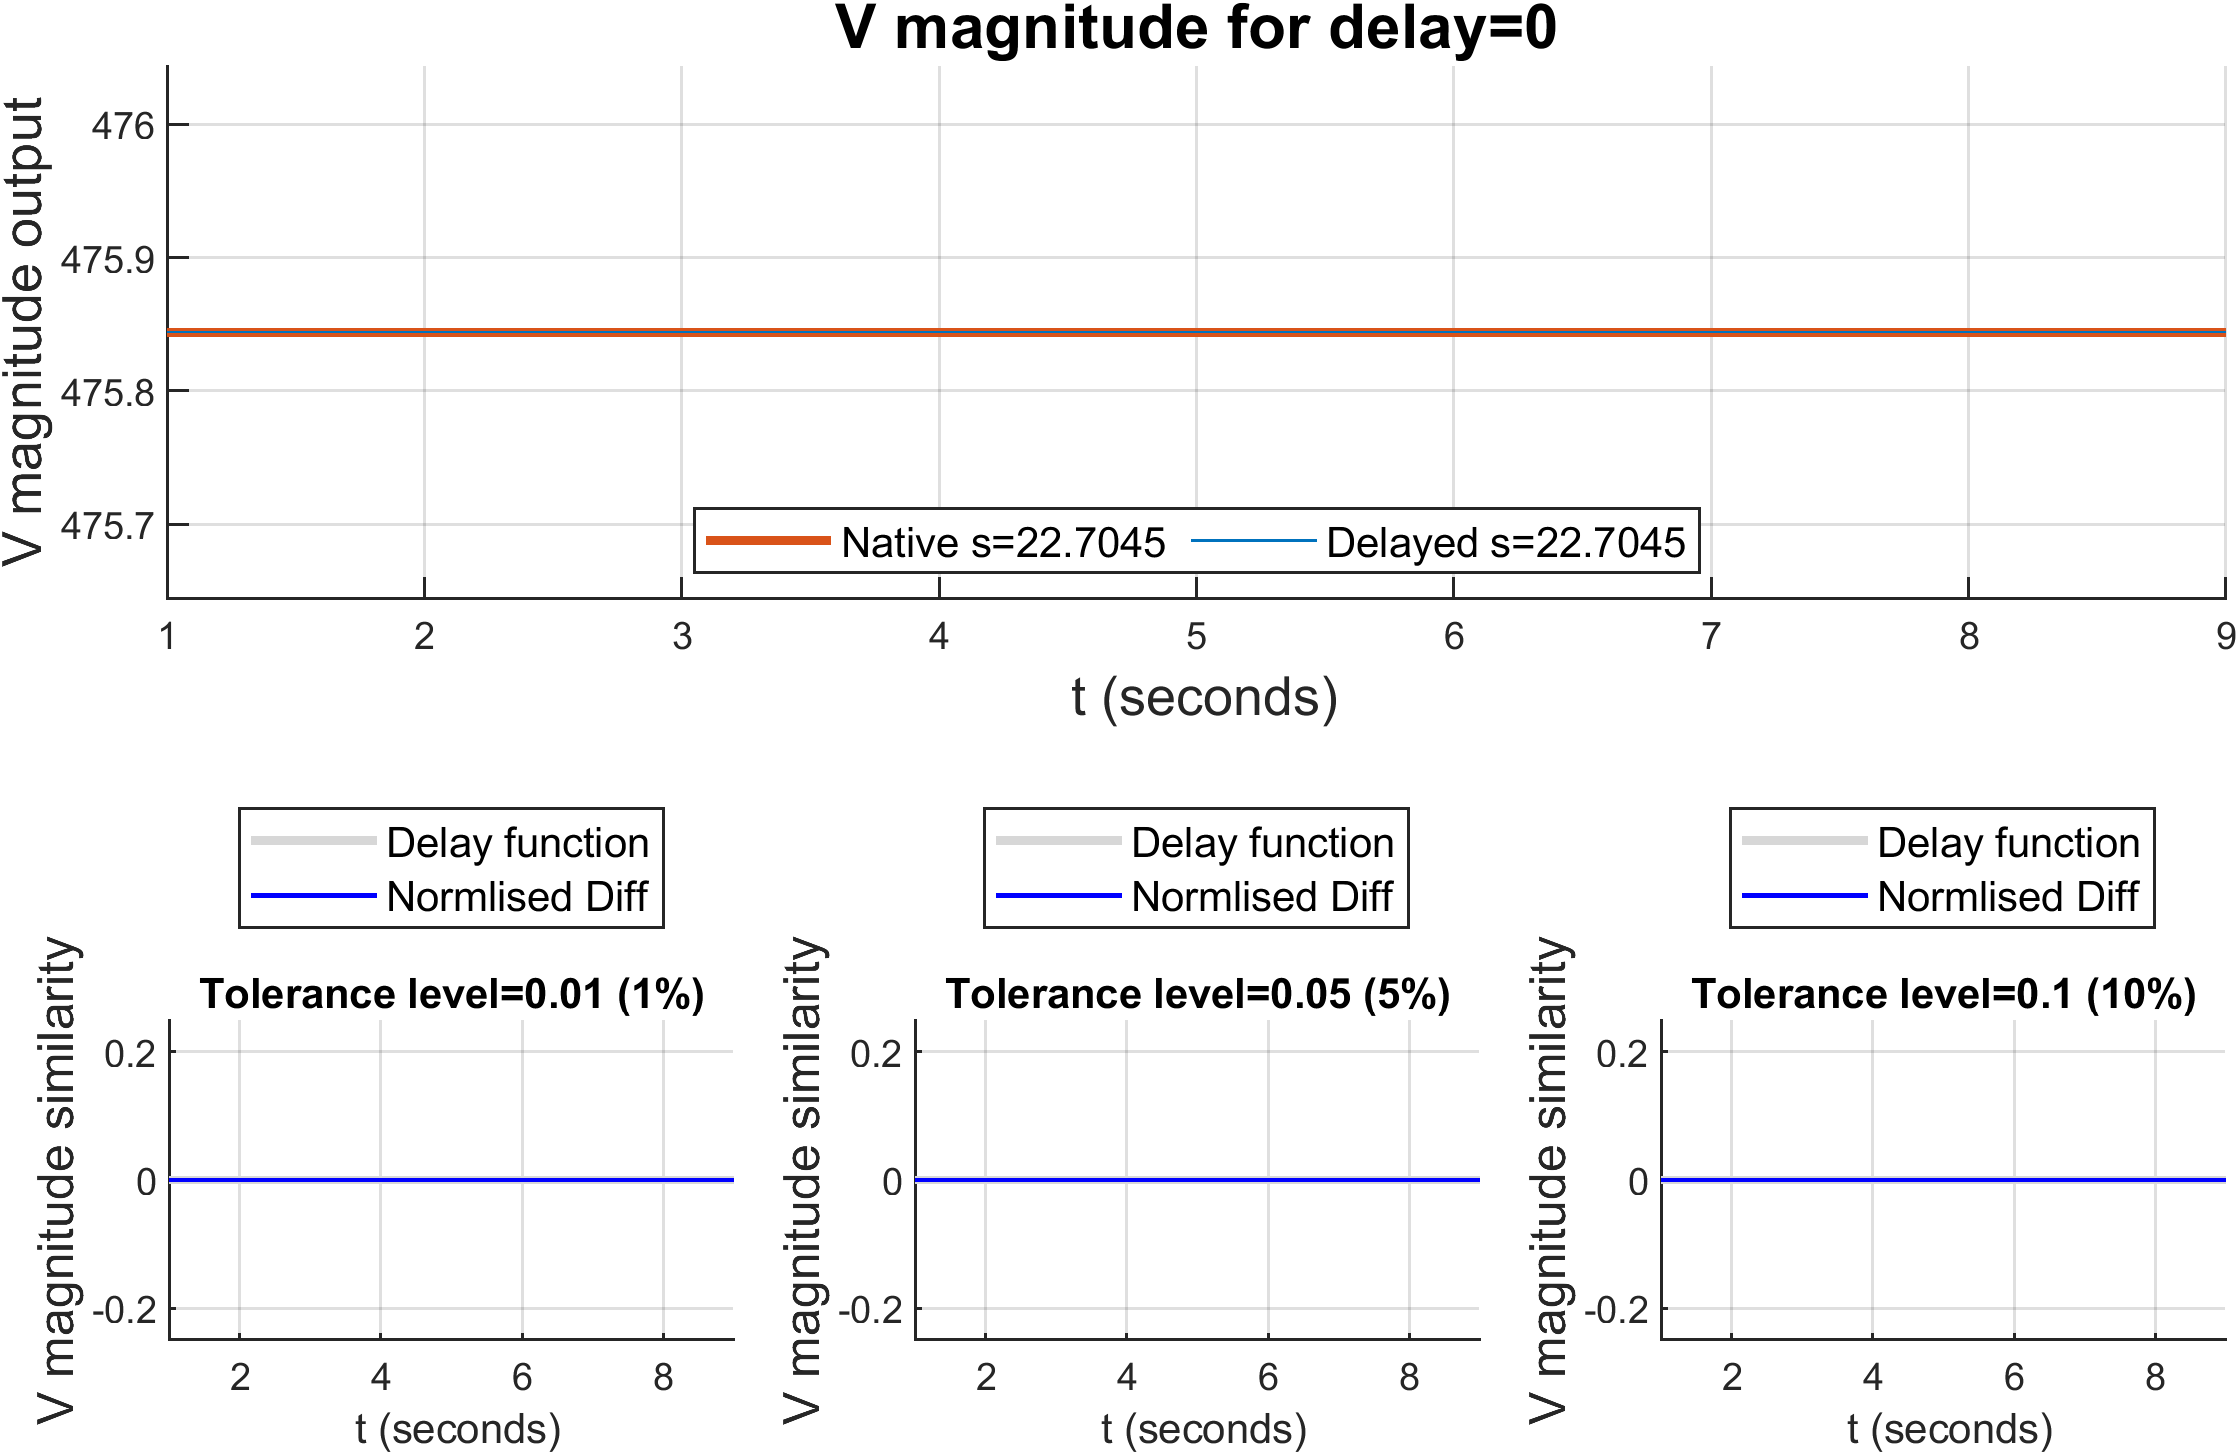
\includegraphics[width=0.95\textwidth]{PMUsim-figures/DelayOf_0/Zero_vMagnitude.png}    
    \label{fig:PMUsim_Zero_vMagnitude}
    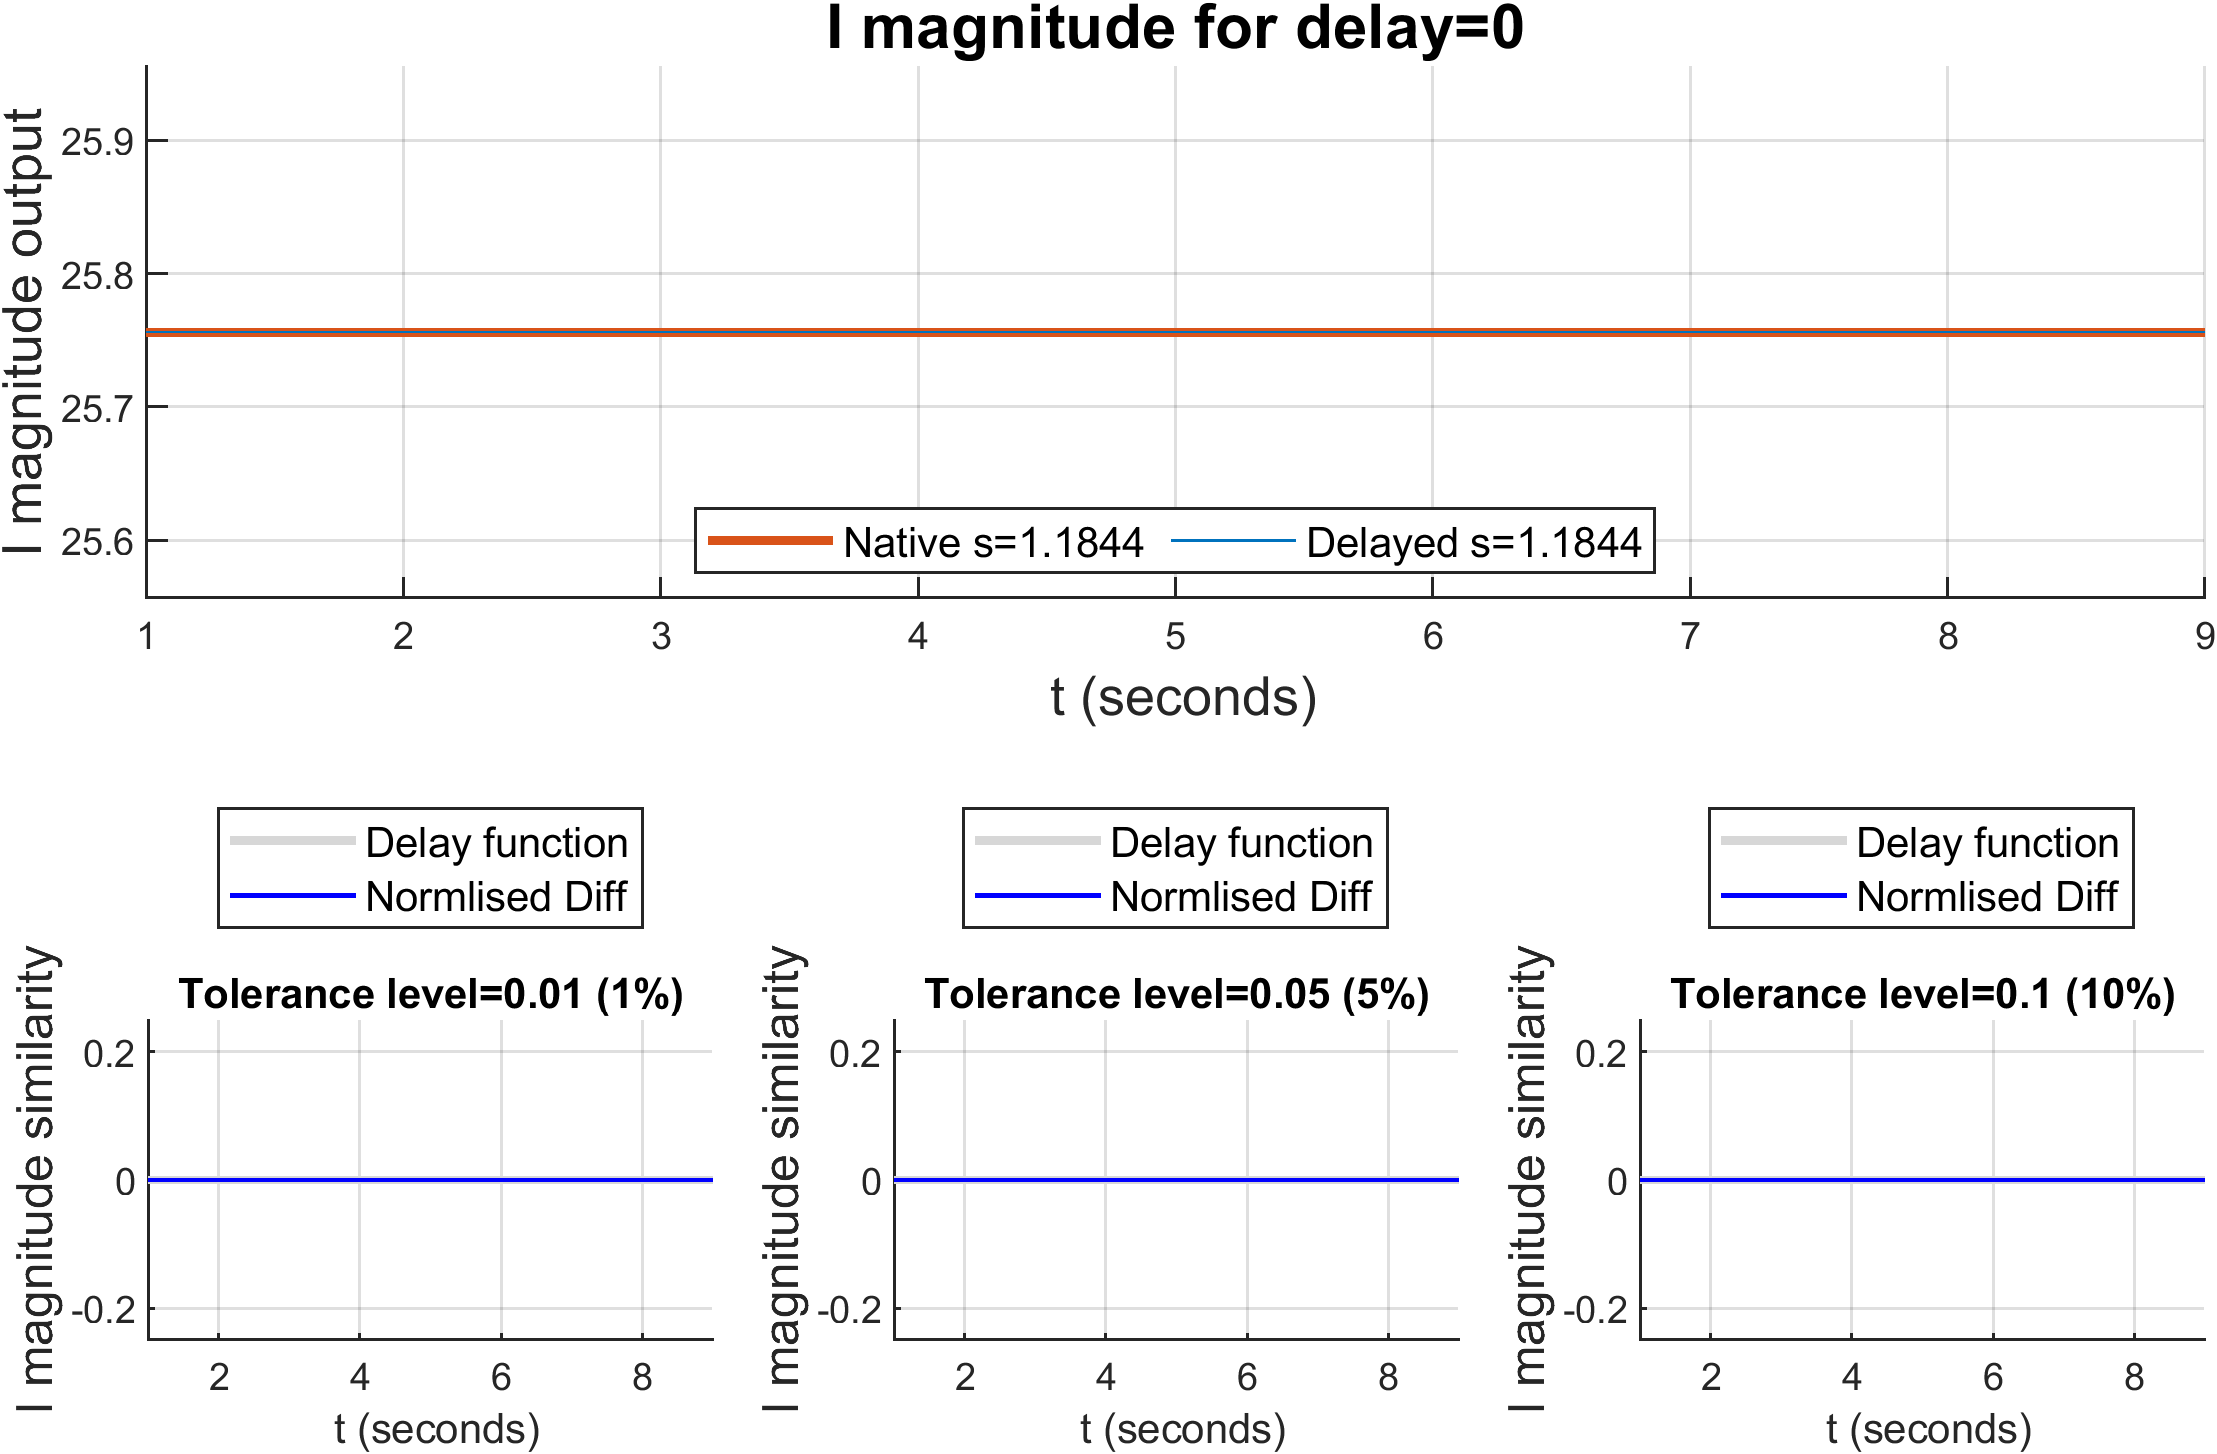
\includegraphics[width=0.95\textwidth]{PMUsim-figures/DelayOf_0/Zero_iMagnitude.png}    
    \caption{Zero Delay Magnitude Output (for the Delay Level of Zero)}
    \label{fig:PMUsim_Zero_Magnitude}
\end{floatingfigure}
\begin{small}
     \tcbox[size=small, standard jigsaw, opacityback=0, boxrule=0pt,halign=justify]{
     Comment on the figure:}{
          \begin{itemize}
         \item      The delayed signal (blue) overlaps the original signal (red), producing a straight line, colored neither red nor blue.
         \item  The blue Normalised diff signal also overlaps the grey delay function.
          \end{itemize} }
\end{small}

\newpage \subsection{Results for Frequency Output}
\begin{floatingfigure}[p]{\textwidth}
    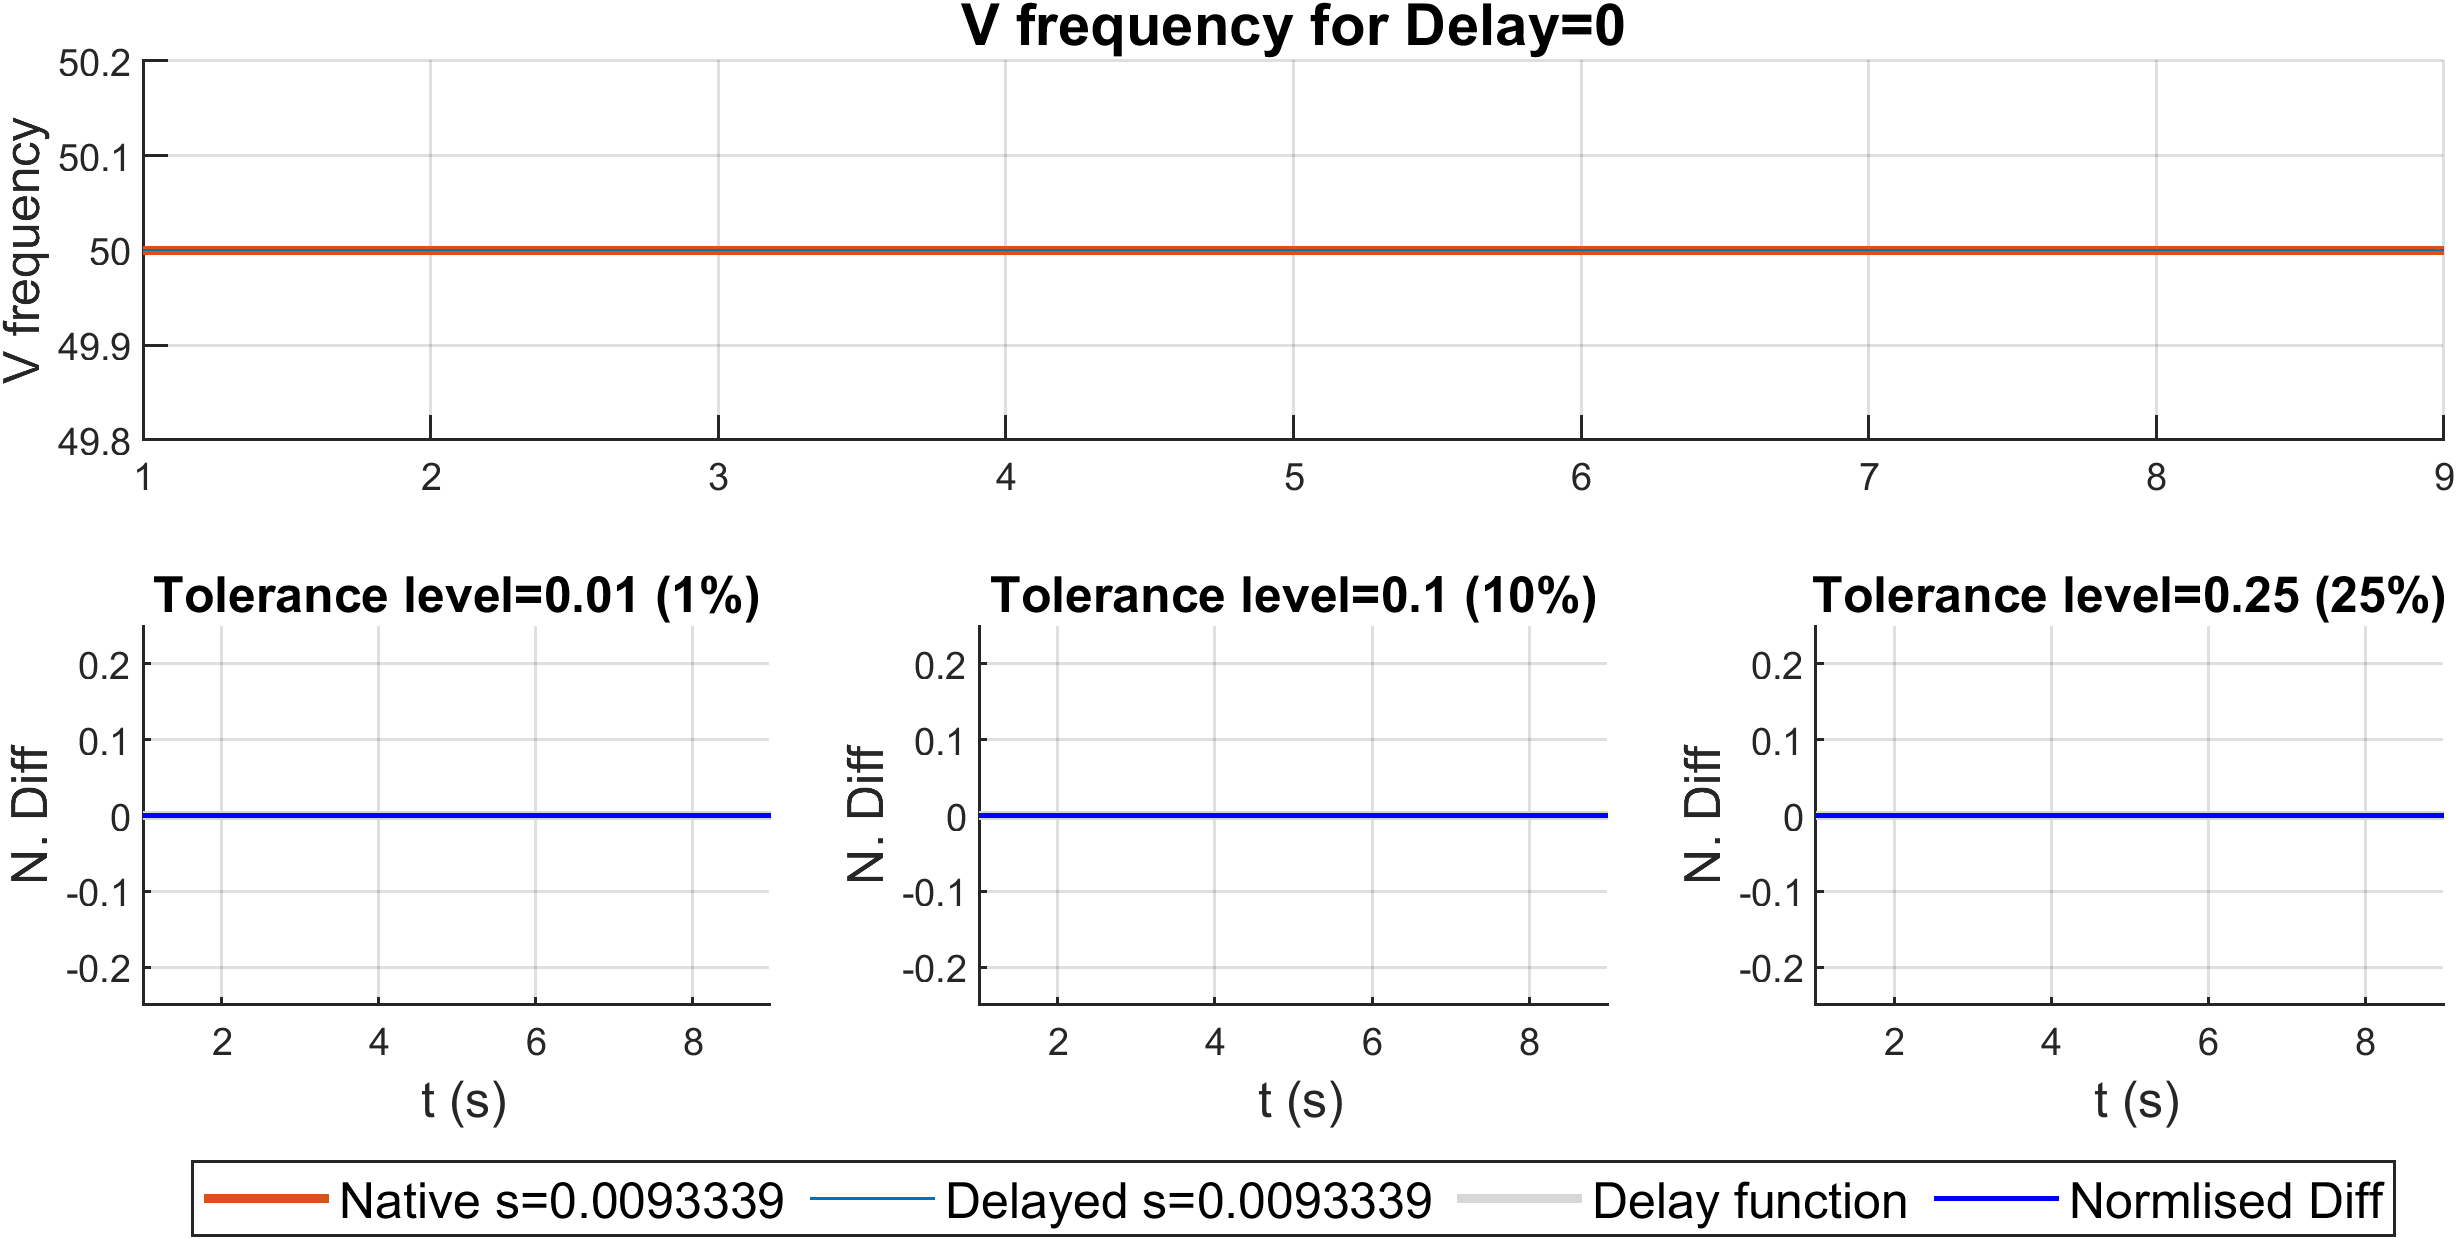
\includegraphics[width=0.95\textwidth]{PMUsim-figures/DelayOf_0/Zero_vFrequency.png}    
    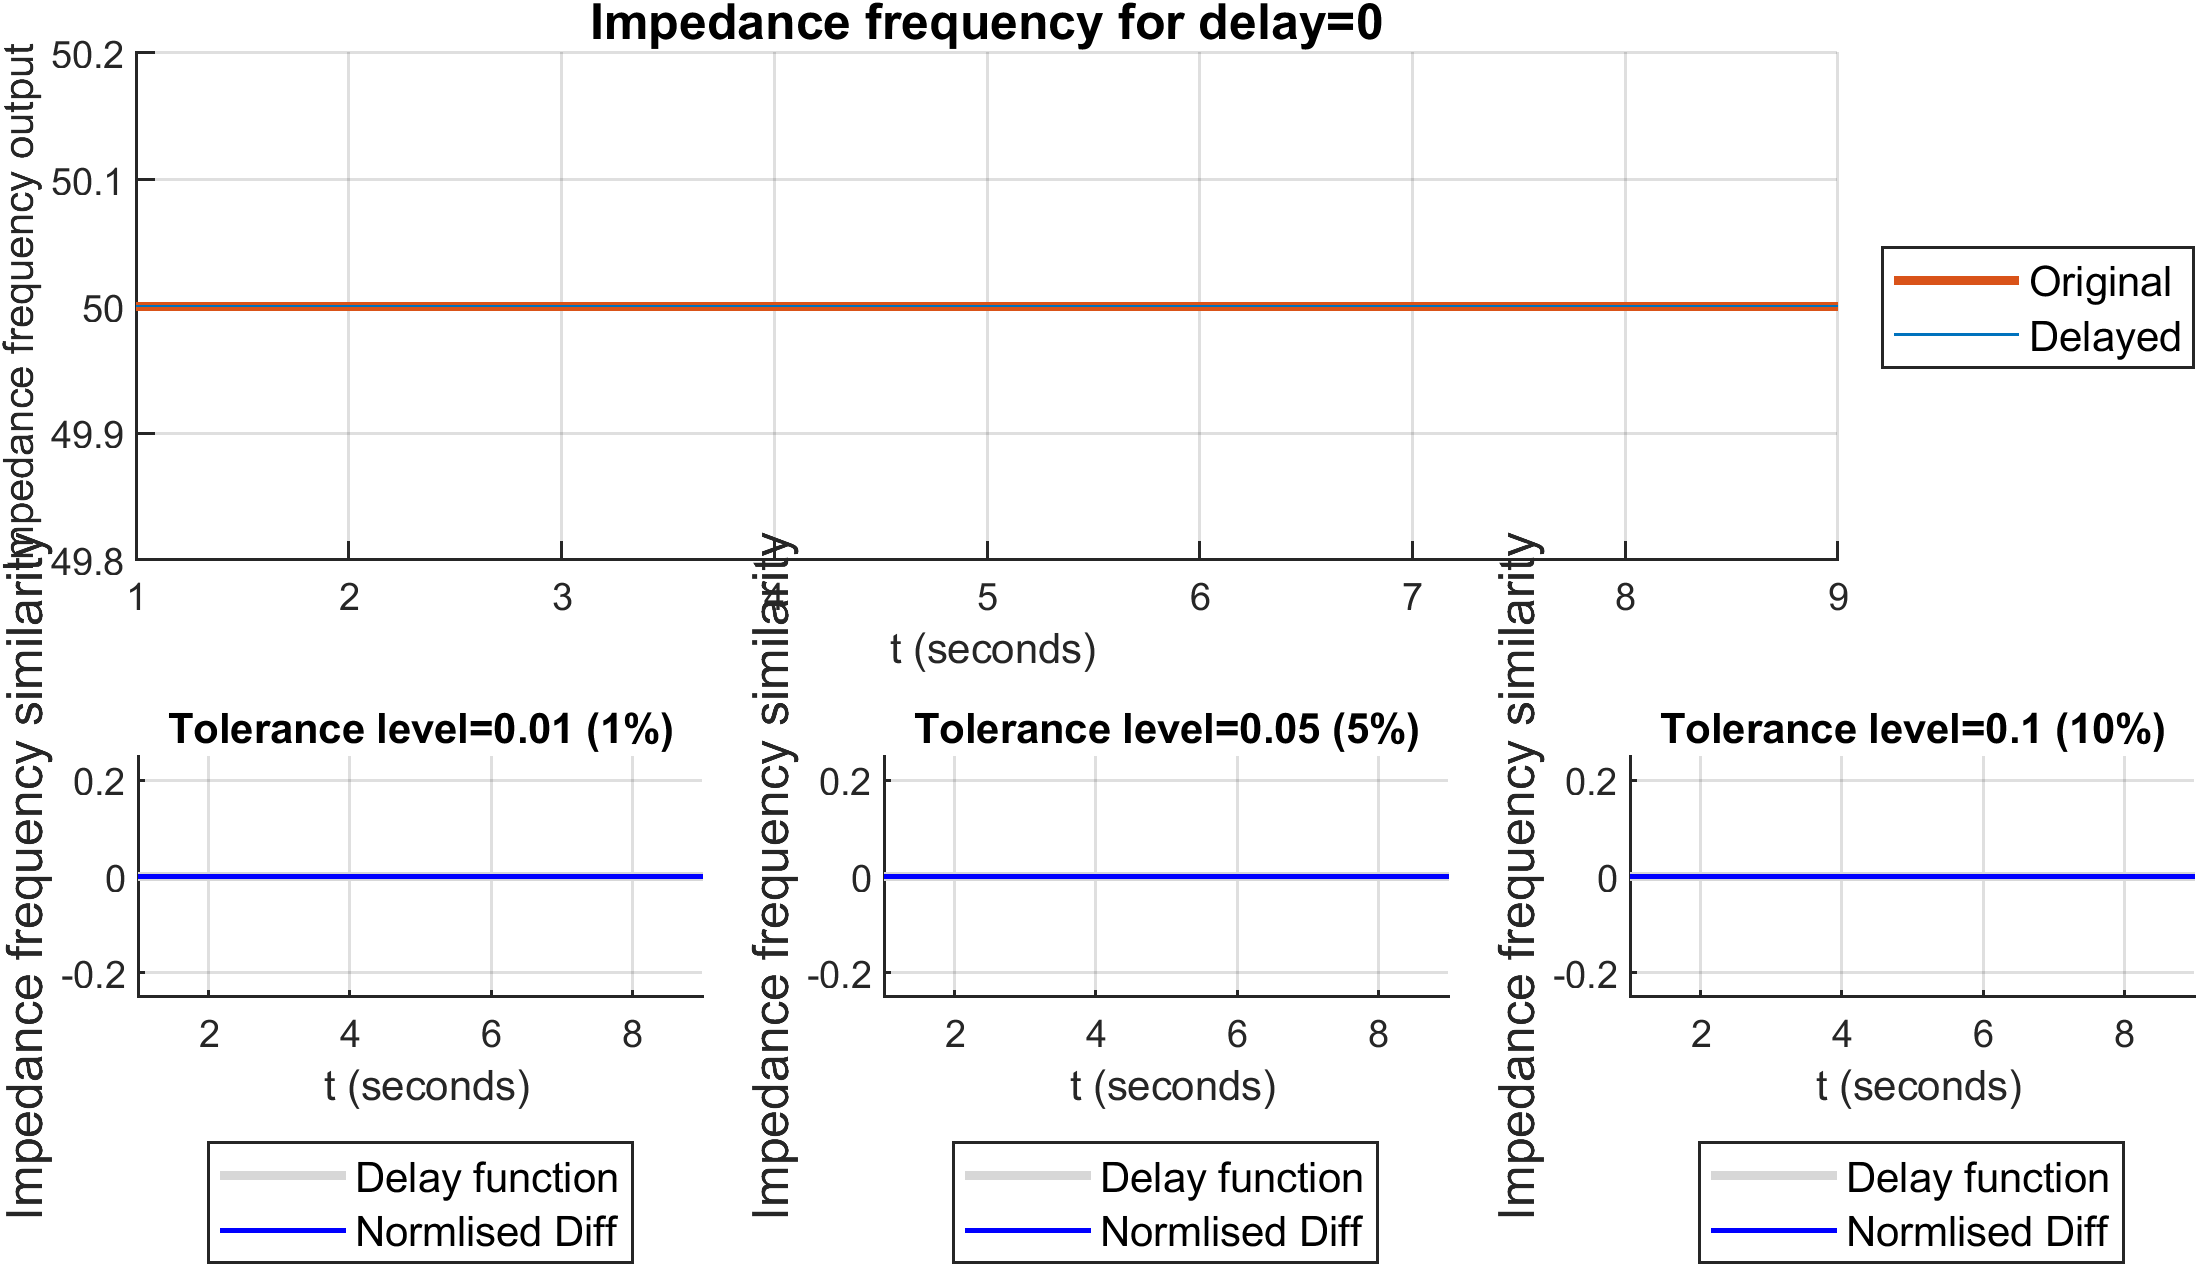
\includegraphics[width=0.95\textwidth]{PMUsim-figures/DelayOf_0/Zero_iFrequency.png}    
    \caption{Zero Delay Frequency Output (for the Delay Level of Zero)}
    \label{fig:PMUsim_Zero_Frequency}
	\end{floatingfigure}

\begin{small}
     \tcbox[size=small, standard jigsaw, opacityback=0, boxrule=0pt,halign=justify]{
     Comment on the figure:}{
          \begin{itemize}
         \item      The delayed signal (blue) overlaps the original signal (red), producing a straight line, colored neither red nor blue.
         \item  The blue Normalised diff signal also overlaps the grey delay function.
          \end{itemize} }
\end{small}

\newpage \subsection{Results for Angle Output}

\begin{floatingfigure}[p]{\textwidth}
    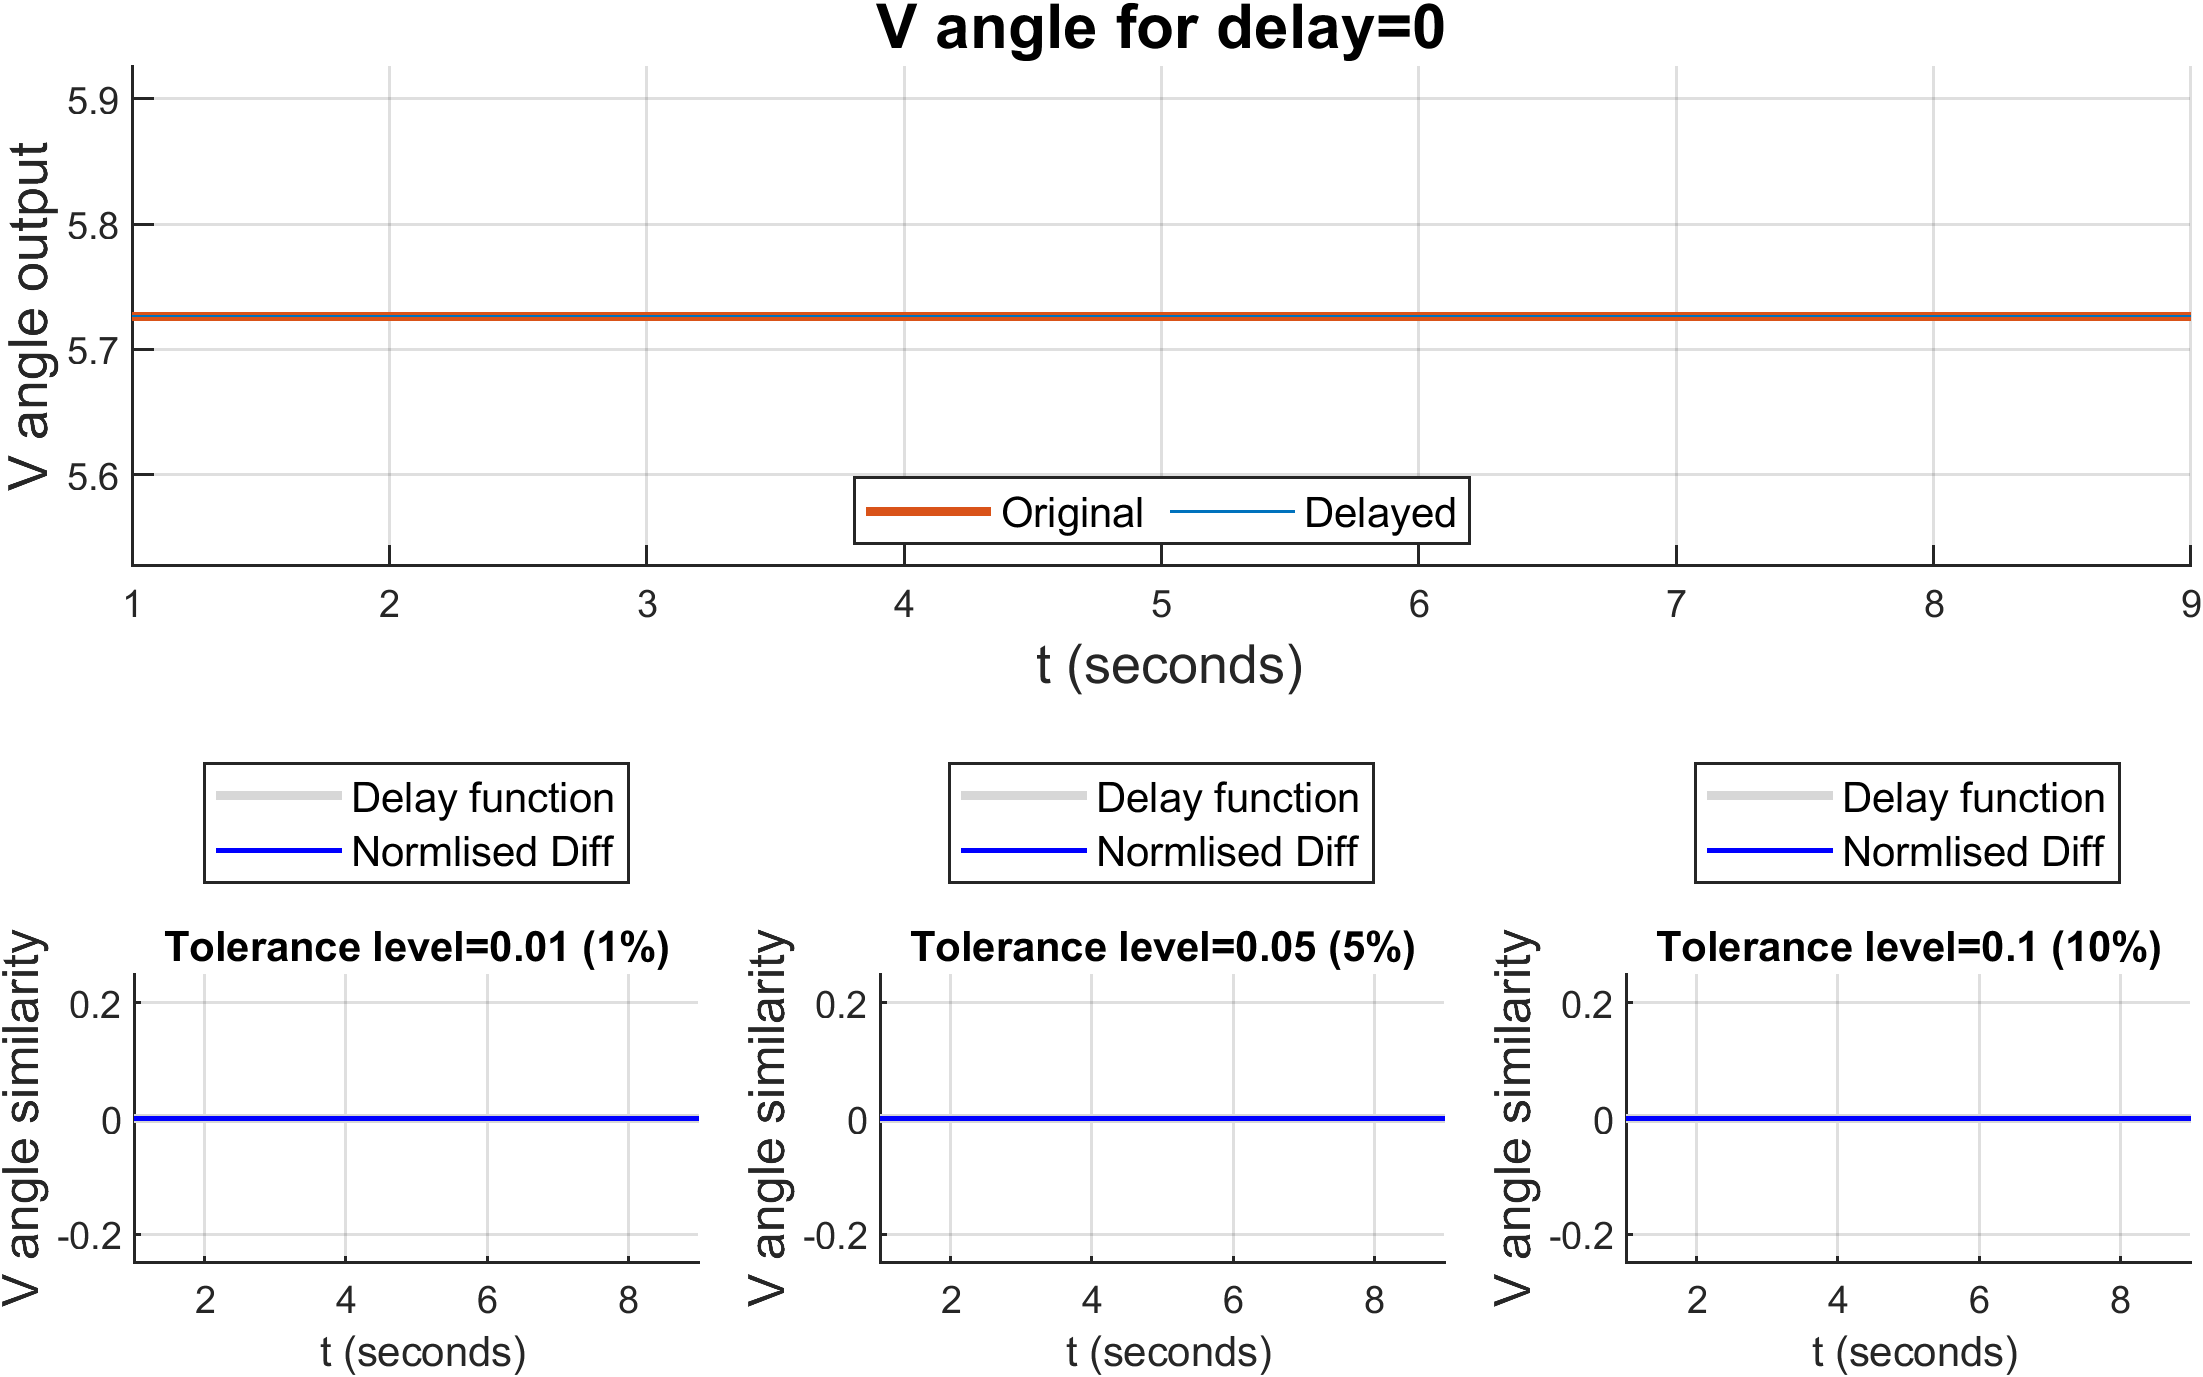
\includegraphics[width=0.95\textwidth]{PMUsim-figures/DelayOf_0/Zero_vAngle.png}    
     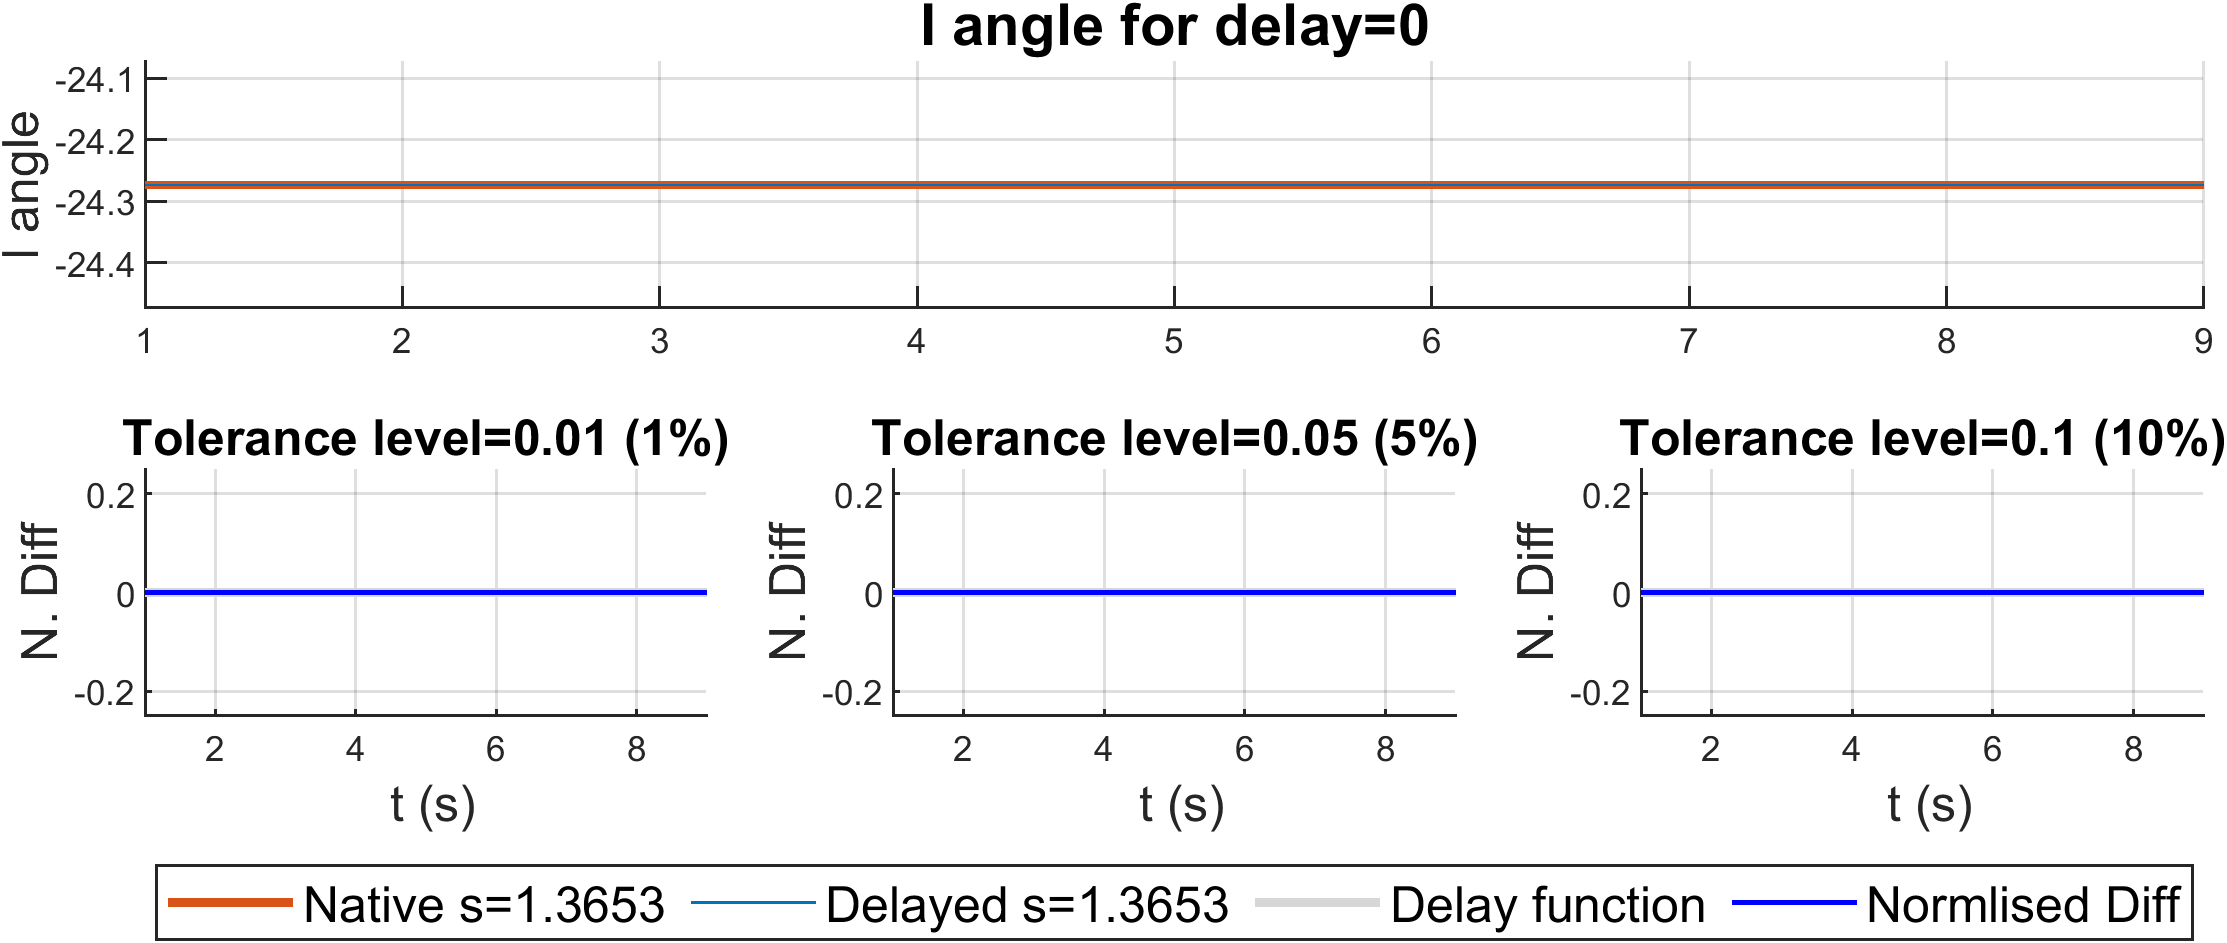
\includegraphics[width=0.95\textwidth]{PMUsim-figures/DelayOf_0/Zero_iAngle.png} 
          \caption{Zero Delay Angle Output (for the Delay Level of Zero)}

              \label{fig:PMUsim_Zero_Angle}
\end{floatingfigure}
\begin{small}
      \tcbox[size=small, standard jigsaw, opacityback=0, boxrule=0pt,halign=justify]{
     Comment on the figure:}{
          \begin{itemize}
         \item      The delayed signal (blue) overlaps the original signal (red), producing a straight line, colored neither red nor blue.
         \item  The blue Normalised diff signal also overlaps the grey delay function.
          \end{itemize} }
\end{small}

\section{Instant Delay Functions}
\newpage \subsection{Delay Level of One}
\textbf{Results for Magnitude Output}
\begin{floatingfigure}[p]{\textwidth}[bp]
    \caption{Instant Delay Magnitude Output for the Delay Level of One}
    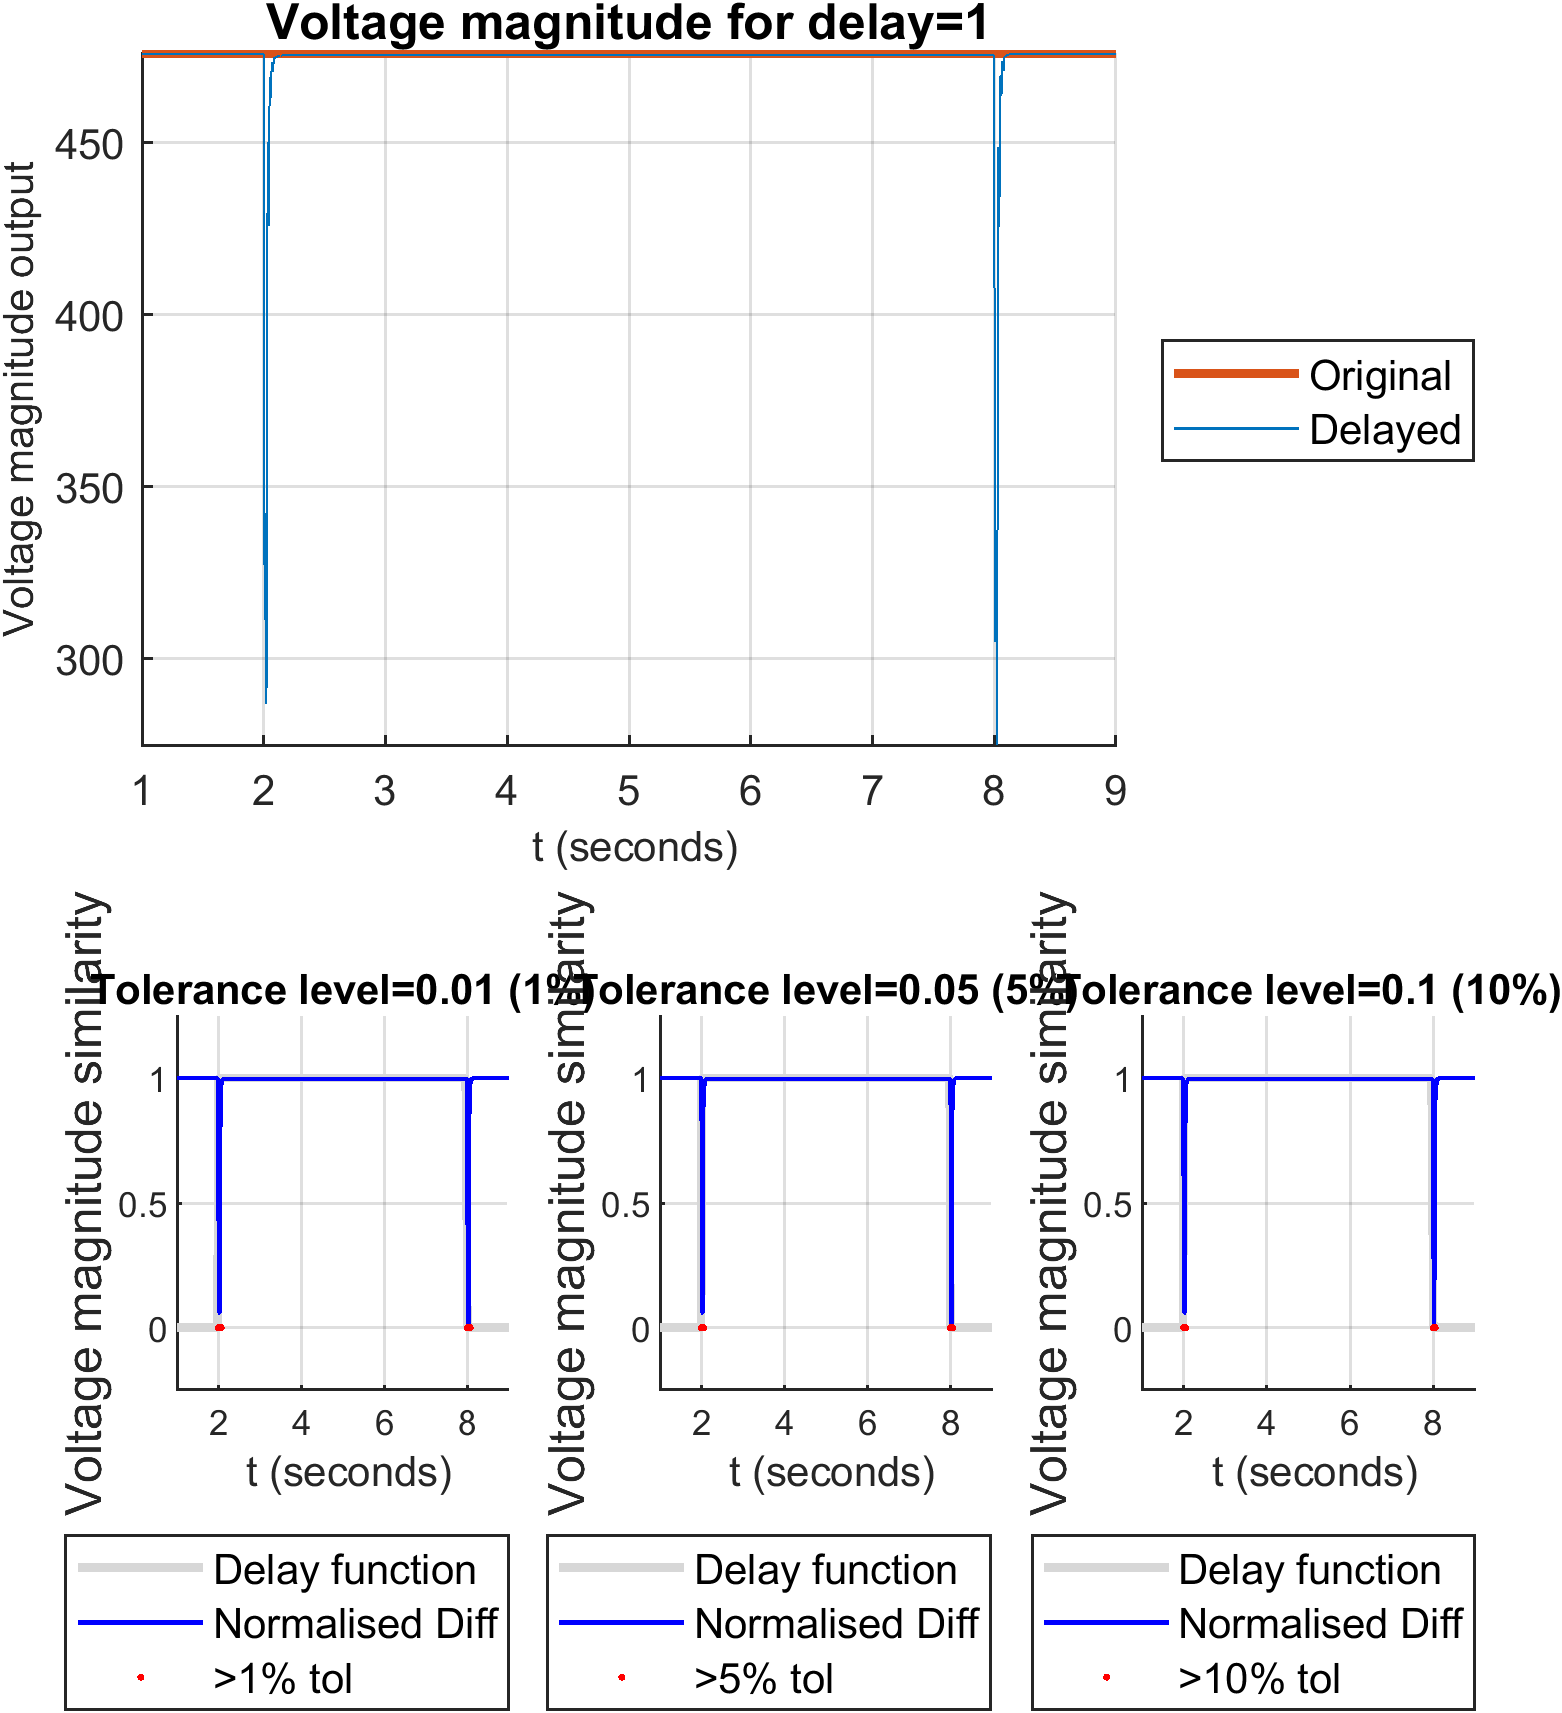
\includegraphics[width=0.95\textwidth]{PMUsim-figures/DelayOf_1/Instant_vMagnitude.png}    
      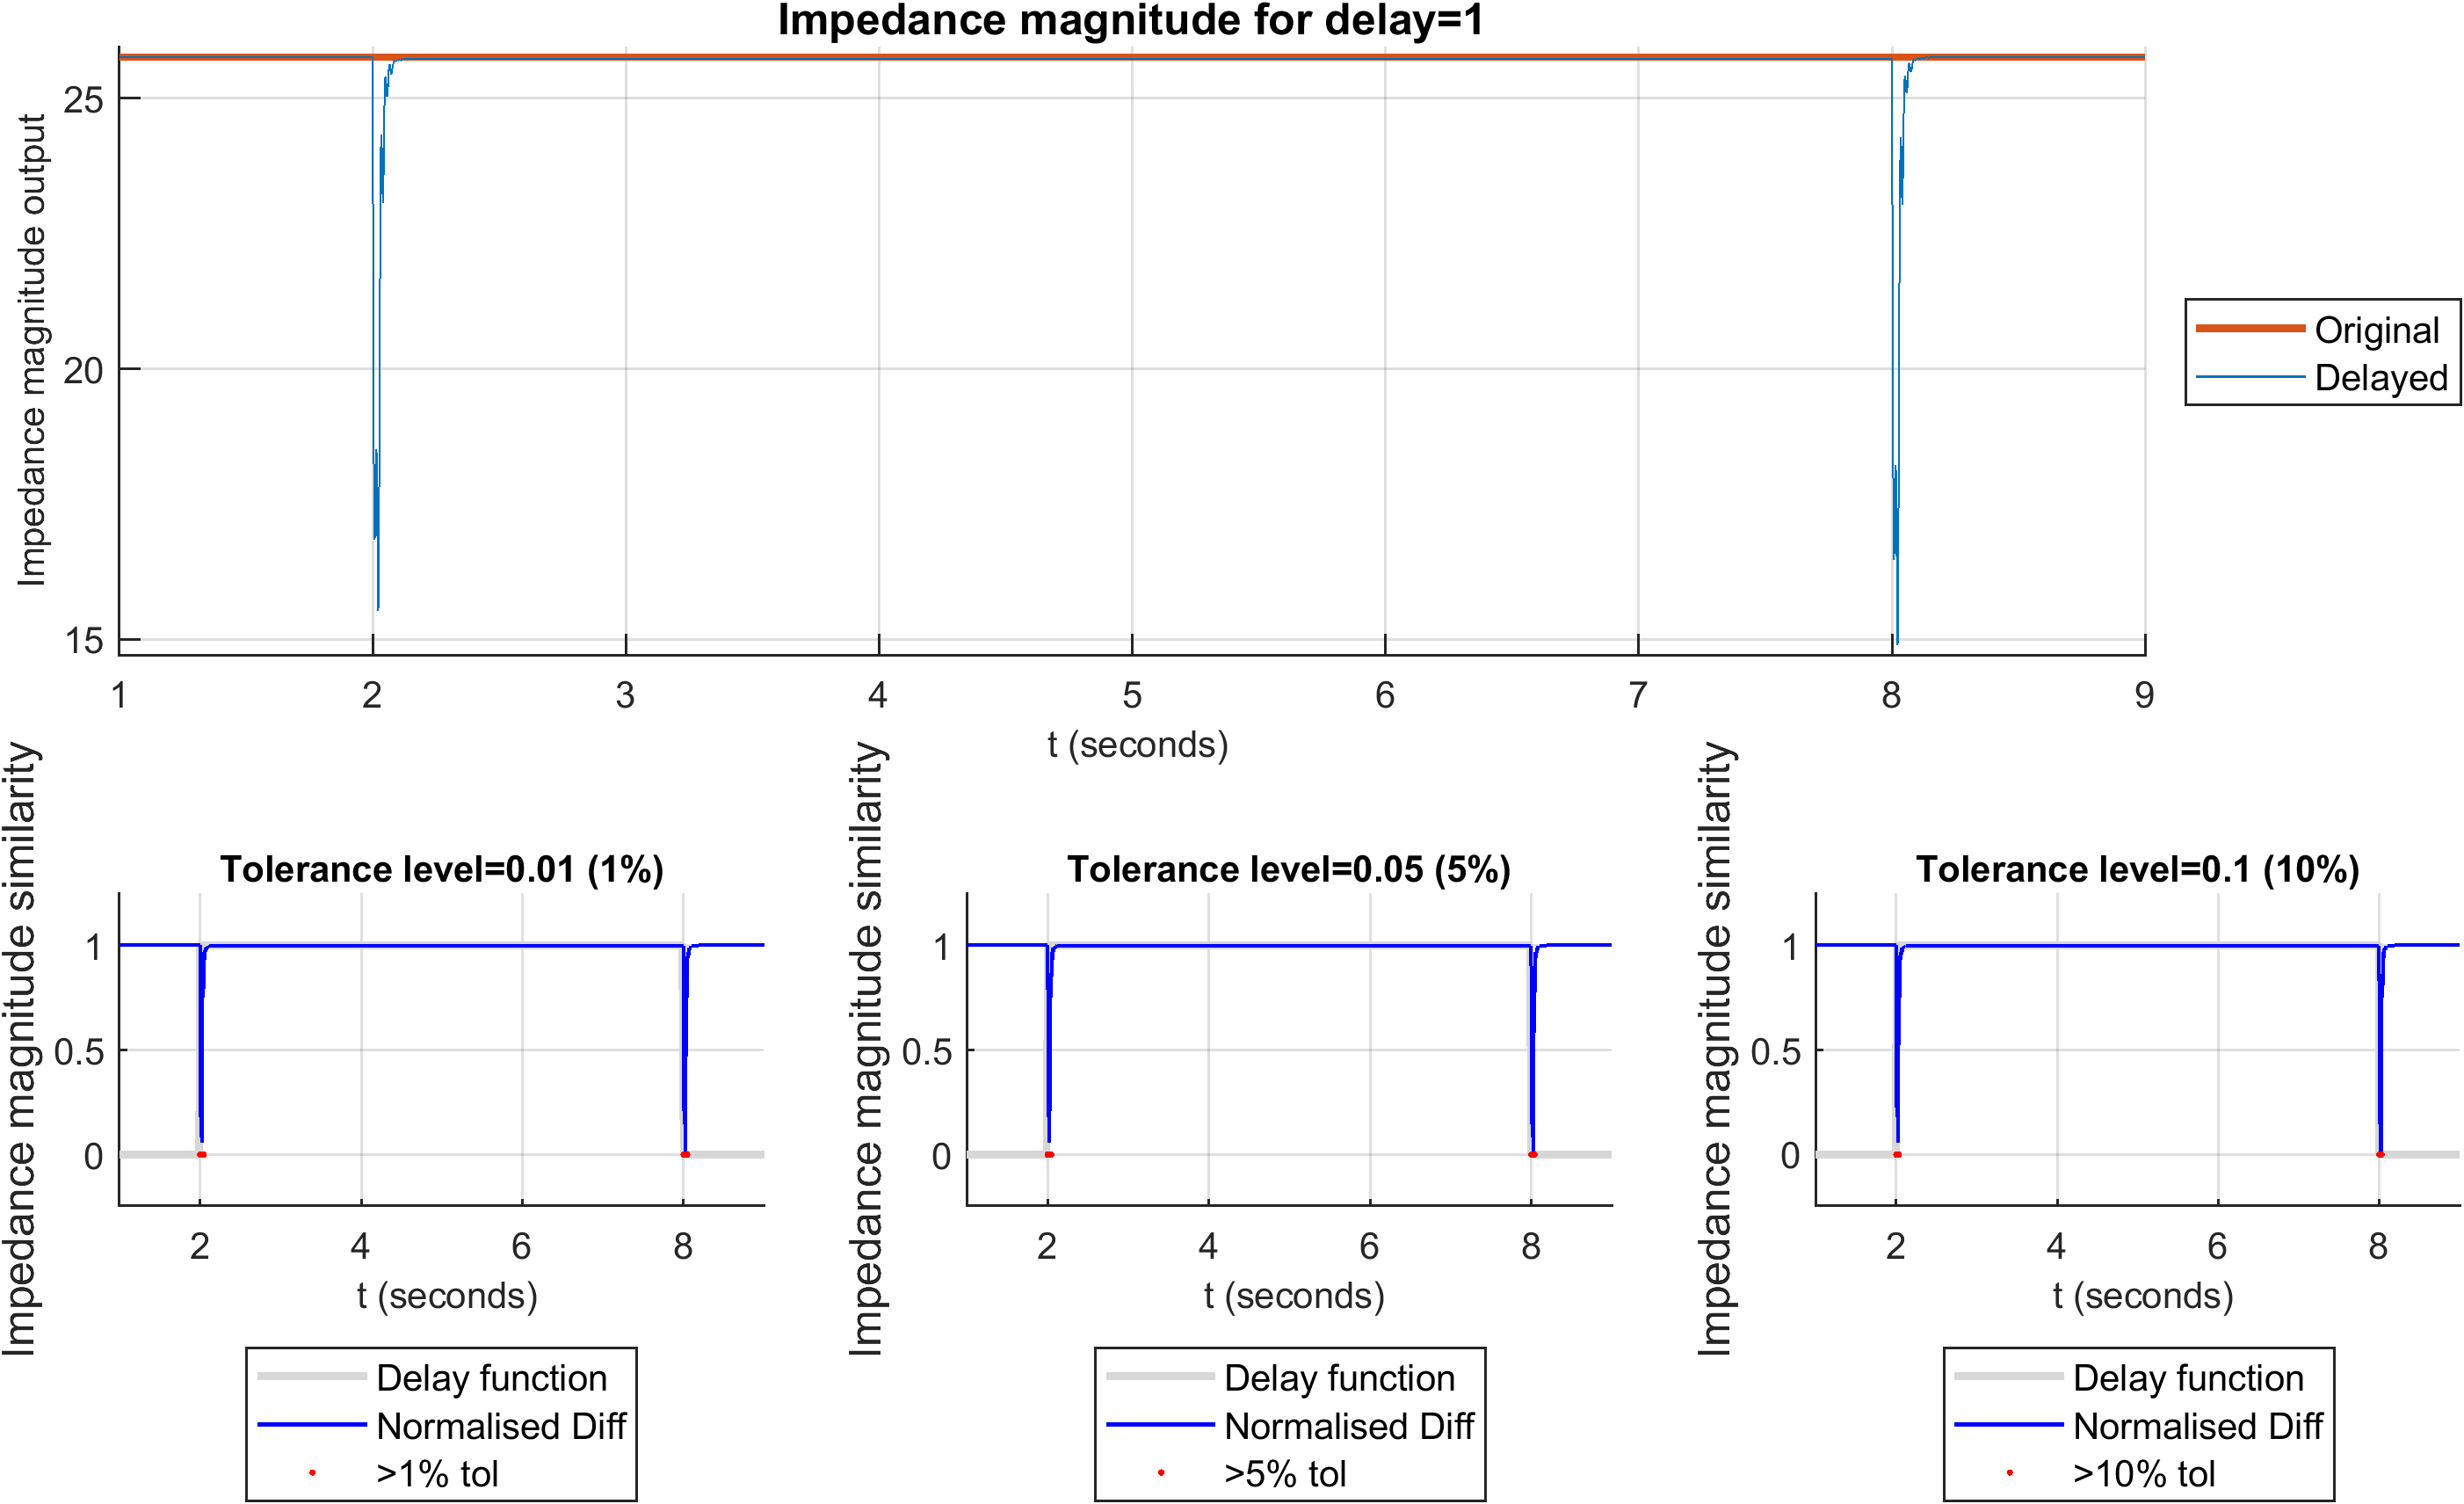
\includegraphics[width=0.95\textwidth]{PMUsim-figures/DelayOf_1/Instant_iMagnitude.png}      
    \label{fig:PMUsim_One_Magnitude}
\end{floatingfigure}
    \begin{small}
     \tcbox[size=small, standard jigsaw, opacityback=0, boxrule=0pt,halign=justify]{
           comment on the figure:}{\begin{itemize}          \item       \end{itemize} }
     \end{small}

\newpage \textbf{Results for Frequency Output}
\begin{floatingfigure}[p]{\textwidth}[bp]
    \caption{Instant Delay Frequency Output for the Delay Level of One}
    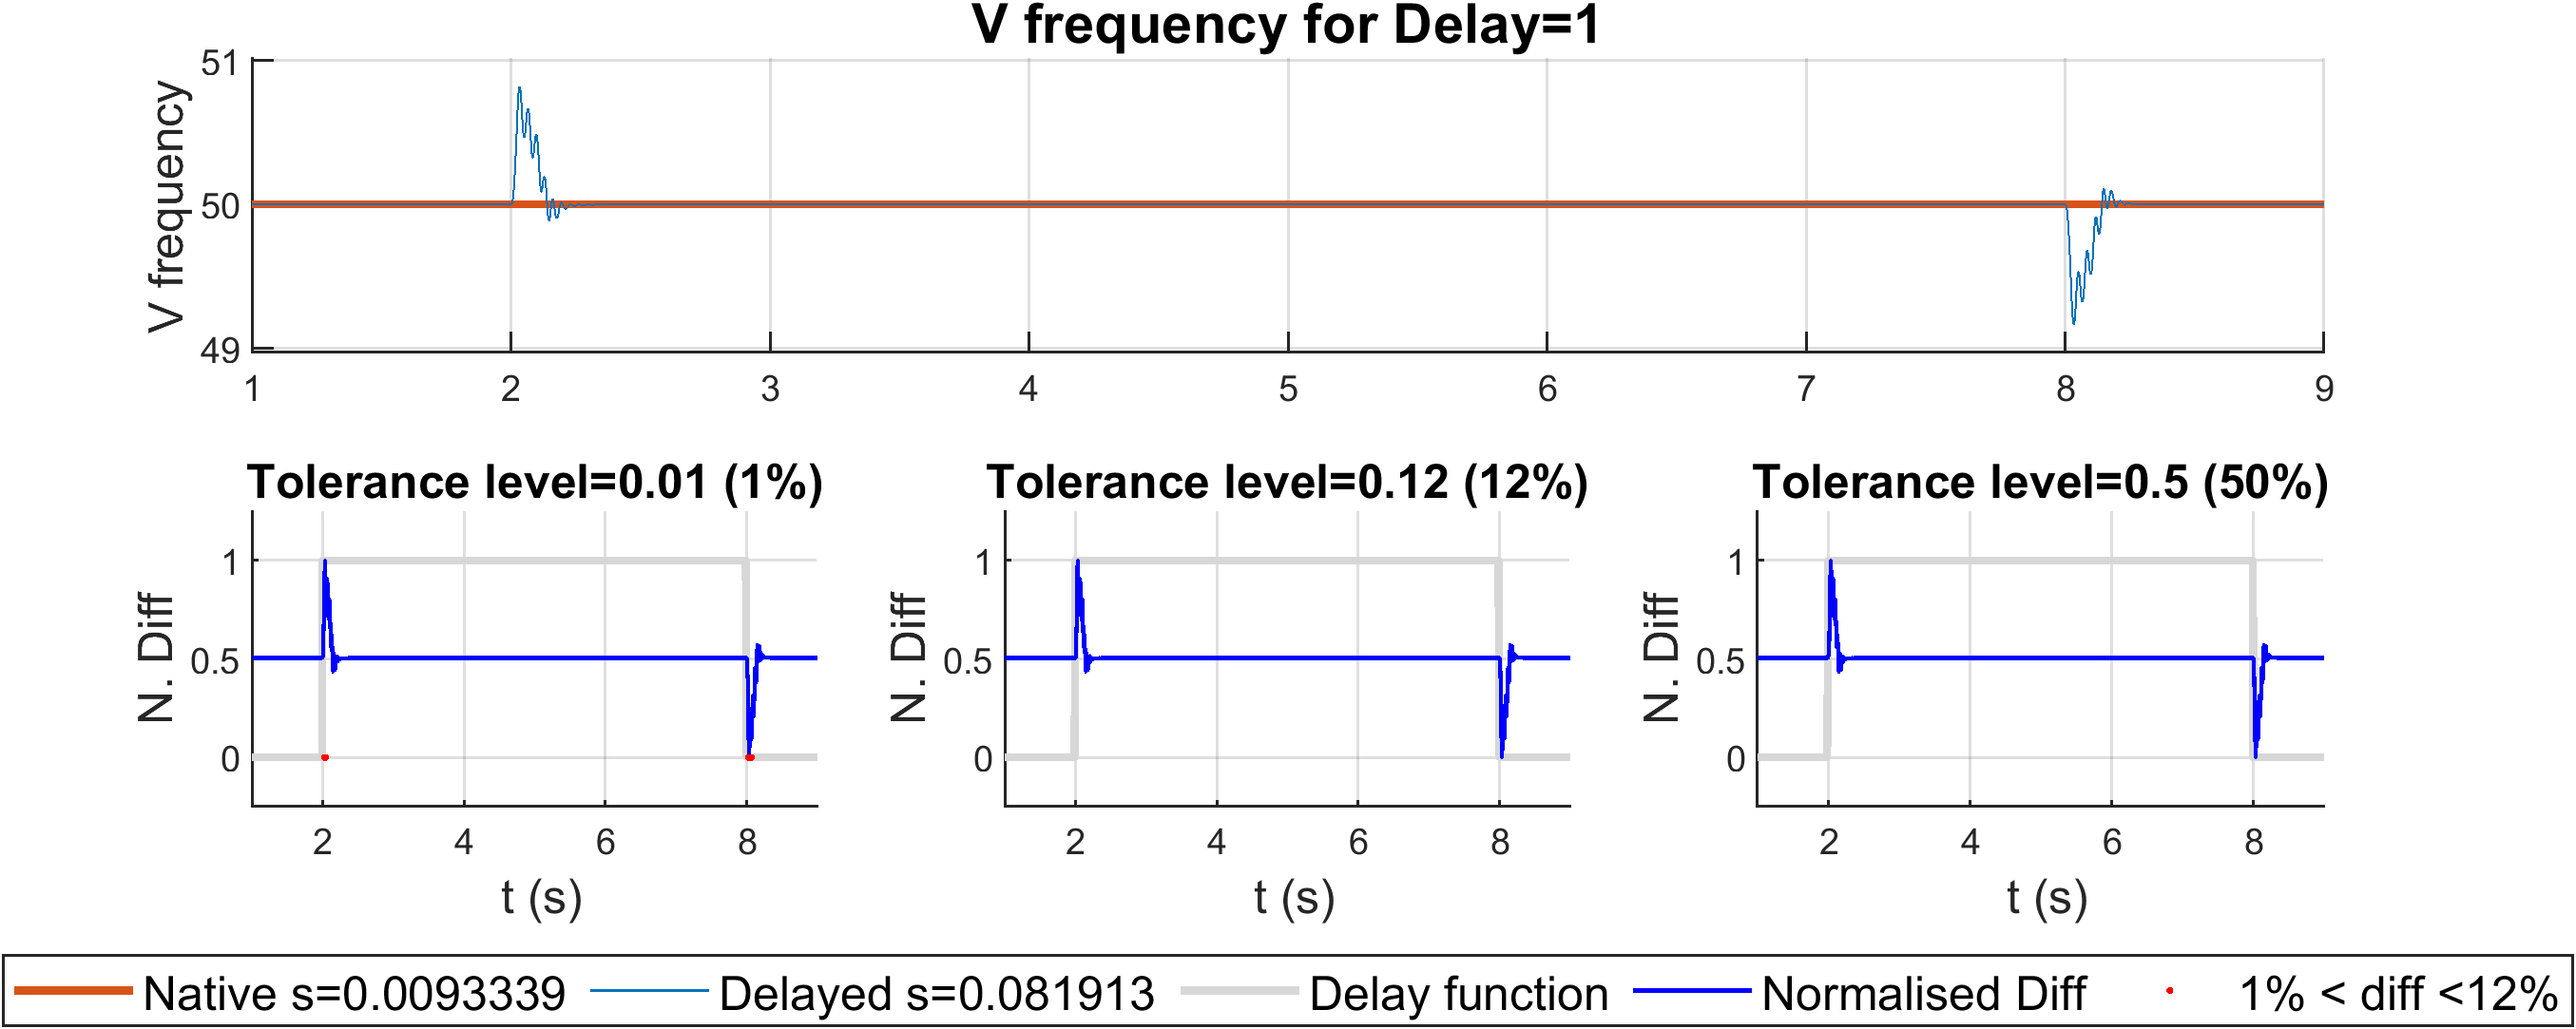
\includegraphics[width=0.95\textwidth]{PMUsim-figures/DelayOf_1/Instant_vFrequency.png}    
  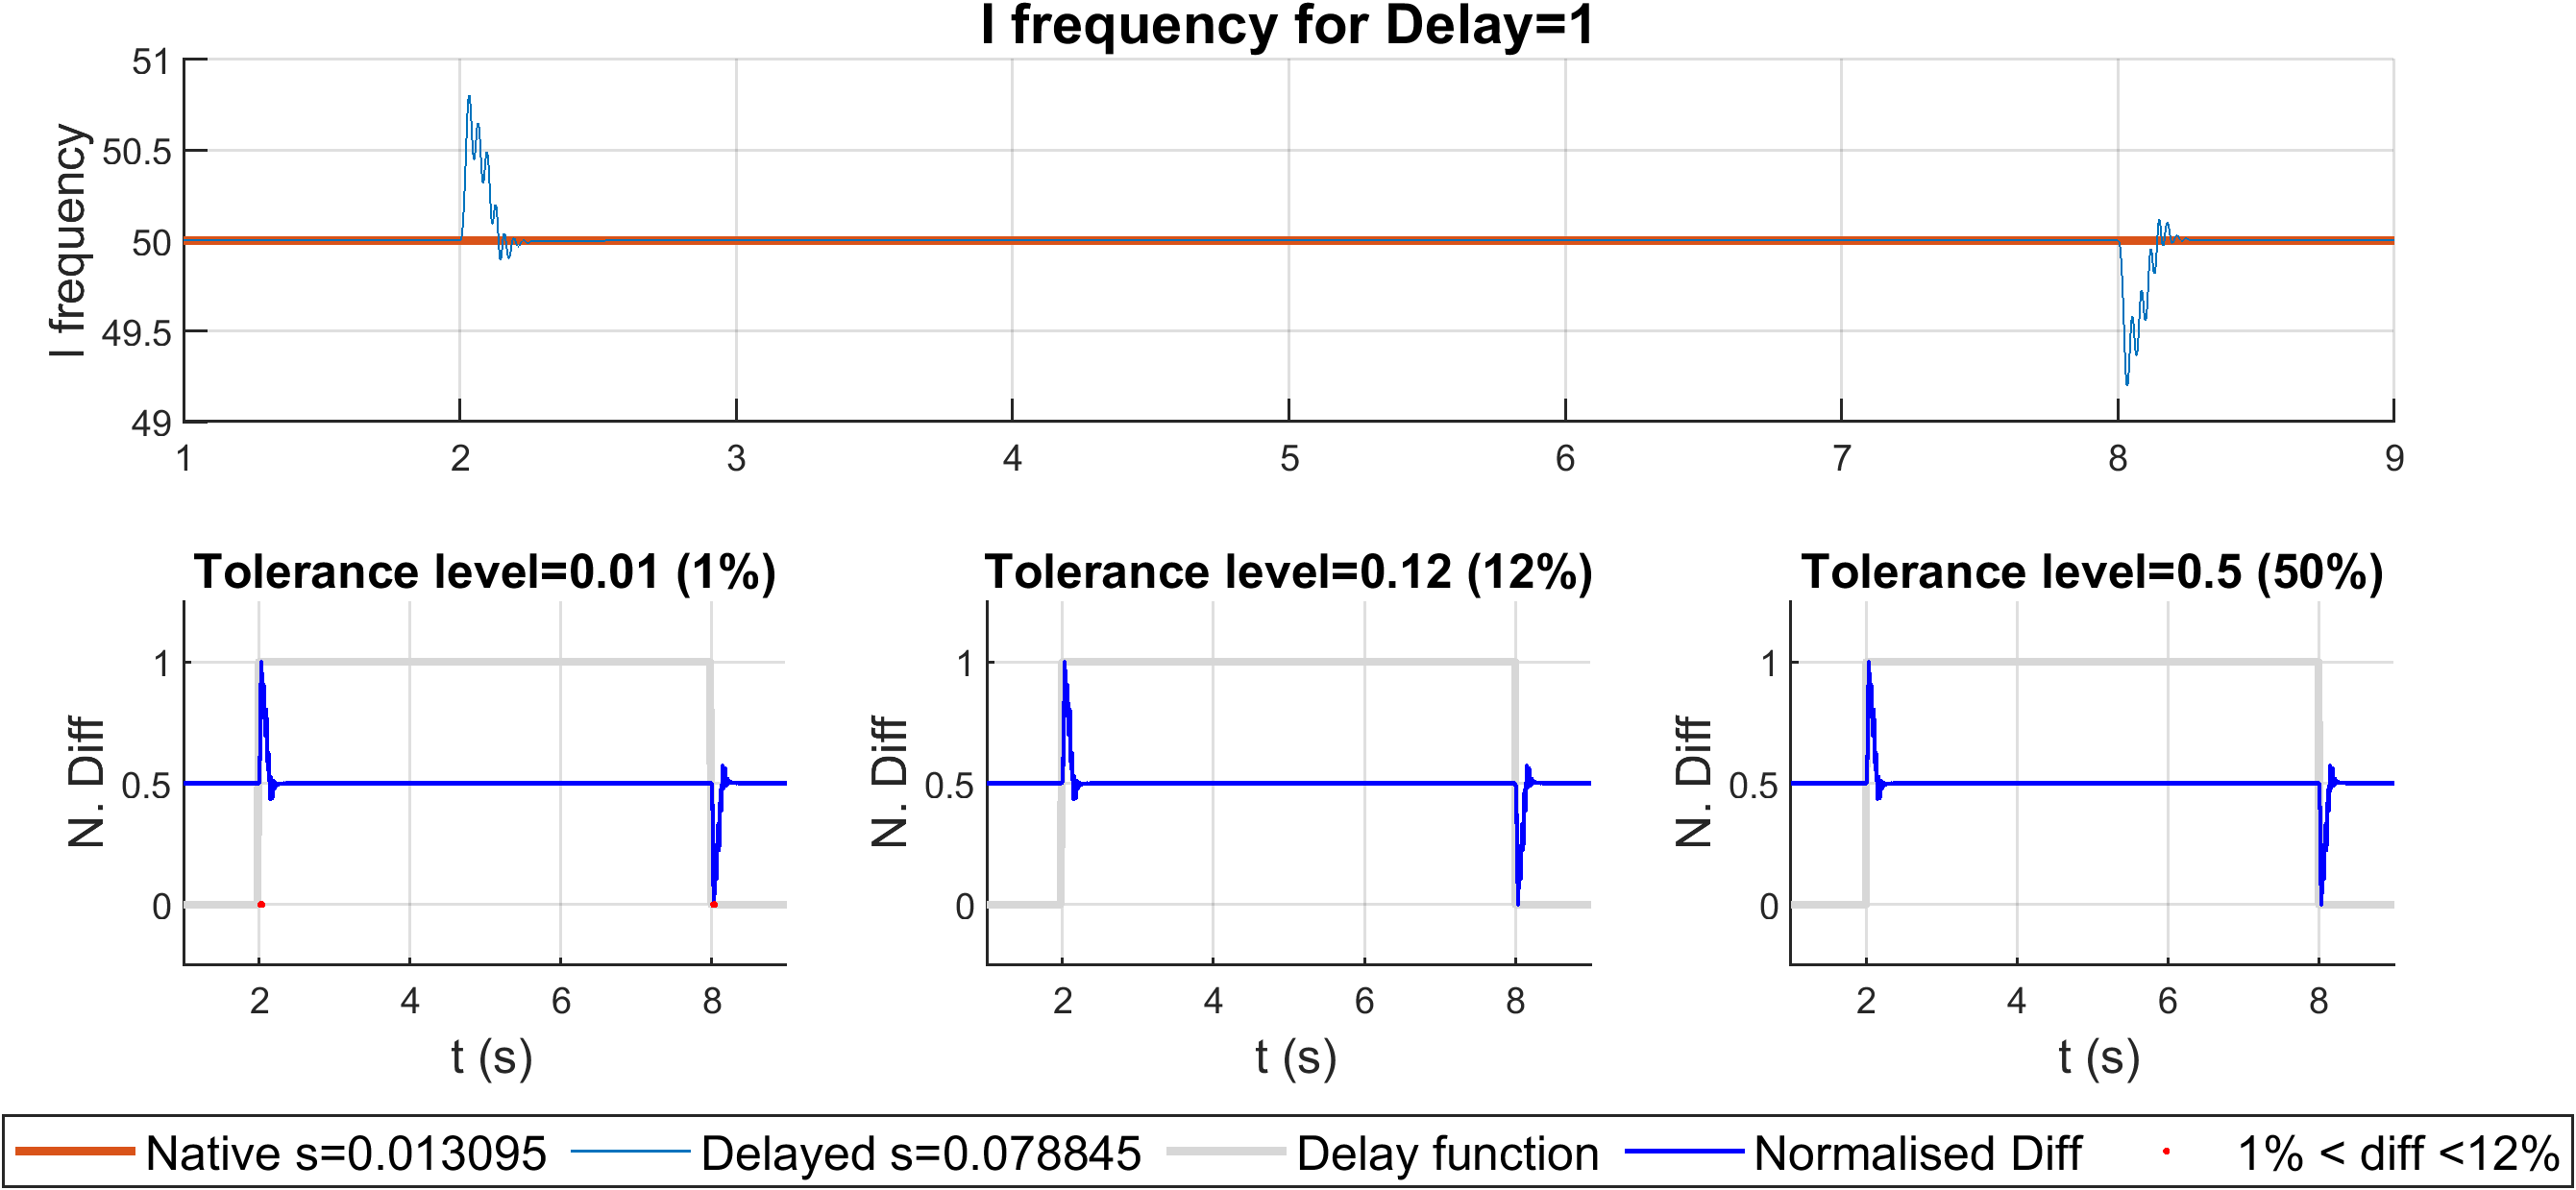
\includegraphics[width=0.95\textwidth]{PMUsim-figures/DelayOf_1/Instant_iFrequency.png}    
    \label{fig:PMUsim_One_Frequency}
\end{floatingfigure}
        \begin{small}
     \tcbox[size=small, standard jigsaw, opacityback=0, boxrule=0pt,halign=justify]{
     Comment on the figure:}{
     \begin{itemize}
         \item 
     \end{itemize} }
     \end{small}

\newpage \textbf{Results for Angle Output}
\begin{floatingfigure}[p]{\textwidth}
    \caption{Instant Delay Angle Output for the Delay Level of One}
    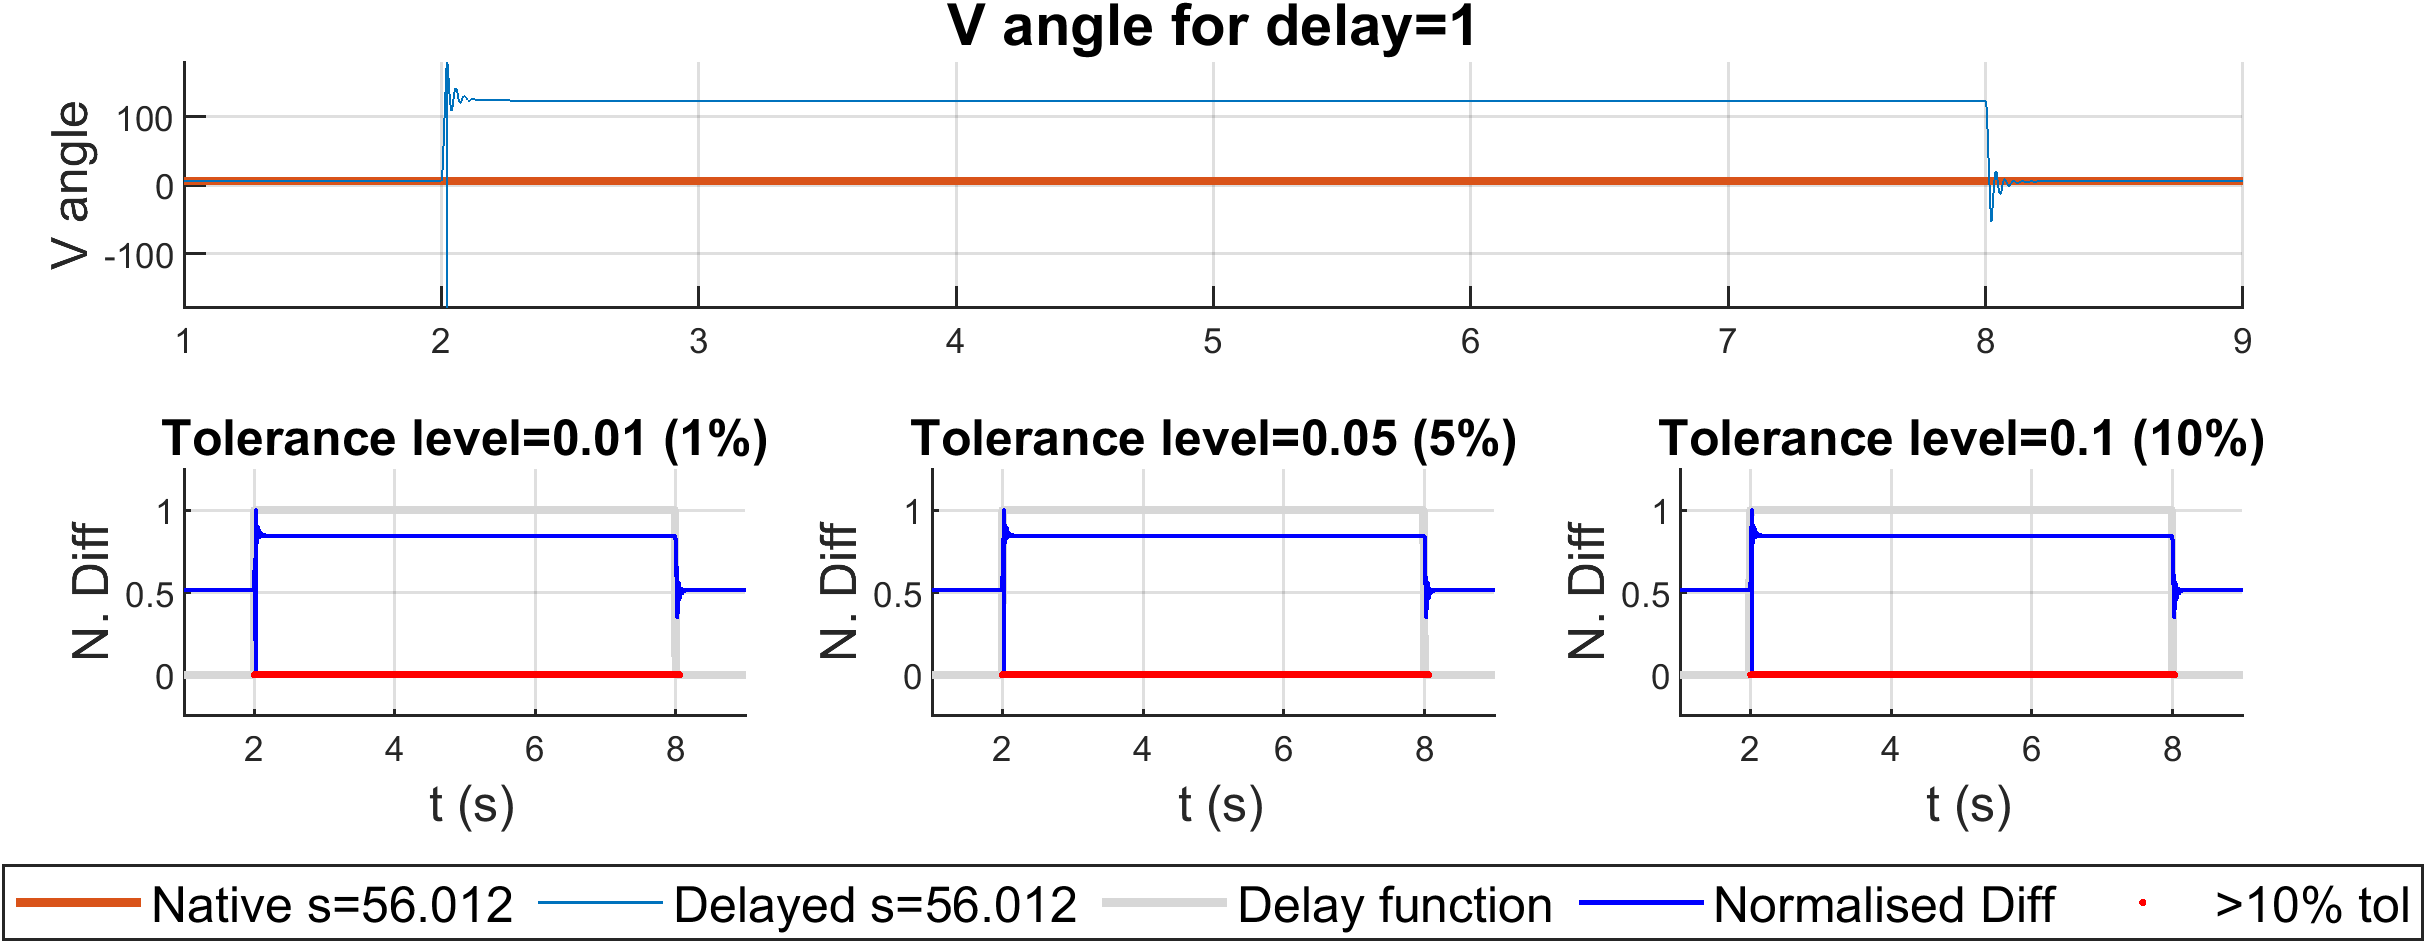
\includegraphics[width=0.95\textwidth]{PMUsim-figures/DelayOf_1/Instant_vAngle.png}    
    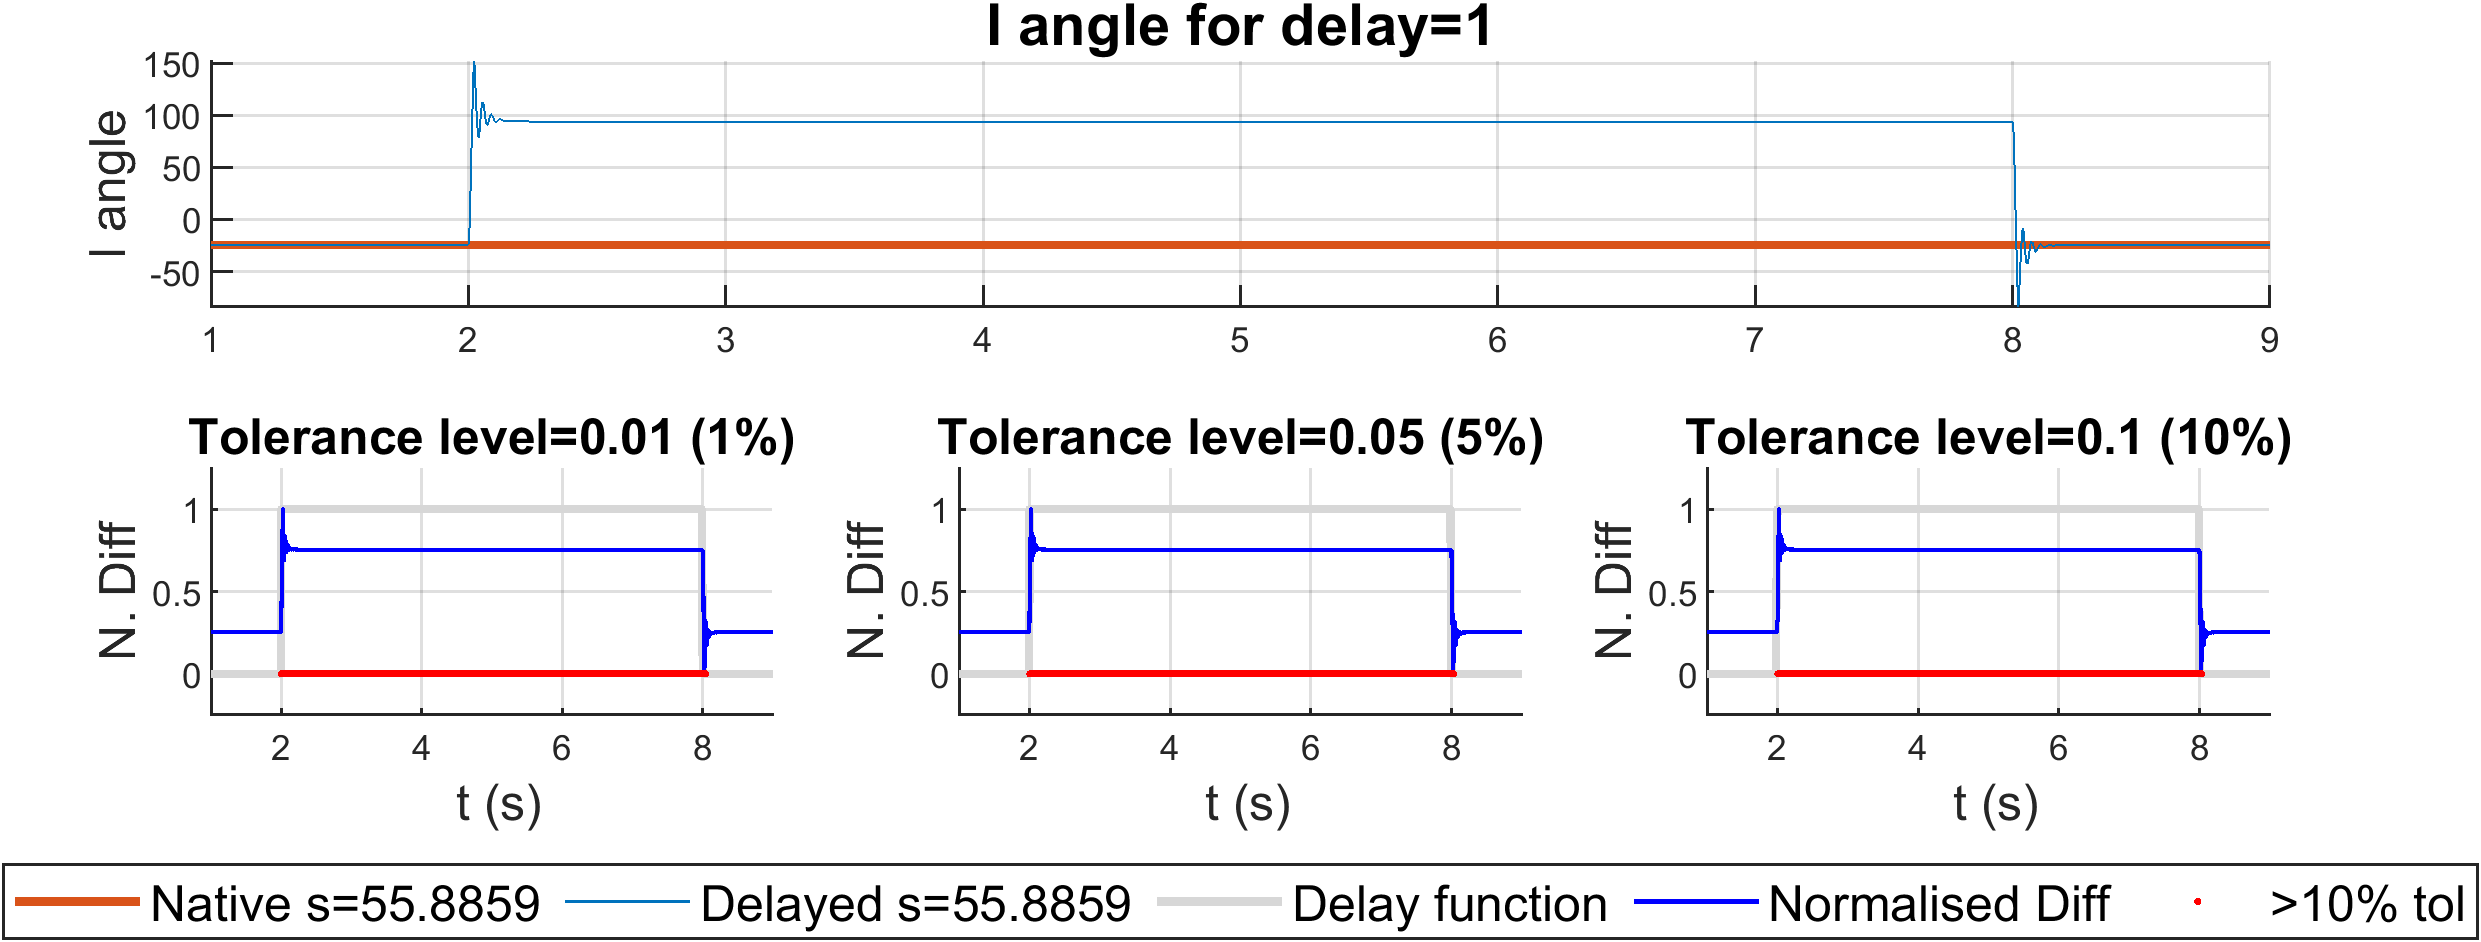
\includegraphics[width=0.95\textwidth]{PMUsim-figures/DelayOf_1/Instant_iAngle.png}    
      \label{fig:PMUsim_One_Angle}
\end{floatingfigure}
      \begin{small}
     \tcbox[size=small, standard jigsaw, opacityback=0, boxrule=0pt,halign=justify]{
     Comment on the figure:}{
     \begin{itemize}
         \item 
     \end{itemize} }
     \end{small}

\newpage \subsection{Delay Level of Two}
\textbf{Results for Magnitude Output}
\begin{floatingfigure}[p]{\textwidth}
    \caption{Instant Delay Magnitude Output for the Delay Level of Two}
    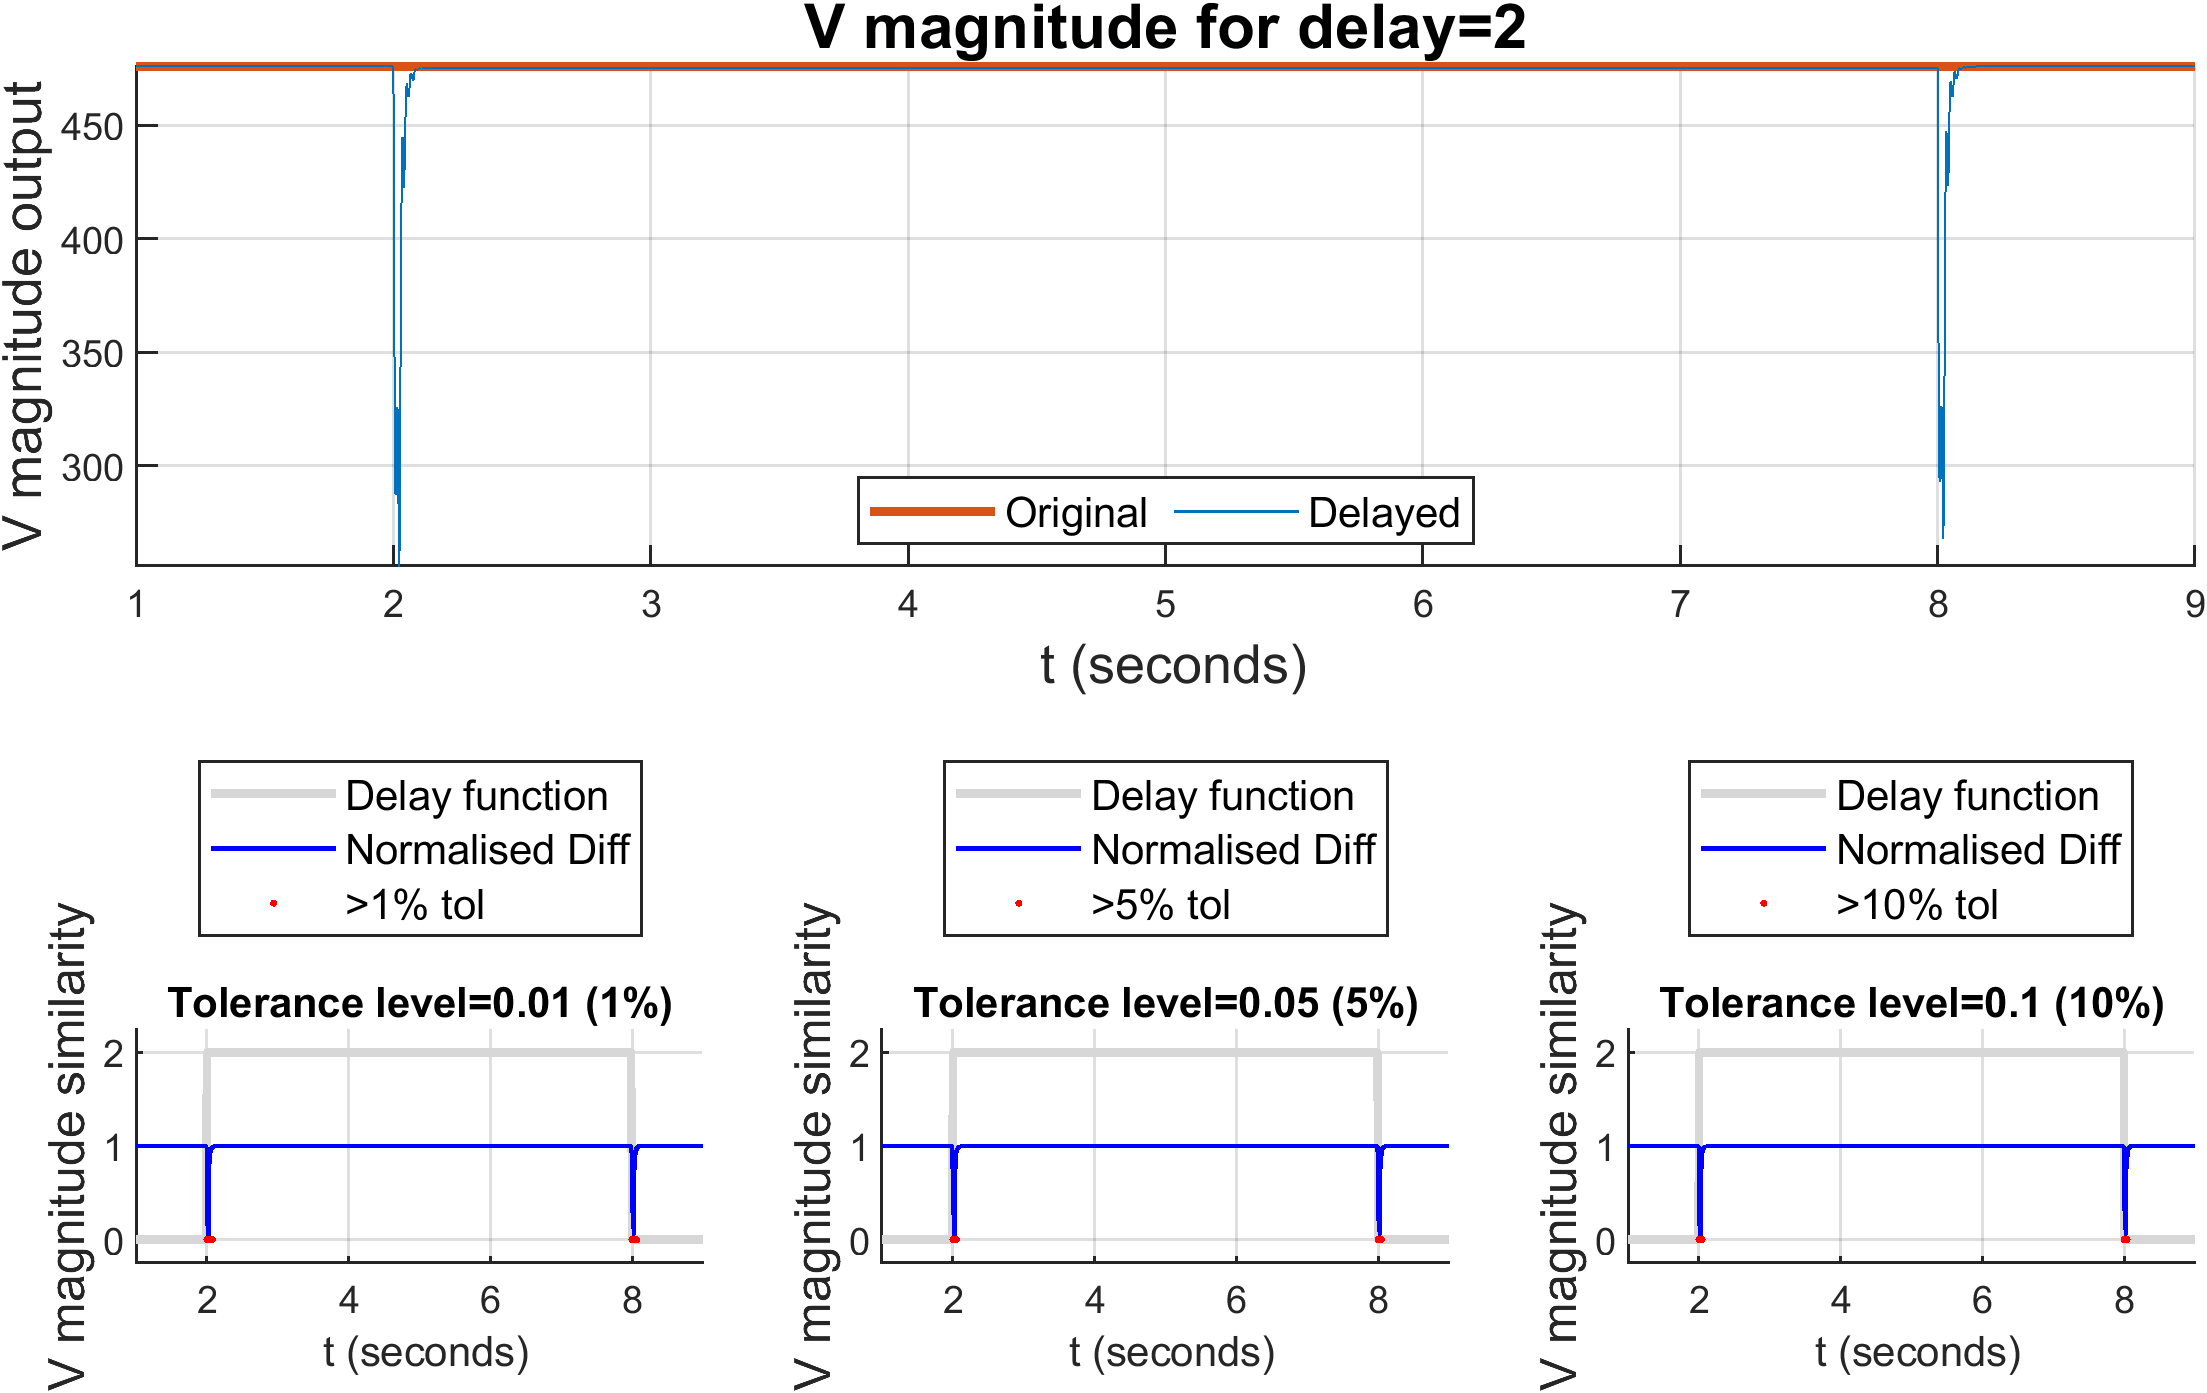
\includegraphics[width=0.95\textwidth]{PMUsim-figures/DelayOf_2/Instant_vMagnitude.png}    
      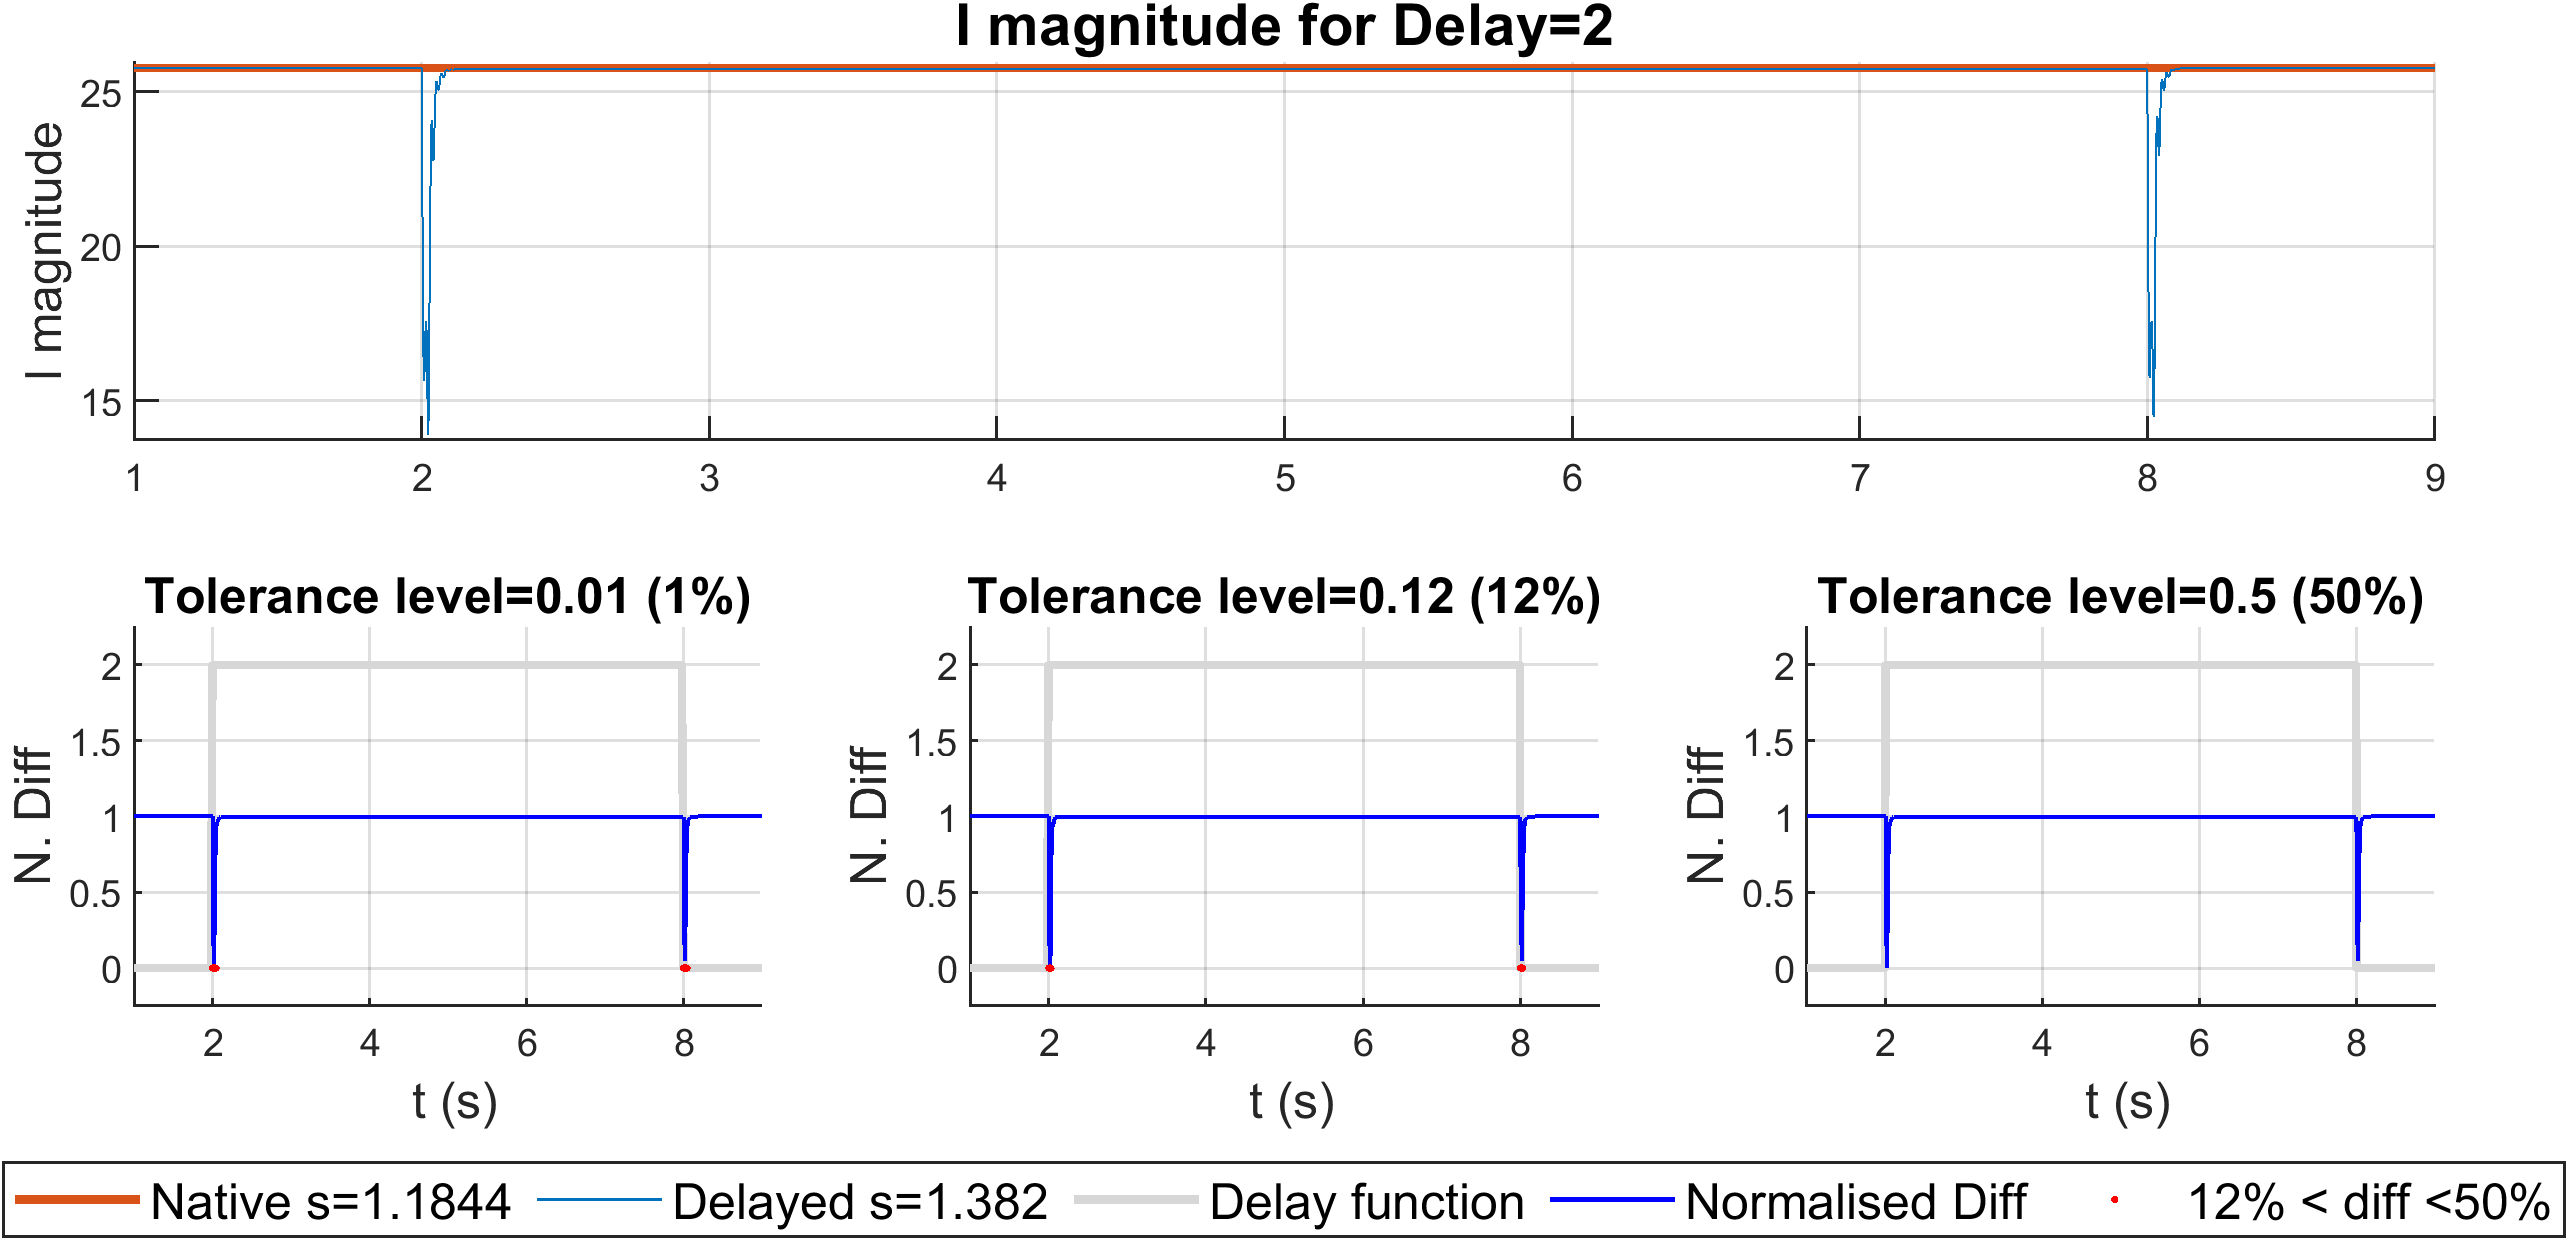
\includegraphics[width=0.95\textwidth]{PMUsim-figures/DelayOf_2/Instant_iMagnitude.png}
    \label{fig:PMUsim_Two_Magnitude}
\end{floatingfigure}
    \begin{small}
     \tcbox[size=small, standard jigsaw, opacityback=0, boxrule=0pt,halign=justify]{
           comment on the figure:}{\begin{itemize}          \item       \end{itemize} }
     \end{small}

\newpage \textbf{Results for Frequency Output}
\begin{floatingfigure}[p]{\textwidth}
    \caption{Instant Delay Frequency Output for the Delay Level of Two}
    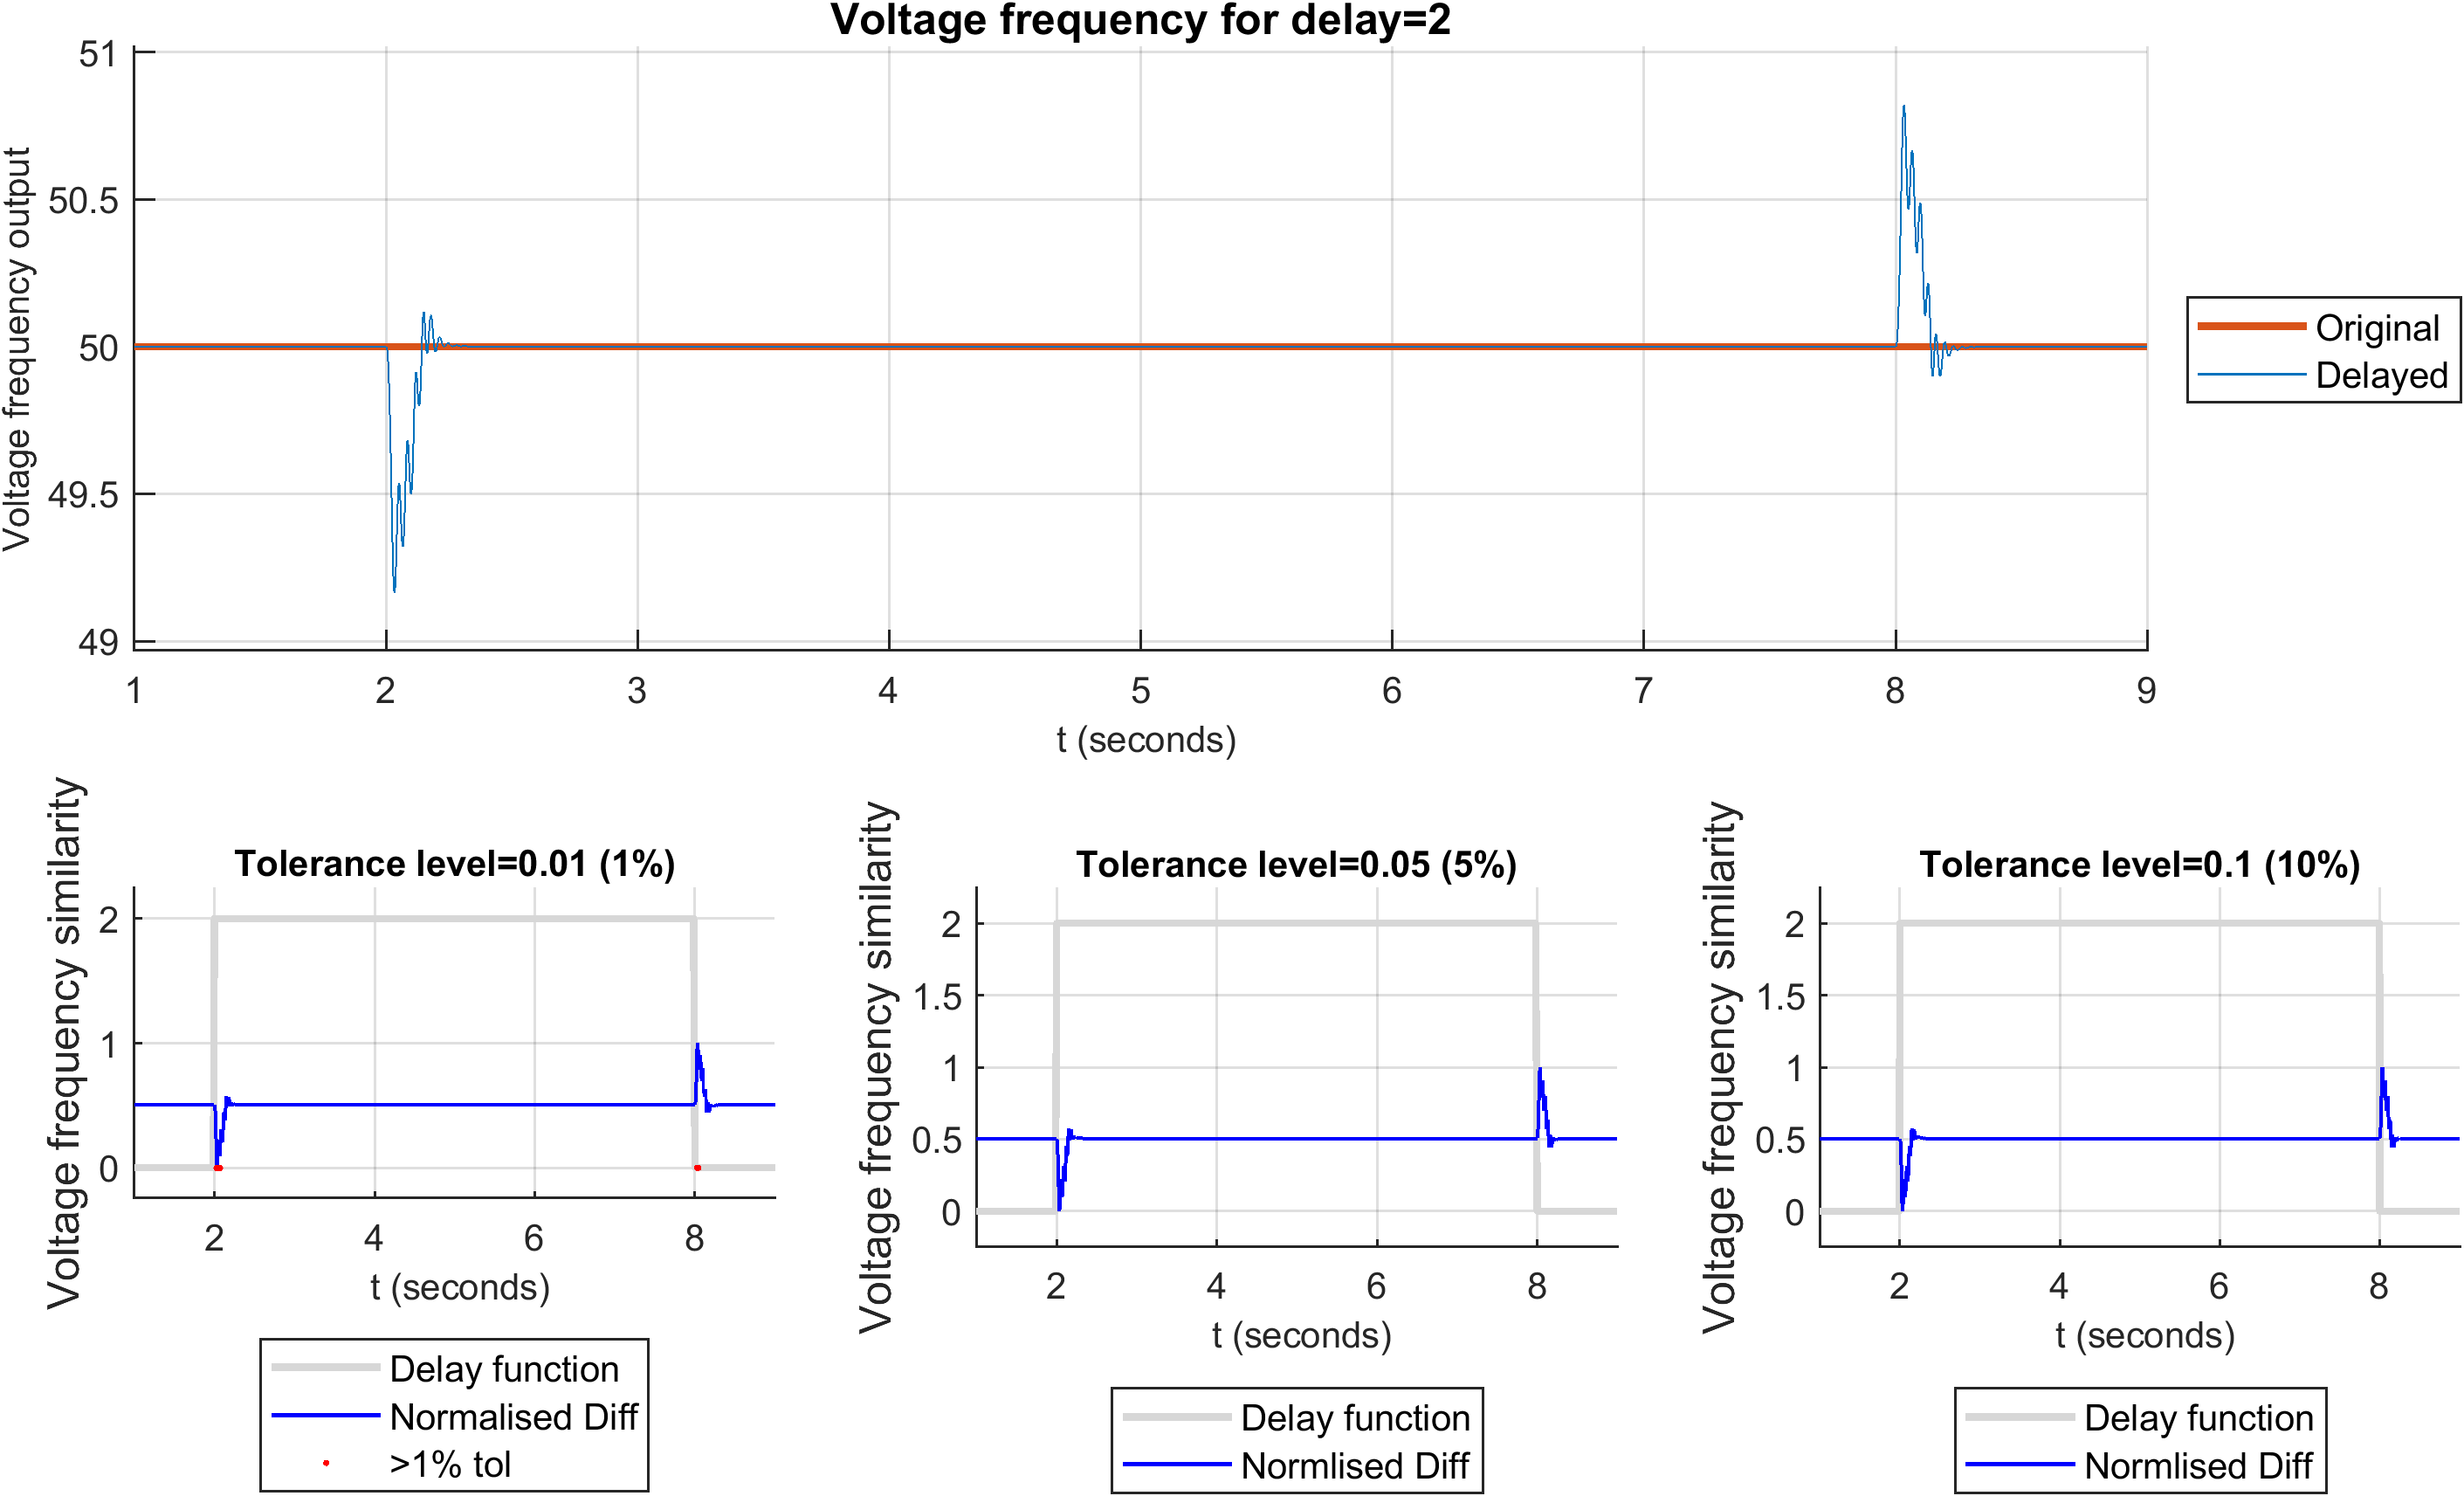
\includegraphics[width=0.95\textwidth]{PMUsim-figures/DelayOf_2/Instant_vFrequency.png}    
    \label{fig:PMUsim_Two_vFrequency}
    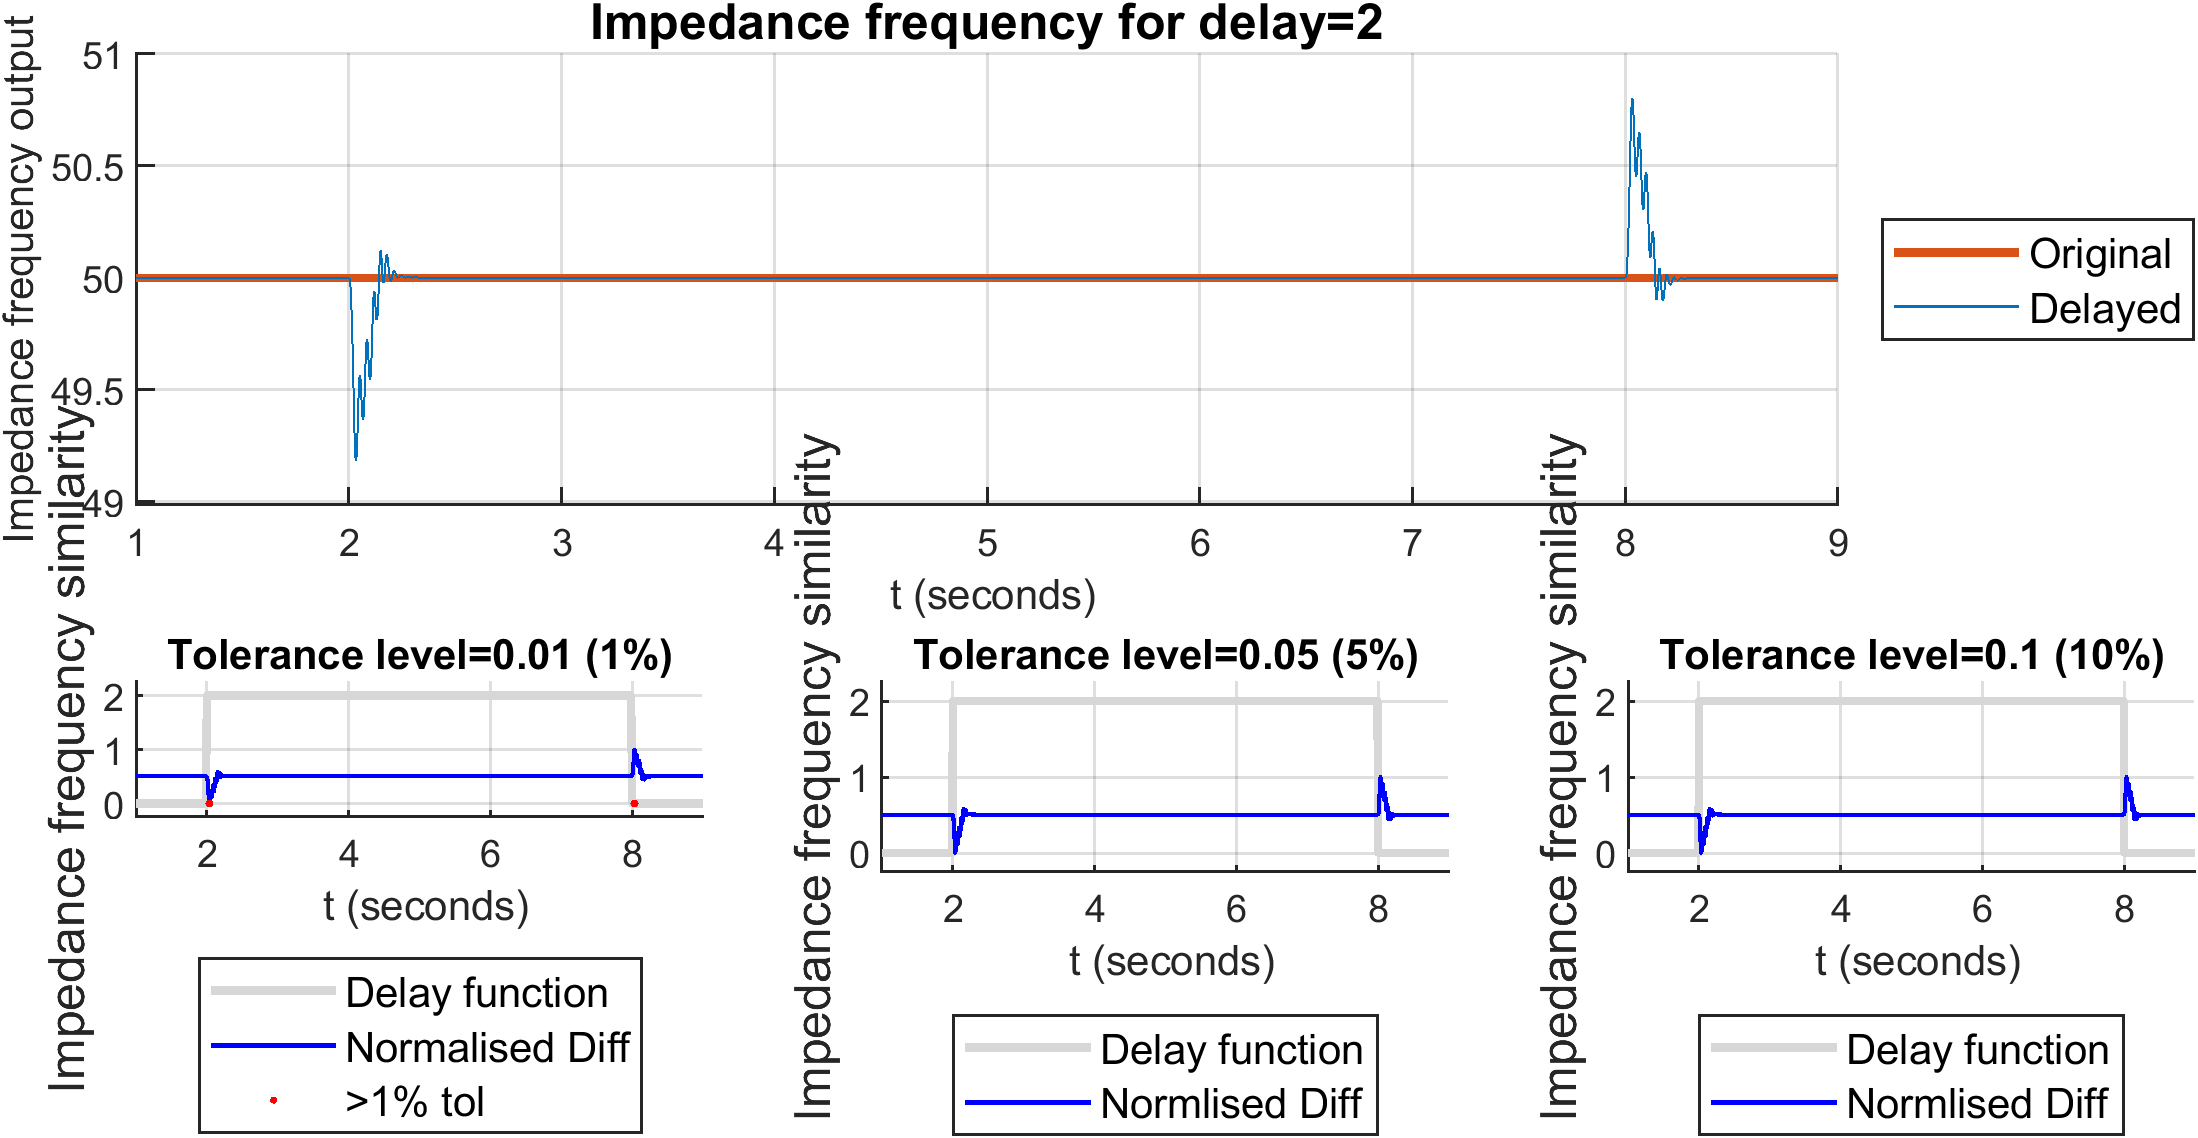
\includegraphics[width=0.95\textwidth]{PMUsim-figures/DelayOf_2/Instant_iFrequency.png}    
    \label{fig:PMUsim_Two_Frequency}
\end{floatingfigure}
        \begin{small}
     \tcbox[size=small, standard jigsaw, opacityback=0, boxrule=0pt,halign=justify]{
     Comment on the figure:}{
     \begin{itemize}
         \item 
     \end{itemize} }
     \end{small}


\newpage \textbf{Results for Angle Output}


\begin{floatingfigure}[p]{\textwidth}
    \caption{Instant Delay Angle Output for the Delay Level of Two}
    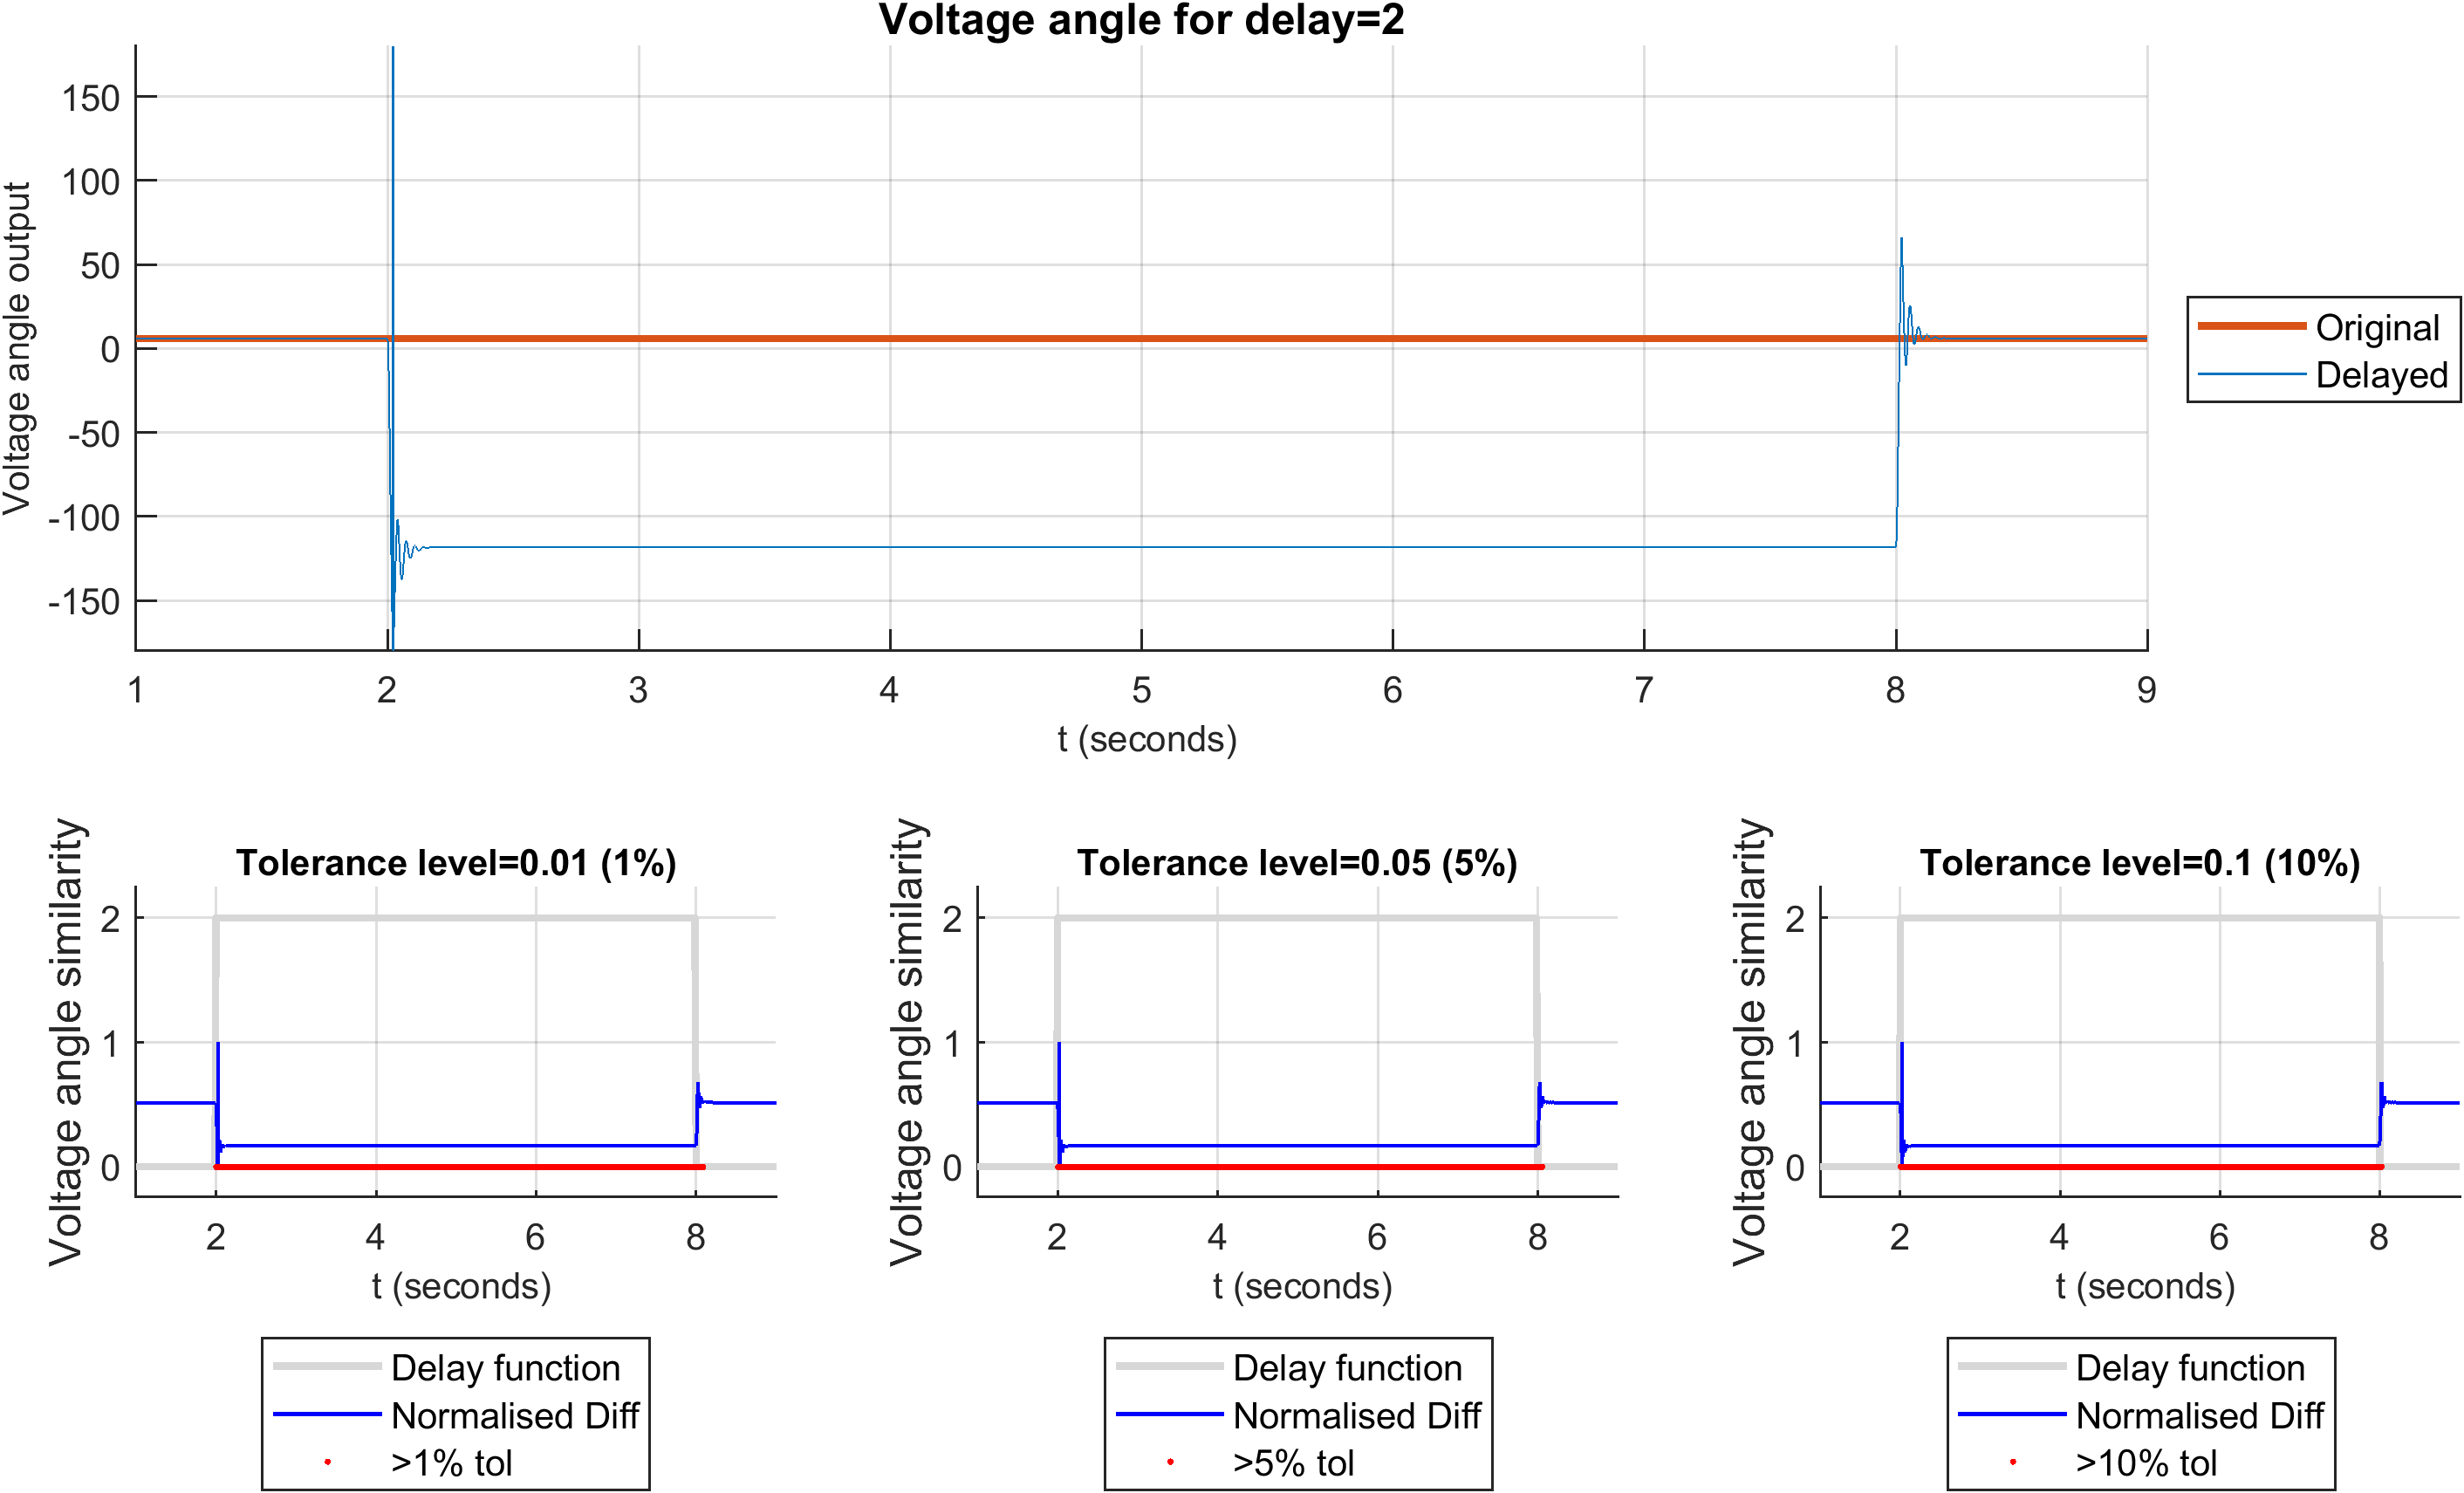
\includegraphics[width=0.95\textwidth]{PMUsim-figures/DelayOf_2/Instant_vAngle.png}    
    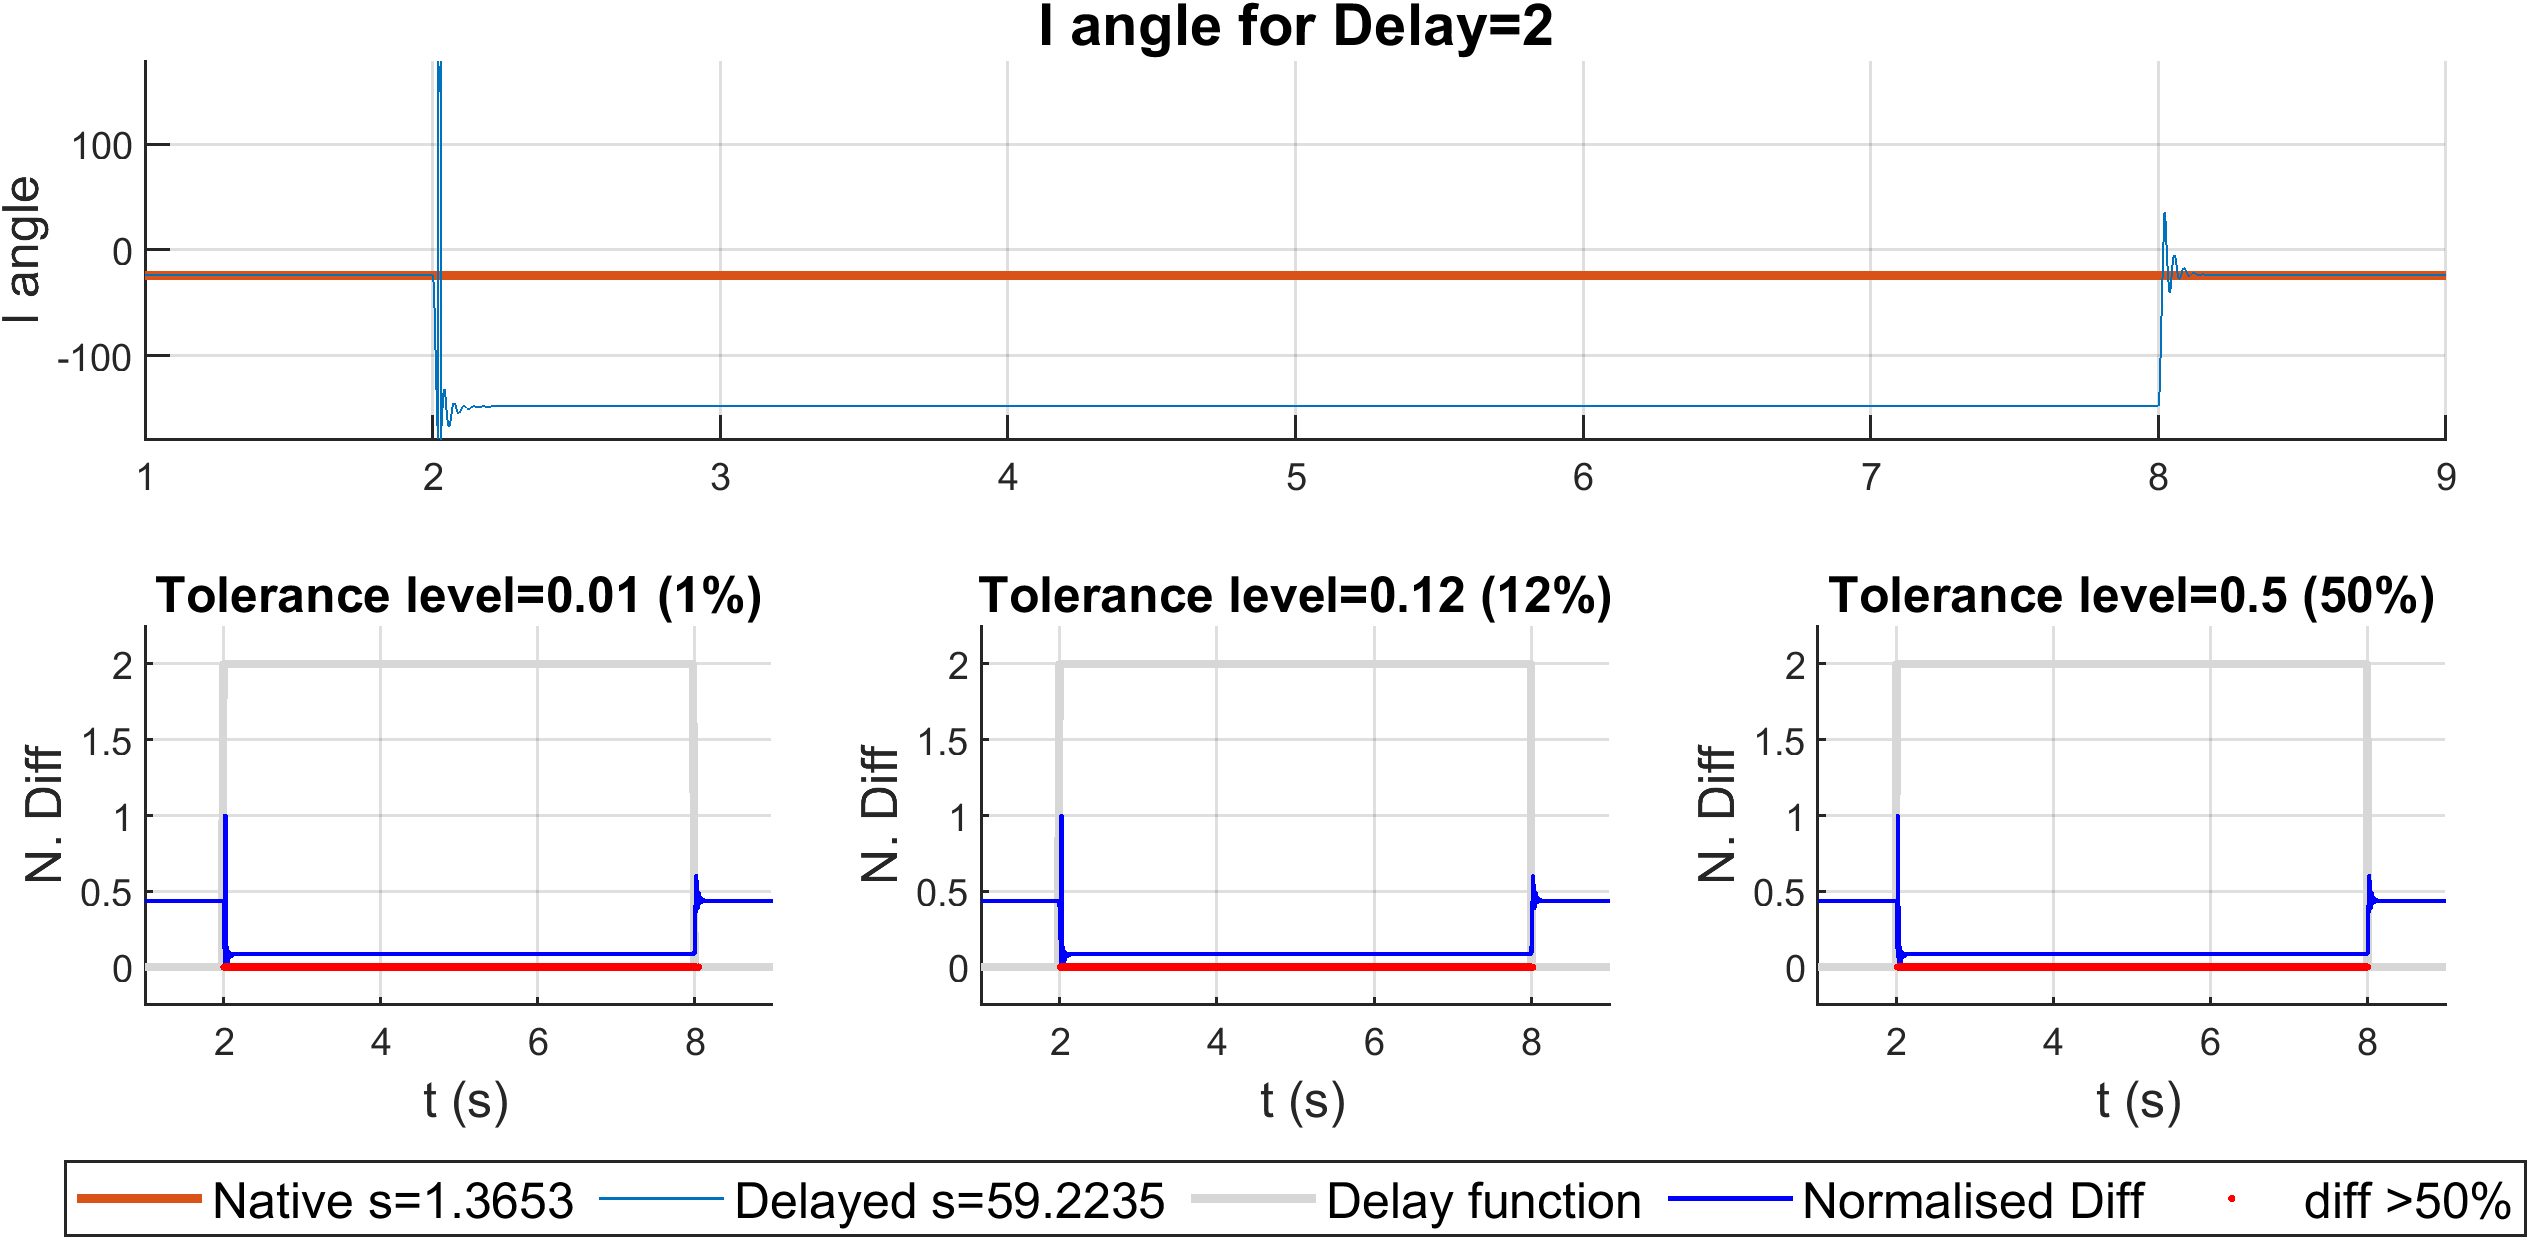
\includegraphics[width=0.95\textwidth]{PMUsim-figures/DelayOf_2/Instant_iAngle.png}    
    \label{fig:PMUsim_Two_Angle}
\end{floatingfigure}

        \begin{small}
     \tcbox[size=small, standard jigsaw, opacityback=0, boxrule=0pt,halign=justify]{
     Comment on the figure:}{
     \begin{itemize}
         \item 
     \end{itemize} }
     \end{small}

\newpage \subsection{Delay Level of Three}
\textbf{Results for Magnitude Output}

\begin{floatingfigure}[p]{\textwidth}
    \caption{Instant Delay Magnitude Output for the Delay Level of Three}
    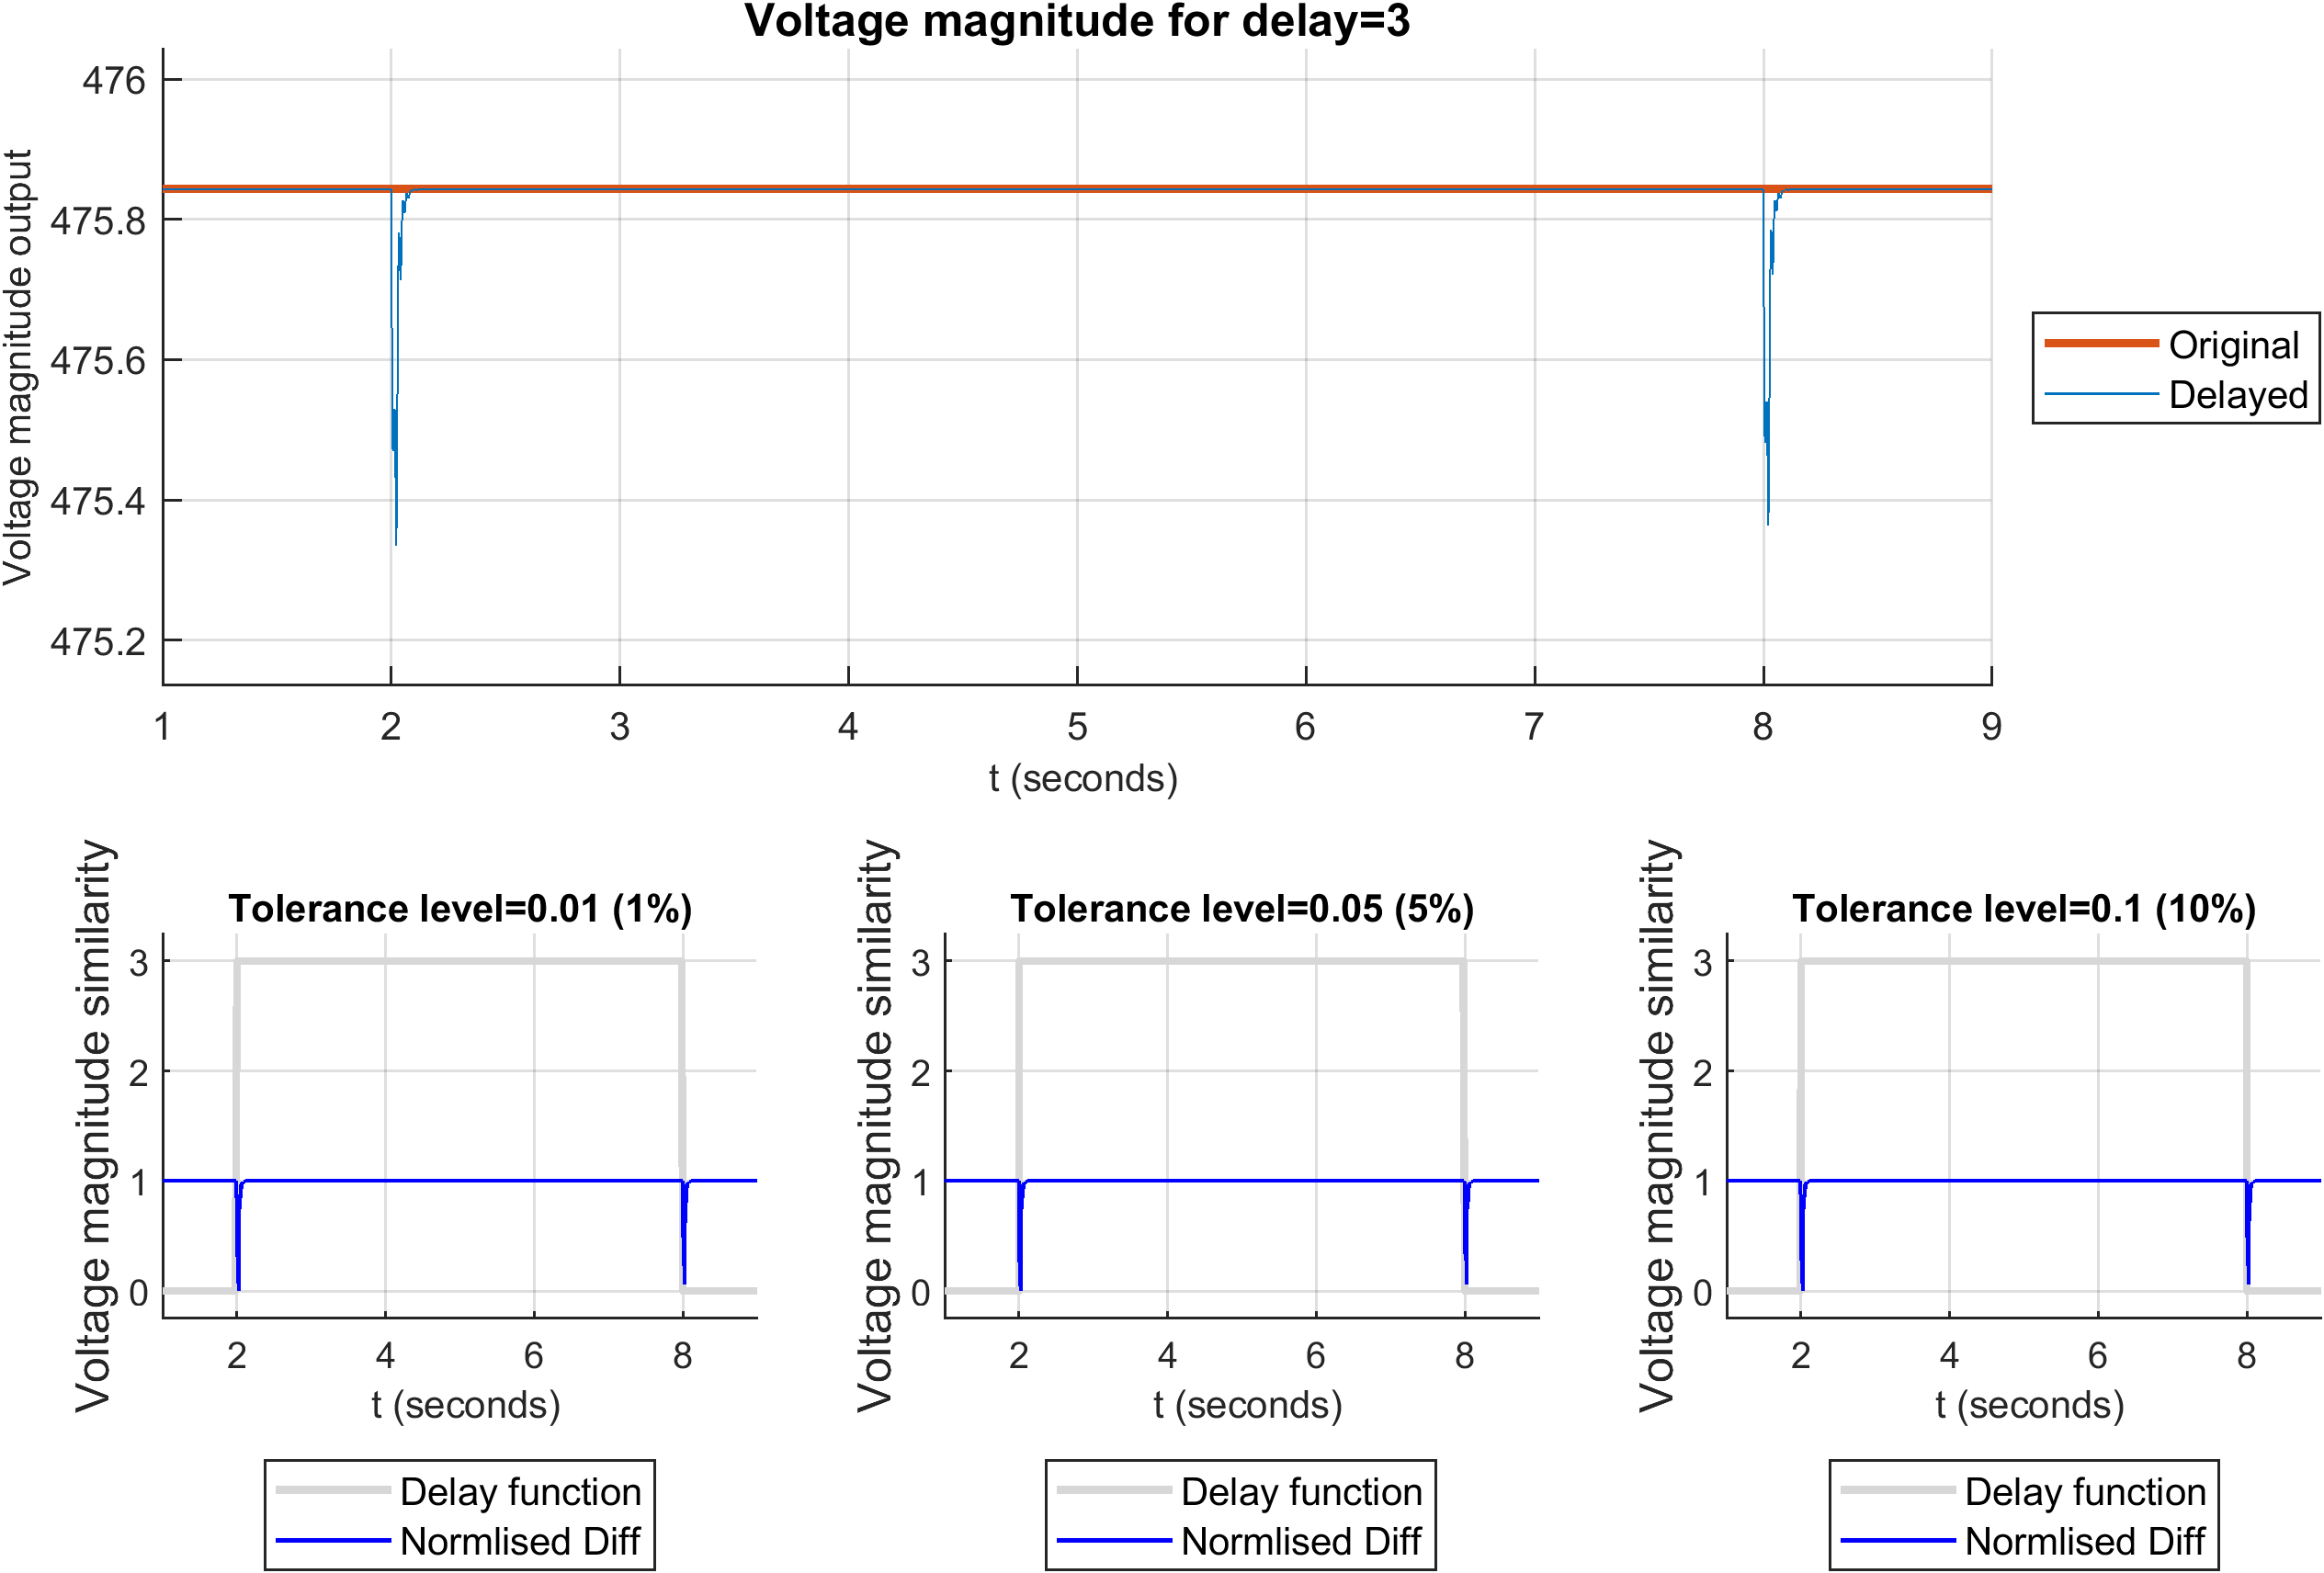
\includegraphics[width=0.95\textwidth]{PMUsim-figures/DelayOf_3/Instant_vMagnitude.png}    
      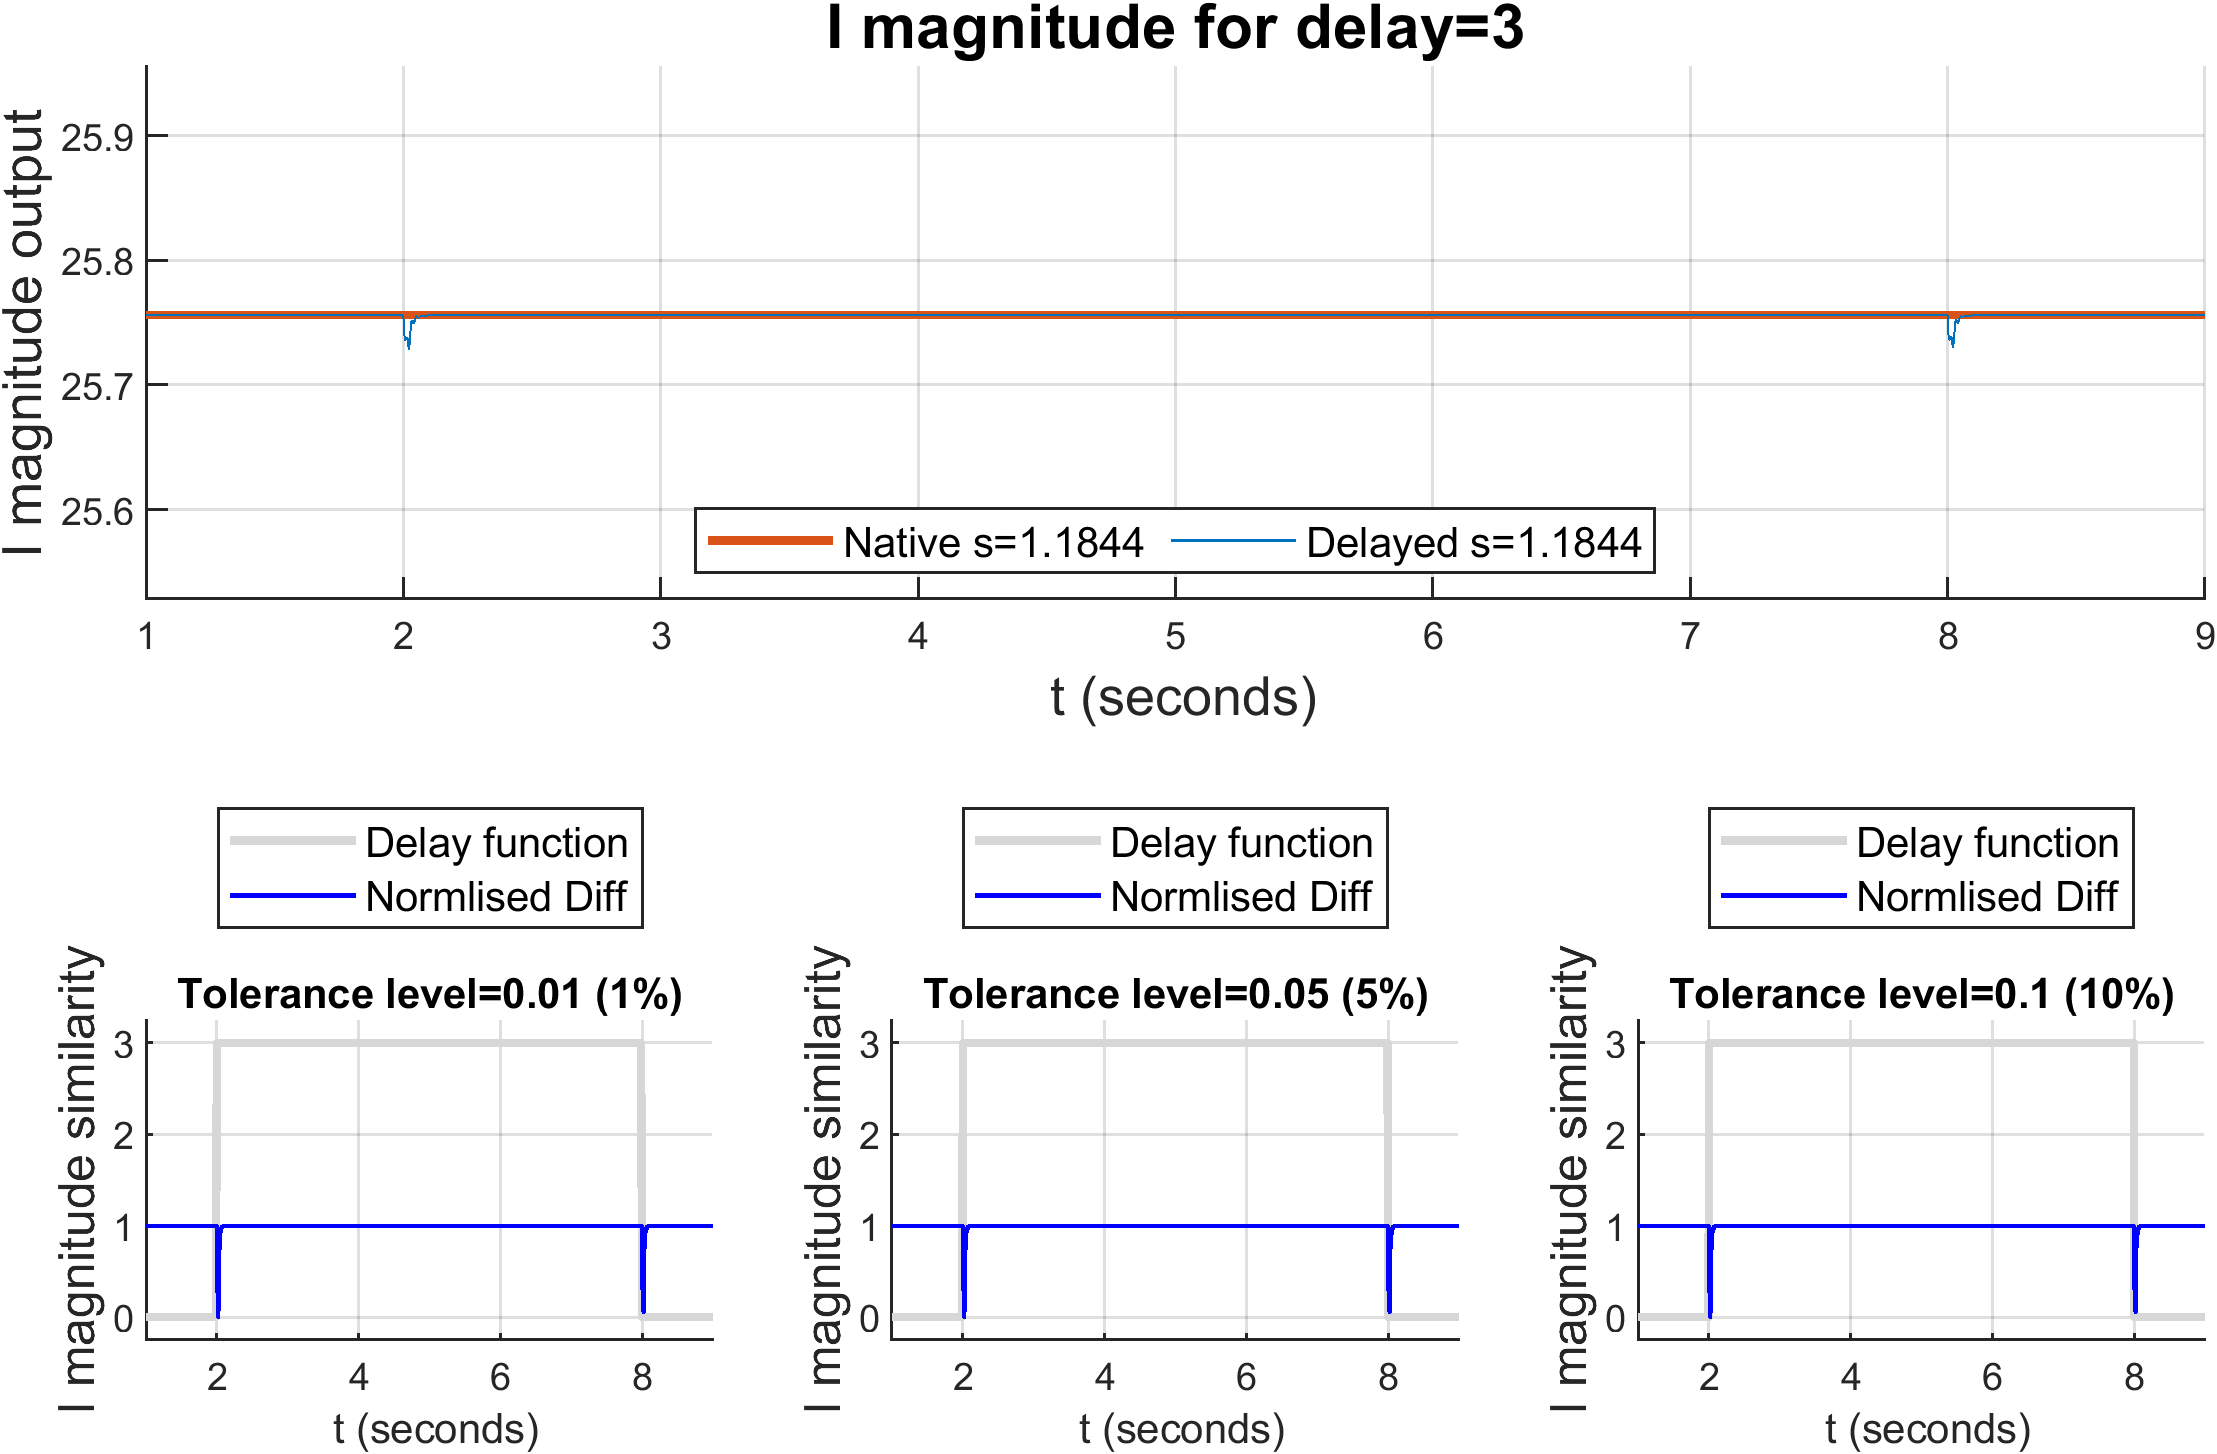
\includegraphics[width=0.95\textwidth]{PMUsim-figures/DelayOf_3/Instant_iMagnitude.png}
    \label{fig:PMUsim_Three_Magnitude}
\end{floatingfigure}
    \begin{small}
     \tcbox[size=small, standard jigsaw, opacityback=0, boxrule=0pt,halign=justify]{
           comment on the figure:}{\begin{itemize}          \item       \end{itemize} }
     \end{small}

\newpage \textbf{Results for Frequency Output}


\begin{floatingfigure}[p]{\textwidth}
    \caption{Instant Delay Frequency Output for the Delay Level of Three}
    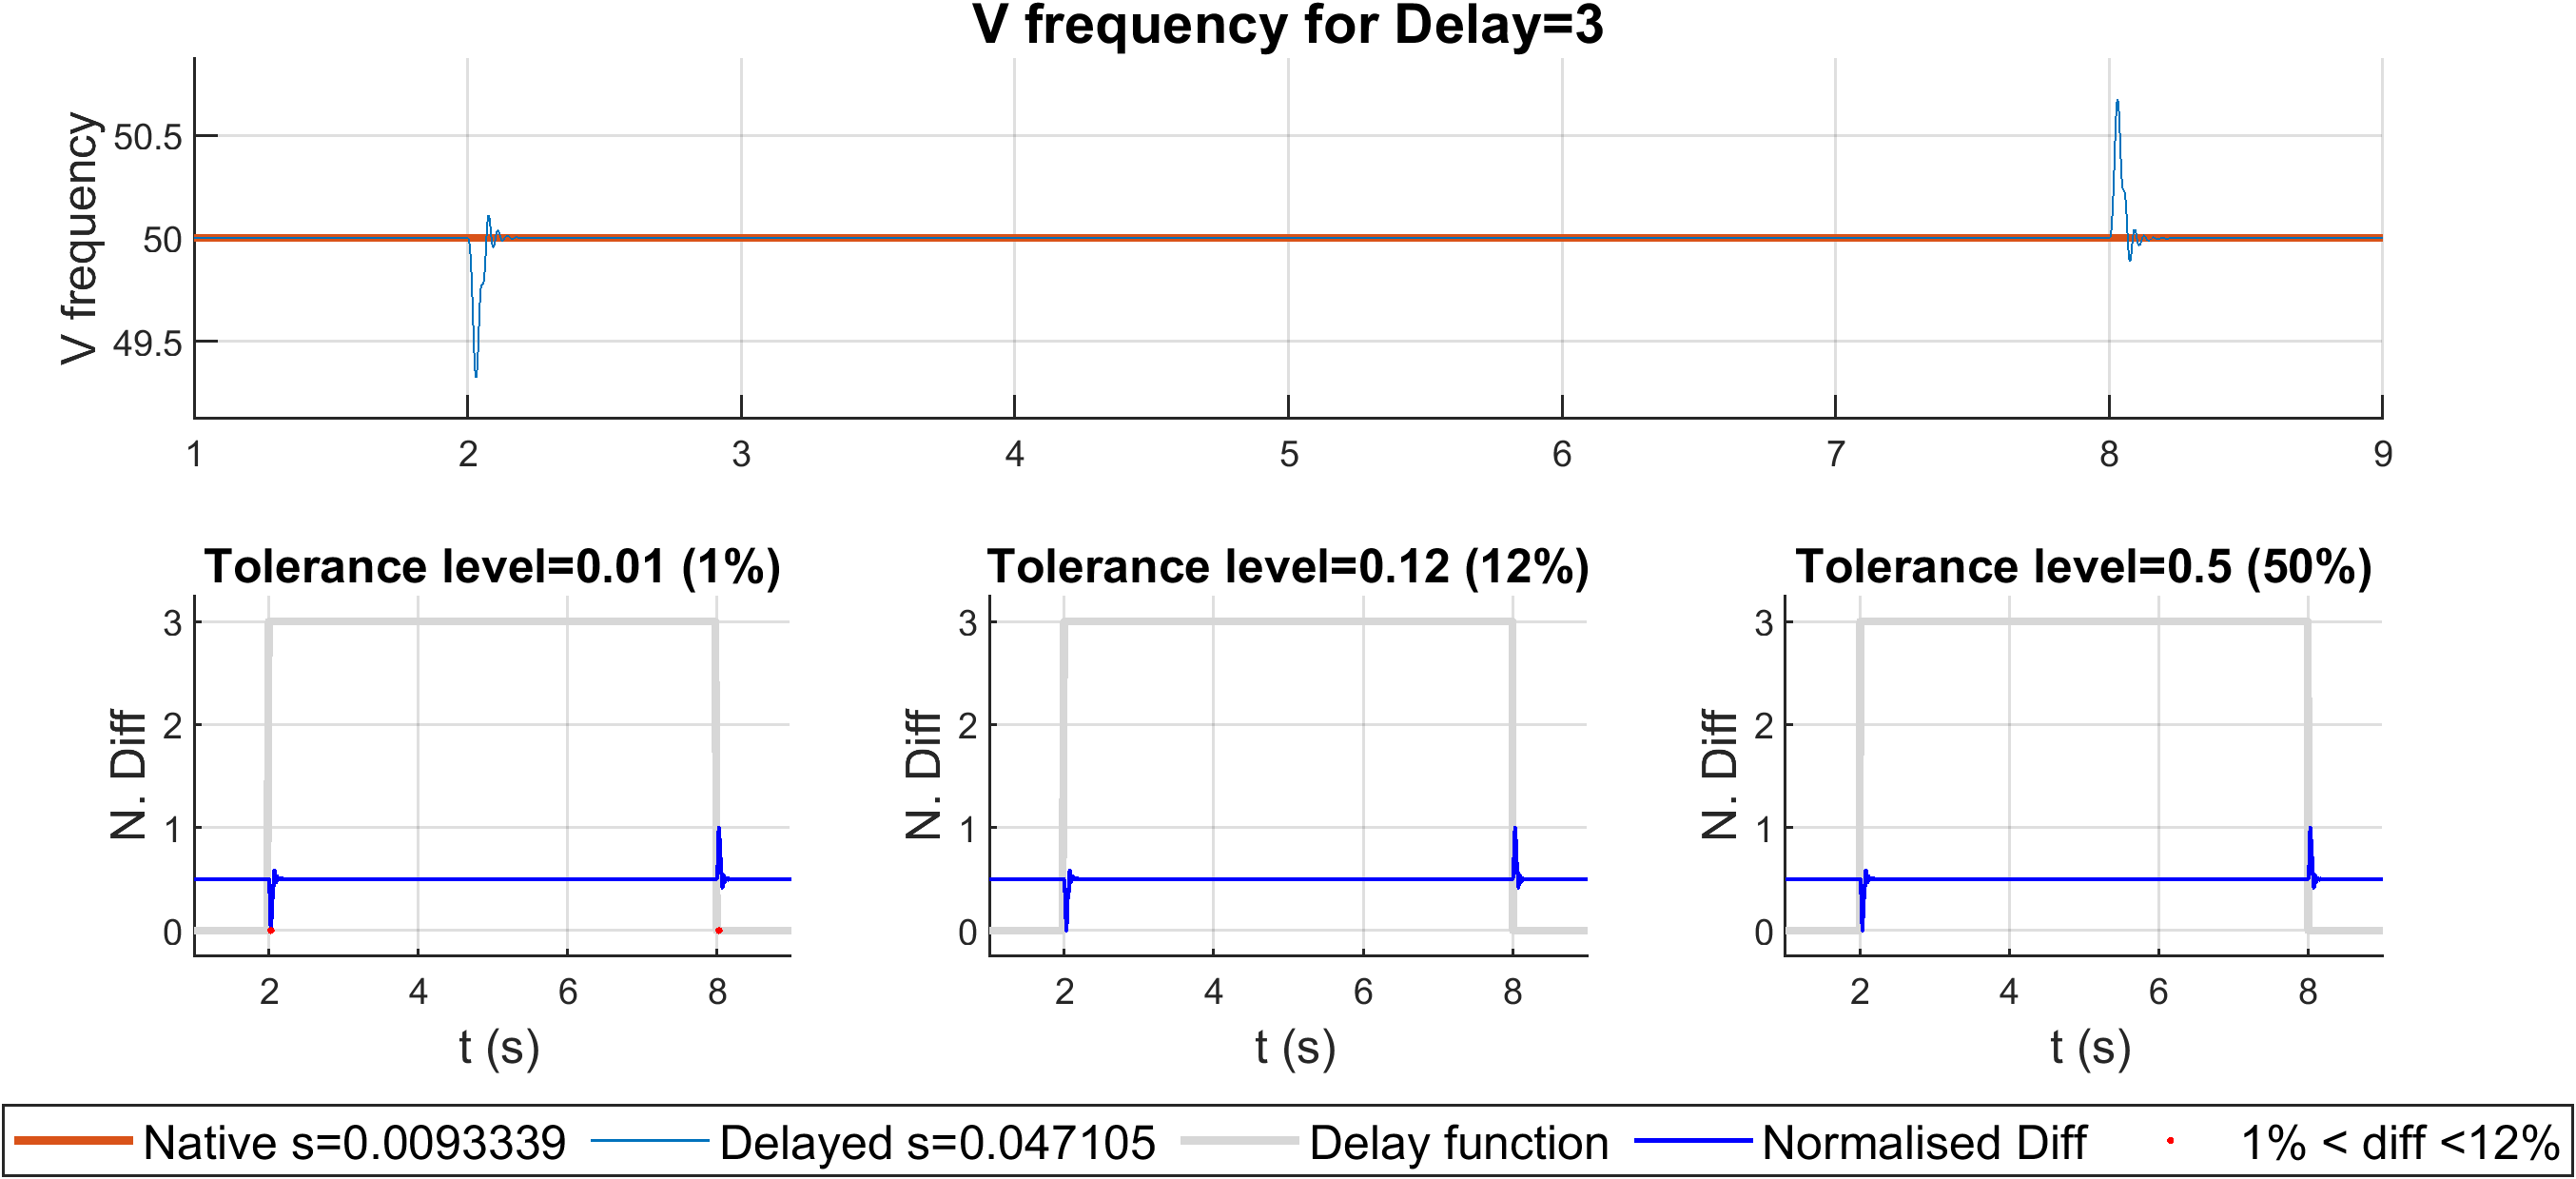
\includegraphics[width=0.95\textwidth]{PMUsim-figures/DelayOf_3/Instant_vFrequency.png}    
    \label{fig:PMUsim_Three_vFrequency}
    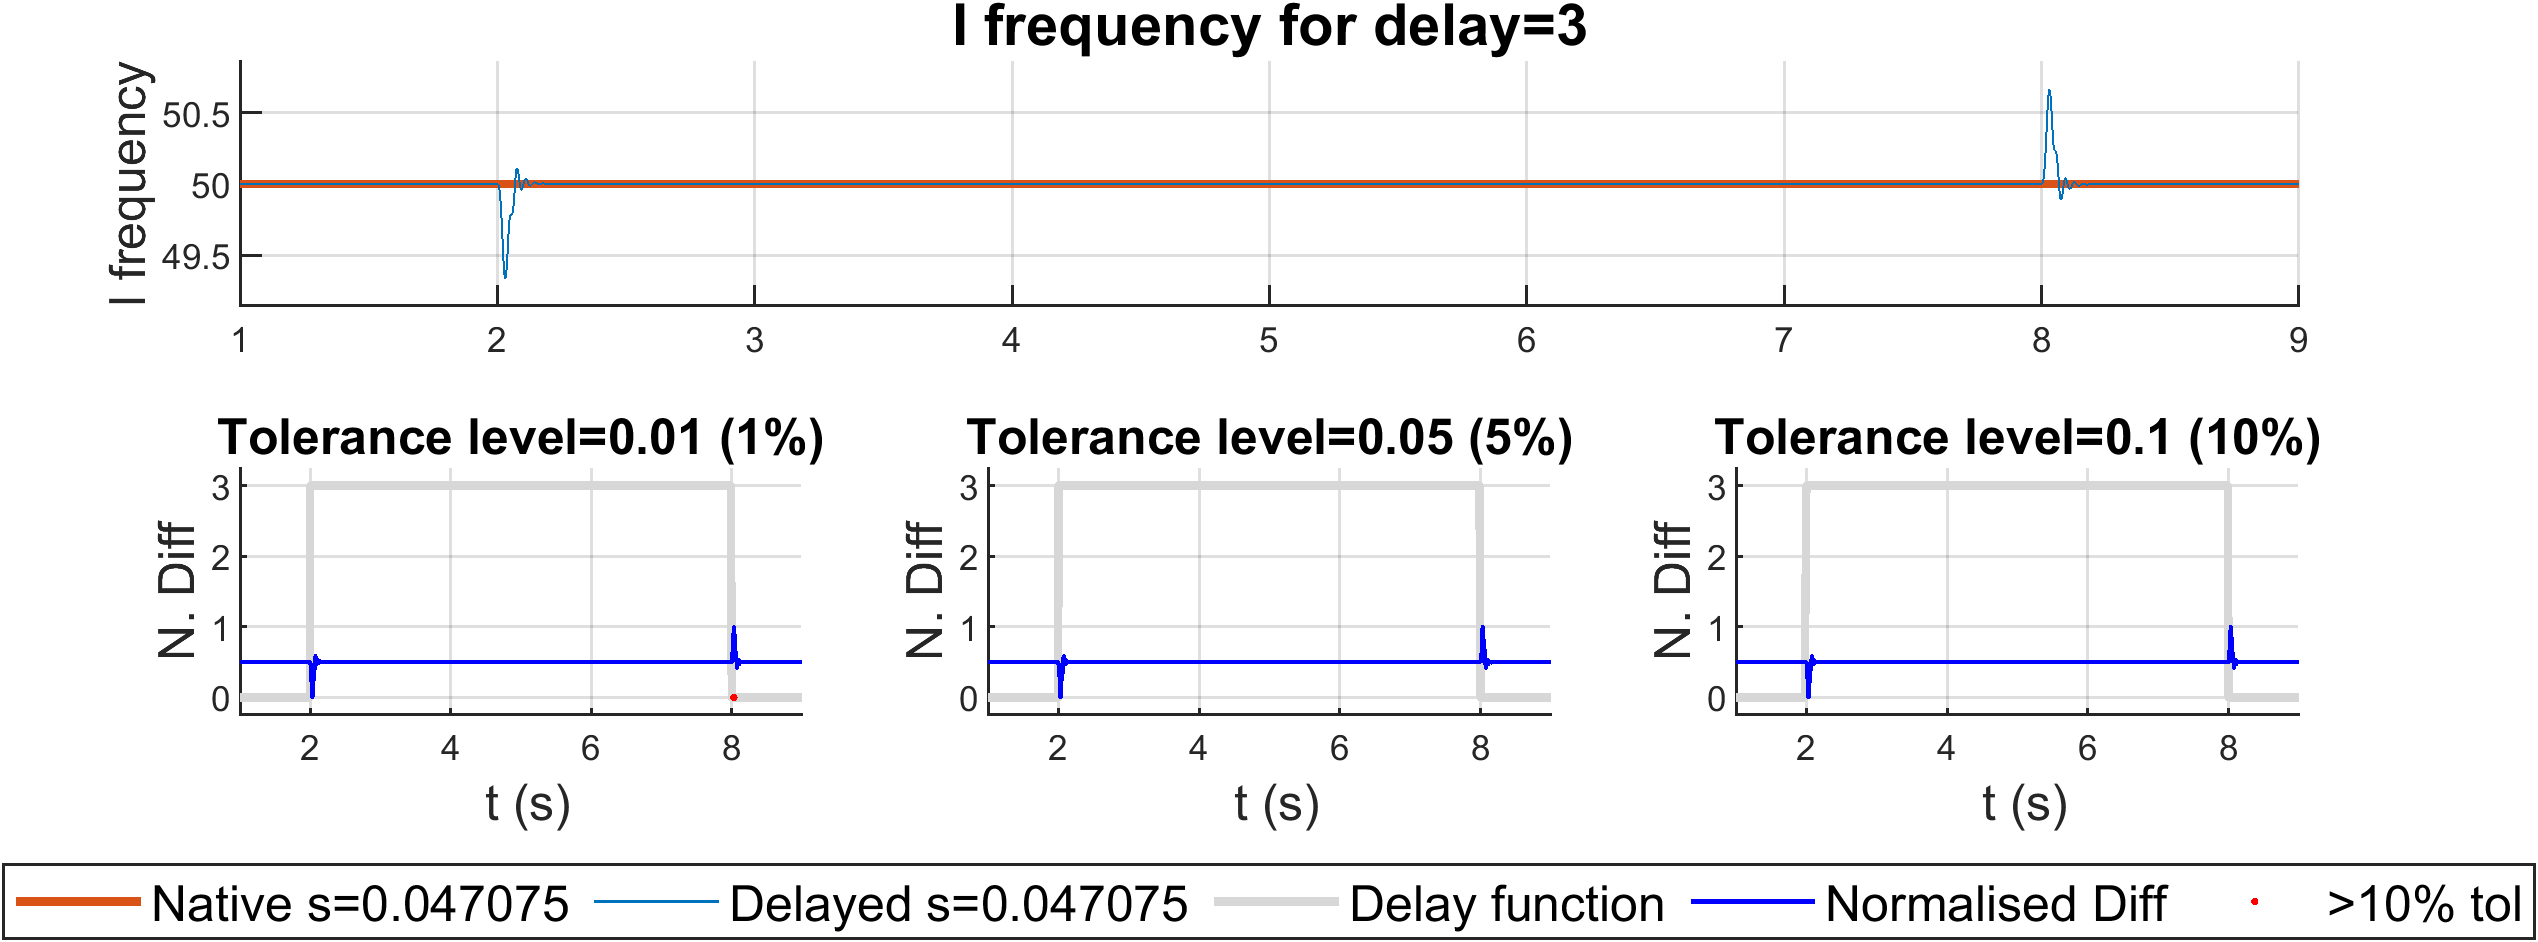
\includegraphics[width=0.95\textwidth]{PMUsim-figures/DelayOf_3/Instant_iFrequency.png}    
    \label{fig:PMUsim_Three_Frequency}
\end{floatingfigure}
        \begin{small}
     \tcbox[size=small, standard jigsaw, opacityback=0, boxrule=0pt,halign=justify]{
     Comment on the figure:}{
     \begin{itemize}
         \item 
     \end{itemize} }
     \end{small}


\newpage \textbf{Results for Angle Output}


\begin{floatingfigure}[p]{\textwidth}
    \caption{Instant Delay Angle Output for the Delay Level of Three}
    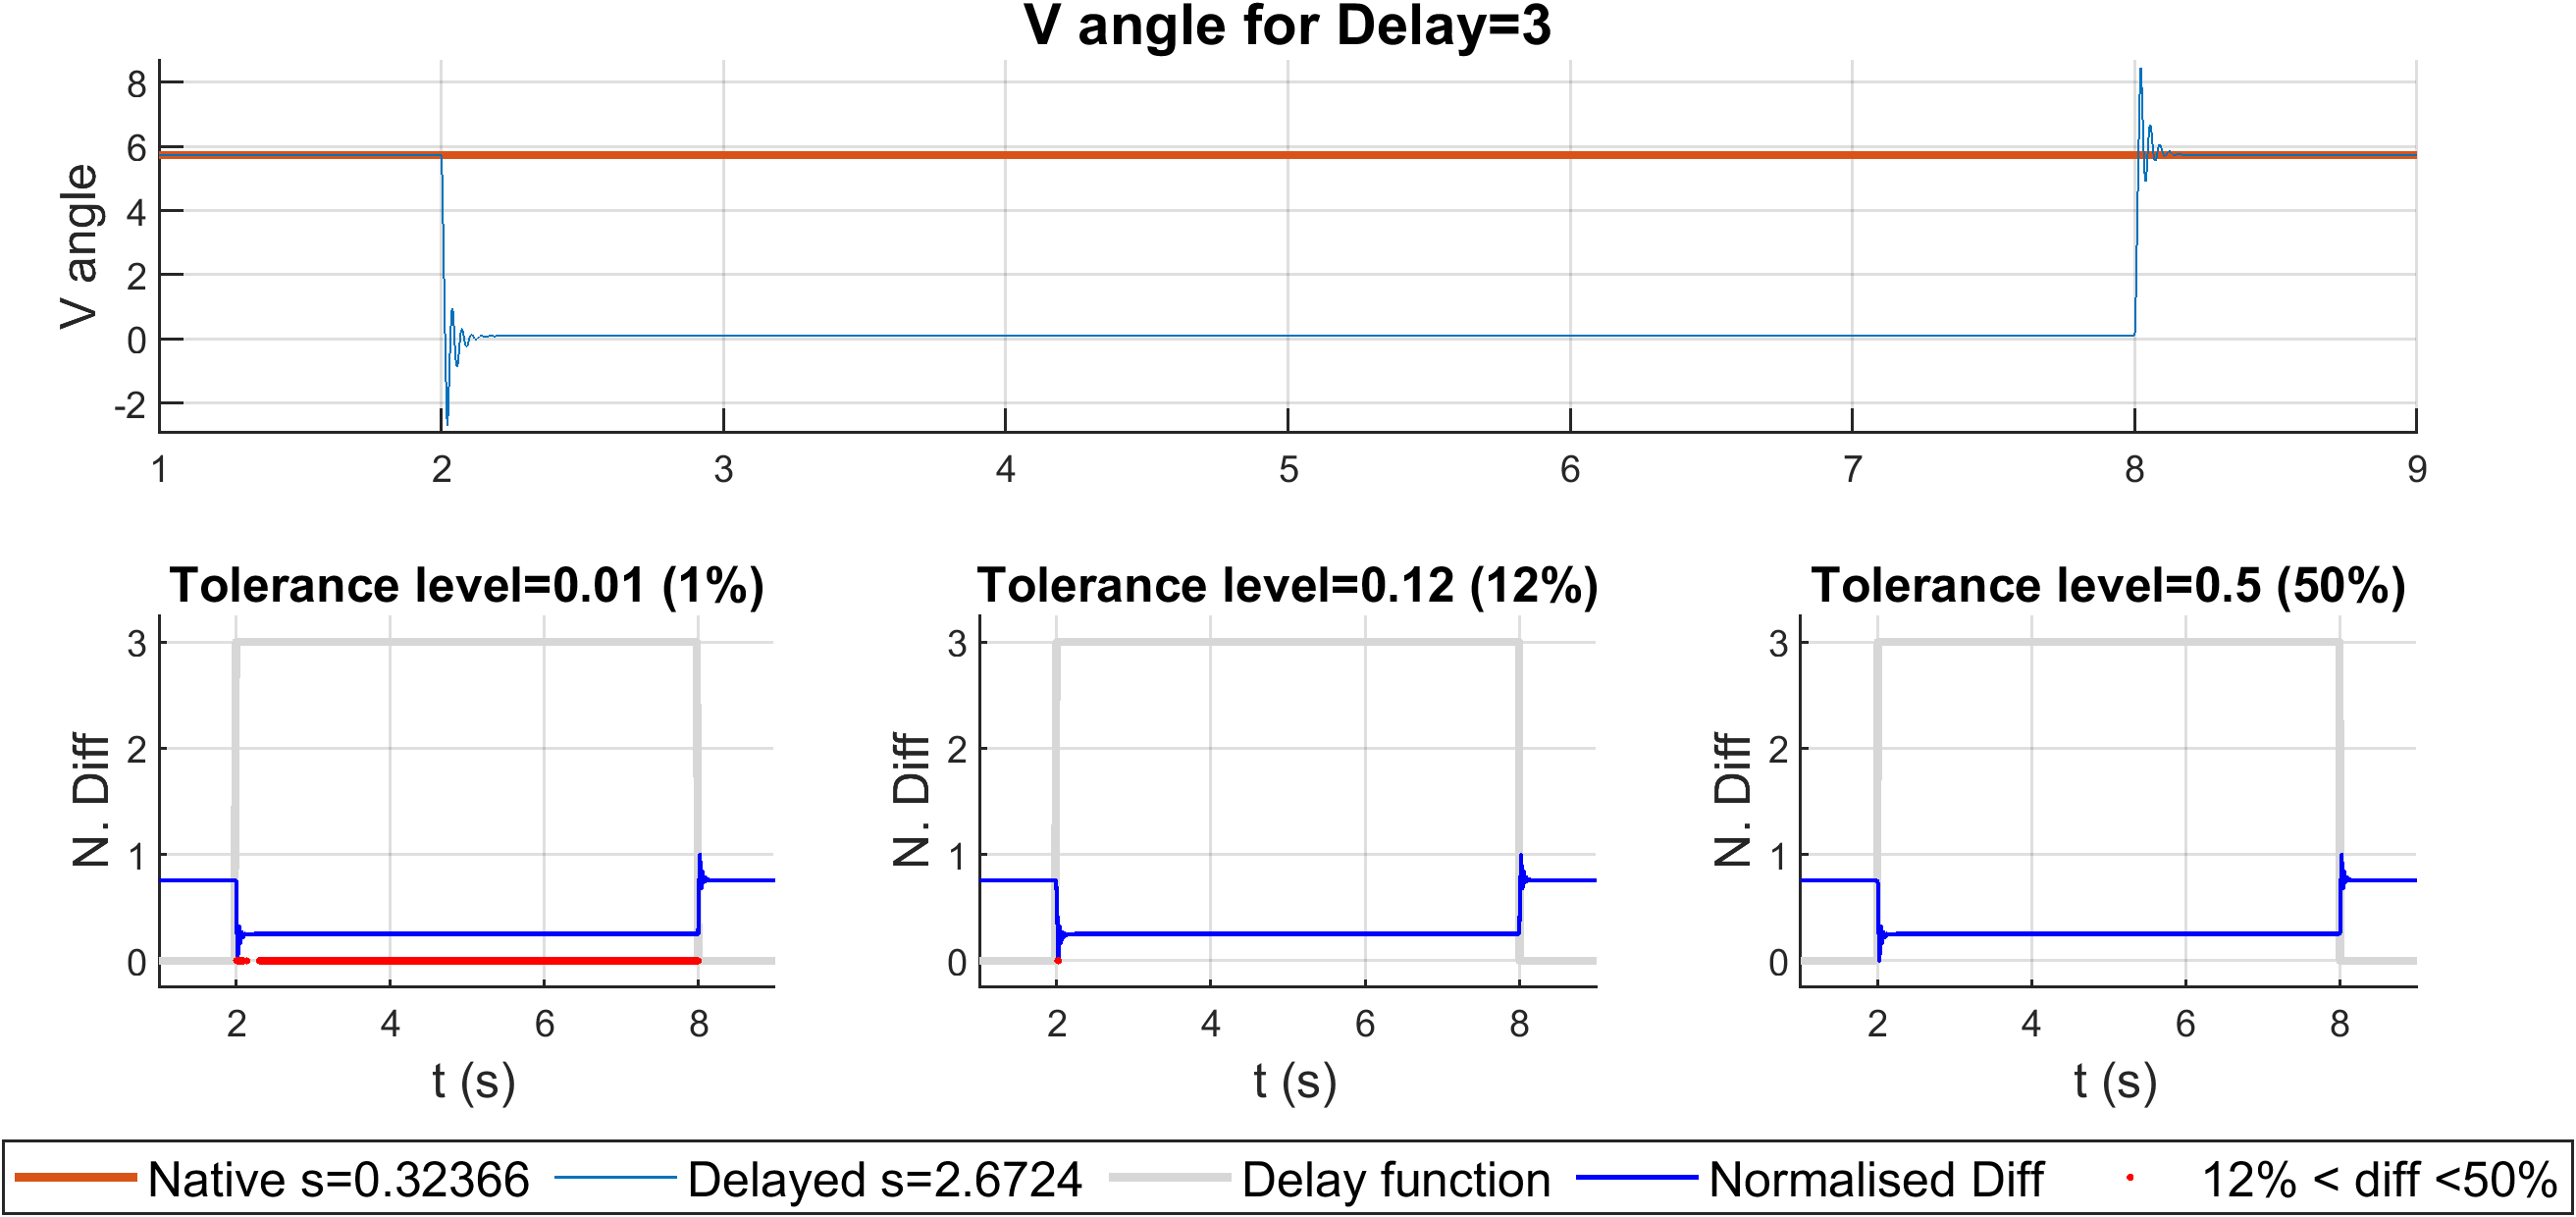
\includegraphics[width=0.95\textwidth]{PMUsim-figures/DelayOf_3/Instant_vAngle.png}    
    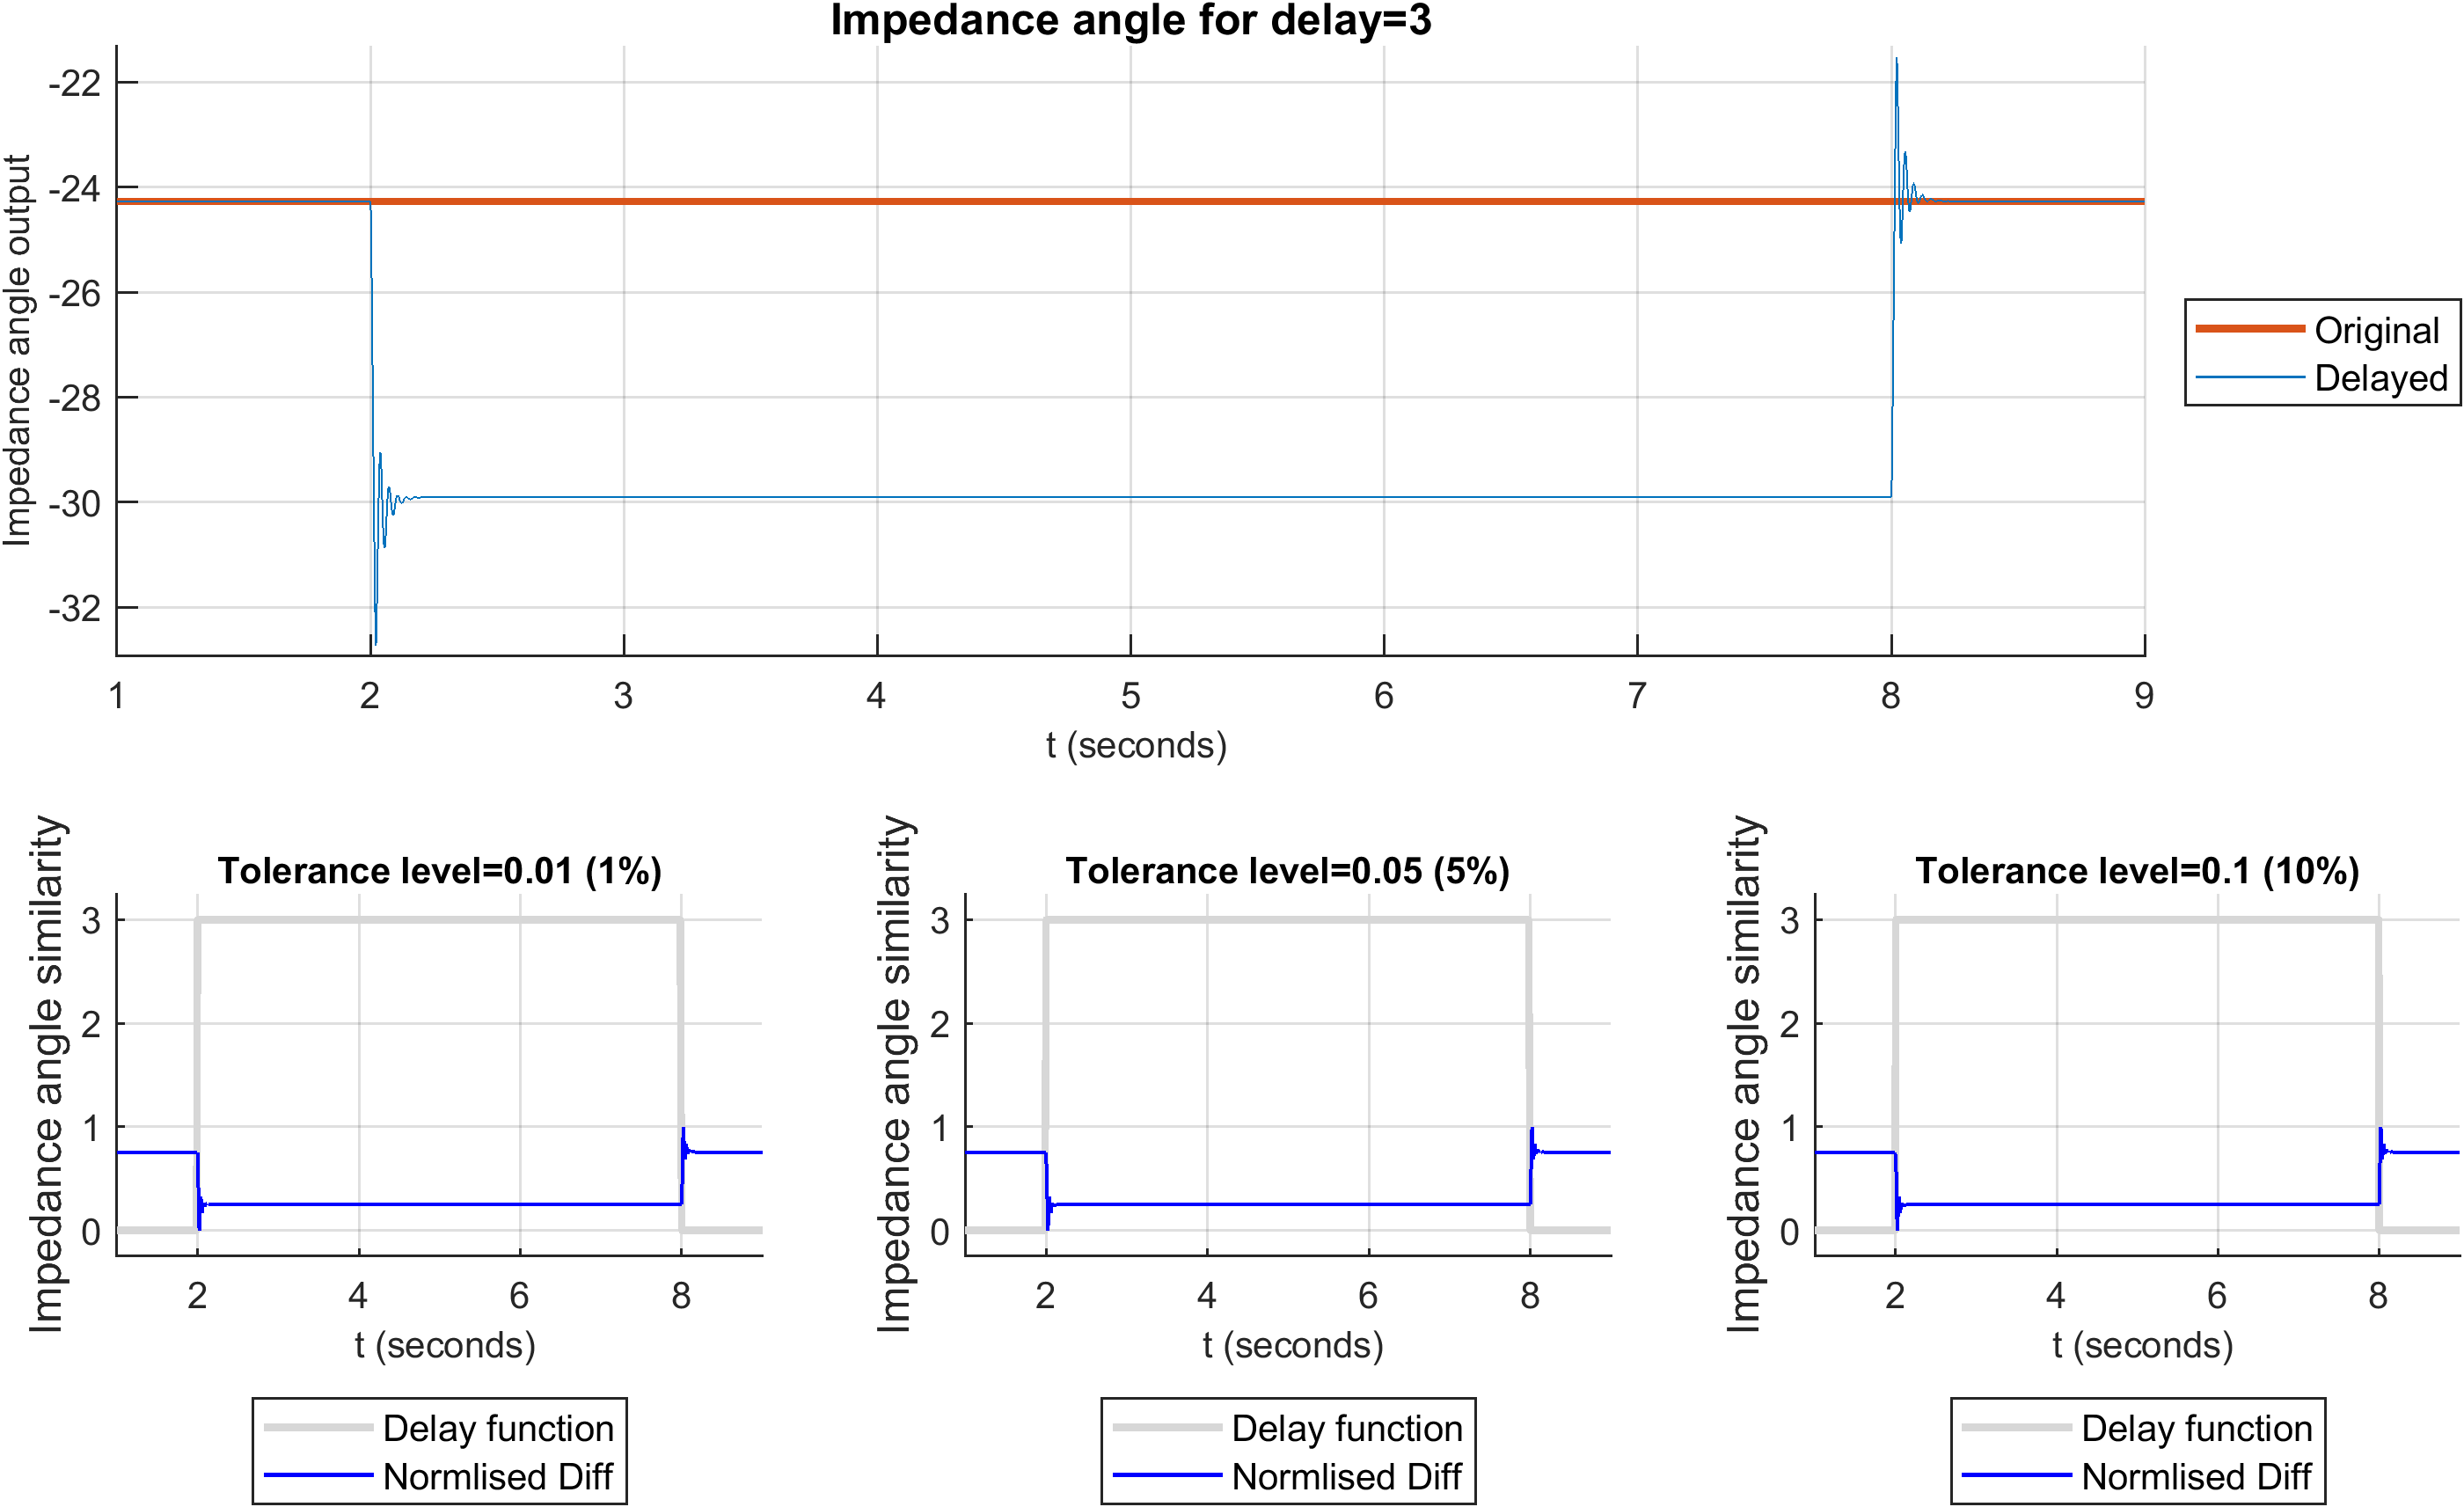
\includegraphics[width=0.95\textwidth]{PMUsim-figures/DelayOf_3/Instant_iAngle.png}    
    \label{fig:PMUsim_Three_Angle}
\end{floatingfigure}
        \begin{small}
     \tcbox[size=small, standard jigsaw, opacityback=0, boxrule=0pt,halign=justify]{
     Comment on the figure:}{
     \begin{itemize}
         \item 
     \end{itemize} }
     \end{small}


\newpage \subsection{Delay Level of Four}
\textbf{Results for Magnitude Output}

\begin{floatingfigure}[p]{\textwidth}
    \caption{Instant Delay Magnitude Output for the Delay Level of Four}
    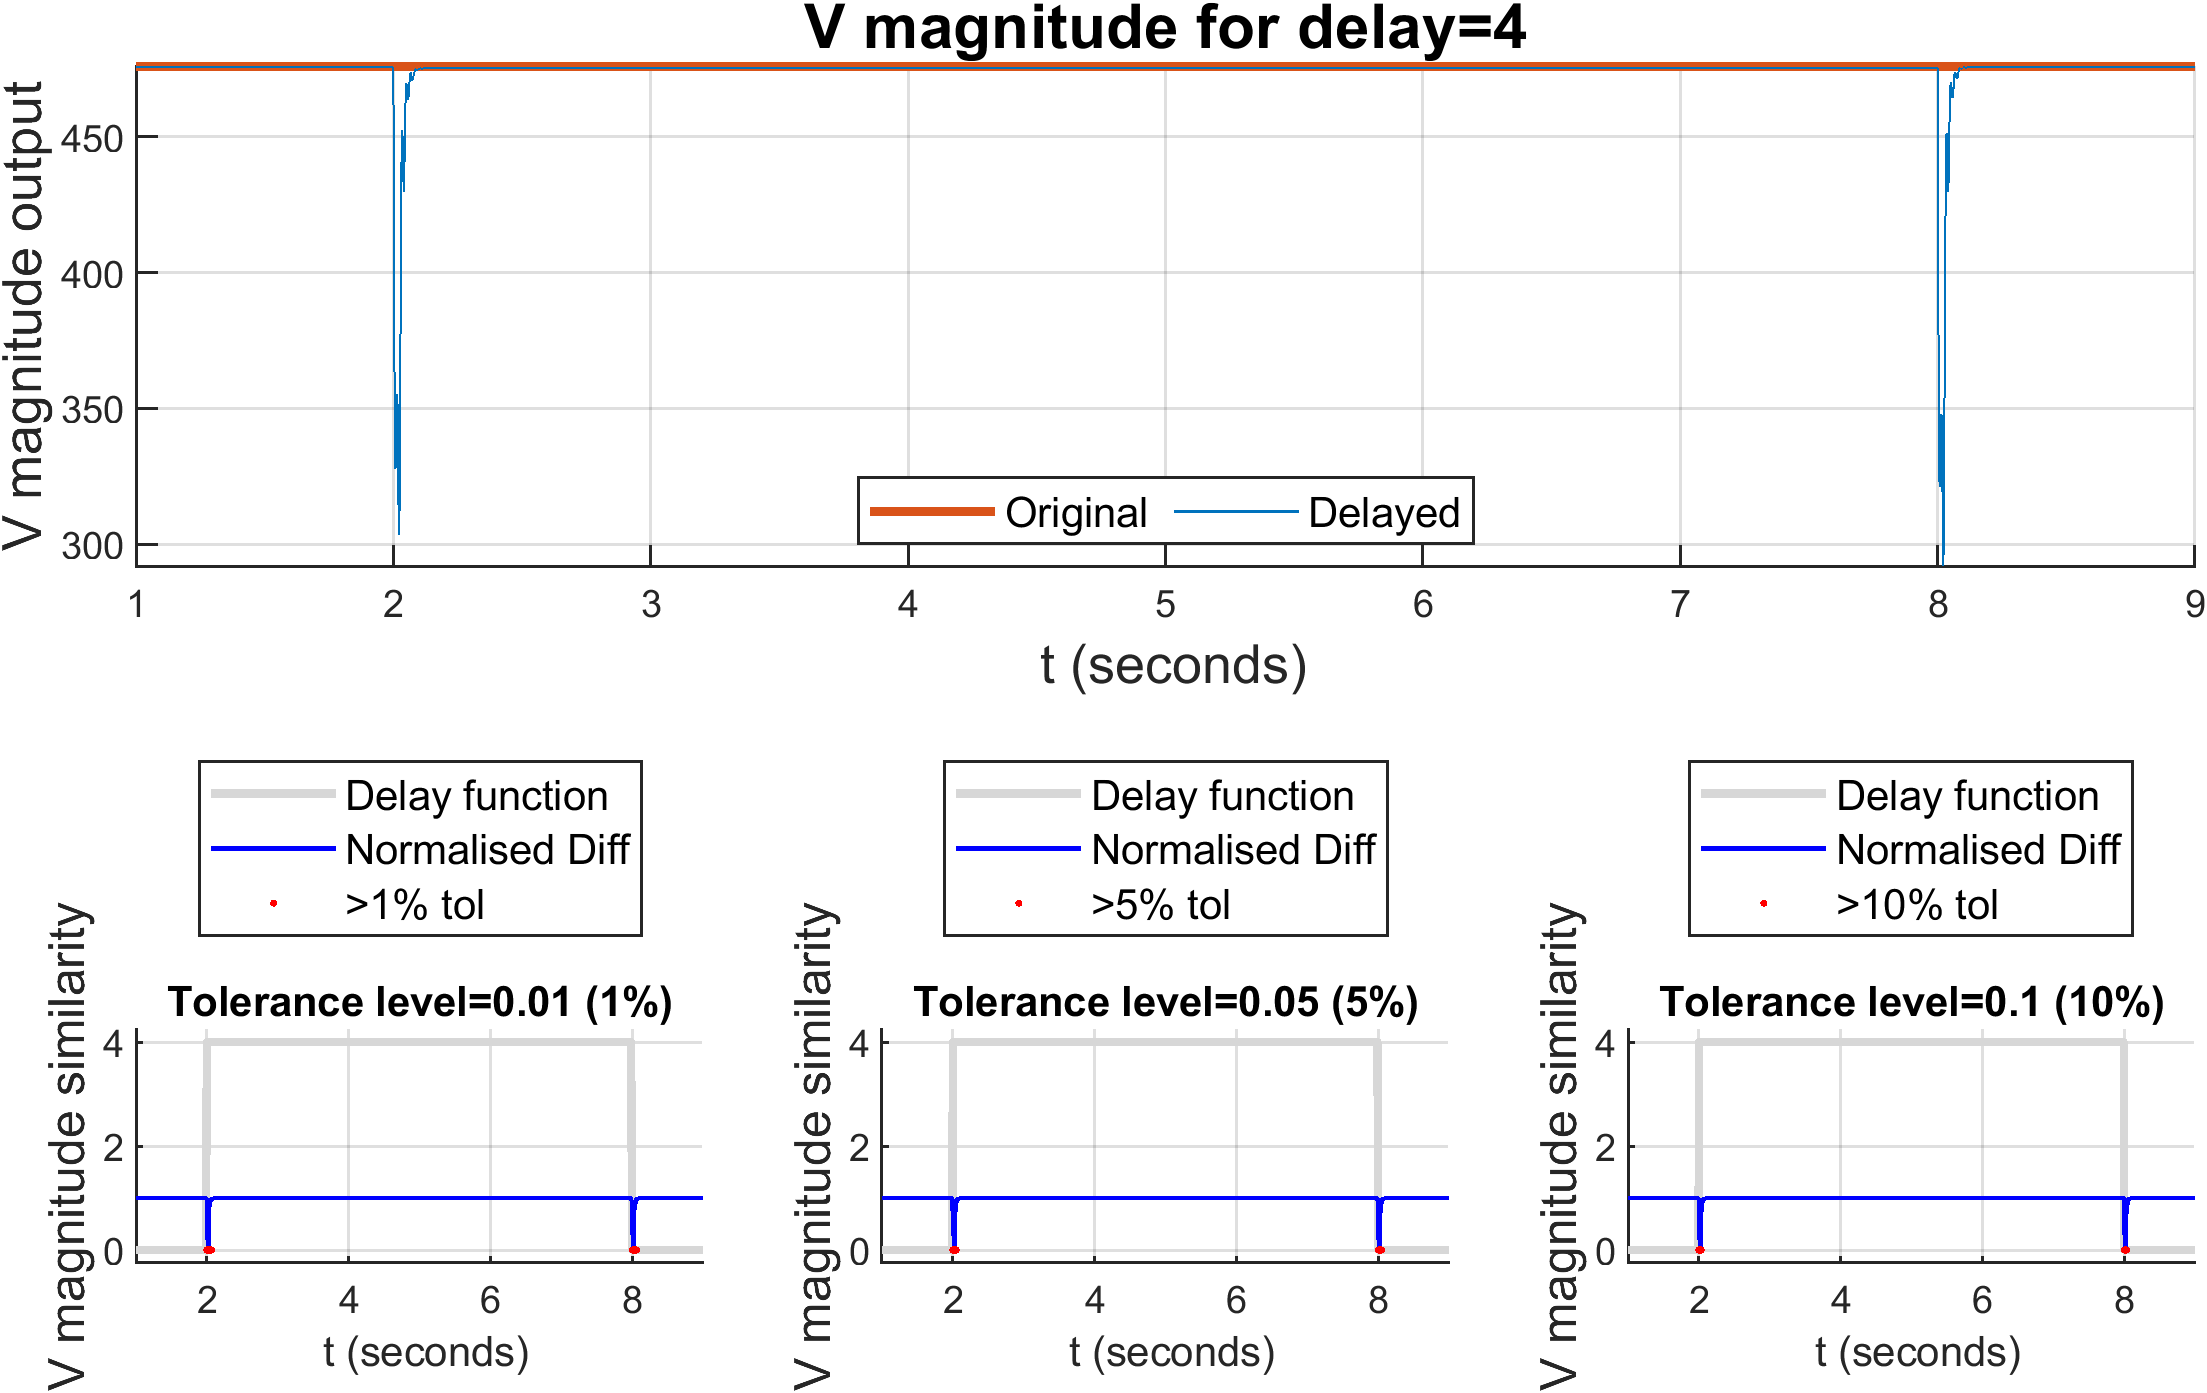
\includegraphics[width=0.95\textwidth]{PMUsim-figures/DelayOf_4/Instant_vMagnitude.png}    
      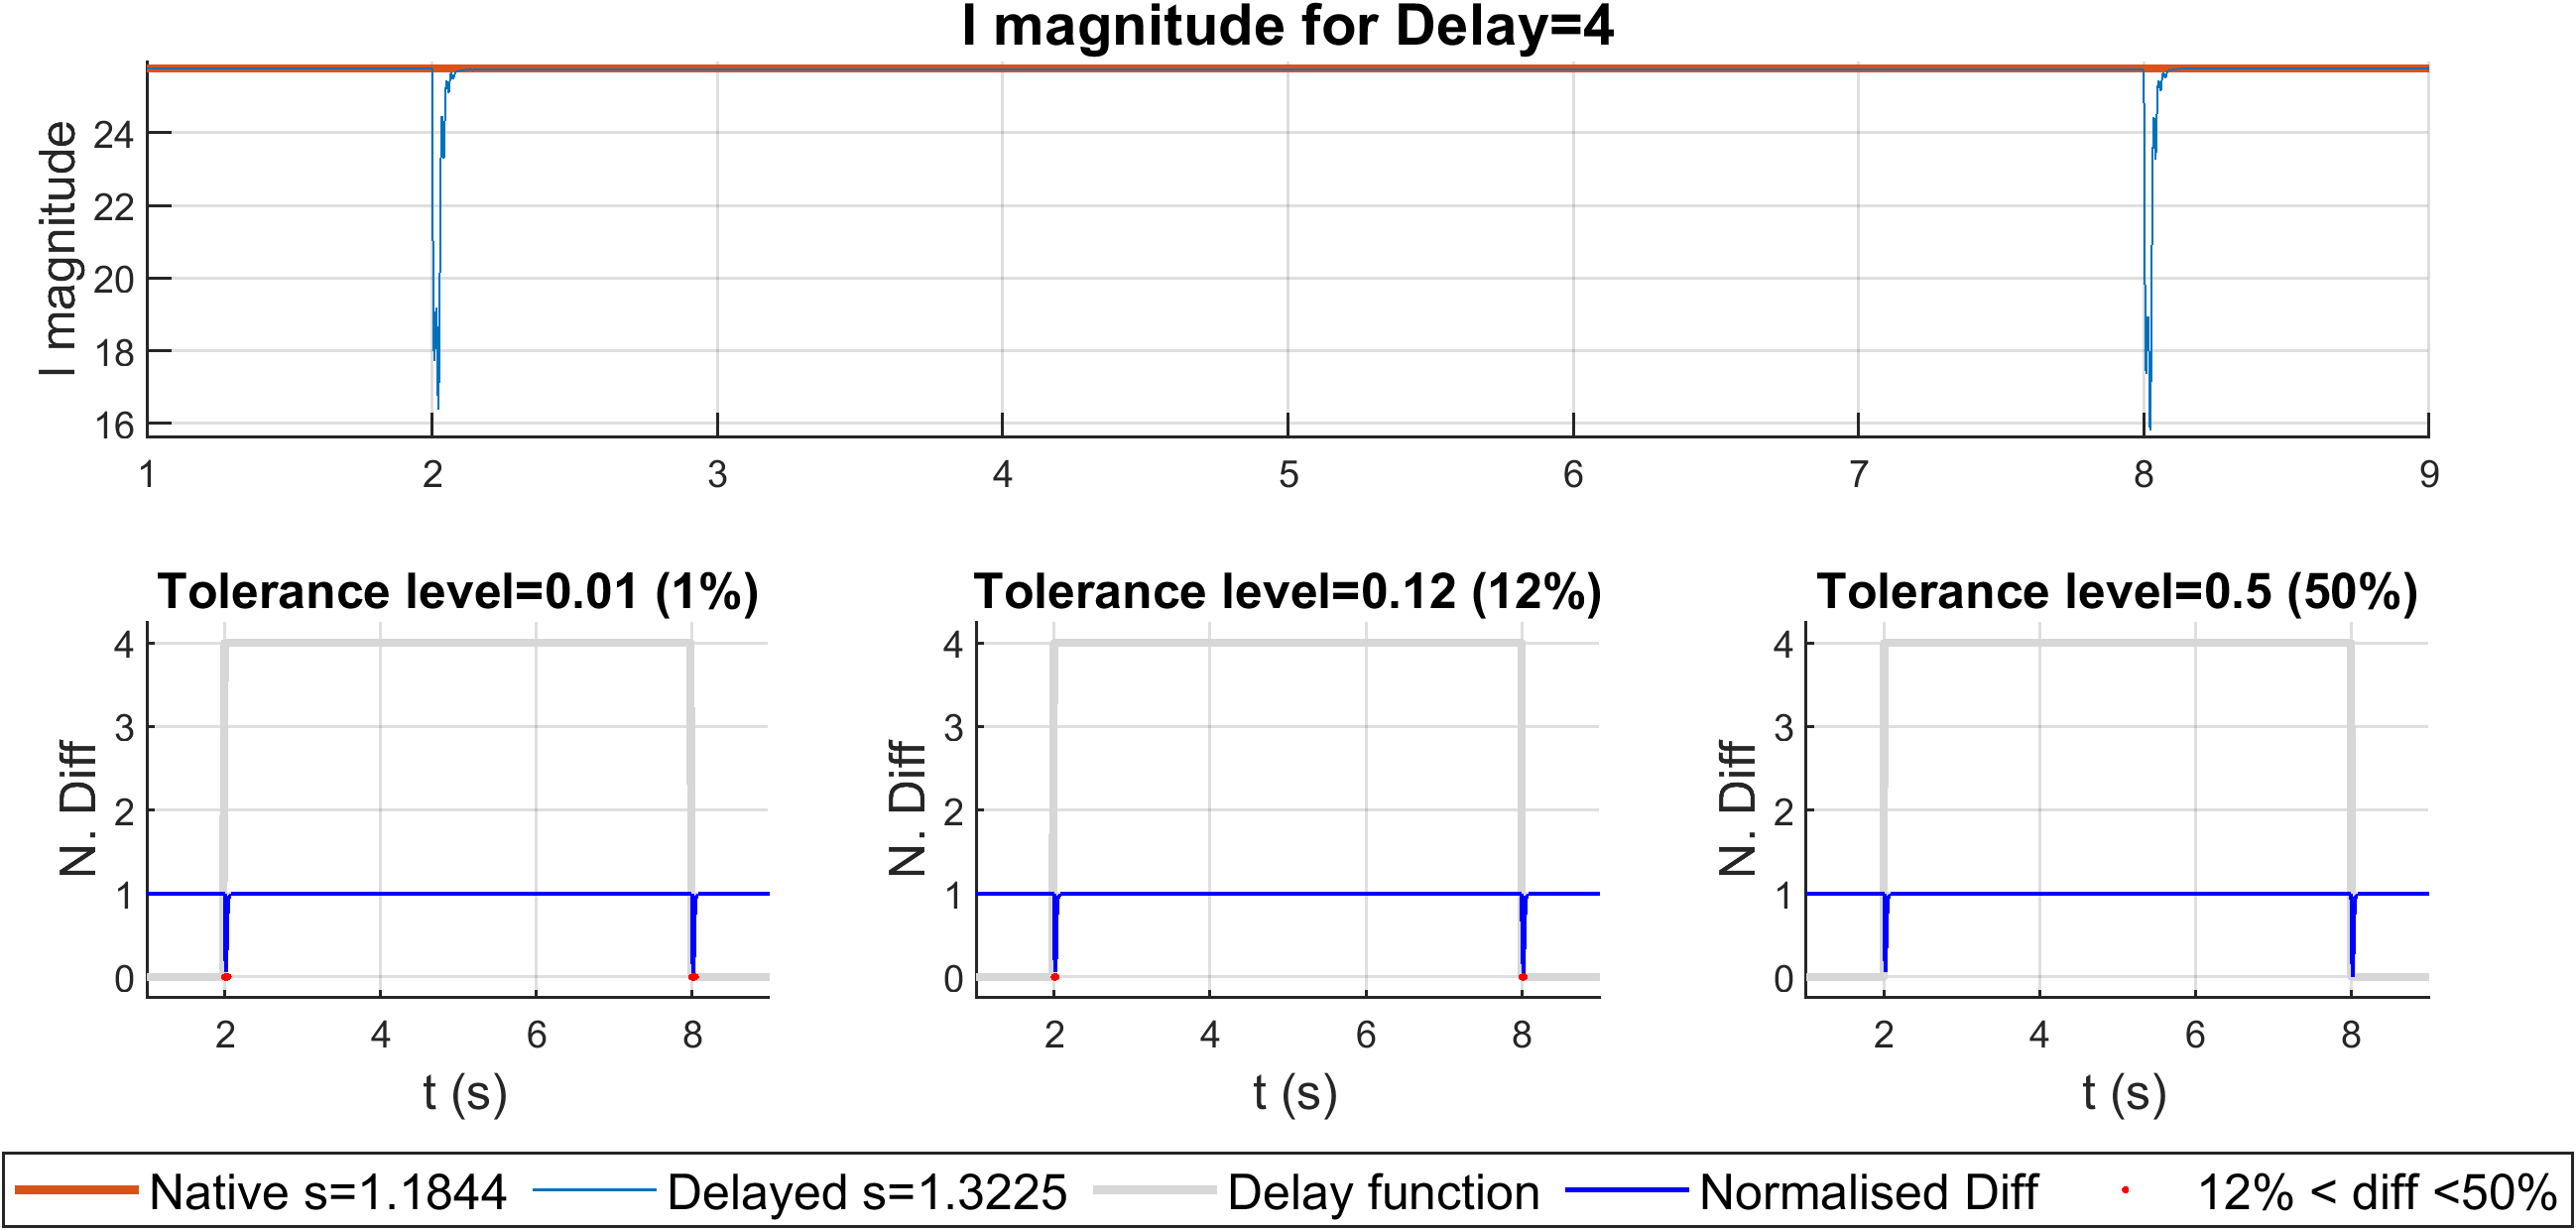
\includegraphics[width=0.95\textwidth]{PMUsim-figures/DelayOf_4/Instant_iMagnitude.png}         \label{fig:PMUsim_Four_Magnitude}
\end{floatingfigure}
    \begin{small}
     \tcbox[size=small, standard jigsaw, opacityback=0, boxrule=0pt,halign=justify]{
           comment on the figure:}{\begin{itemize}          \item       \end{itemize} }
     \end{small}

\newpage \textbf{Results for Frequency Output}


\begin{floatingfigure}[p]{\textwidth}
    \caption{Instant Delay Frequency Output for the Delay Level of Four}
    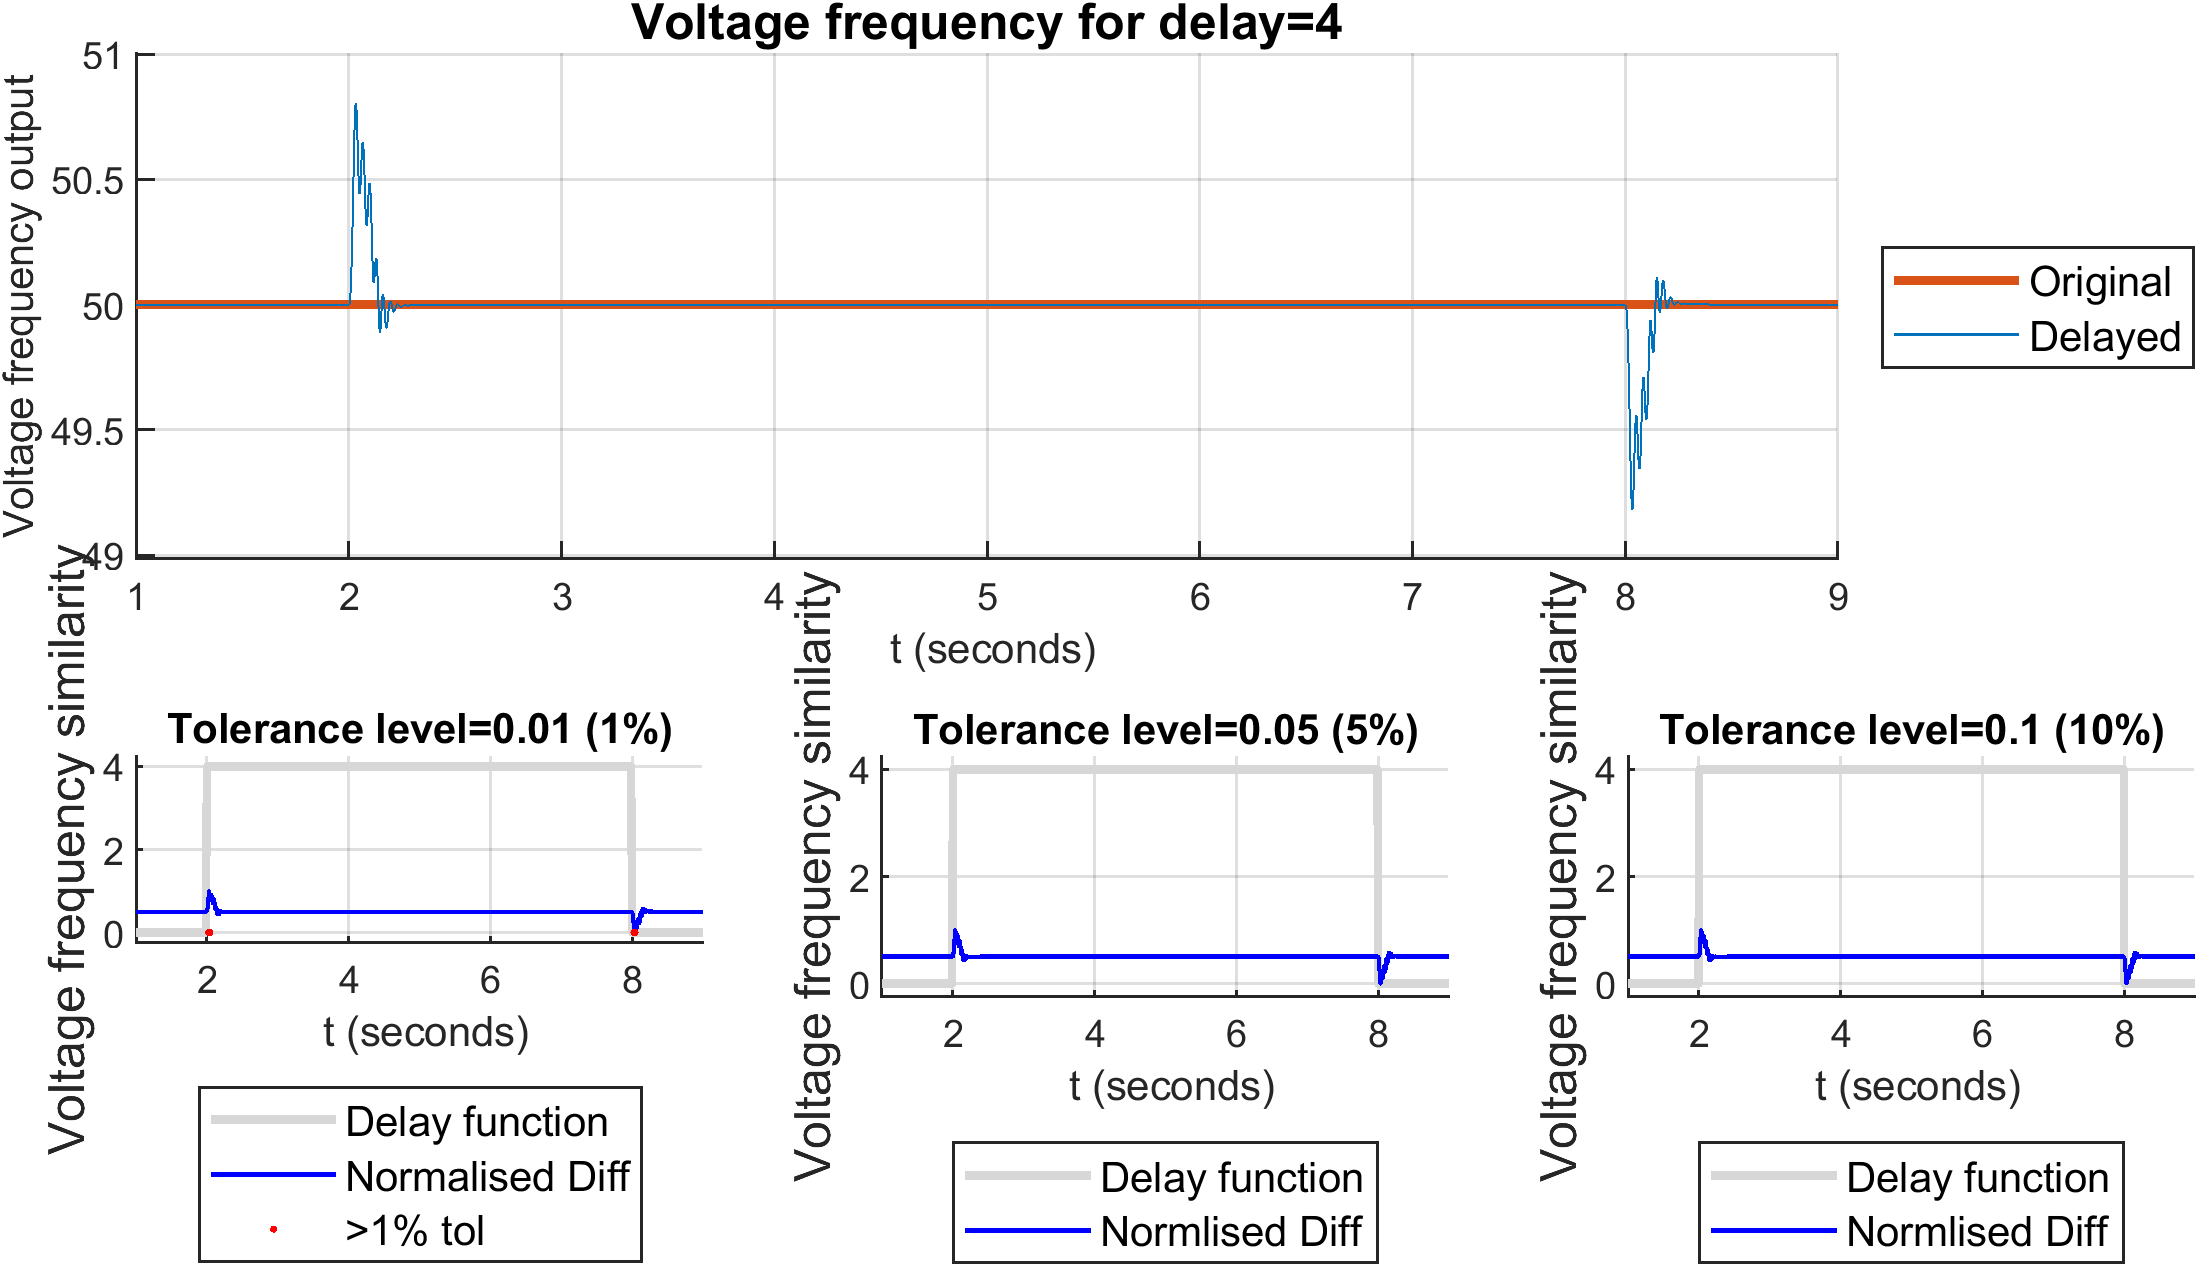
\includegraphics[width=0.95\textwidth]{PMUsim-figures/DelayOf_4/Instant_vFrequency.png}    
    \label{fig:PMUsim_Four_vFrequency}
    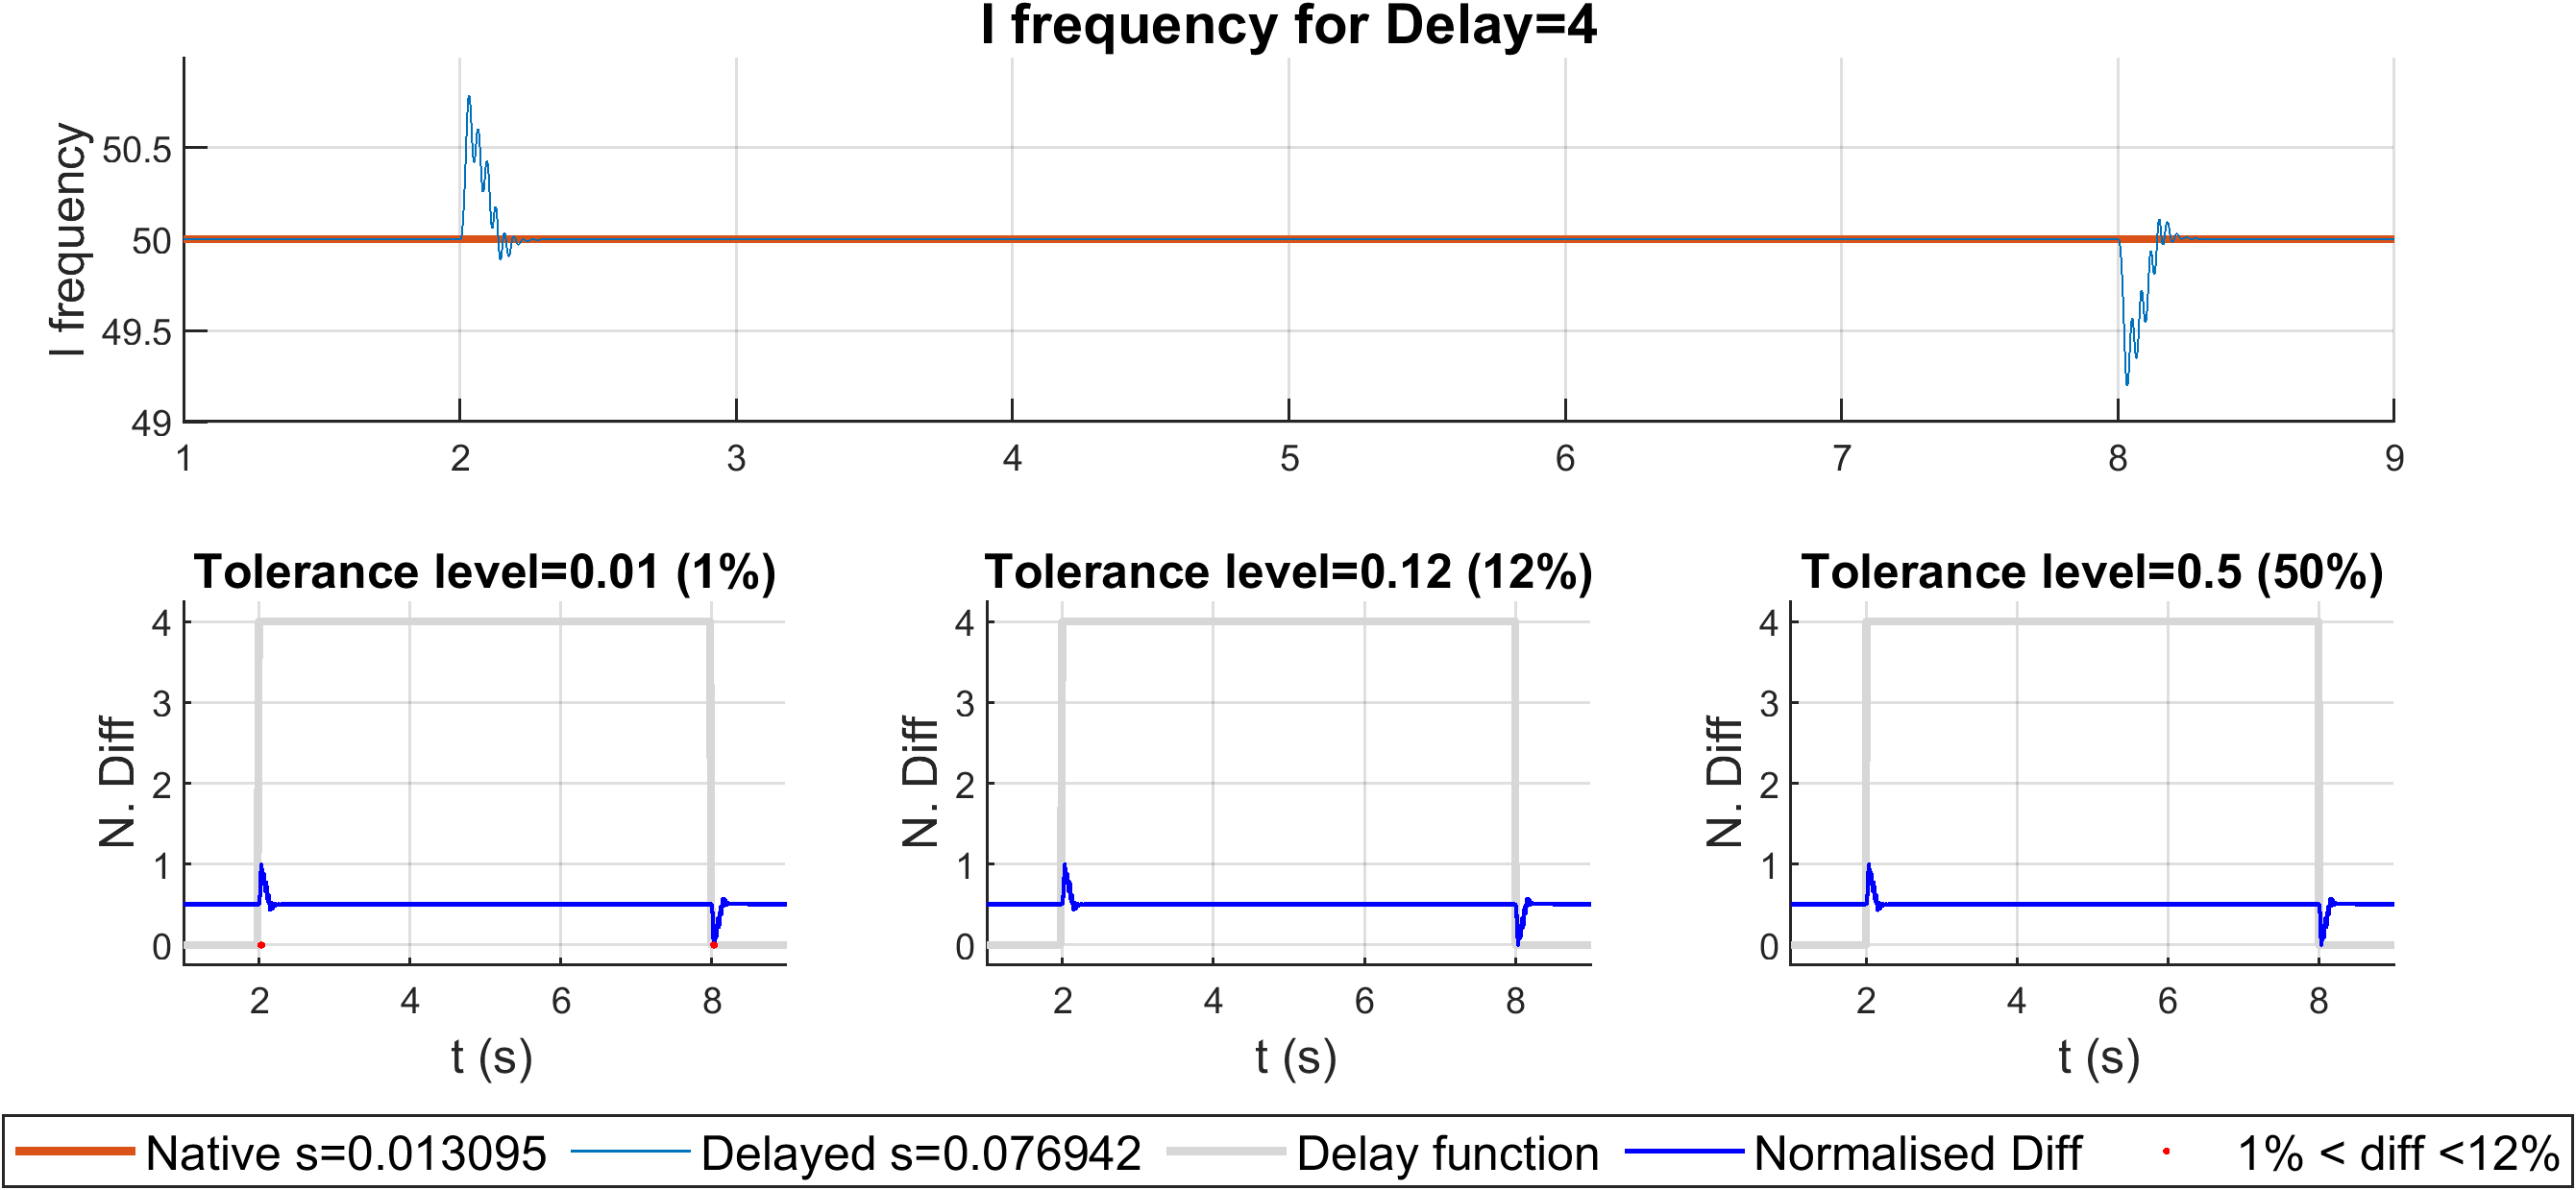
\includegraphics[width=0.95\textwidth]{PMUsim-figures/DelayOf_4/Instant_iFrequency.png}    
    \label{fig:PMUsim_Four_Frequency}
\end{floatingfigure}
        \begin{small}
     \tcbox[size=small, standard jigsaw, opacityback=0, boxrule=0pt,halign=justify]{
     Comment on the figure:}{
     \begin{itemize}
         \item 
     \end{itemize} }
     \end{small}


\newpage \textbf{Results for Angle Output}


\begin{floatingfigure}[p]{\textwidth}
    \caption{Instant Delay Angle Output for the Delay Level of Four}
    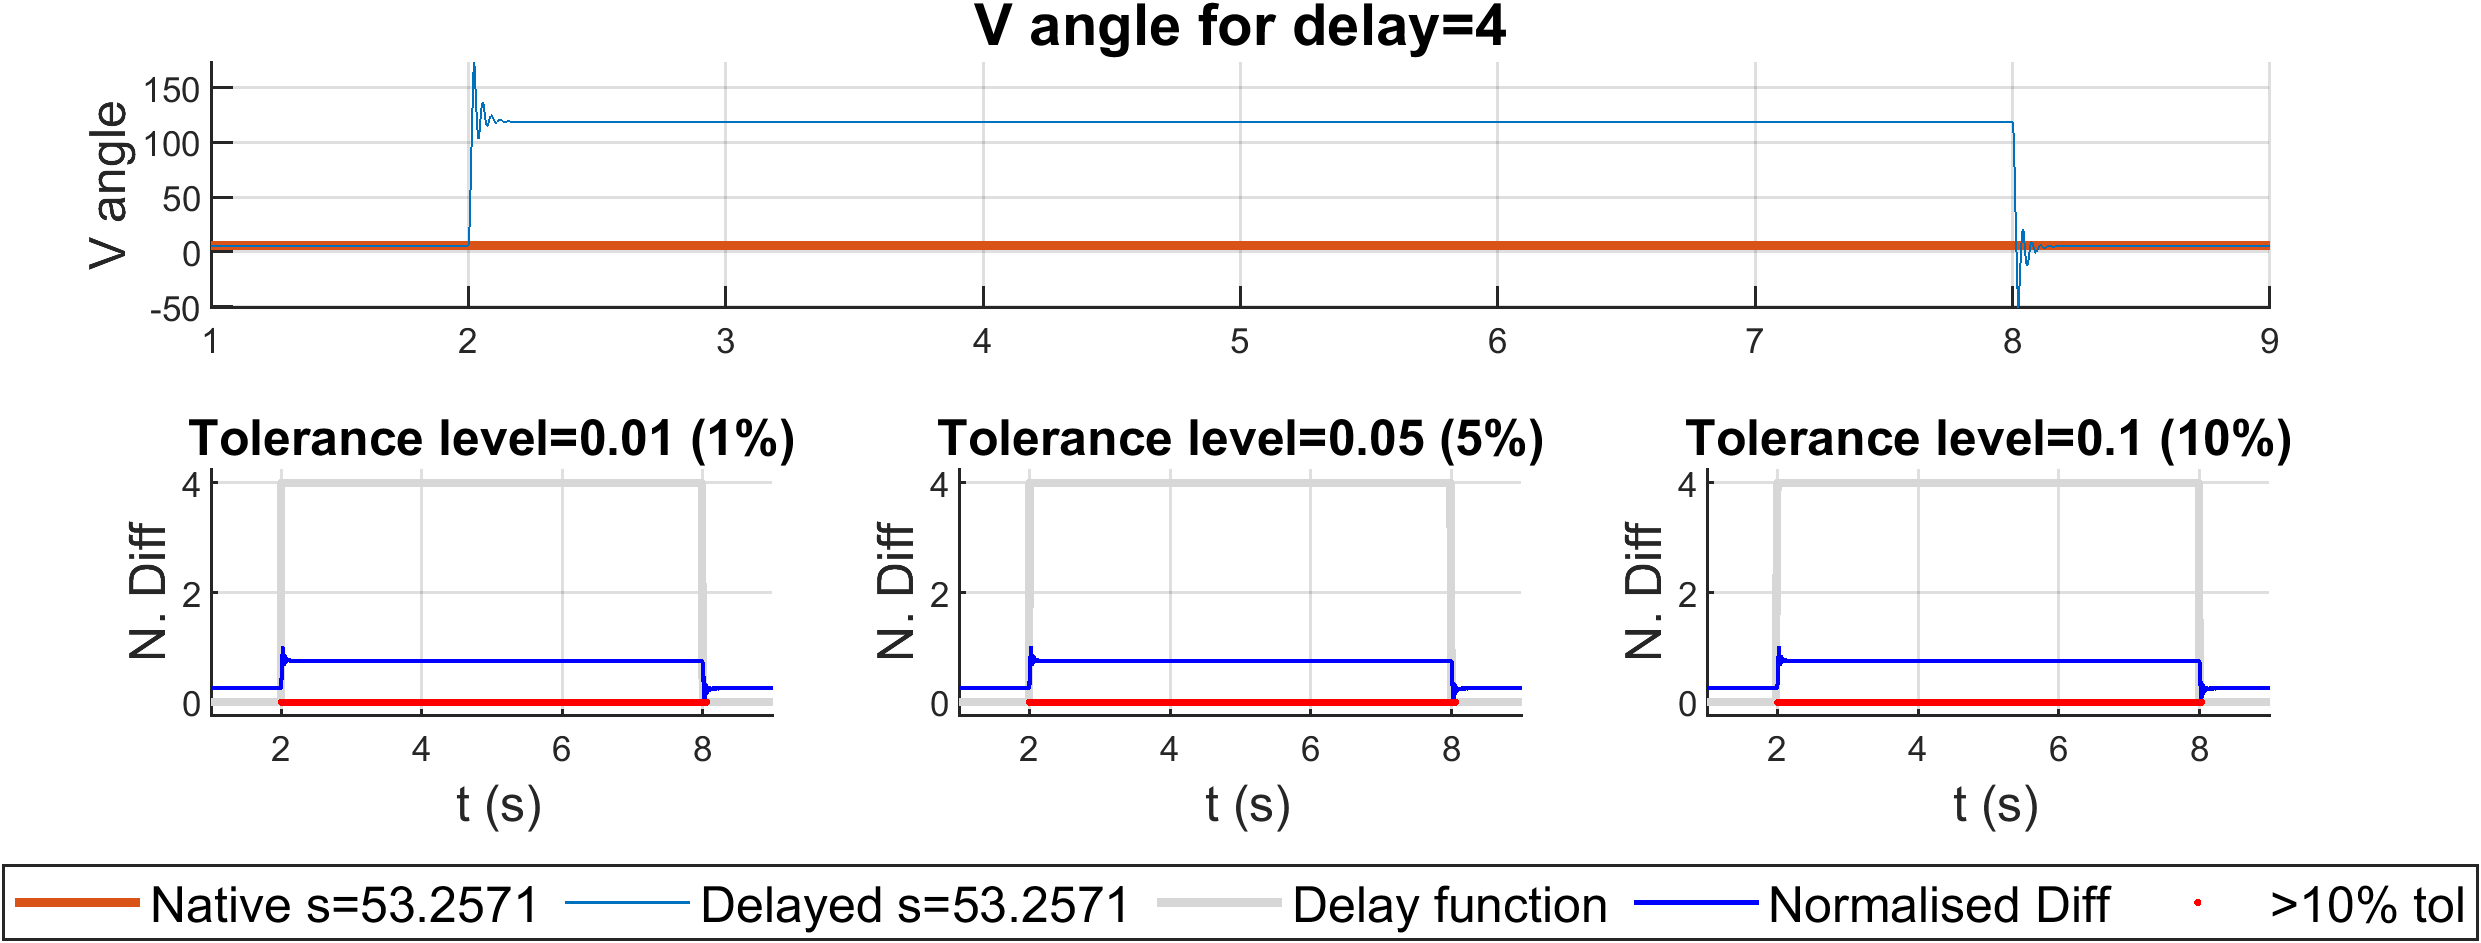
\includegraphics[width=0.95\textwidth]{PMUsim-figures/DelayOf_4/Instant_vAngle.png}    
   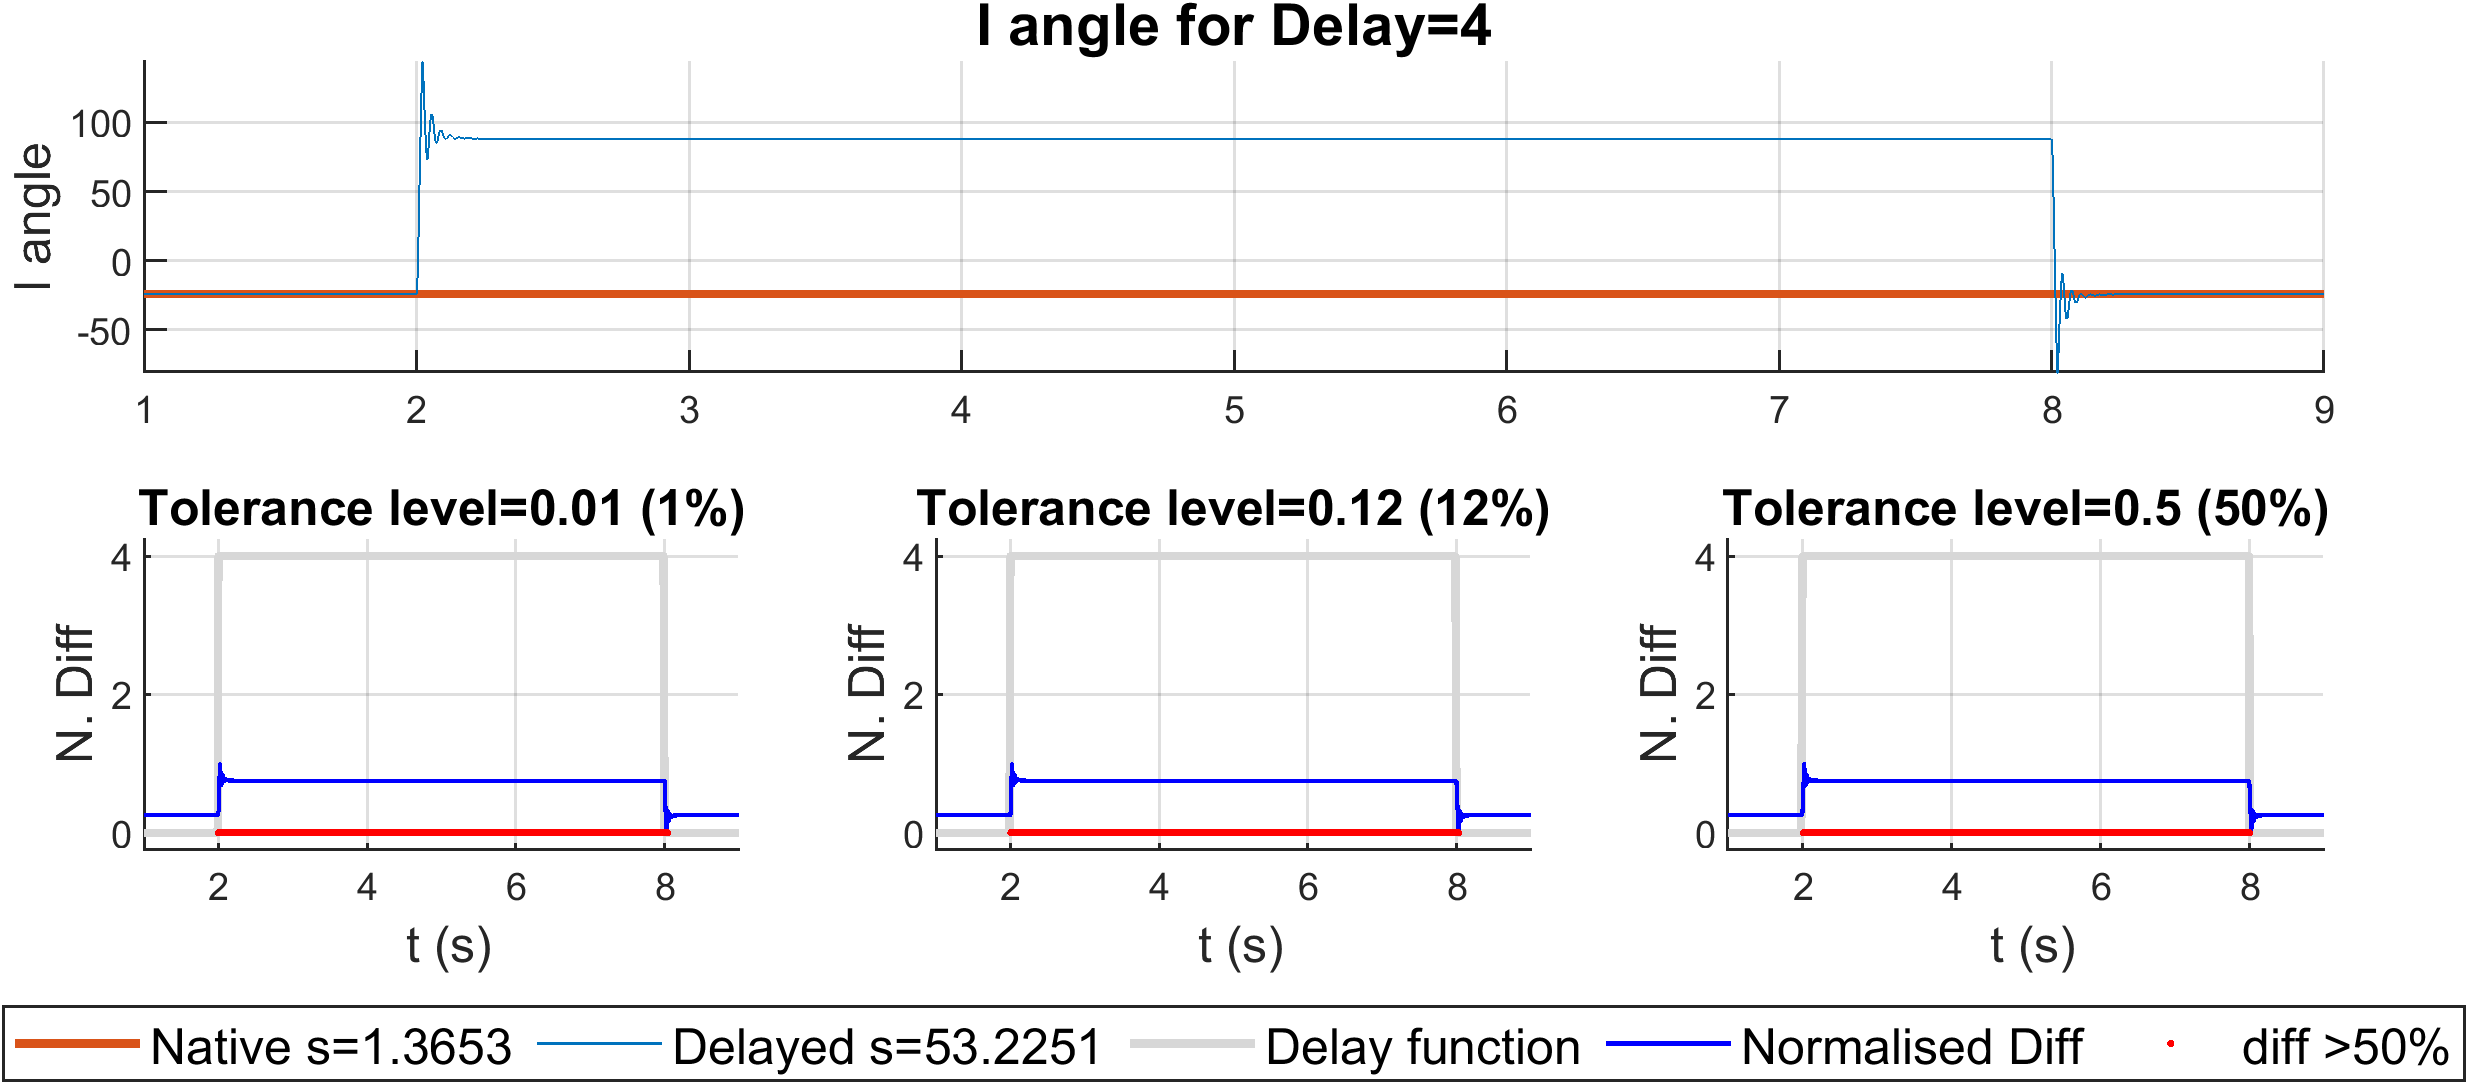
\includegraphics[width=0.95\textwidth]{PMUsim-figures/DelayOf_4/Instant_iAngle.png}    
    \label{fig:PMUsim_Four_Angle}
\end{floatingfigure}
        \begin{small}
     \tcbox[size=small, standard jigsaw, opacityback=0, boxrule=0pt,halign=justify]{
     Comment on the figure:}{
     \begin{itemize}
         \item 
     \end{itemize} }
     \end{small}

\newpage \subsection{Delay Level of Five}
\textbf{Results for Magnitude Output}

\begin{floatingfigure}[p]{\textwidth}
    \caption{Instant Delay Magnitude Output for the Delay Level of Five}
    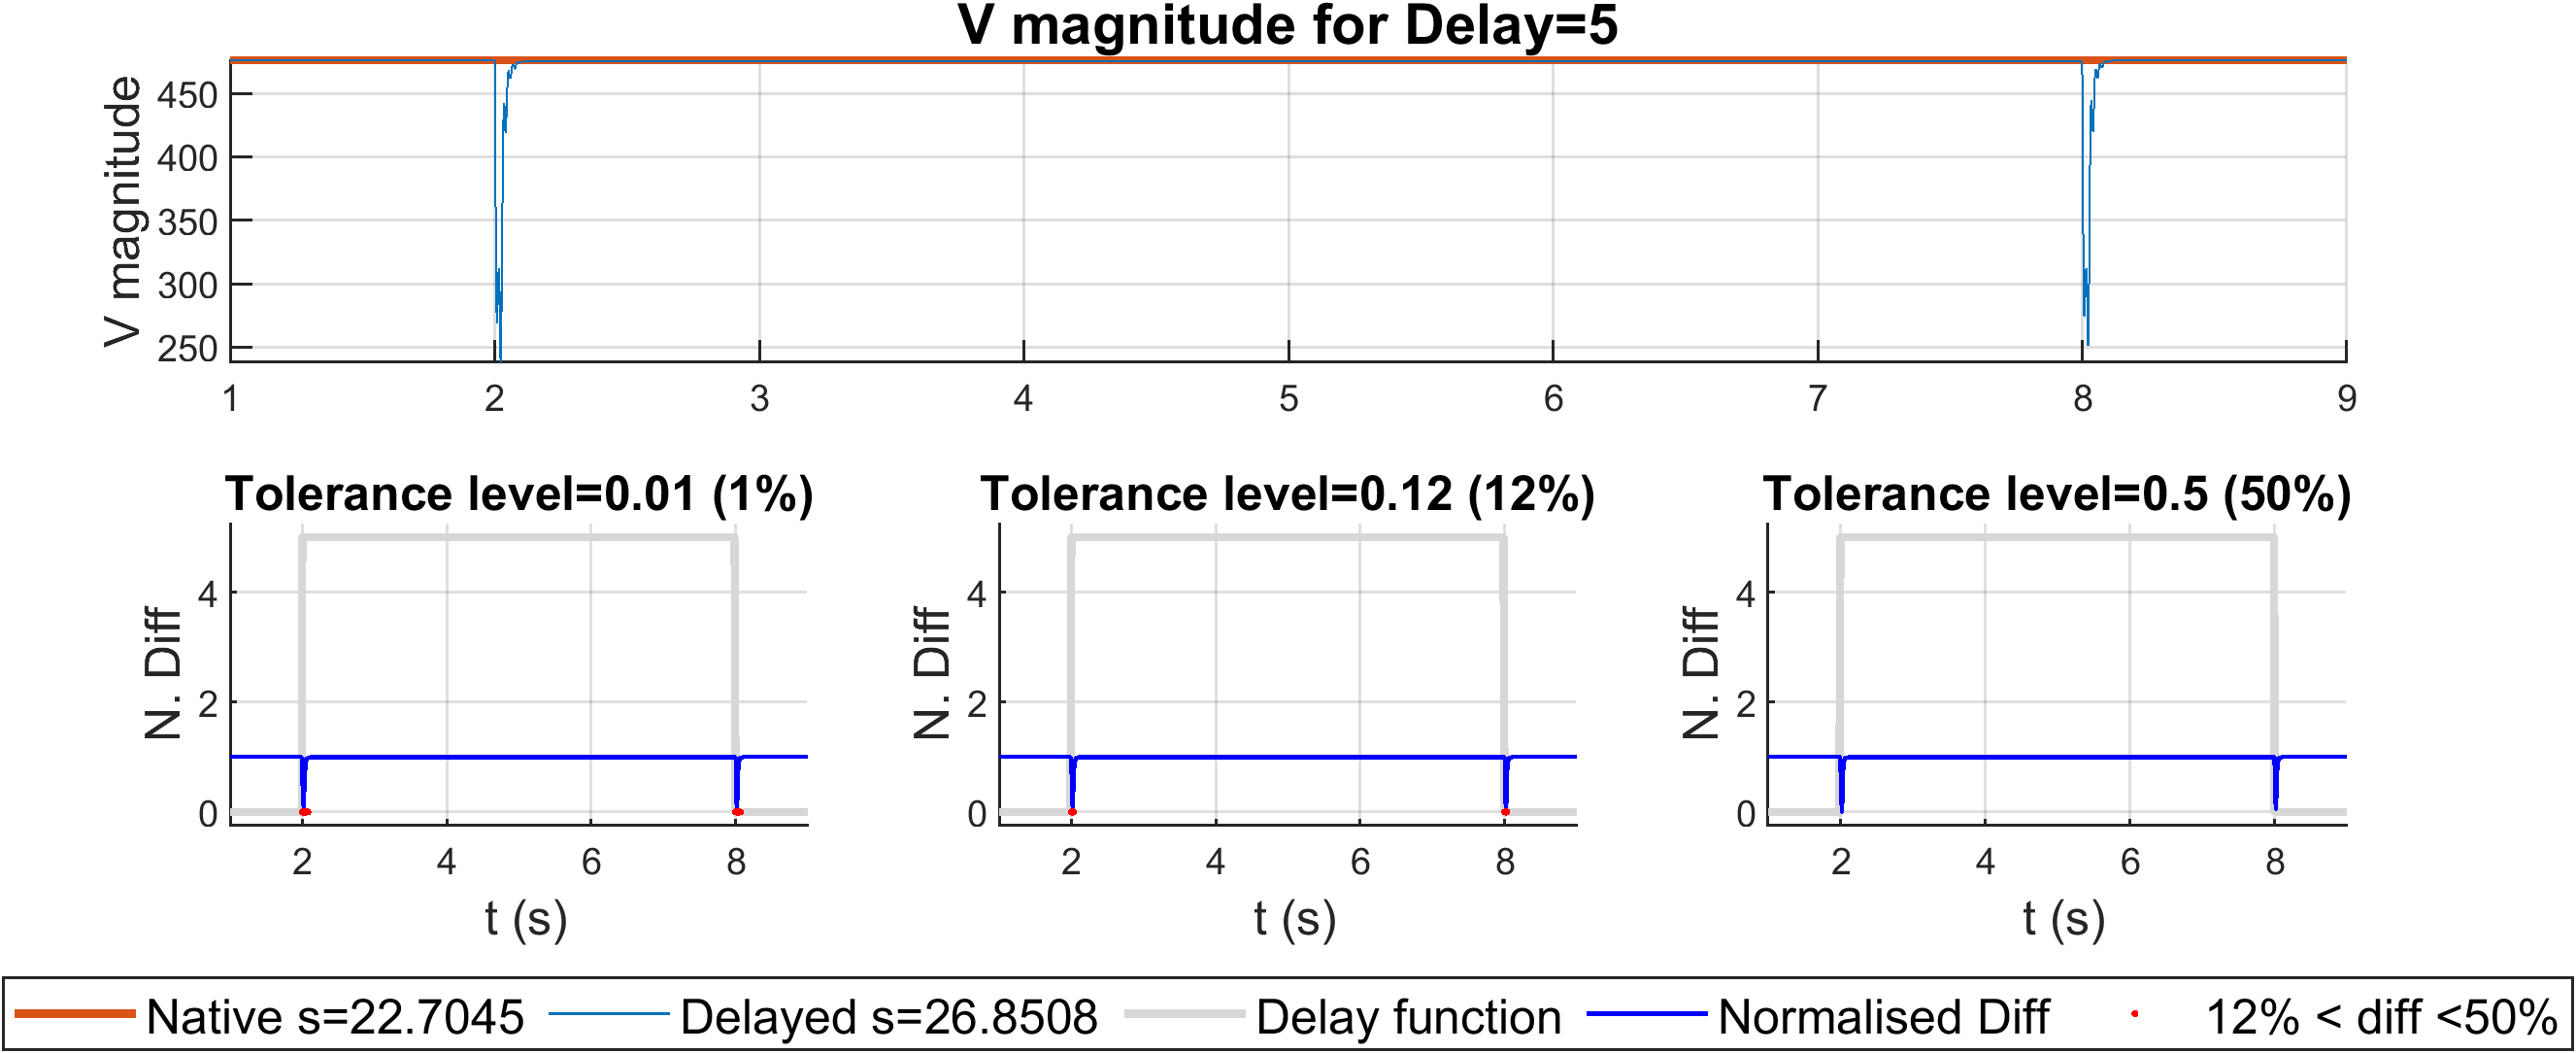
\includegraphics[width=0.95\textwidth]{PMUsim-figures/DelayOf_5/Instant_vMagnitude.png}    
      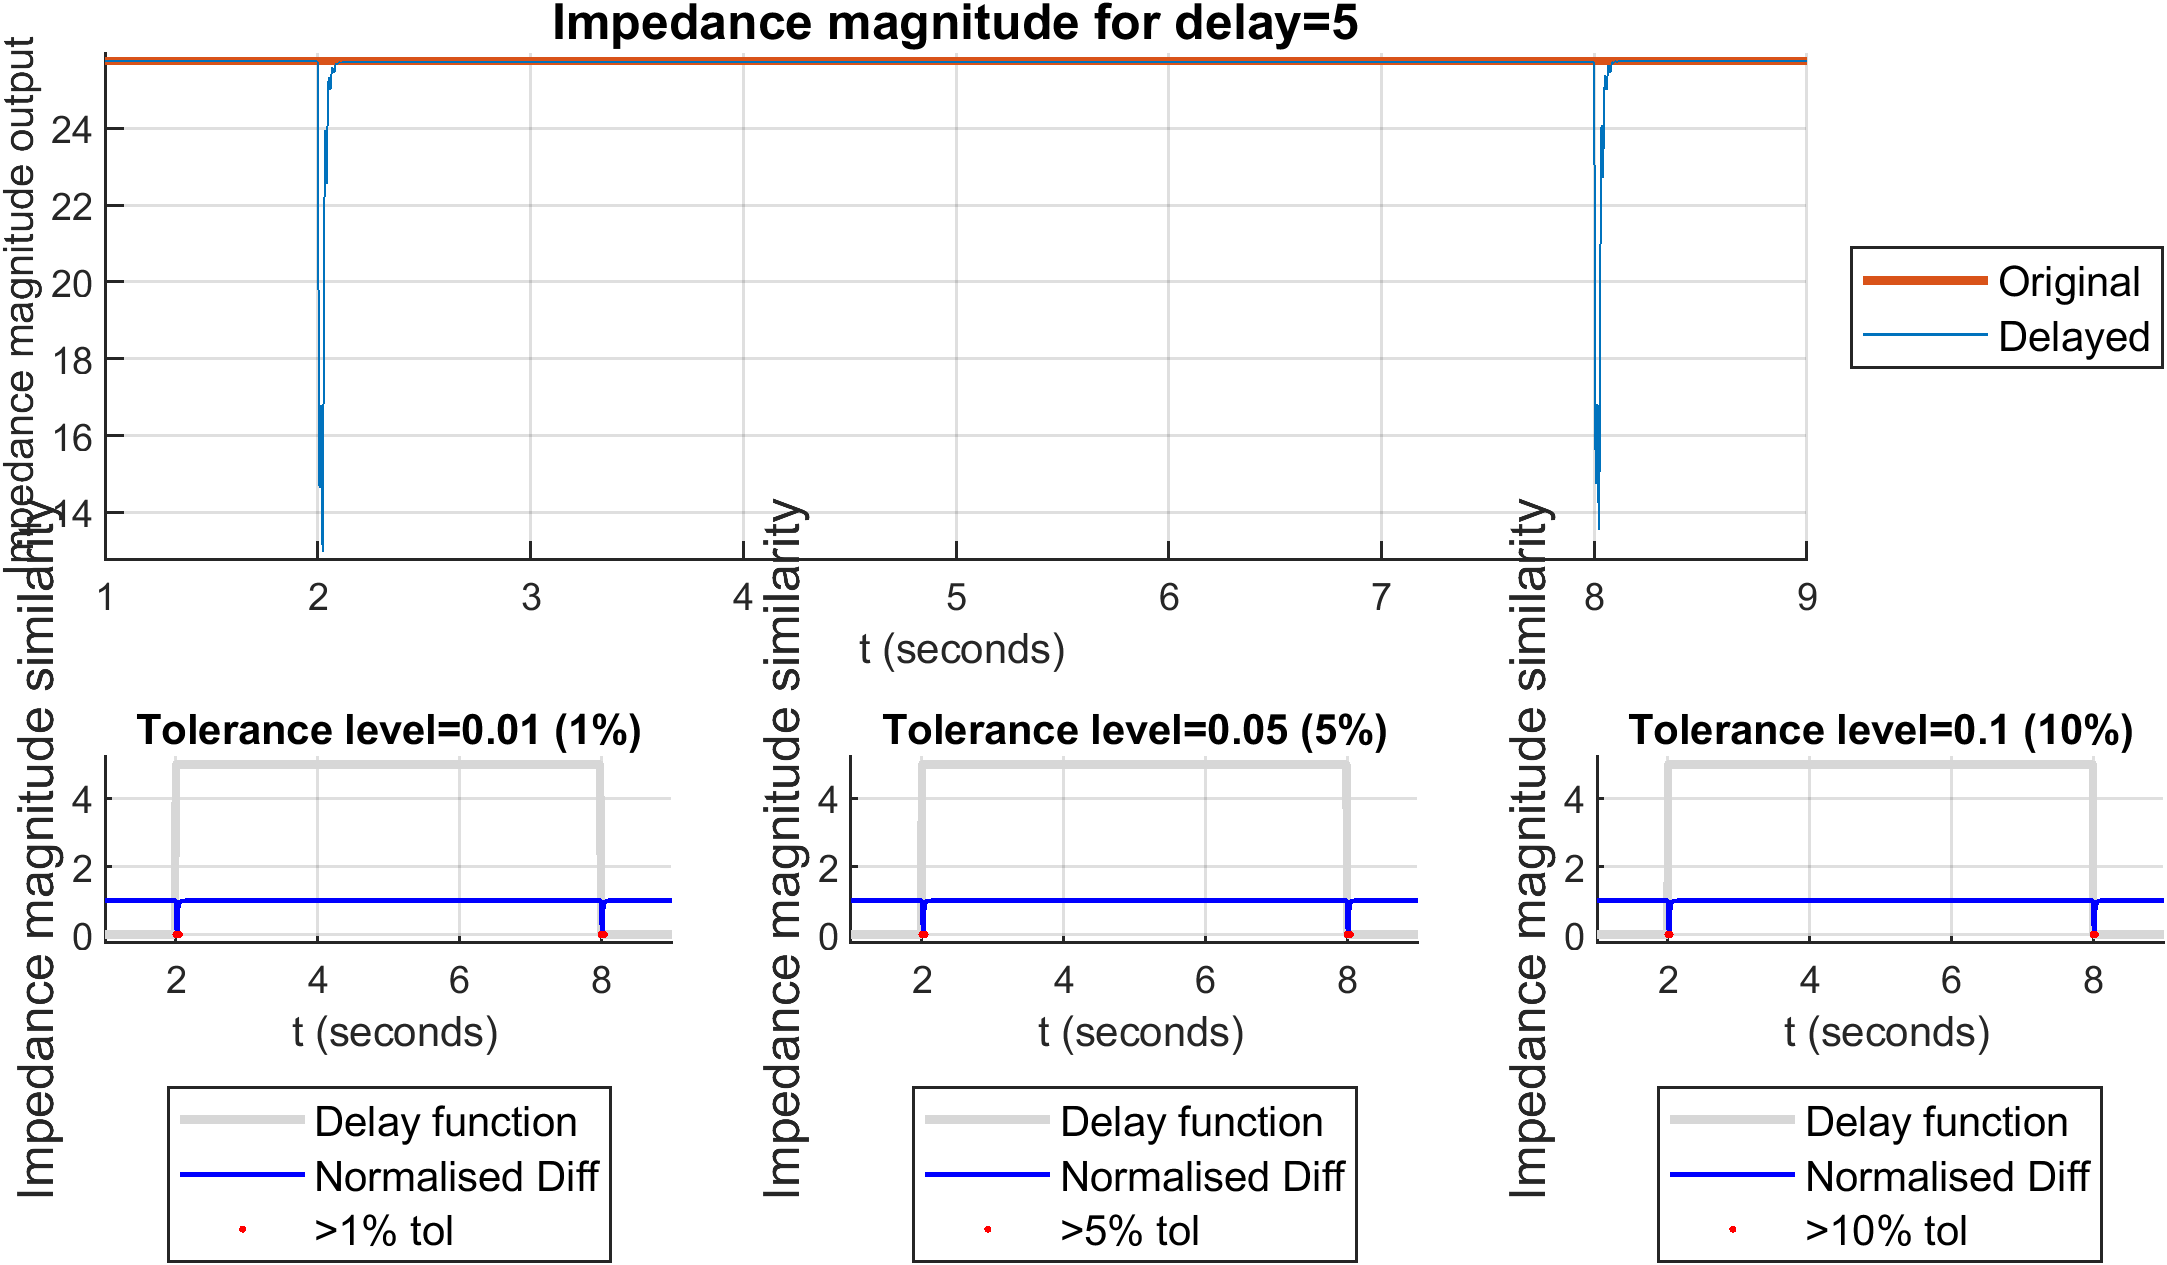
\includegraphics[width=0.95\textwidth]{PMUsim-figures/DelayOf_5/Instant_iMagnitude.png}     
    \label{fig:PMUsim_Five_Magnitude}
\end{floatingfigure}
    \begin{small}
     \tcbox[size=small, standard jigsaw, opacityback=0, boxrule=0pt,halign=justify]{
     Comment on the figure:}{
     \begin{itemize}
         \item 
     \end{itemize} }
     \end{small}

\newpage \textbf{Results for Frequency Output}


\begin{floatingfigure}[p]{\textwidth}
    \caption{Instant Delay Frequency Output for the Delay Level of Five}
    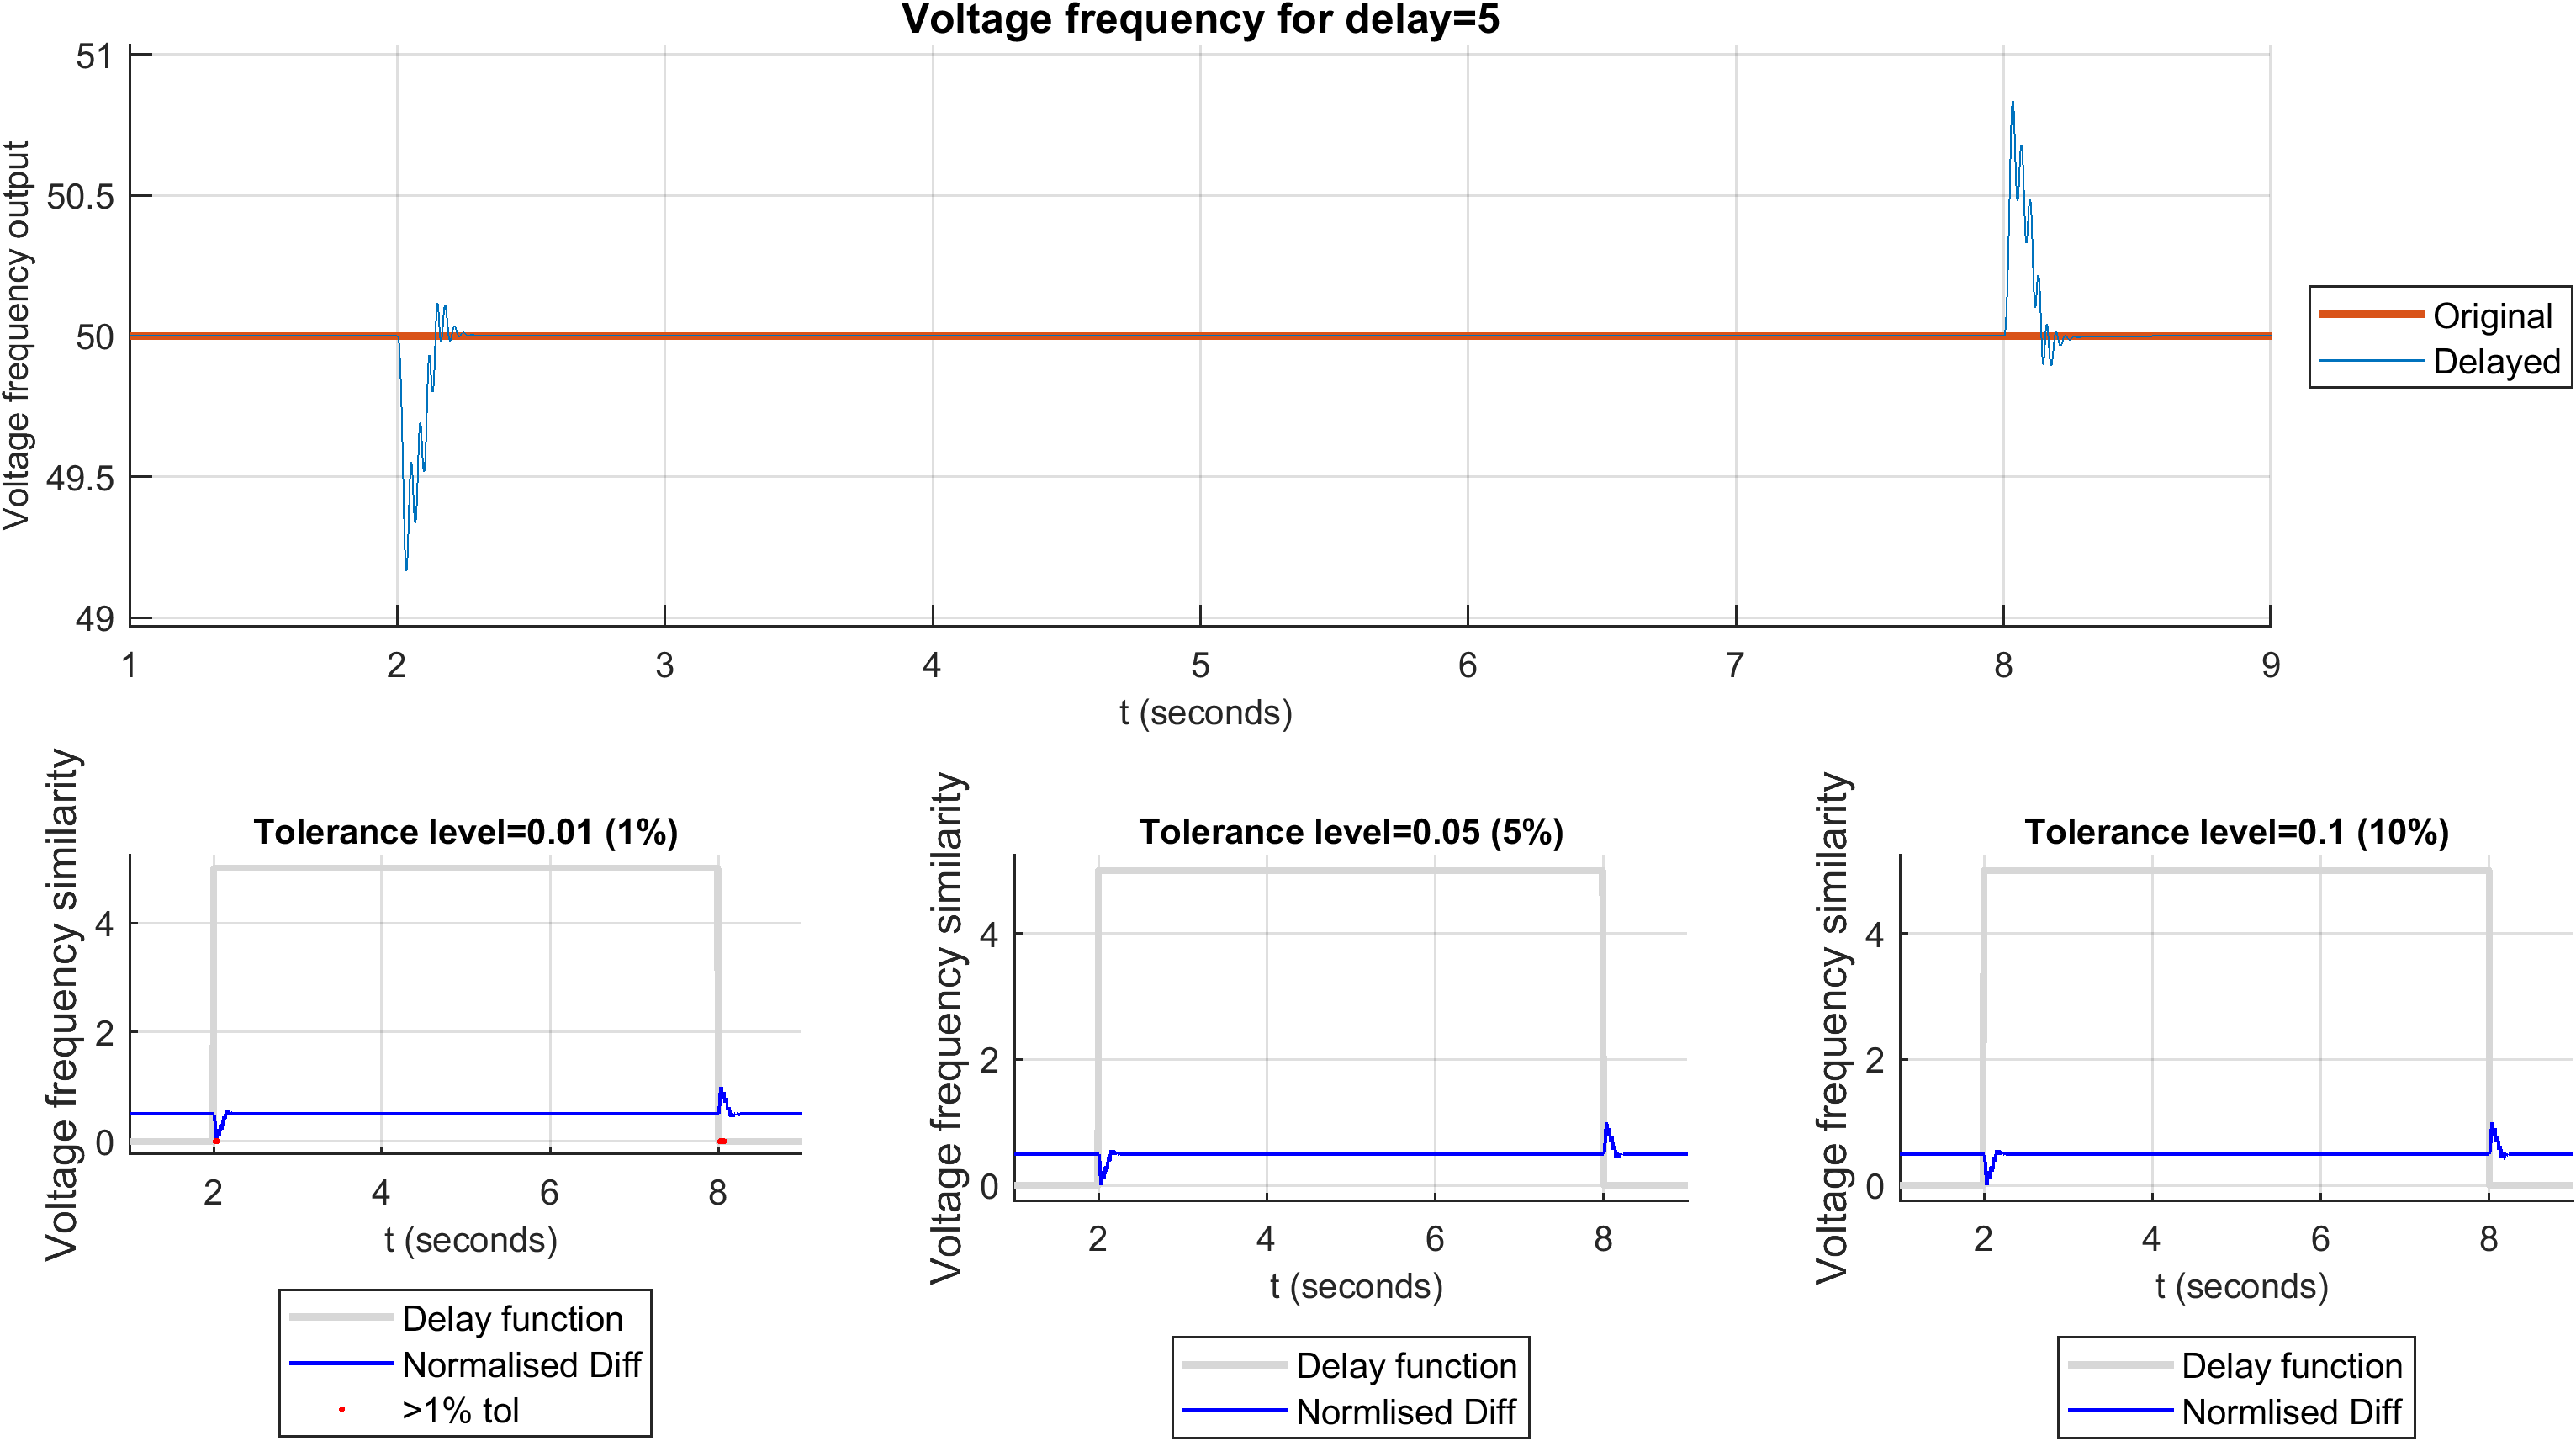
\includegraphics[width=0.95\textwidth]{PMUsim-figures/DelayOf_5/Instant_vFrequency.png}    
    \label{fig:PMUsim_Five_vFrequency}
    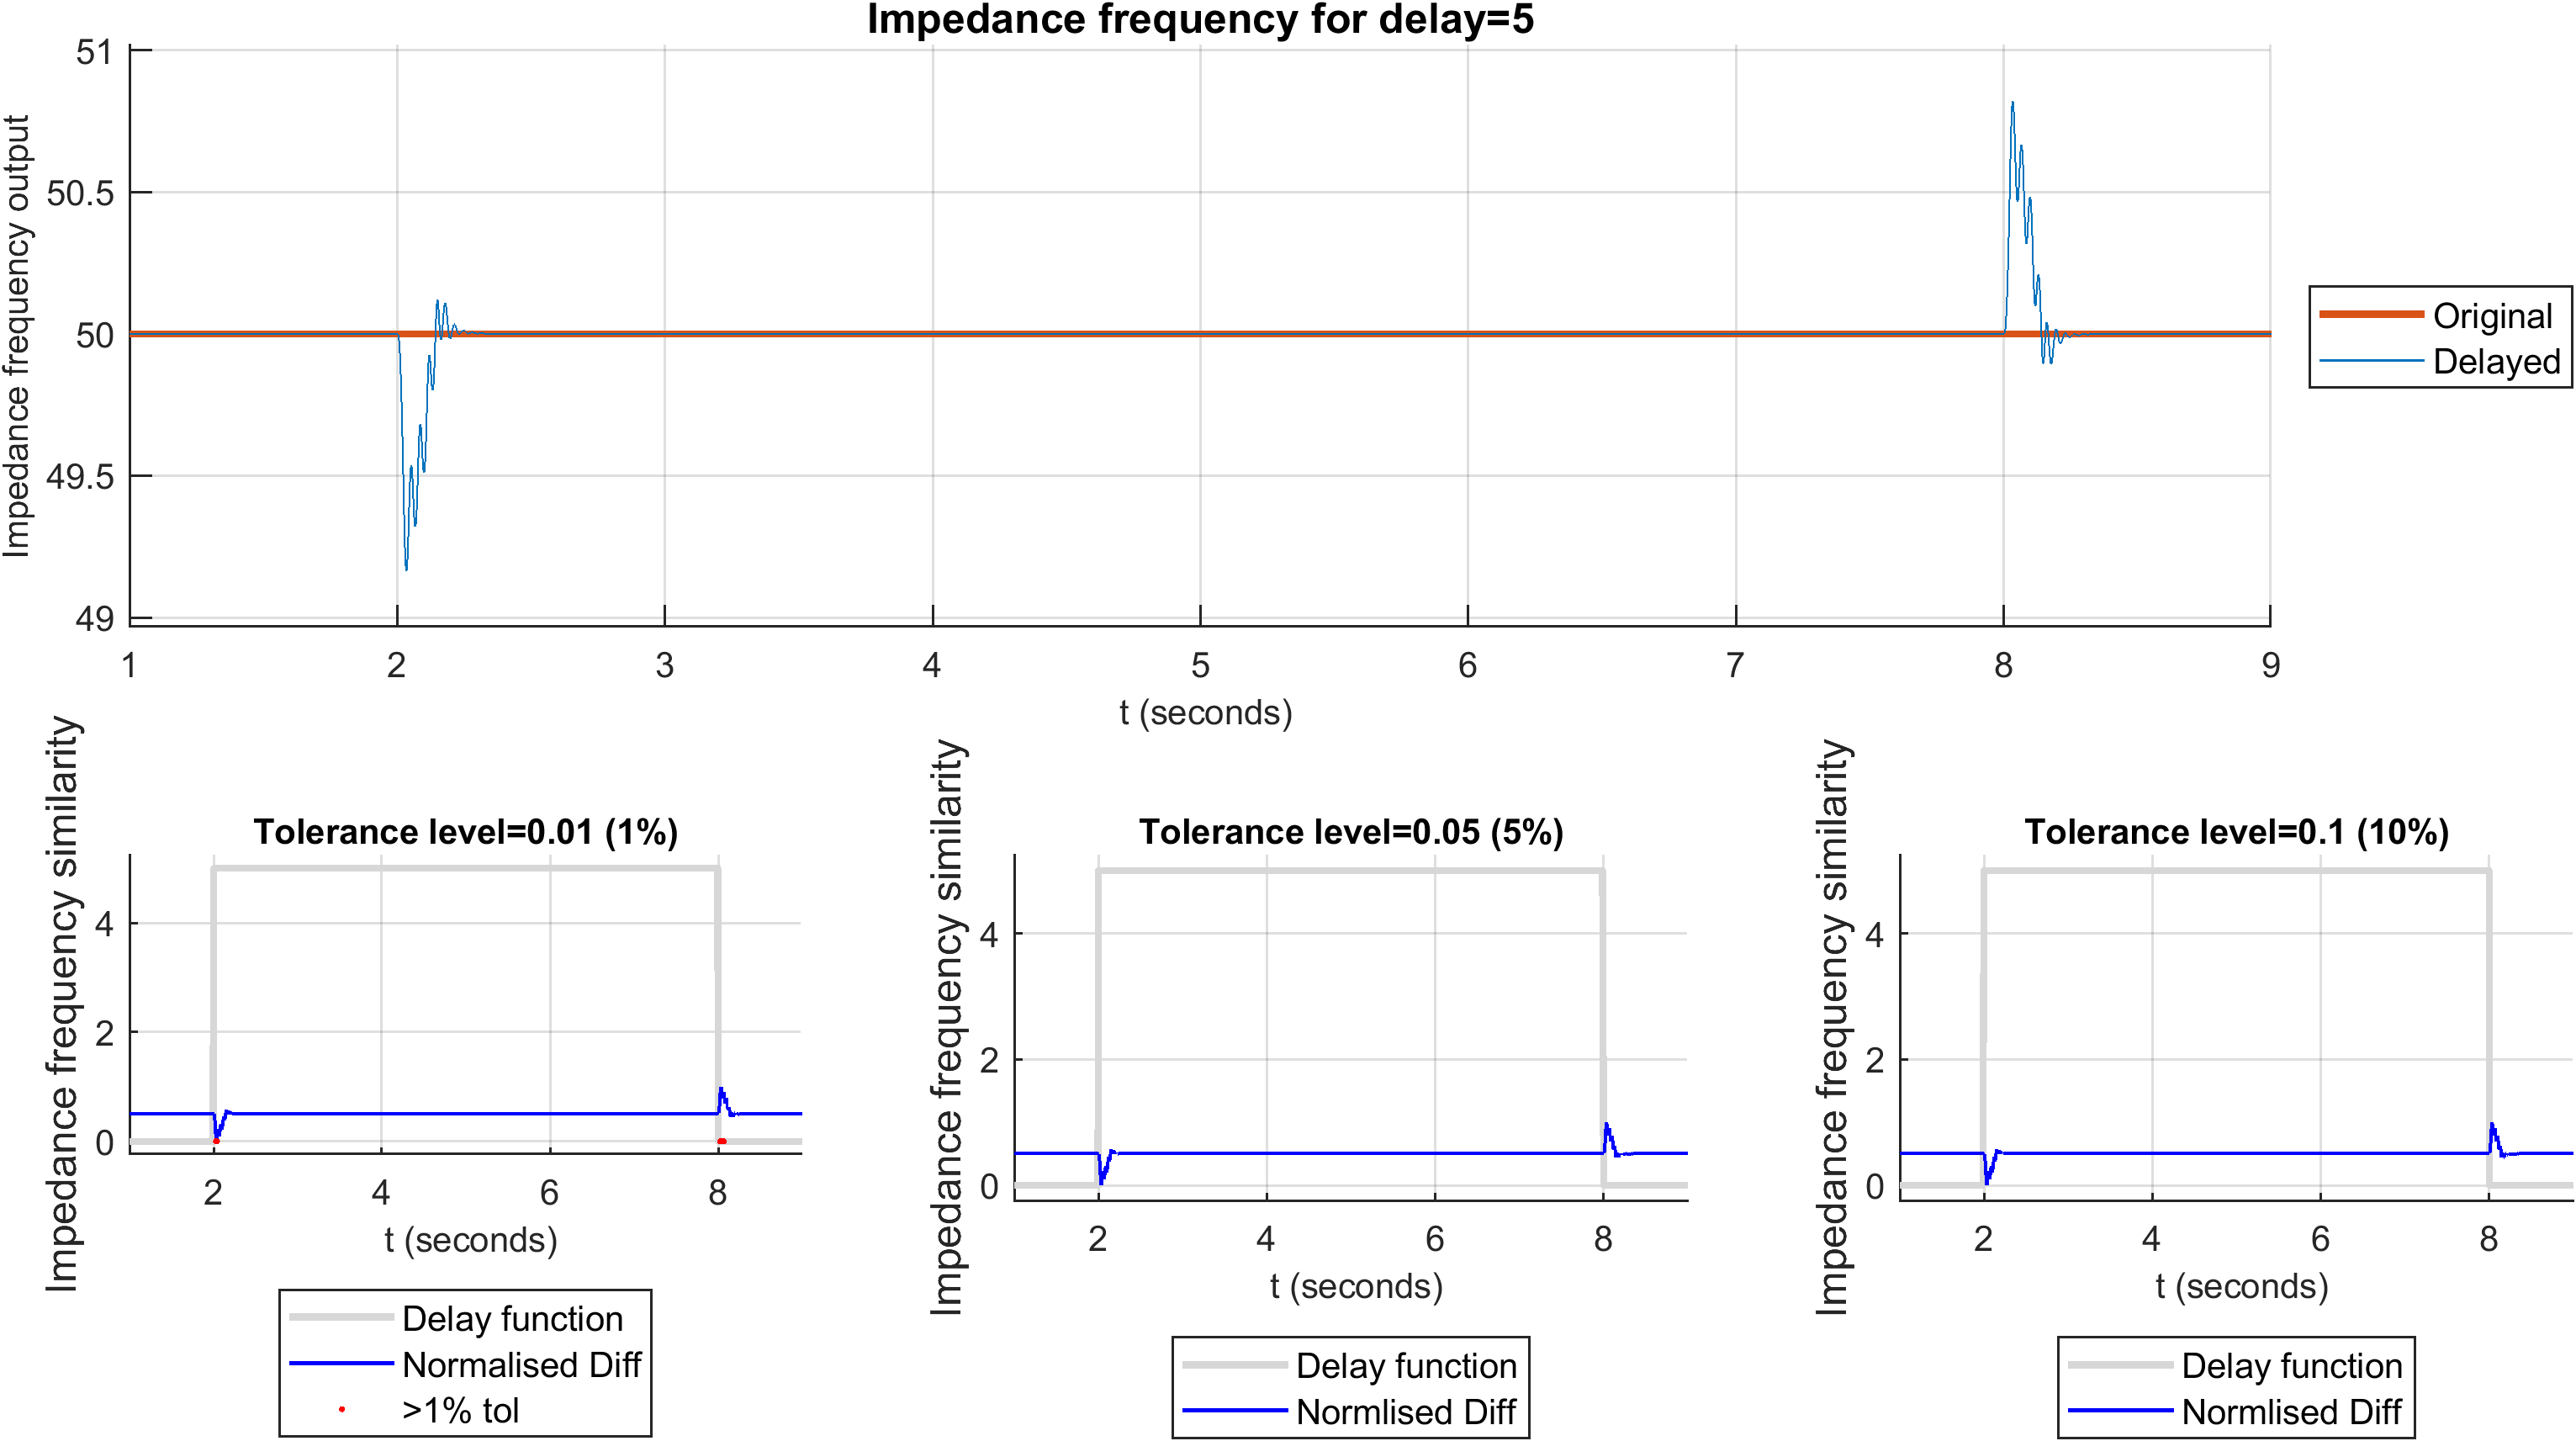
\includegraphics[width=0.95\textwidth]{PMUsim-figures/DelayOf_5/Instant_iFrequency.png}    
    \label{fig:PMUsim_Five_Frequency}
\end{floatingfigure}
        \begin{small}
     \tcbox[size=small, standard jigsaw, opacityback=0, boxrule=0pt,halign=justify]{
     Comment on the figure:}{
     \begin{itemize}
         \item 
     \end{itemize} }
     \end{small}


\newpage \textbf{Results for Angle Output}


\begin{floatingfigure}[p]{\textwidth}
    \caption{Instant Delay Angle Output for the Delay Level of Five}
    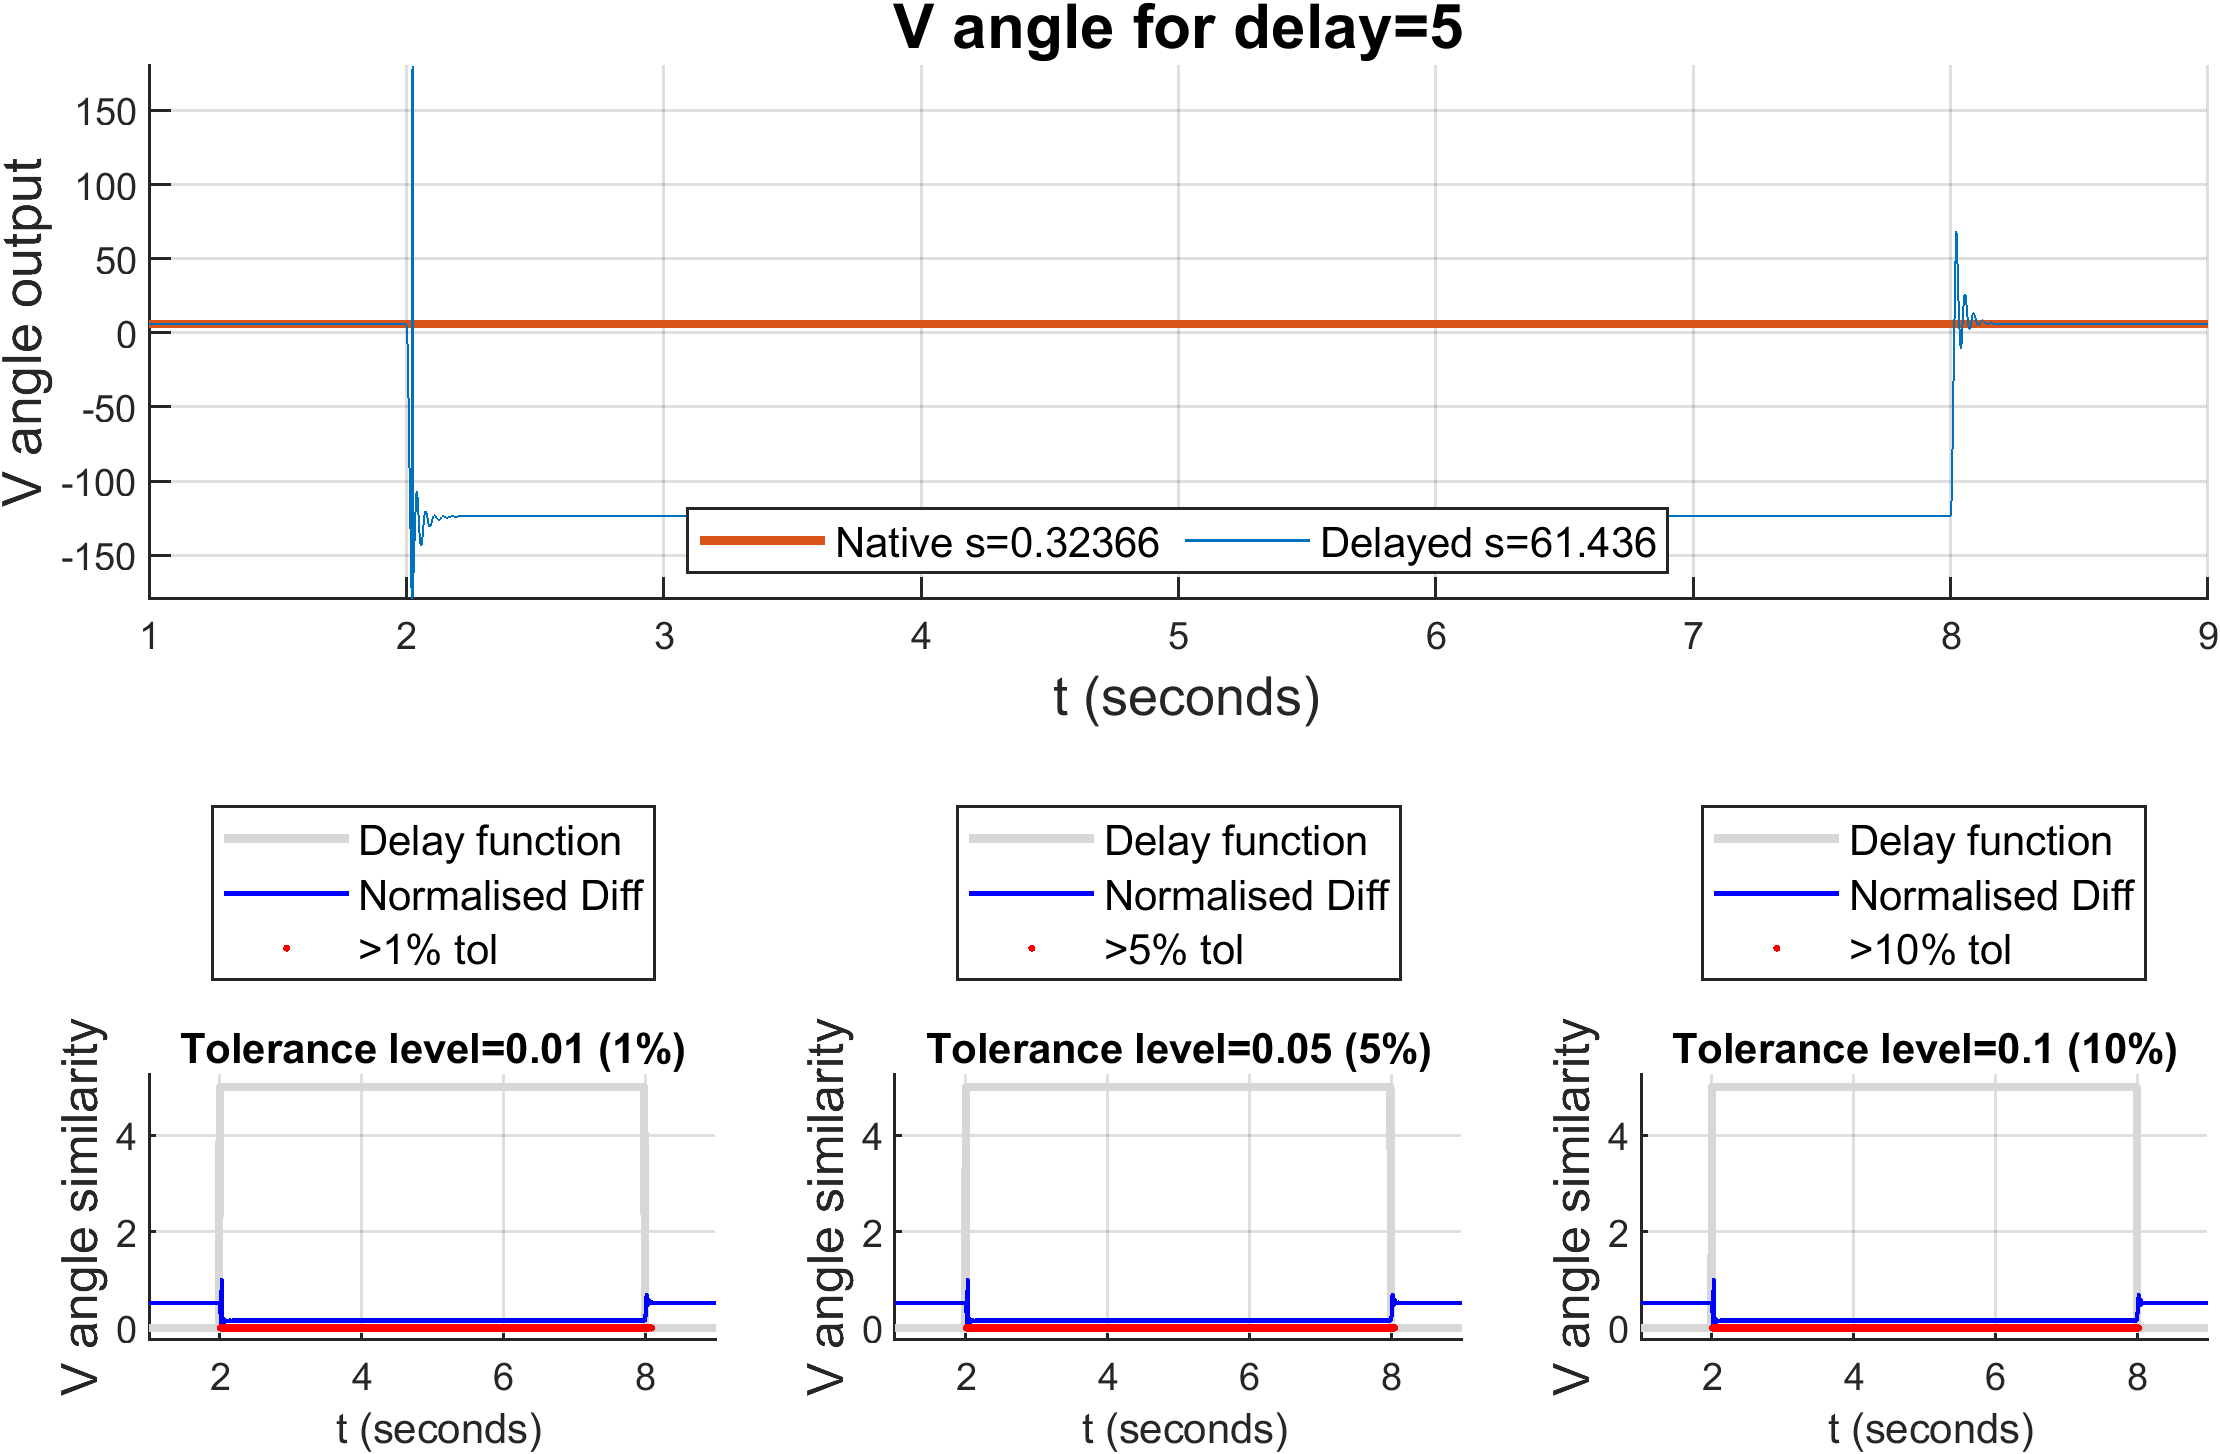
\includegraphics[width=0.95\textwidth]{PMUsim-figures/DelayOf_5/Instant_vAngle.png}    
    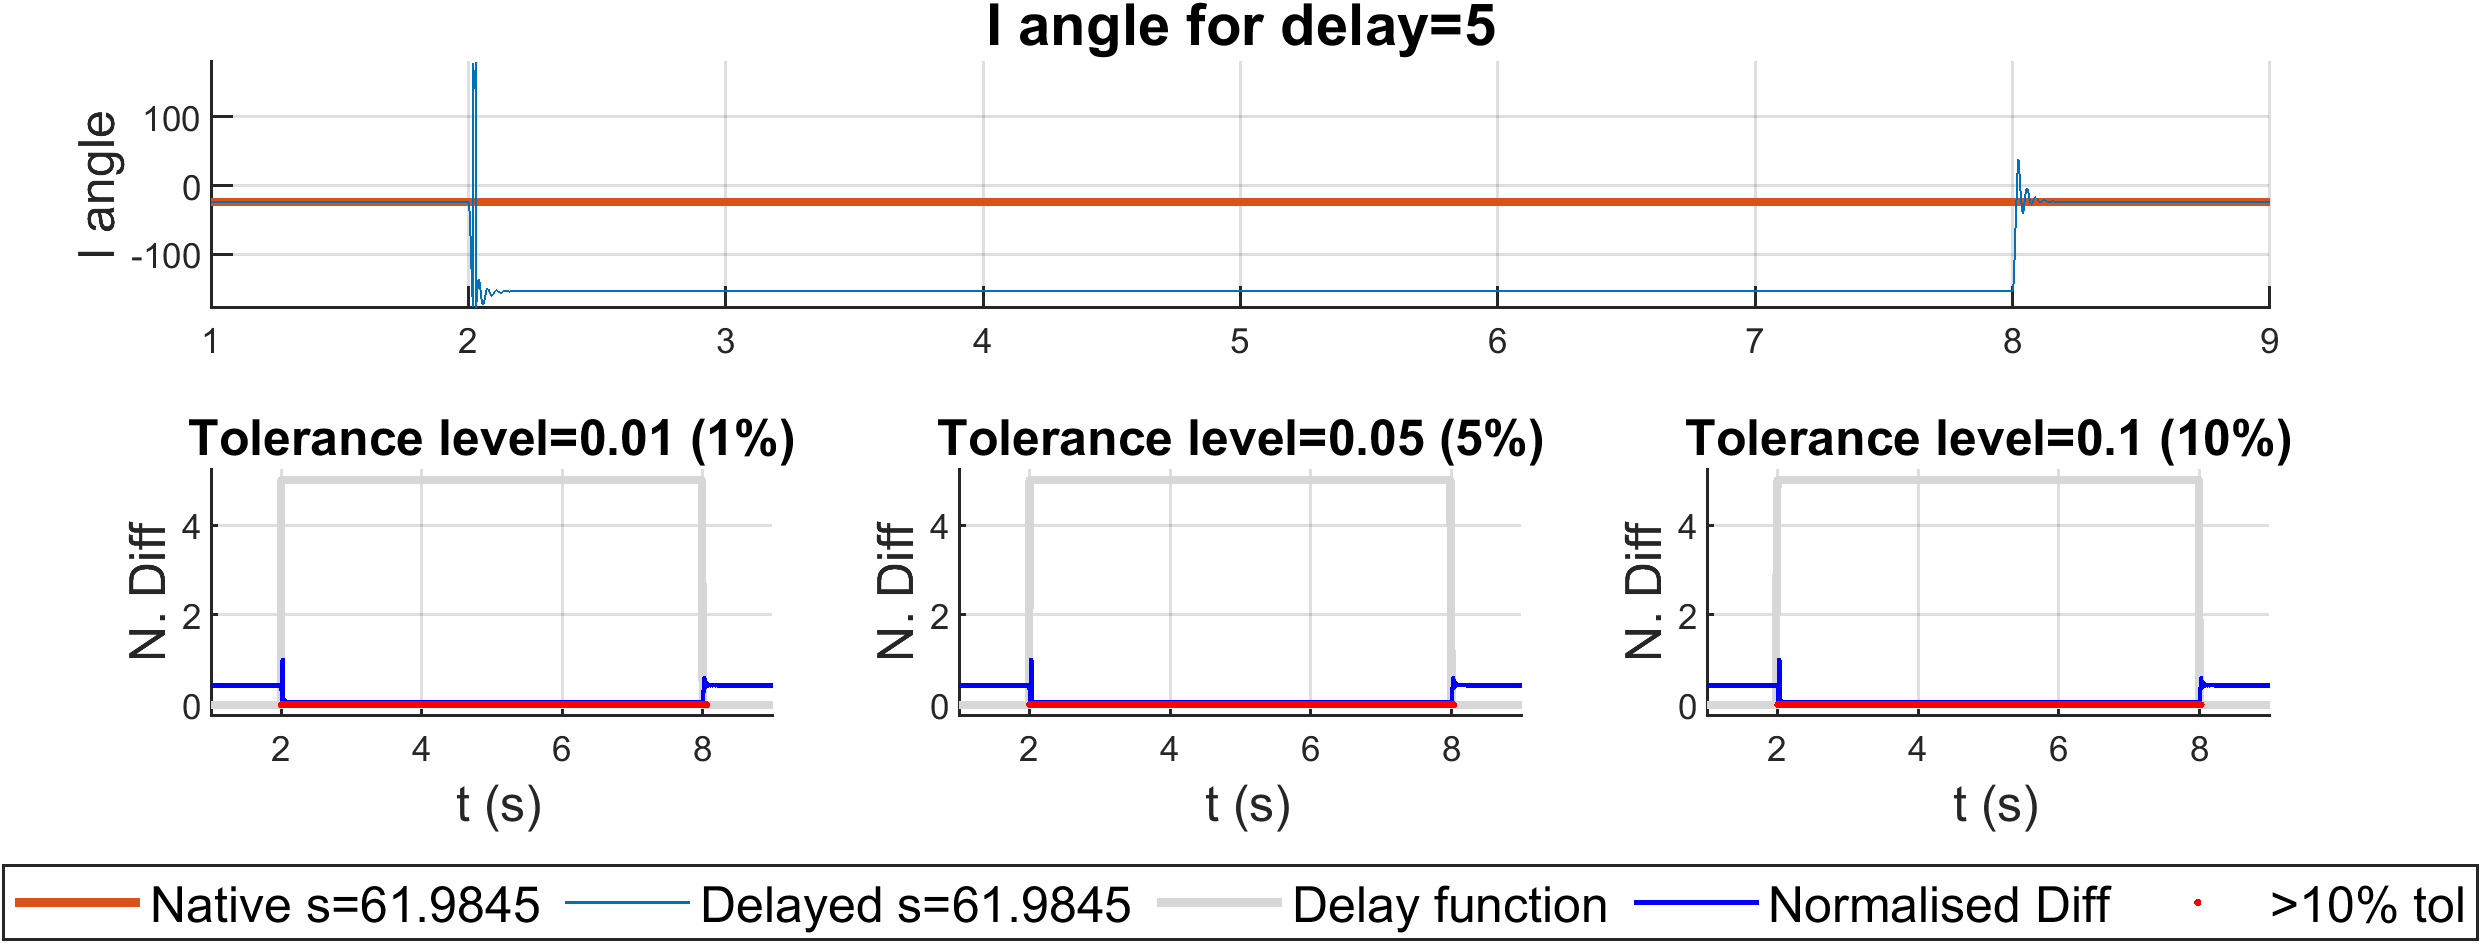
\includegraphics[width=0.95\textwidth]{PMUsim-figures/DelayOf_5/Instant_iAngle.png}    
    \label{fig:PMUsim_Five_Angle}
\end{floatingfigure}
        \begin{small}
     \tcbox[size=small, standard jigsaw, opacityback=0, boxrule=0pt,halign=justify]{
     Comment on the figure:}{
     \begin{itemize}
         \item 
     \end{itemize} }
     \end{small}

\newpage \subsection{Delay Level of Six}
\textbf{Results for Magnitude Output}

\begin{floatingfigure}[p]{\textwidth}
    \caption{Instant Delay Magnitude Output for the Delay Level of Six}
    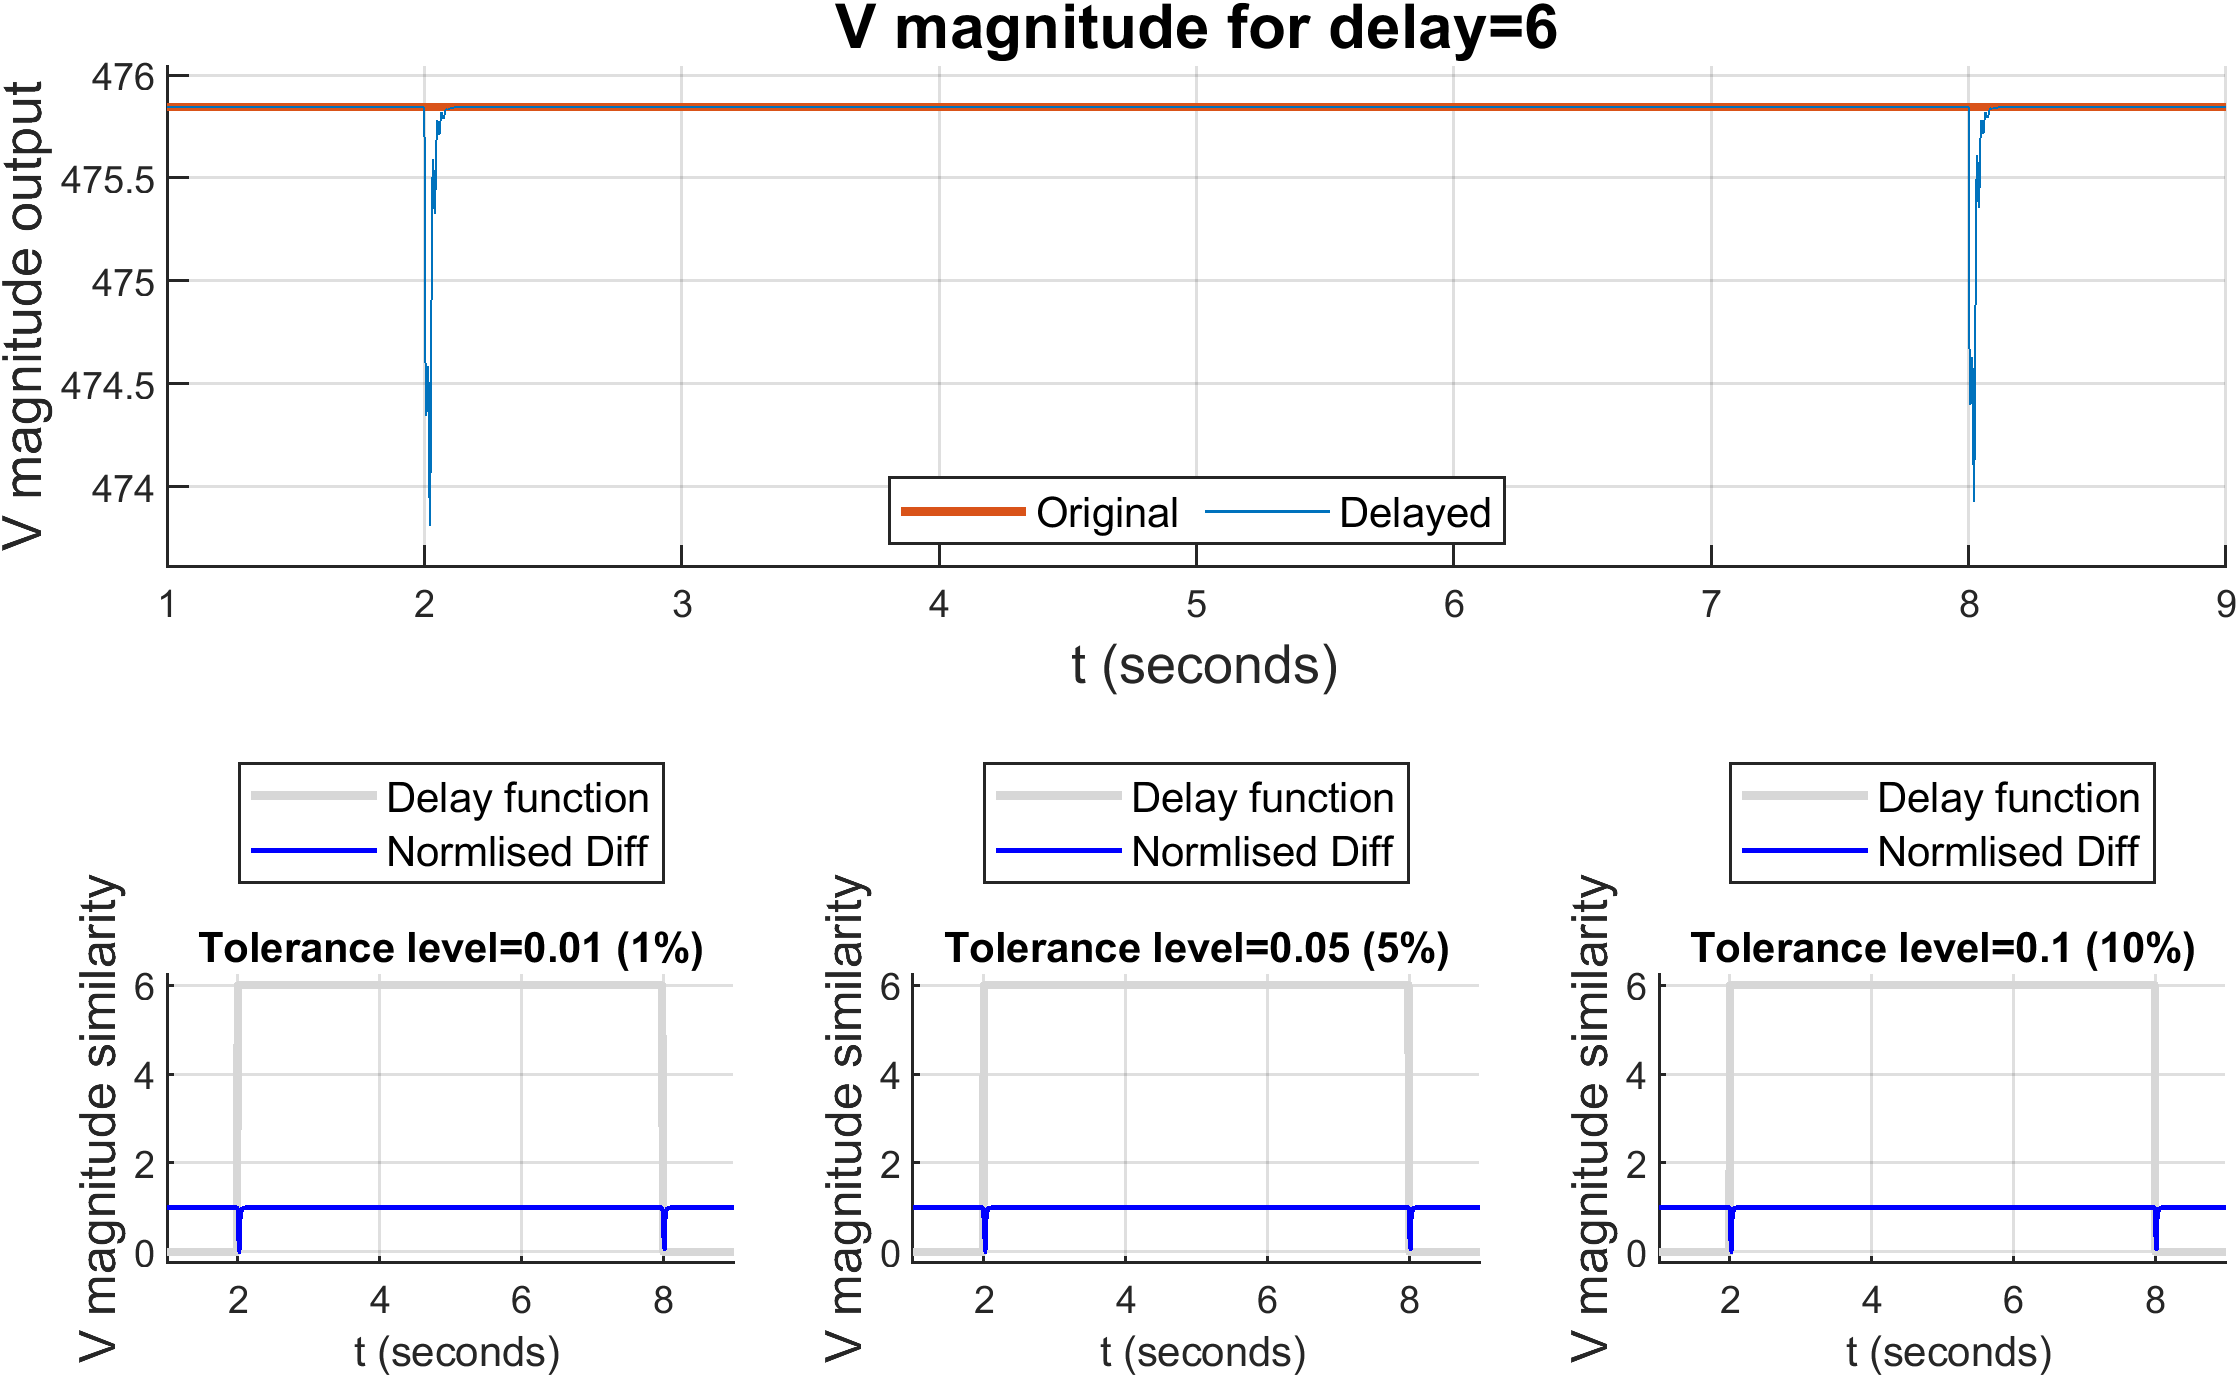
\includegraphics[width=0.95\textwidth]{PMUsim-figures/DelayOf_6/Instant_vMagnitude.png}    
      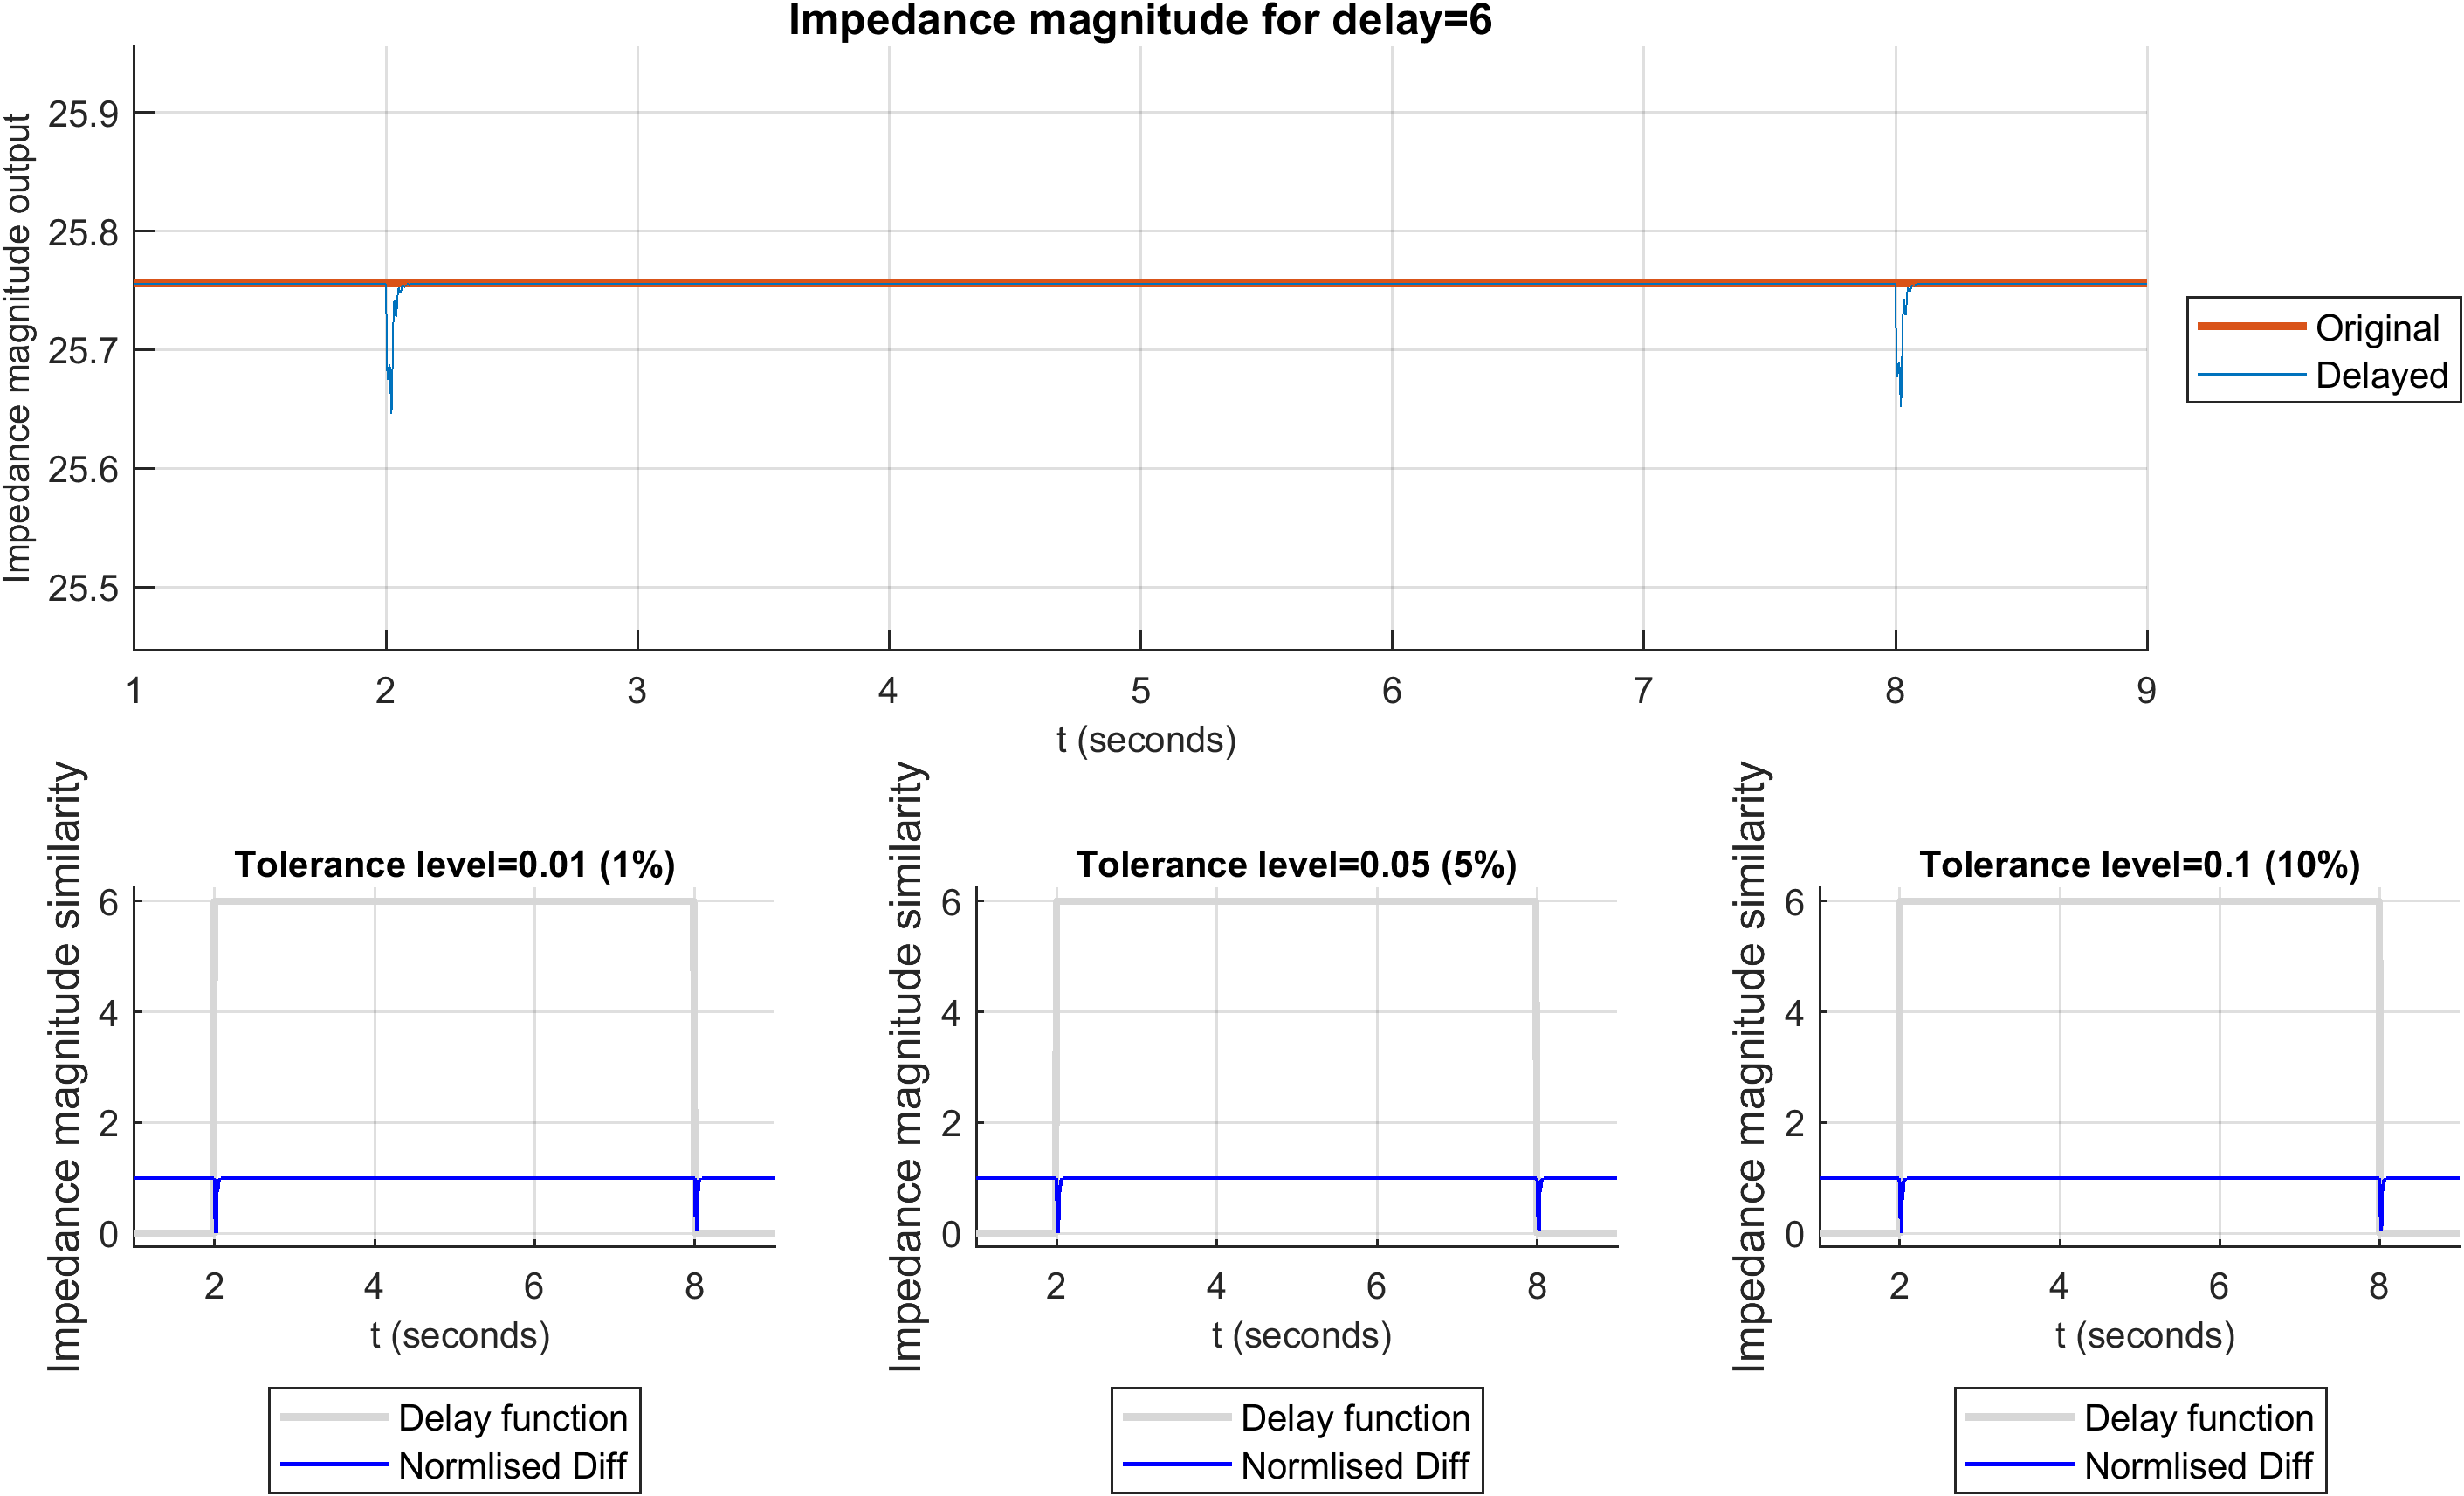
\includegraphics[width=0.95\textwidth]{PMUsim-figures/DelayOf_6/Instant_iMagnitude.png}       \label{fig:PMUsim_Six_Magnitude}
\end{floatingfigure}
    \begin{small}
     \tcbox[size=small, standard jigsaw, opacityback=0, boxrule=0pt,halign=justify]{
     Comment on the figure:}{
     \begin{itemize}
         \item 
     \end{itemize} }
     \end{small}

\newpage \textbf{Results for Frequency Output}


\begin{floatingfigure}[p]{\textwidth}
    \caption{Instant Delay Frequency Output for the Delay Level of Six}
    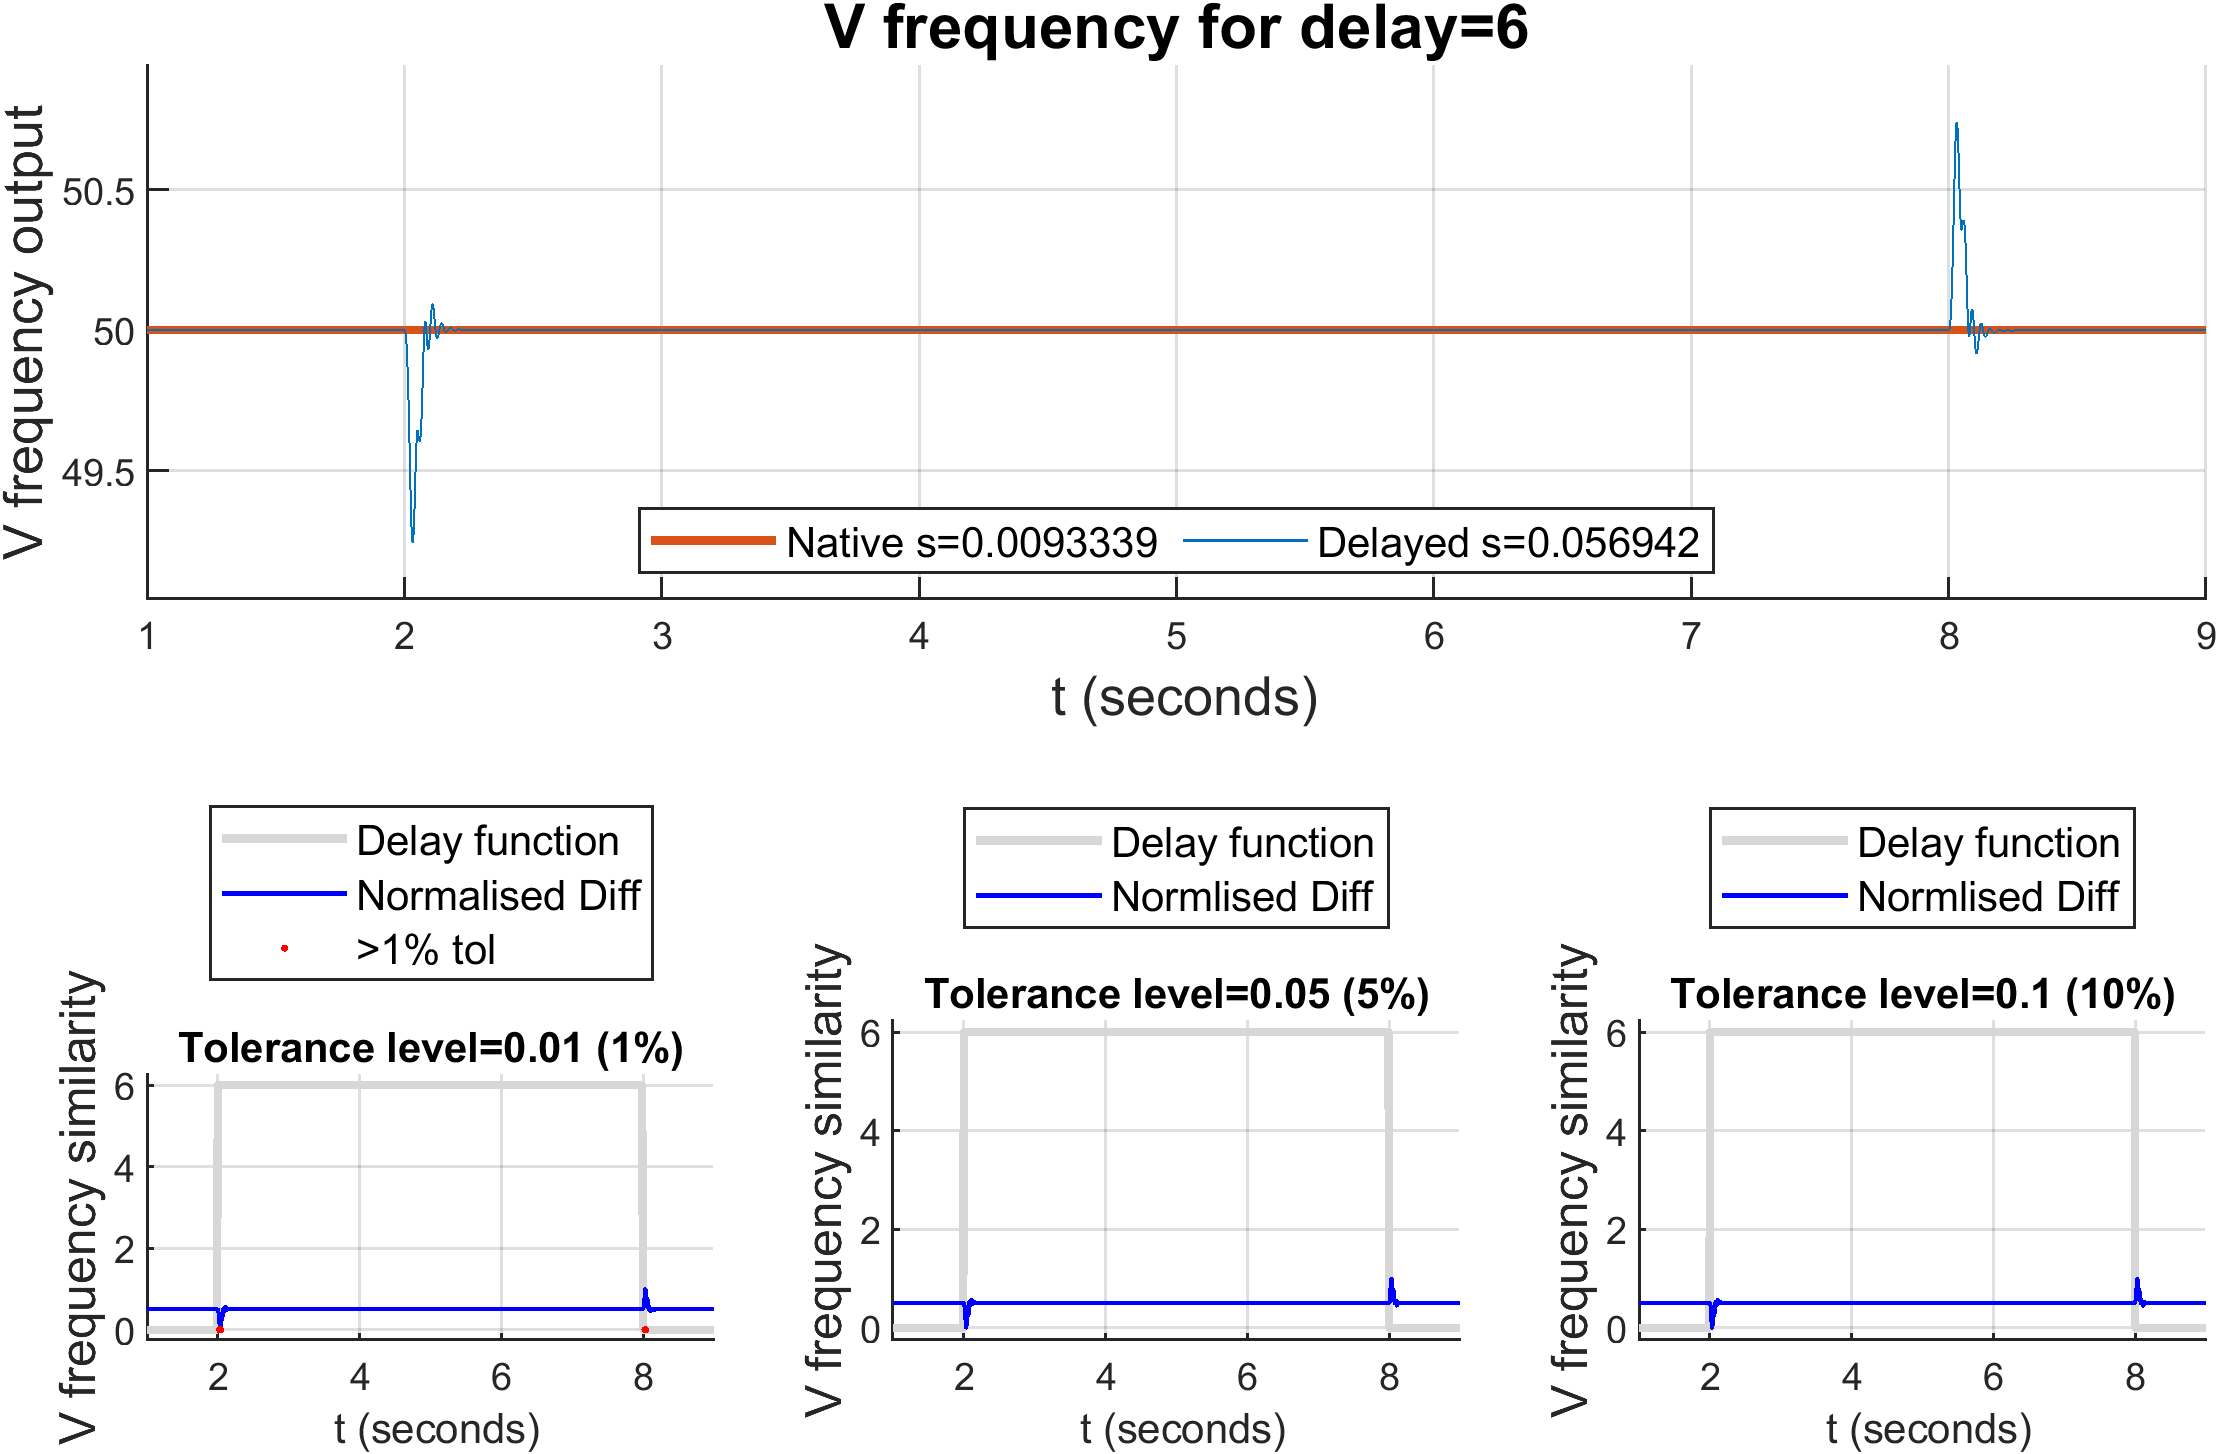
\includegraphics[width=0.95\textwidth]{PMUsim-figures/DelayOf_6/Instant_vFrequency.png}    
    \label{fig:PMUsim_Six_vFrequency}
    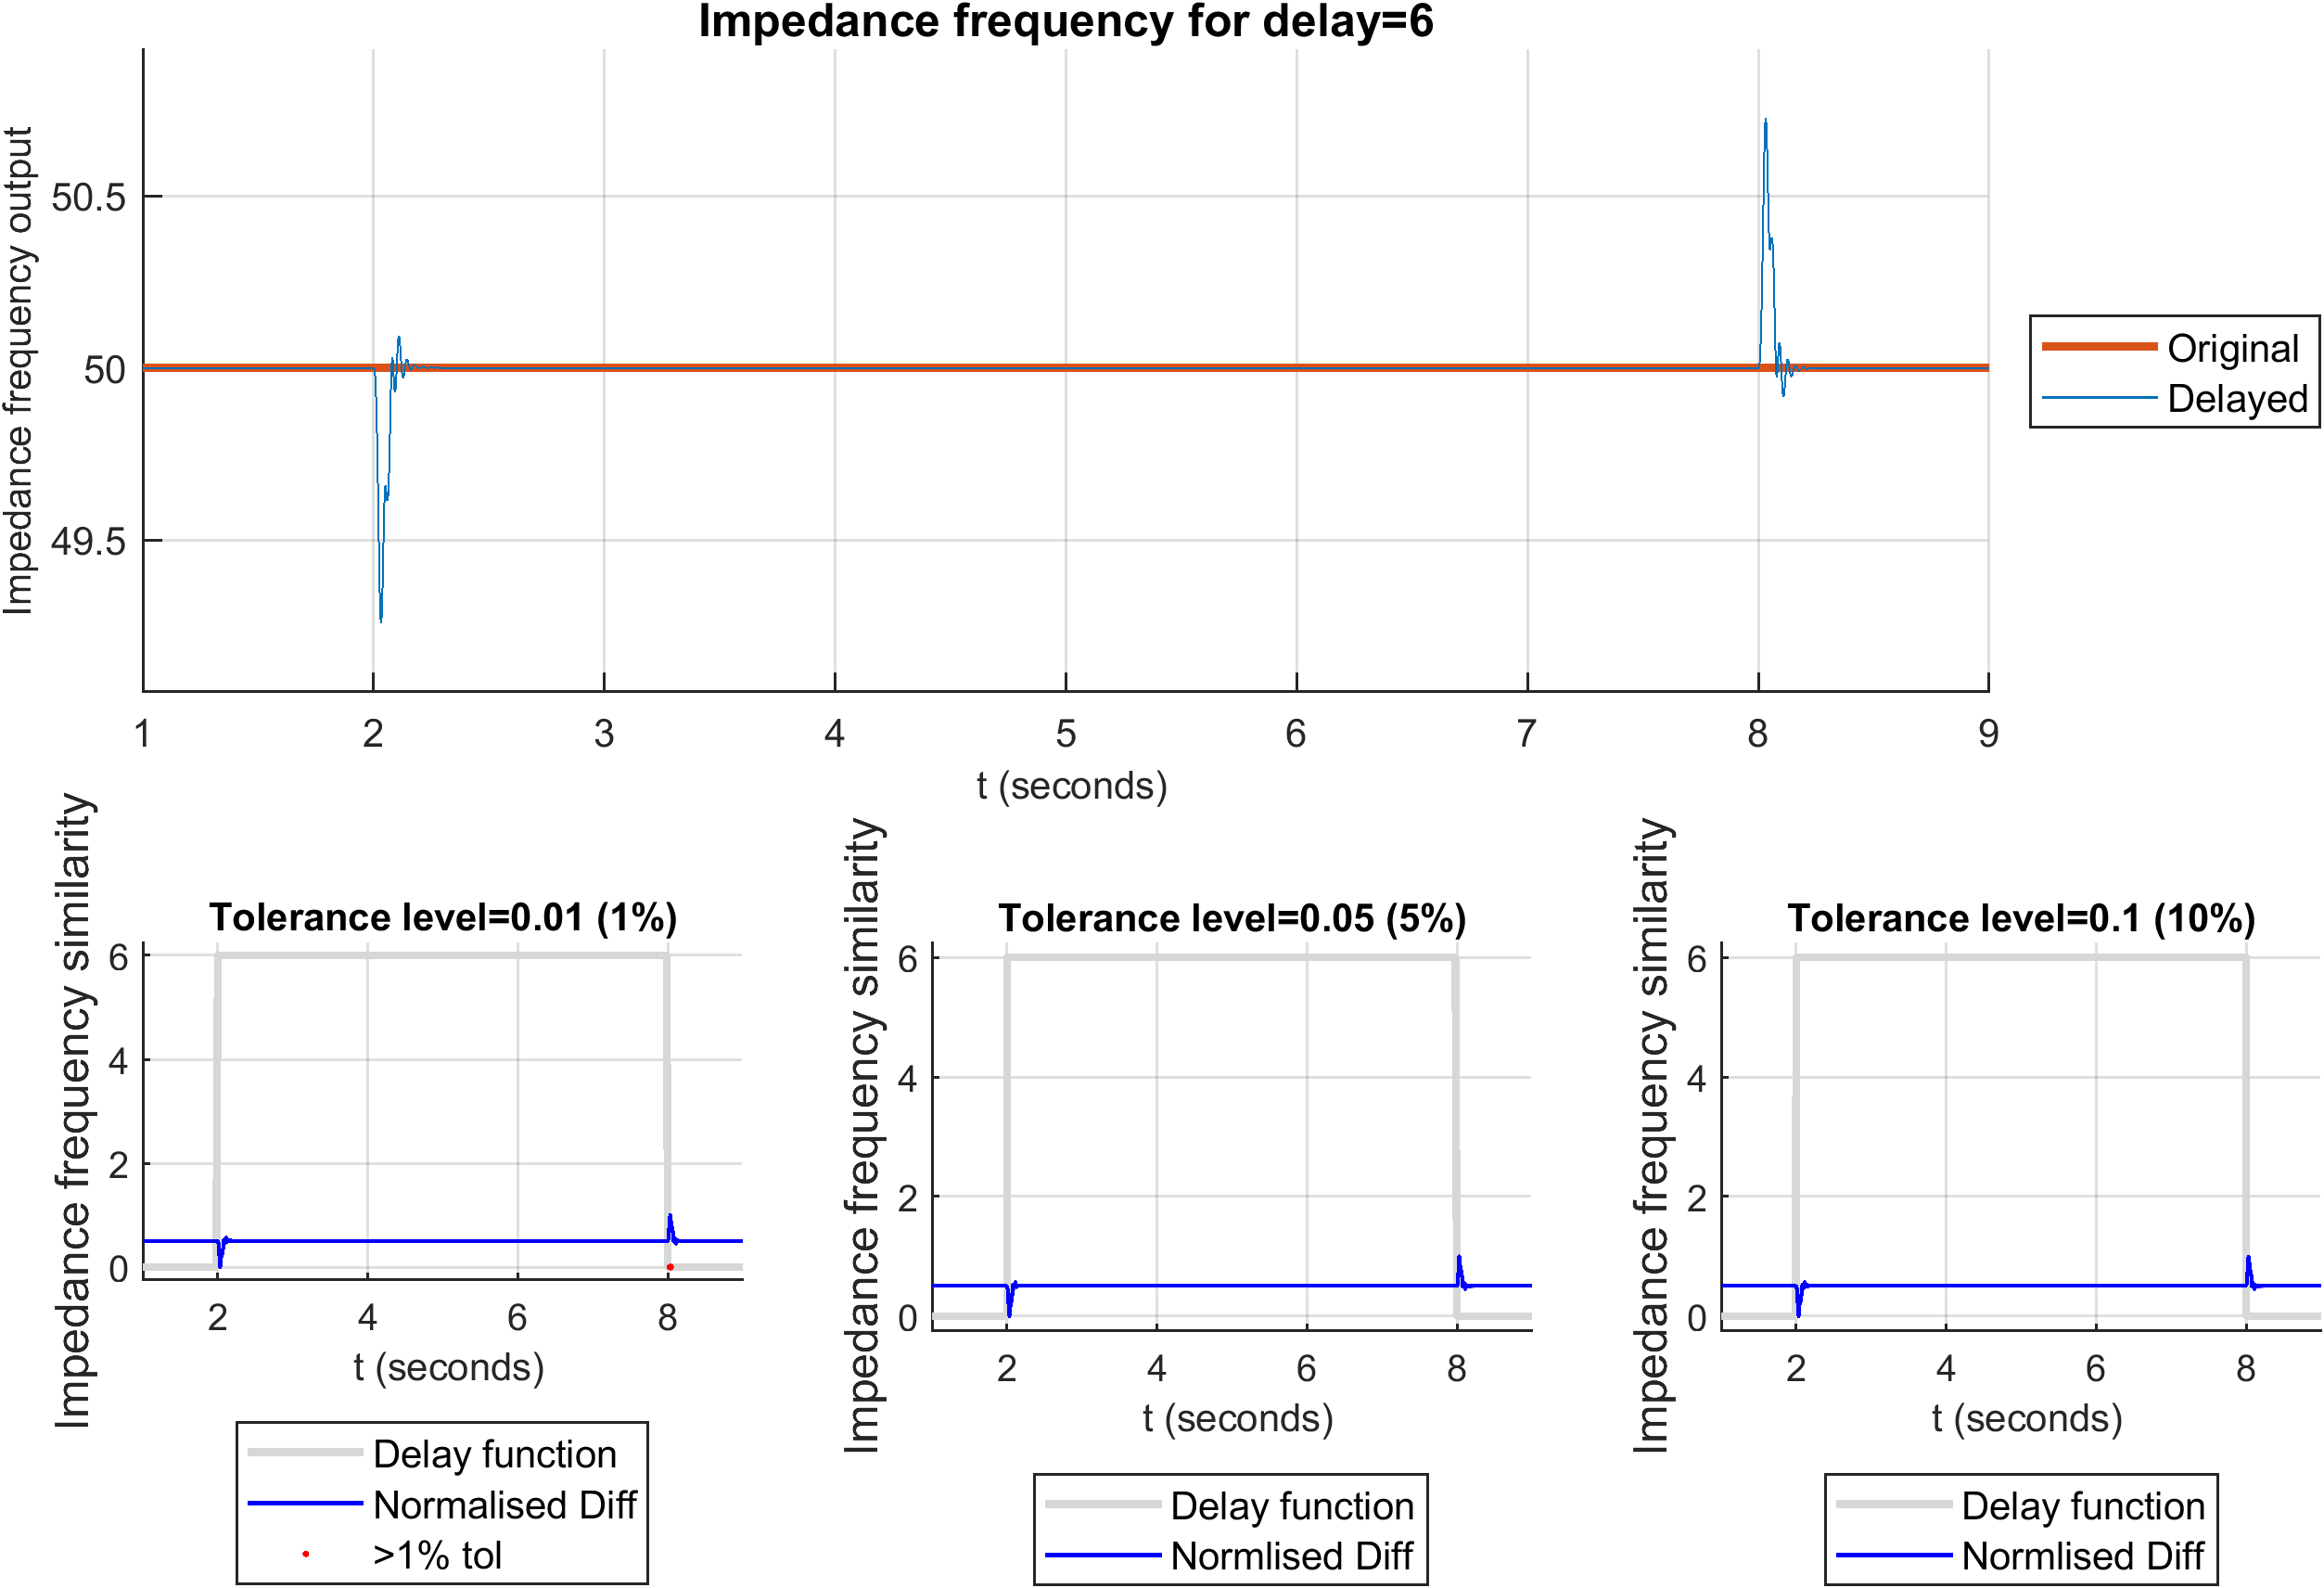
\includegraphics[width=0.95\textwidth]{PMUsim-figures/DelayOf_6/Instant_iFrequency.png}    
    \label{fig:PMUsim_Six_Frequency}
\end{floatingfigure}
        \begin{small}
     \tcbox[size=small, standard jigsaw, opacityback=0, boxrule=0pt,halign=justify]{
     Comment on the figure:}{
     \begin{itemize}
         \item 
     \end{itemize} }
     \end{small}


\newpage \textbf{Results for Angle Output}


\begin{floatingfigure}[p]{\textwidth}
    \caption{Instant Delay Angle Output for the Delay Level of Six}
    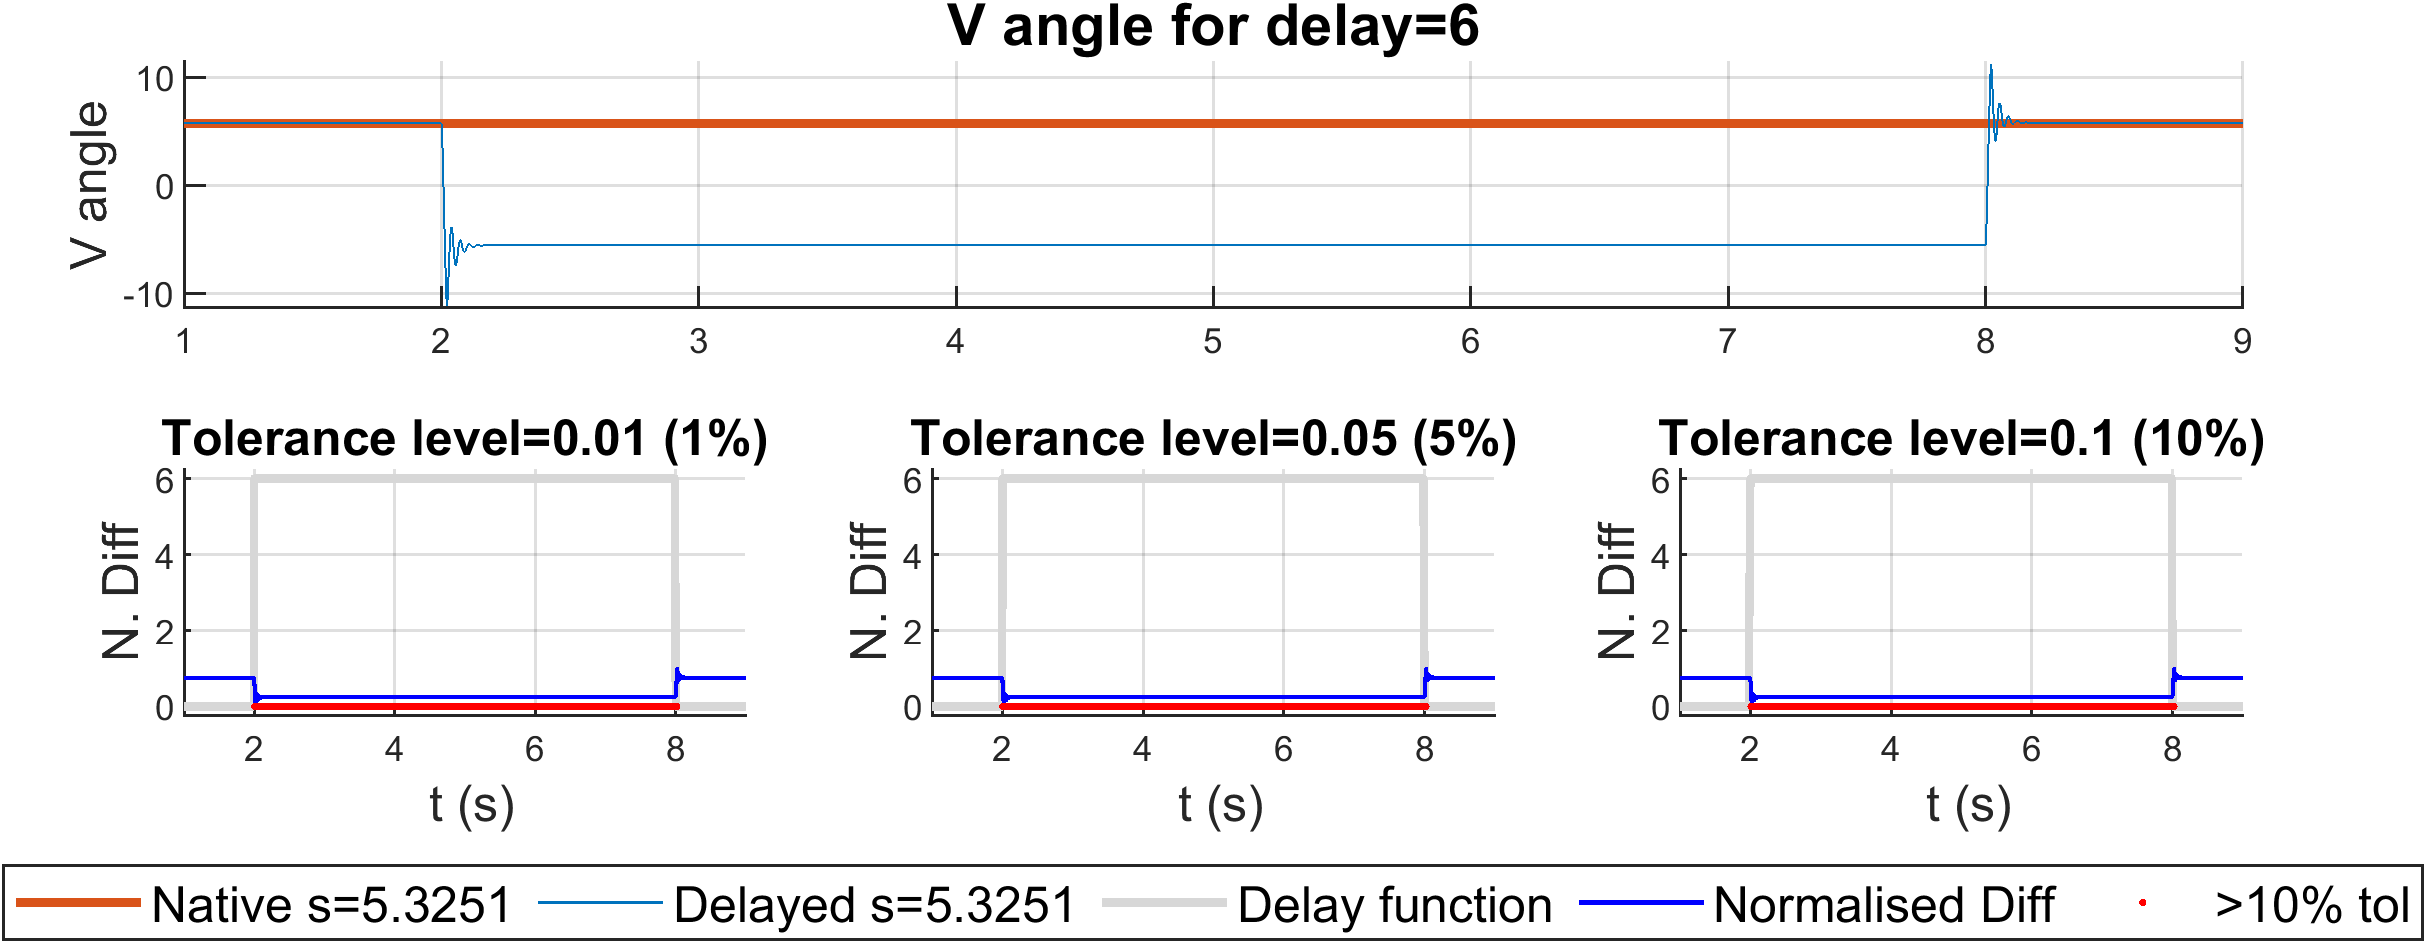
\includegraphics[width=0.95\textwidth]{PMUsim-figures/DelayOf_6/Instant_vAngle.png}    
    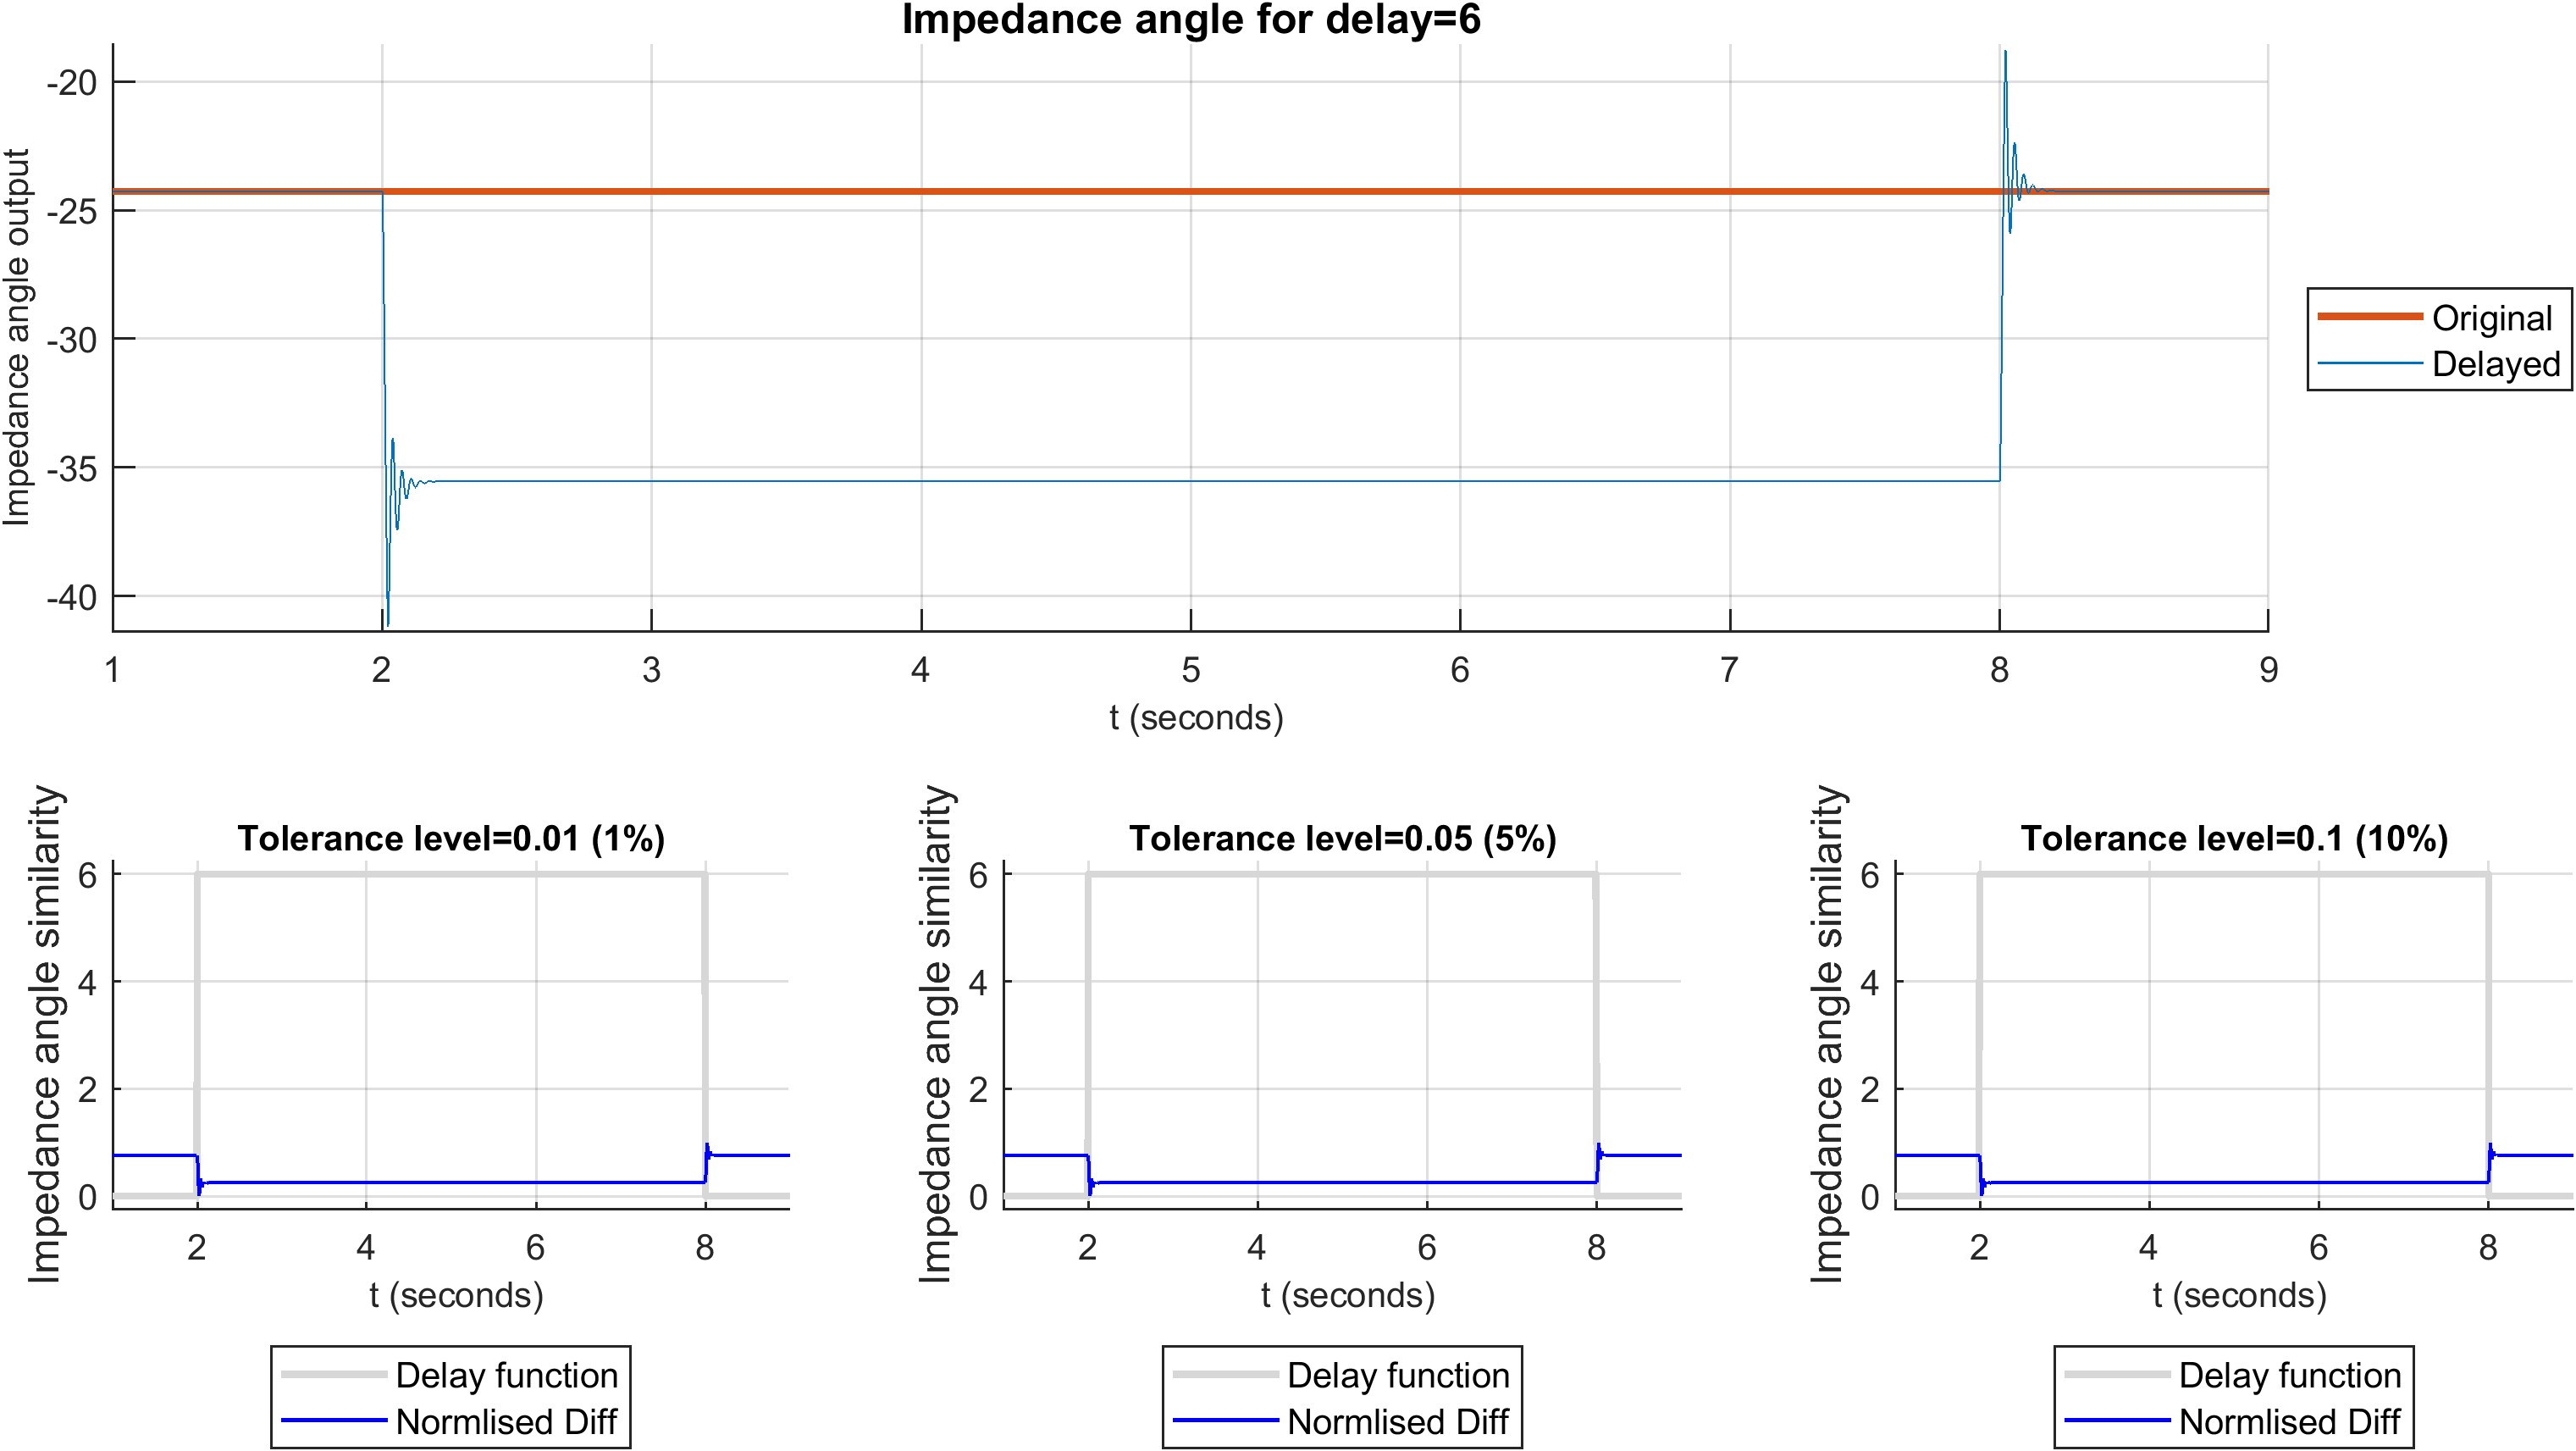
\includegraphics[width=0.95\textwidth]{PMUsim-figures/DelayOf_6/Instant_iAngle.png}    
    \label{fig:PMUsim_Six_Angle}
\end{floatingfigure}
        \begin{small}
     \tcbox[size=small, standard jigsaw, opacityback=0, boxrule=0pt,halign=justify]{
     Comment on the figure:}{
     \begin{itemize}
         \item 
     \end{itemize} }
     \end{small}


\section{Step-Wise Delay Functions}
\newpage \subsection{Delay Level of Two}
\textbf{Results for Magnitude Output}

\begin{floatingfigure}[p]{\textwidth}
    \caption{Step-Wise Delay Magnitude Output for the Delay Level of Two}
    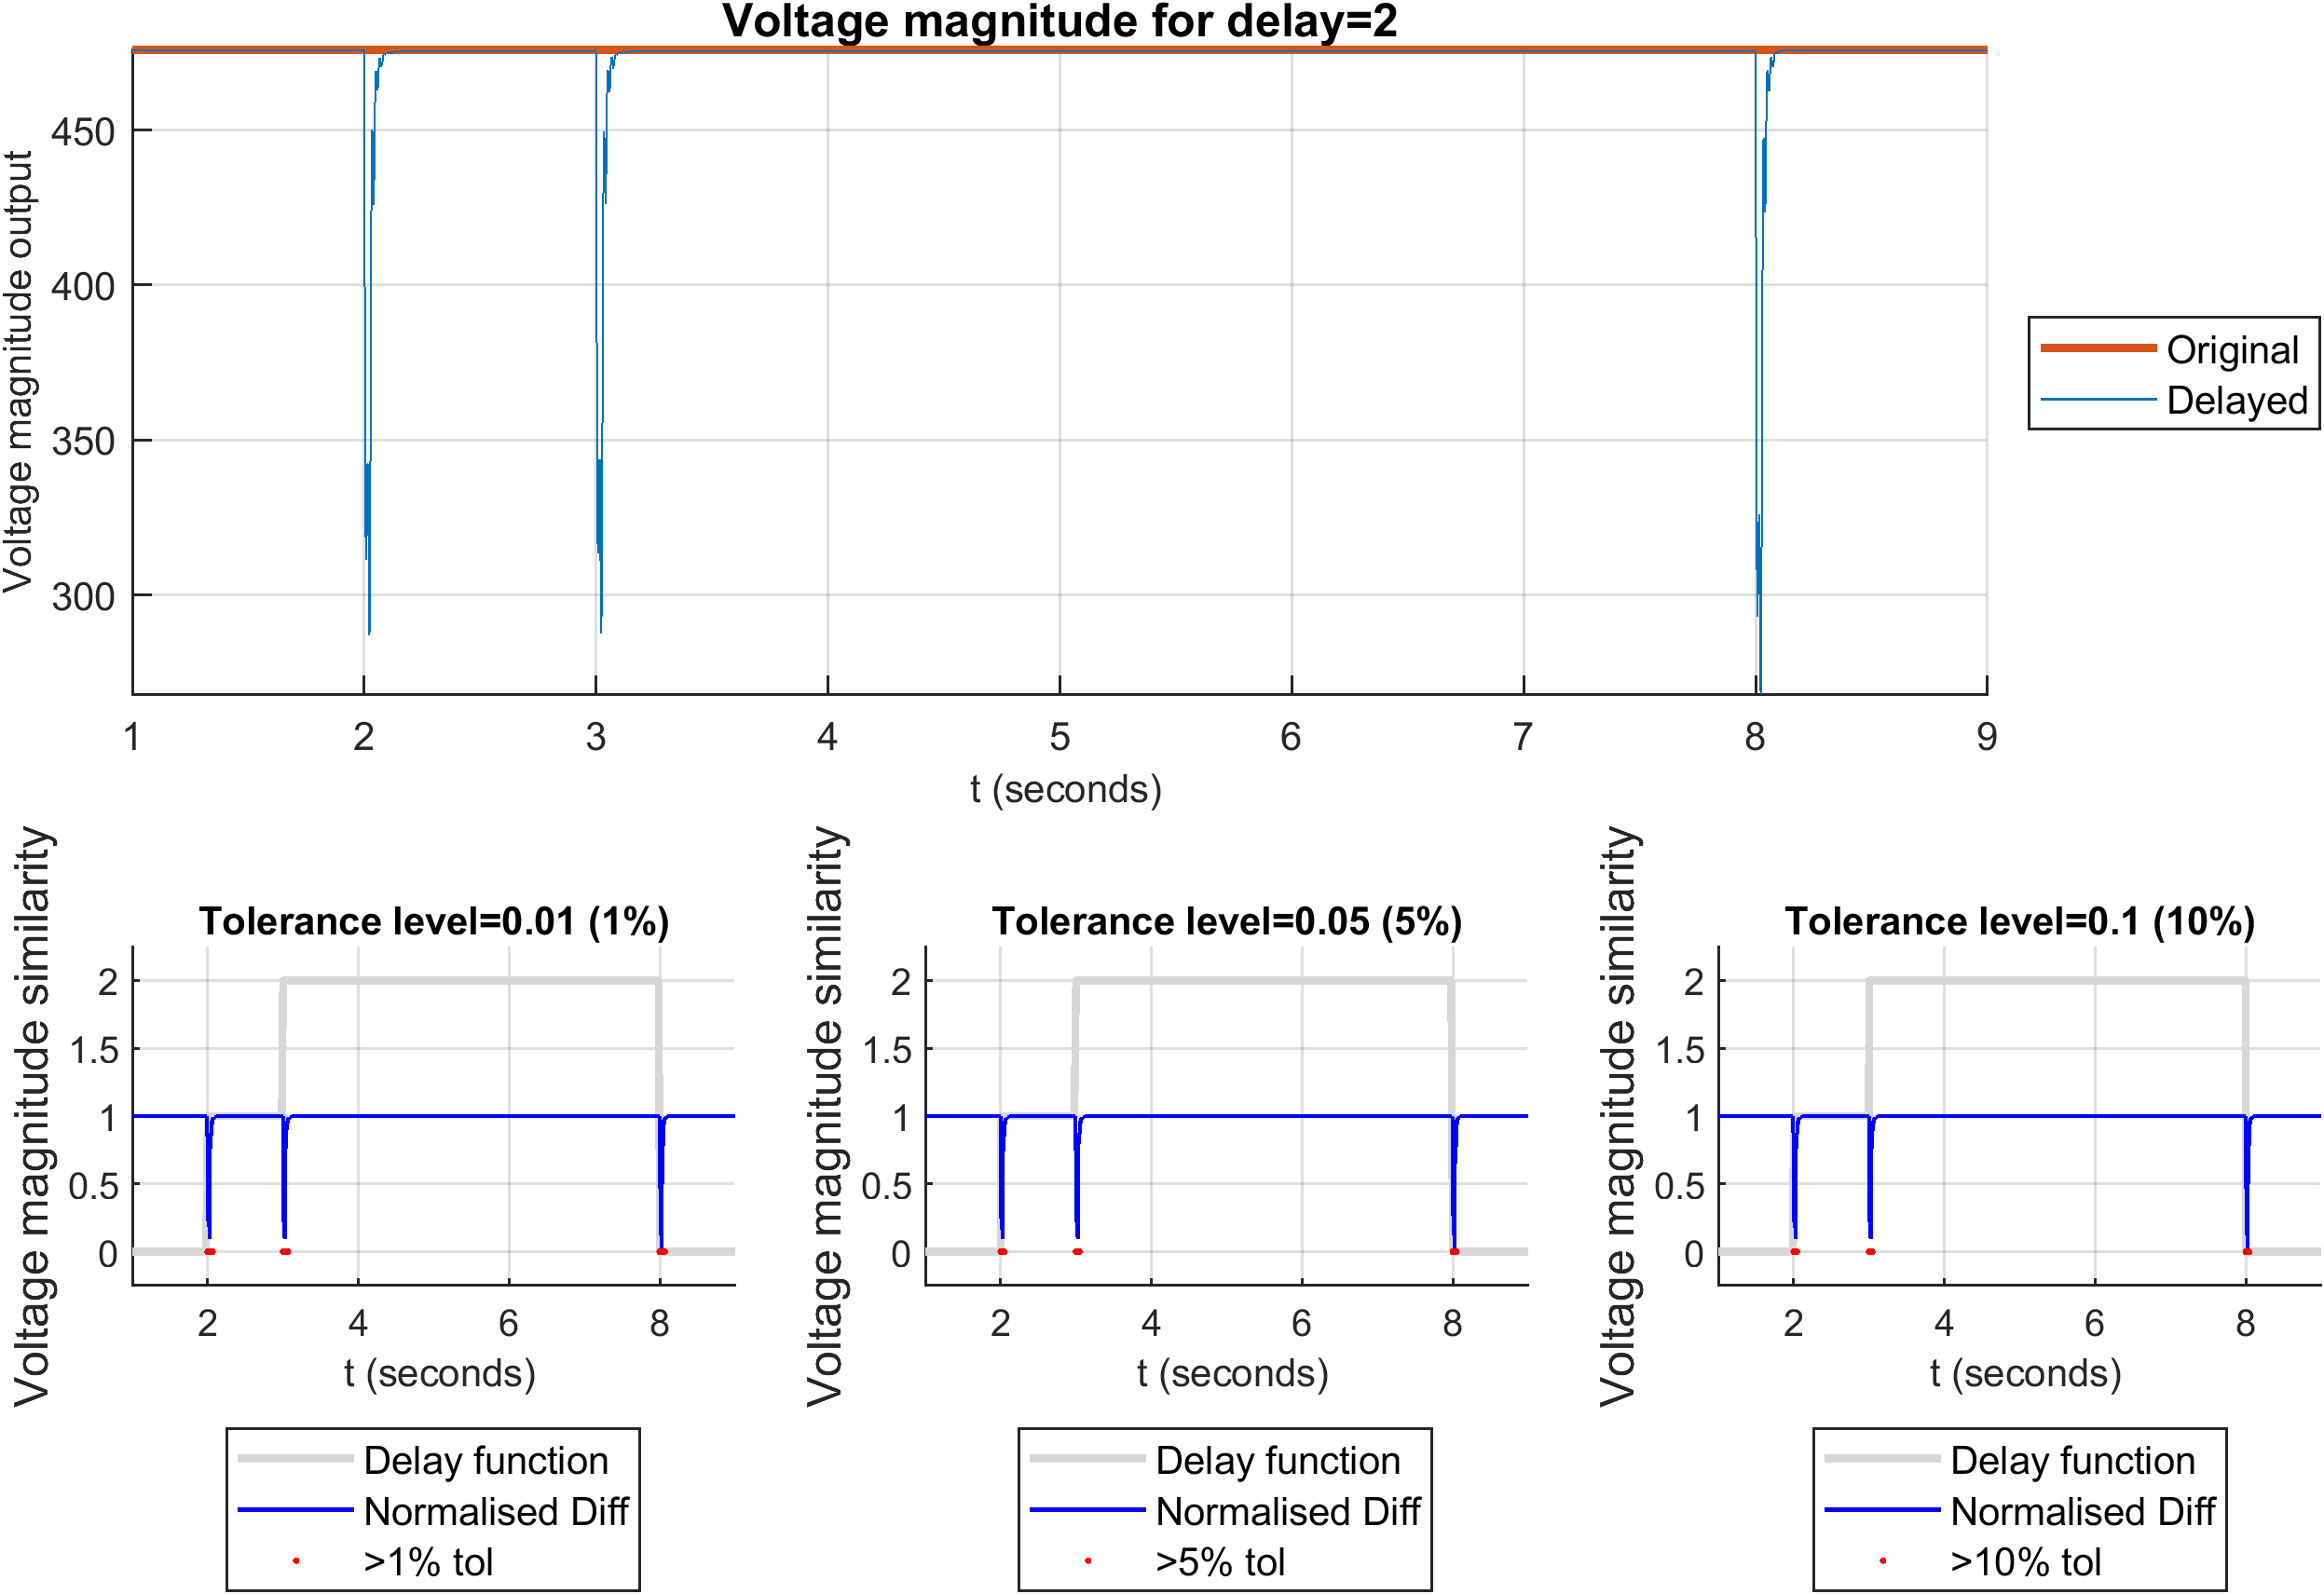
\includegraphics[width=0.95\textwidth]{PMUsim-figures/DelayOf_2/Step_vMagnitude.png}    
      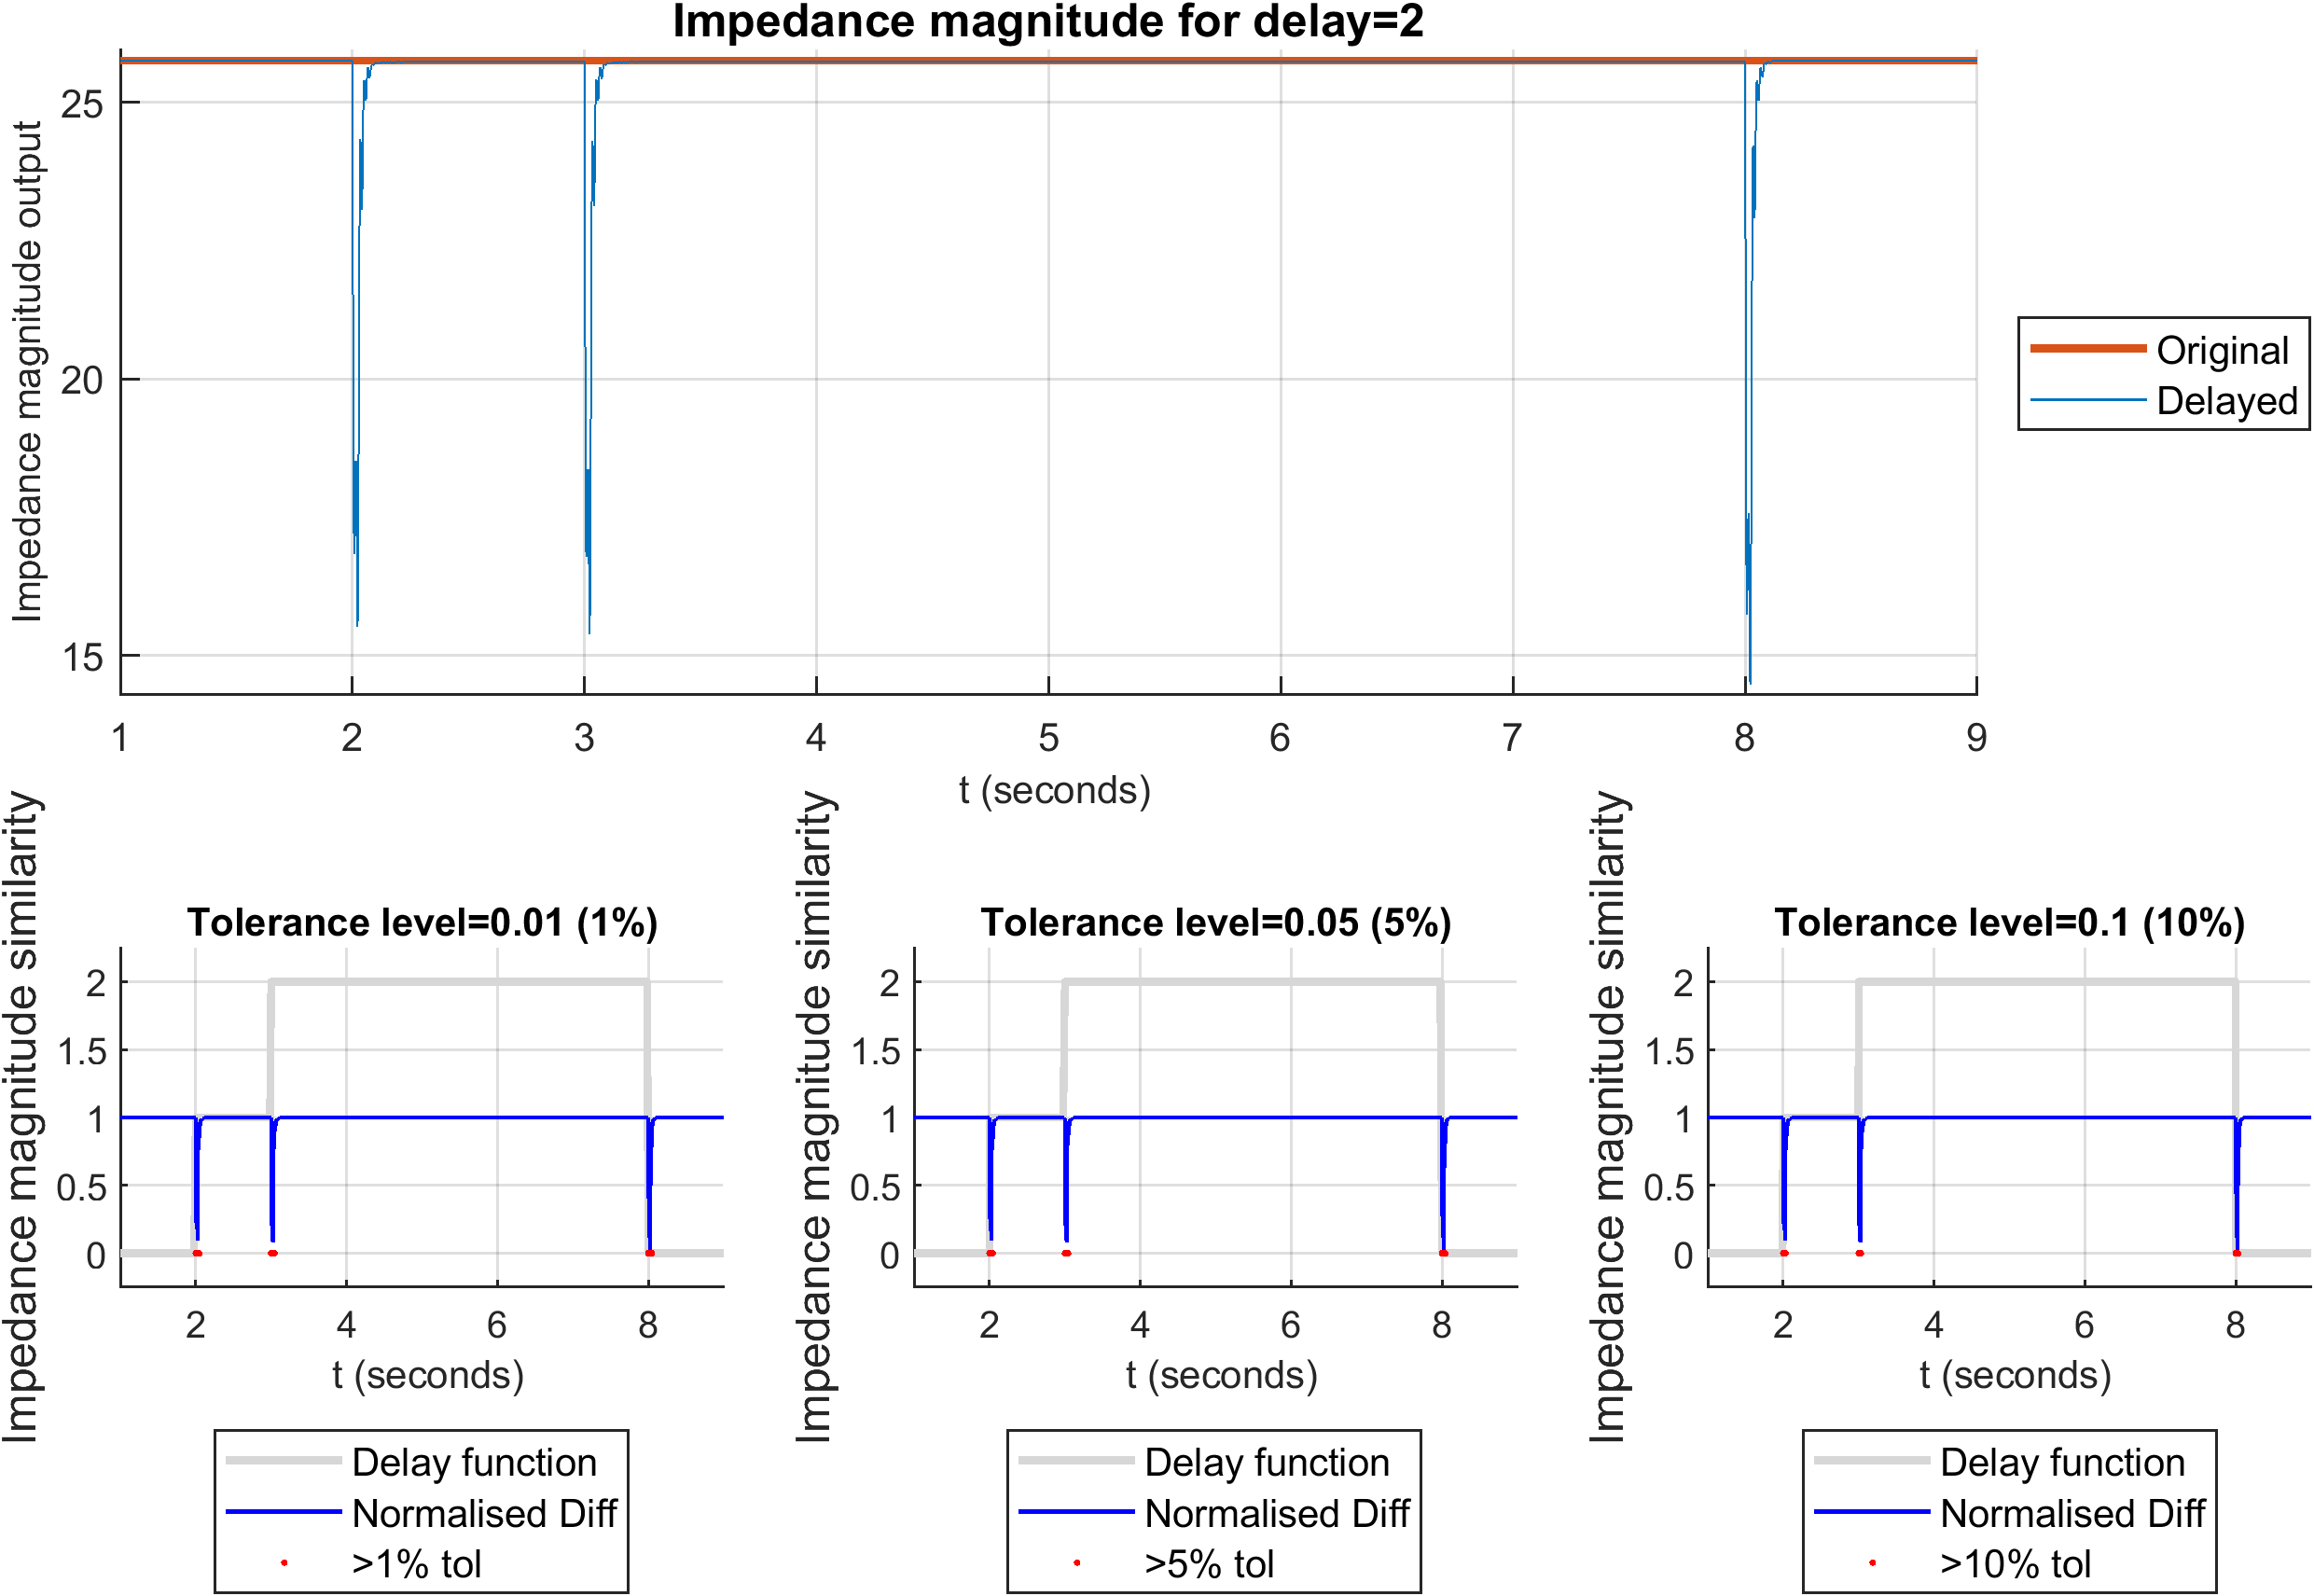
\includegraphics[width=0.95\textwidth]{PMUsim-figures/DelayOf_2/Step_iMagnitude.png}    
    \label{fig:PMUsimStep_Two_Magnitude}
\end{floatingfigure}
    \begin{small}
     \tcbox[size=small, standard jigsaw, opacityback=0, boxrule=0pt,halign=justify]{
     Comment on the figure:}{
          \begin{itemize}
         \item 
     \end{itemize} }
     \end{small}

\newpage \textbf{Results for Frequency Output}


\begin{floatingfigure}[p]{\textwidth}
    \caption{Step-Wise Delay Frequency Output for the Delay Level of Two}
    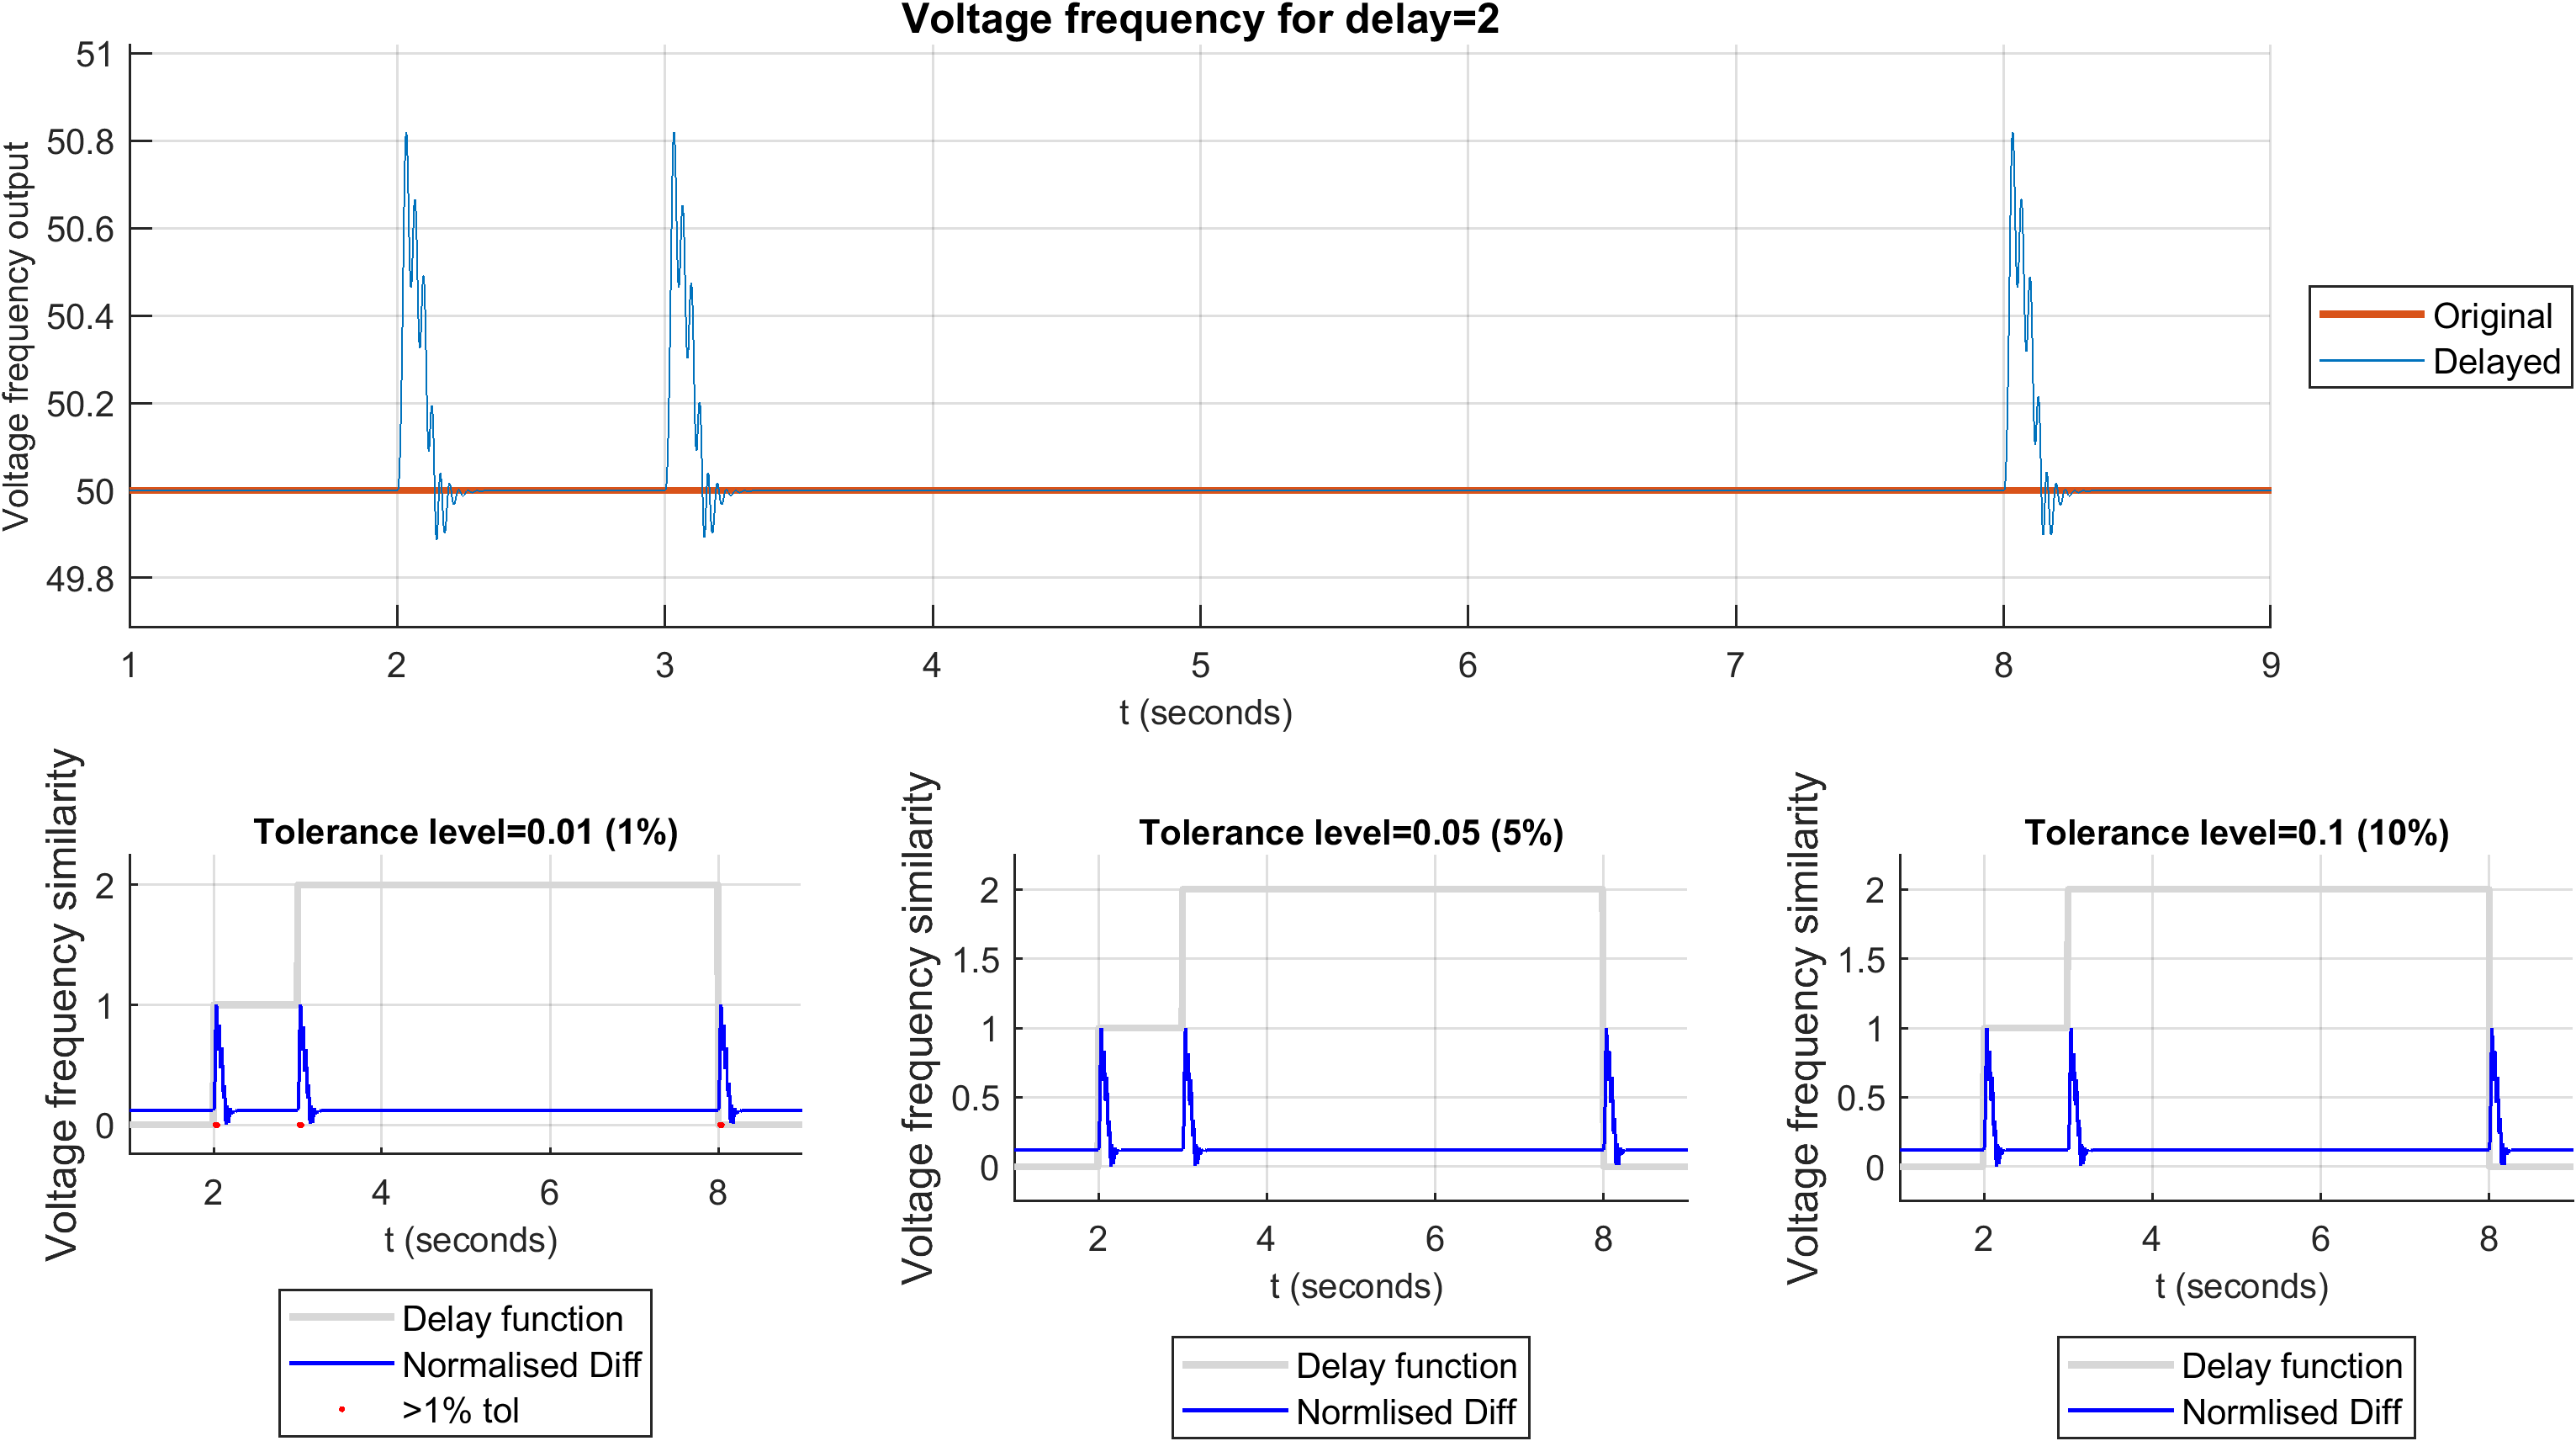
\includegraphics[width=0.95\textwidth]{PMUsim-figures/DelayOf_2/Step_vFrequency.png}    
    \label{fig:PMUsimStep_Two_vFrequency}
    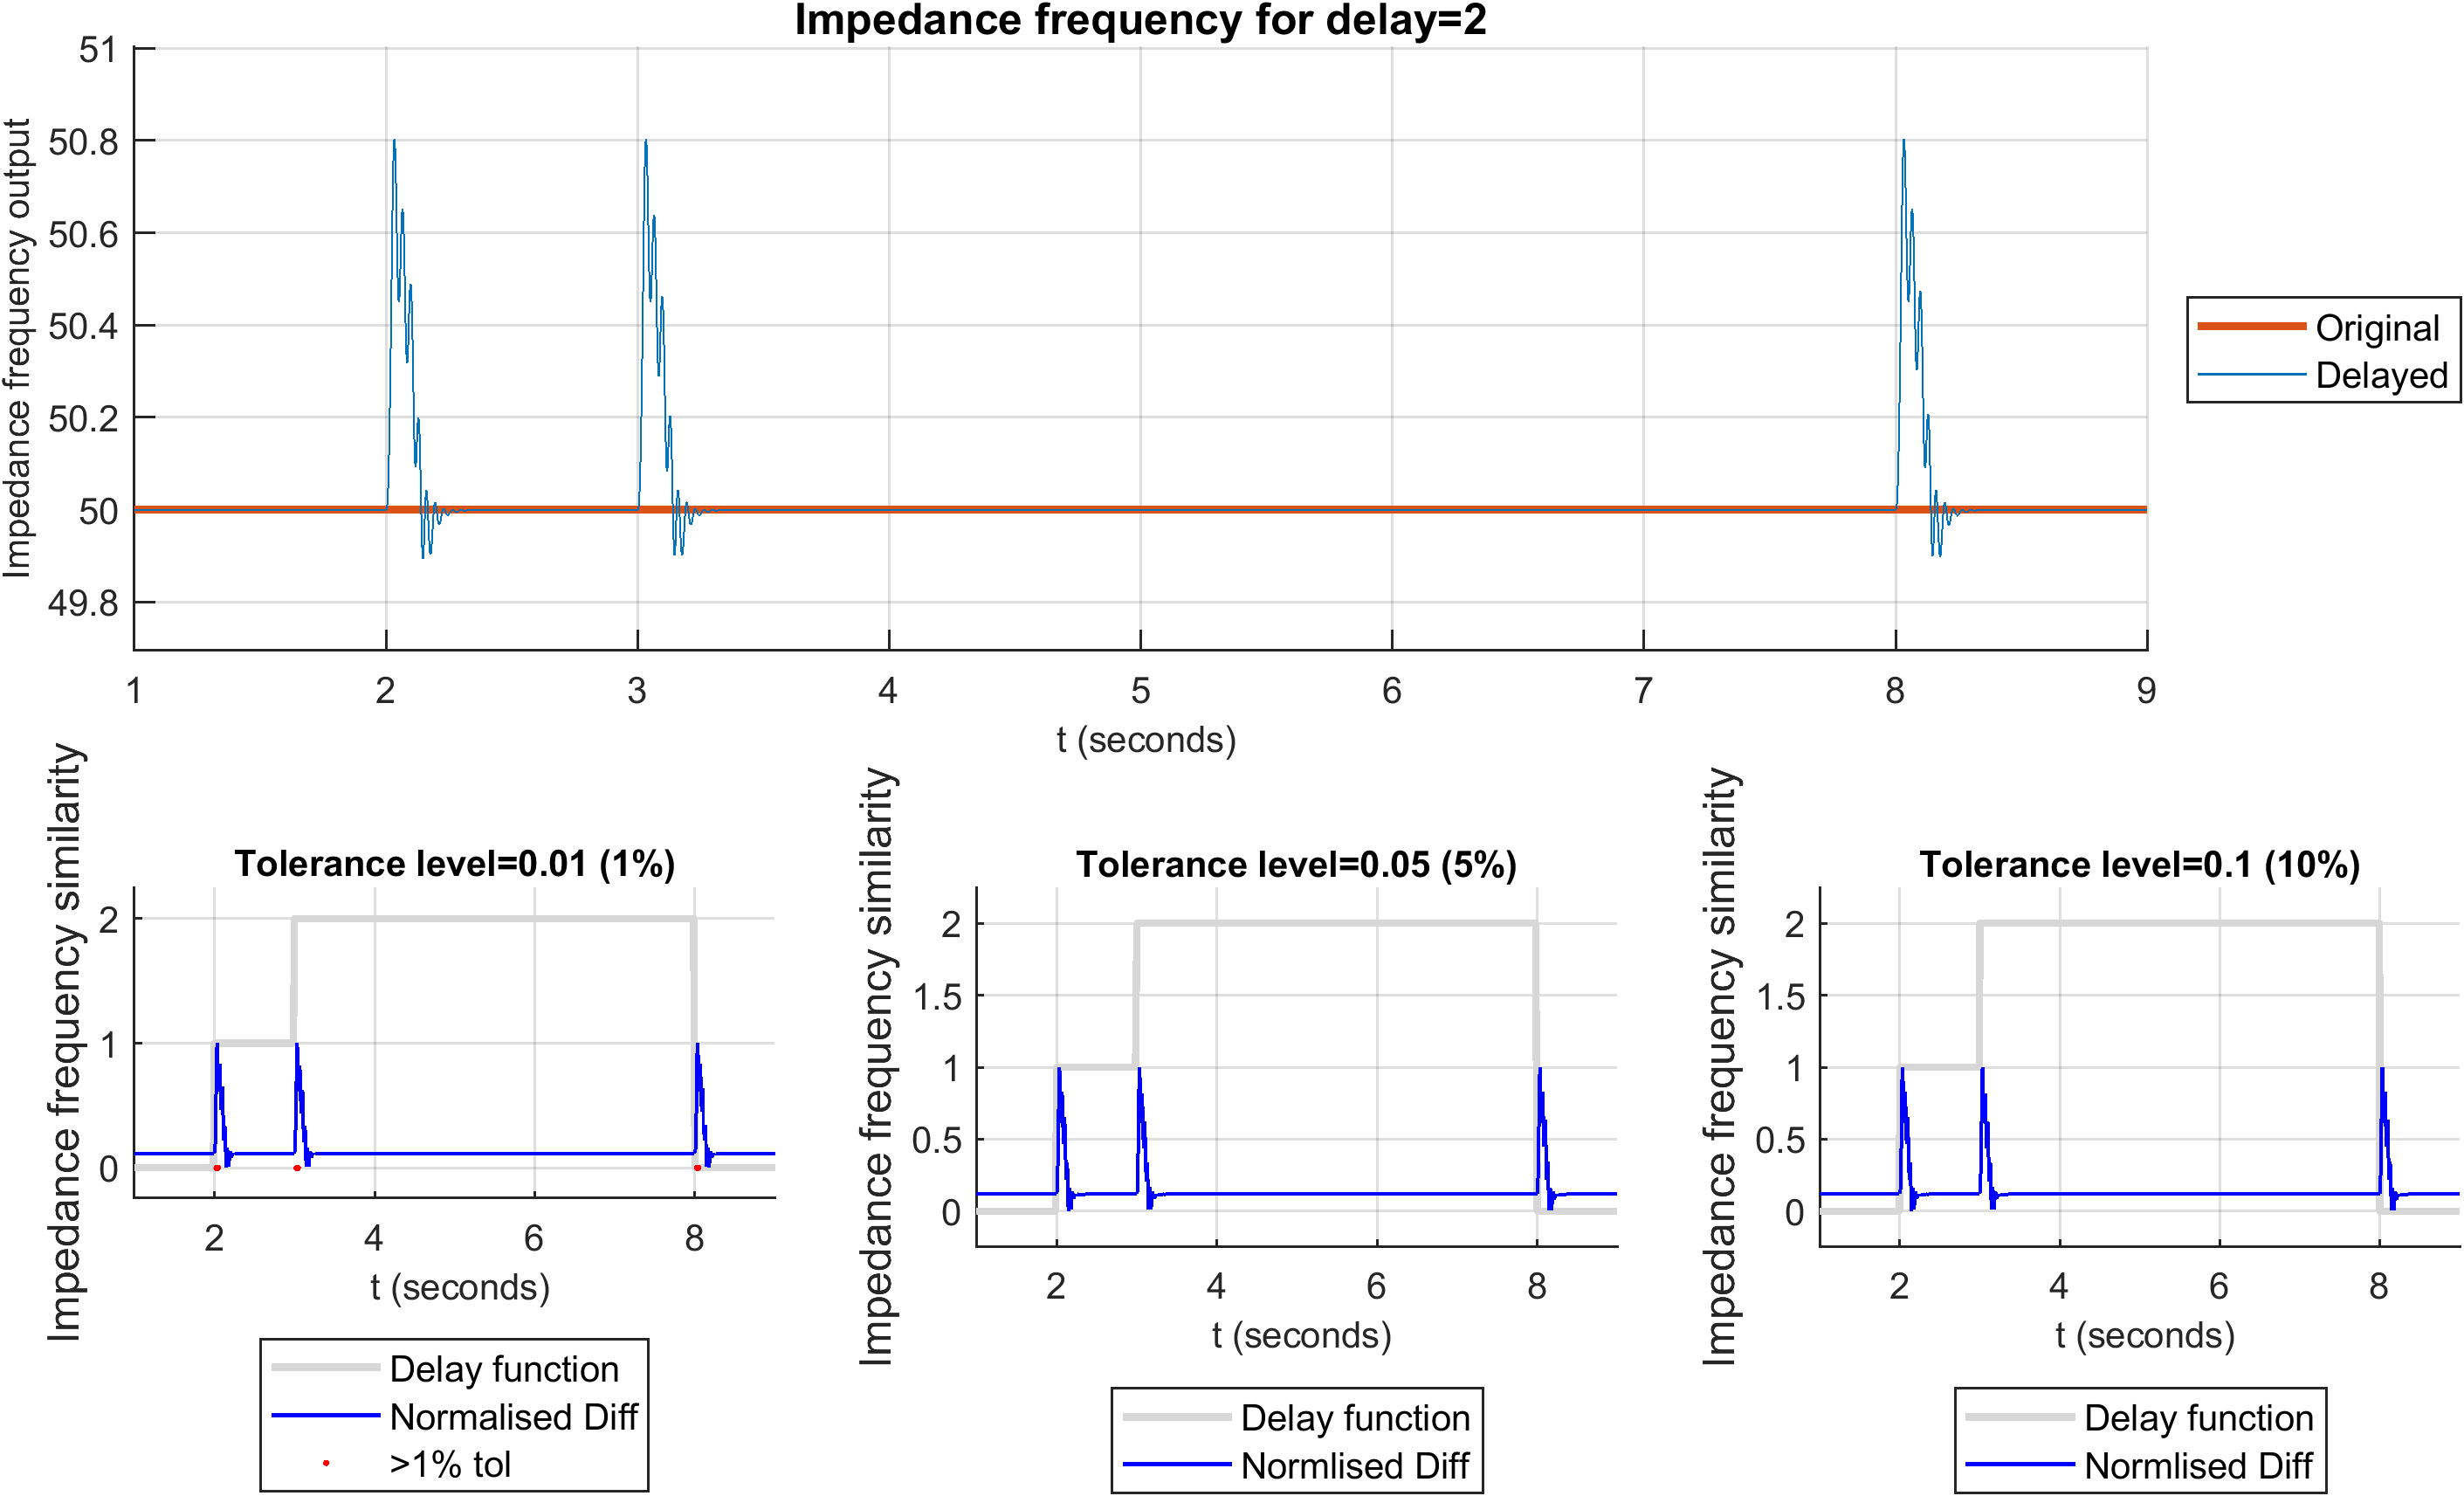
\includegraphics[width=0.95\textwidth]{PMUsim-figures/DelayOf_2/Step_iFrequency.png}    
    \label{fig:PMUsimStep_Two_Frequency}
\end{floatingfigure}
        \begin{small}
     \tcbox[size=small, standard jigsaw, opacityback=0, boxrule=0pt,halign=justify]{
     Comment on the figure:}{
     \begin{itemize}
         \item 
     \end{itemize} }
     \end{small}


\newpage \textbf{Results for Angle Output}


\begin{floatingfigure}[p]{\textwidth}
    \caption{Step-Wise Delay Angle Output for the Delay Level of Two}
    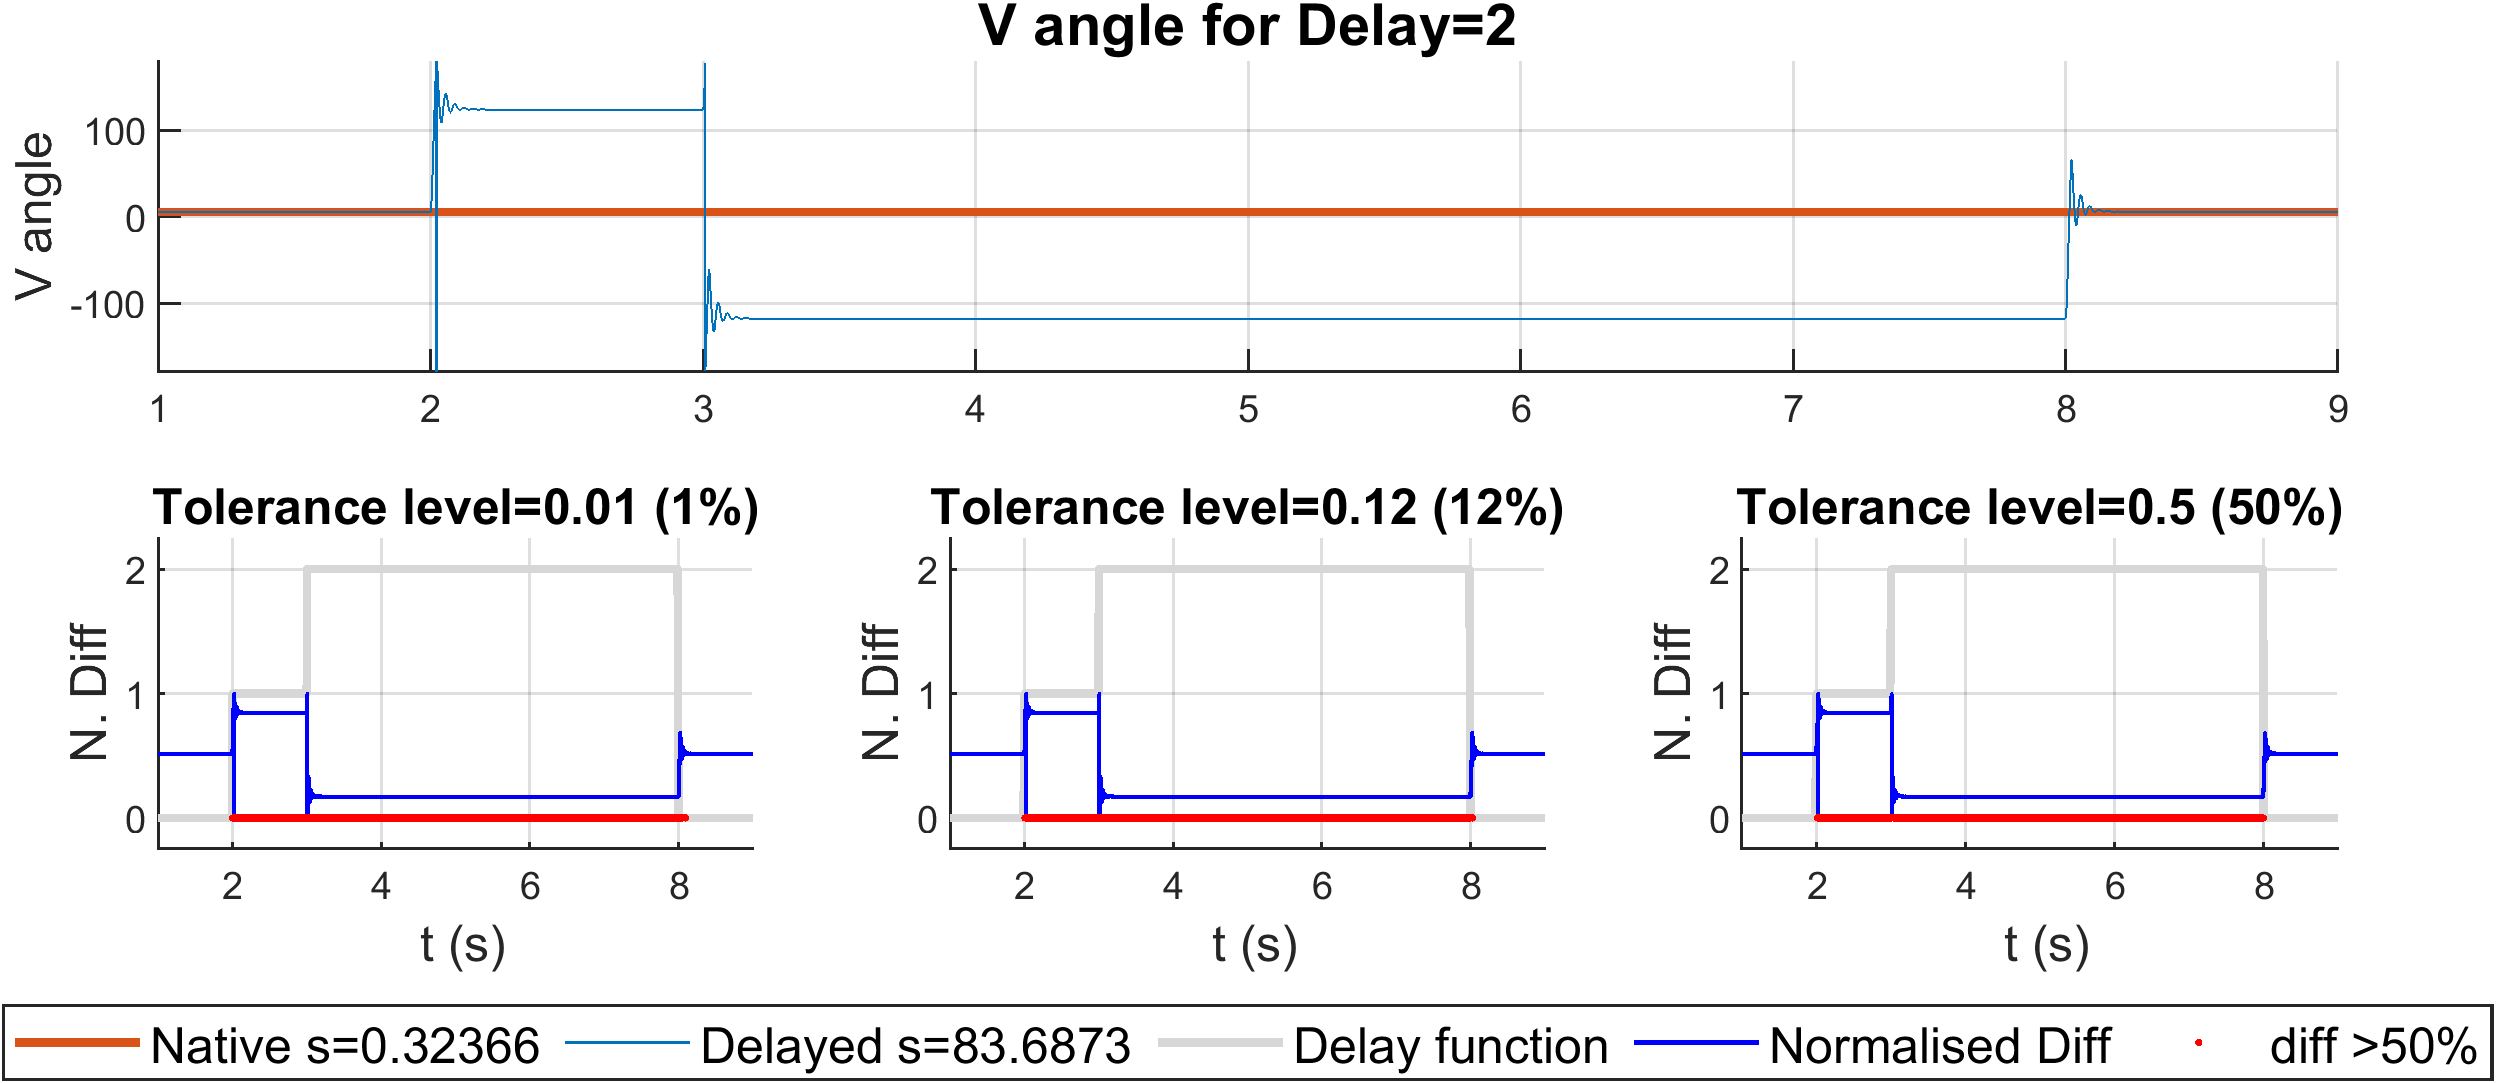
\includegraphics[width=0.95\textwidth]{PMUsim-figures/DelayOf_2/Step_vAngle.png}    
    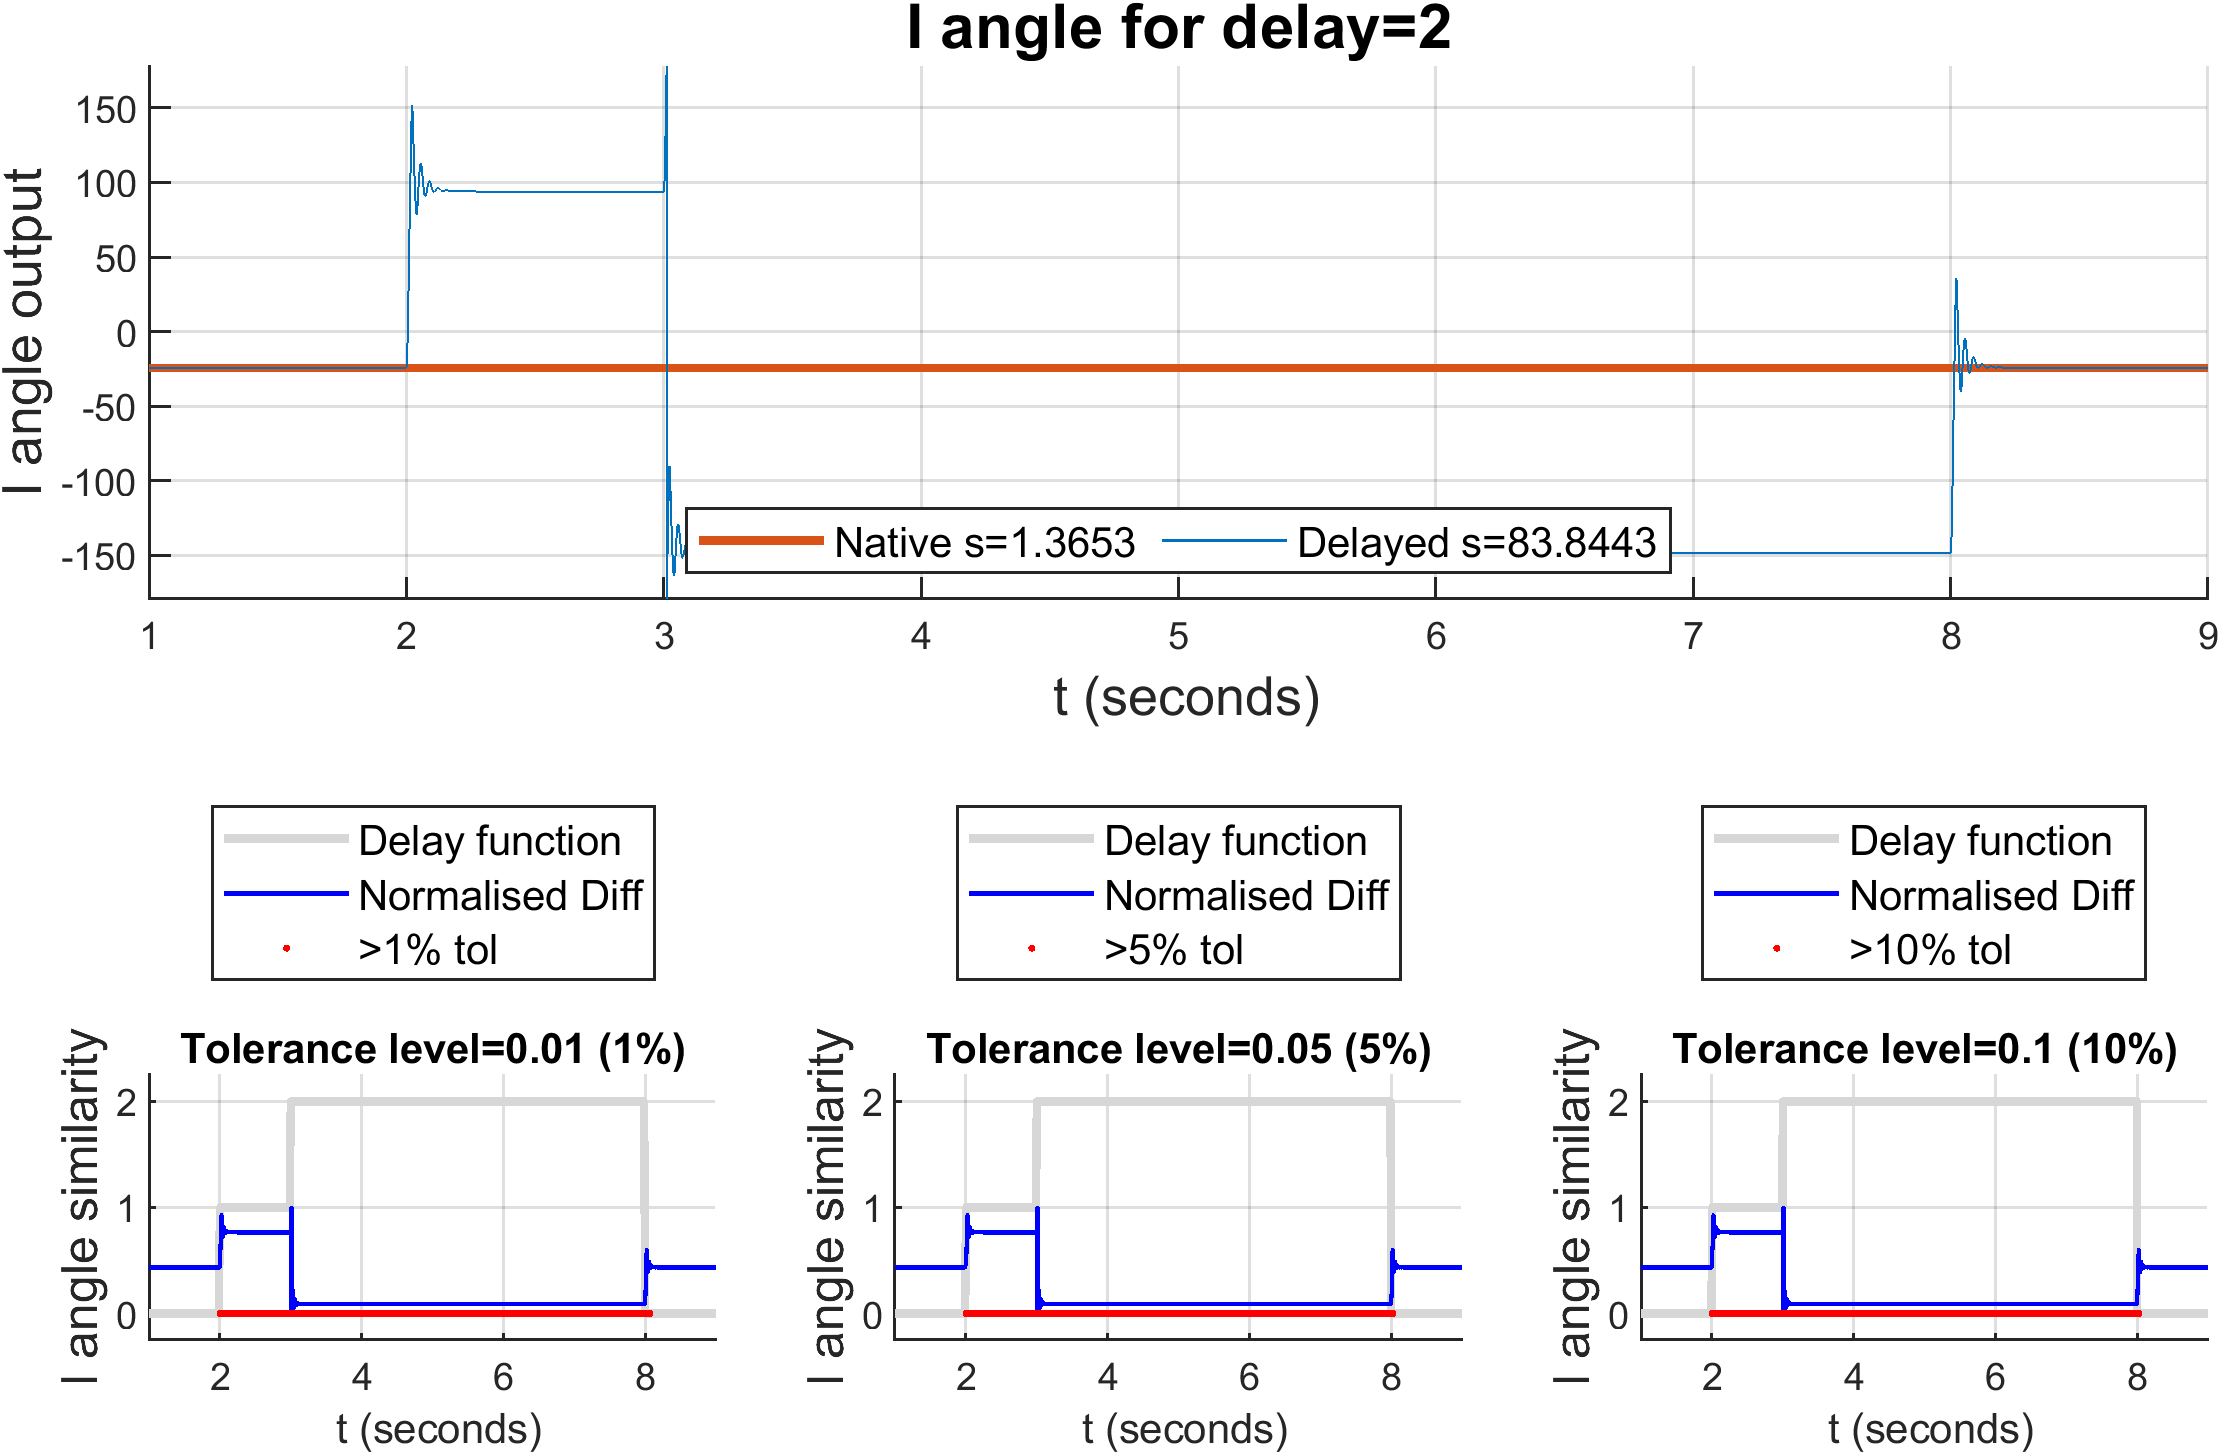
\includegraphics[width=0.95\textwidth]{PMUsim-figures/DelayOf_2/Step_iAngle.png}    
    \label{fig:PMUsimStep_Two_Angle}
\end{floatingfigure}
        \begin{small}
     \tcbox[size=small, standard jigsaw, opacityback=0, boxrule=0pt,halign=justify]{
     Comment on the figure:}{
     \begin{itemize}
         \item 
     \end{itemize} }
     \end{small}


\newpage \subsection{Delay Level of Three}
\textbf{Results for Magnitude Output}

\begin{floatingfigure}[p]{\textwidth}
    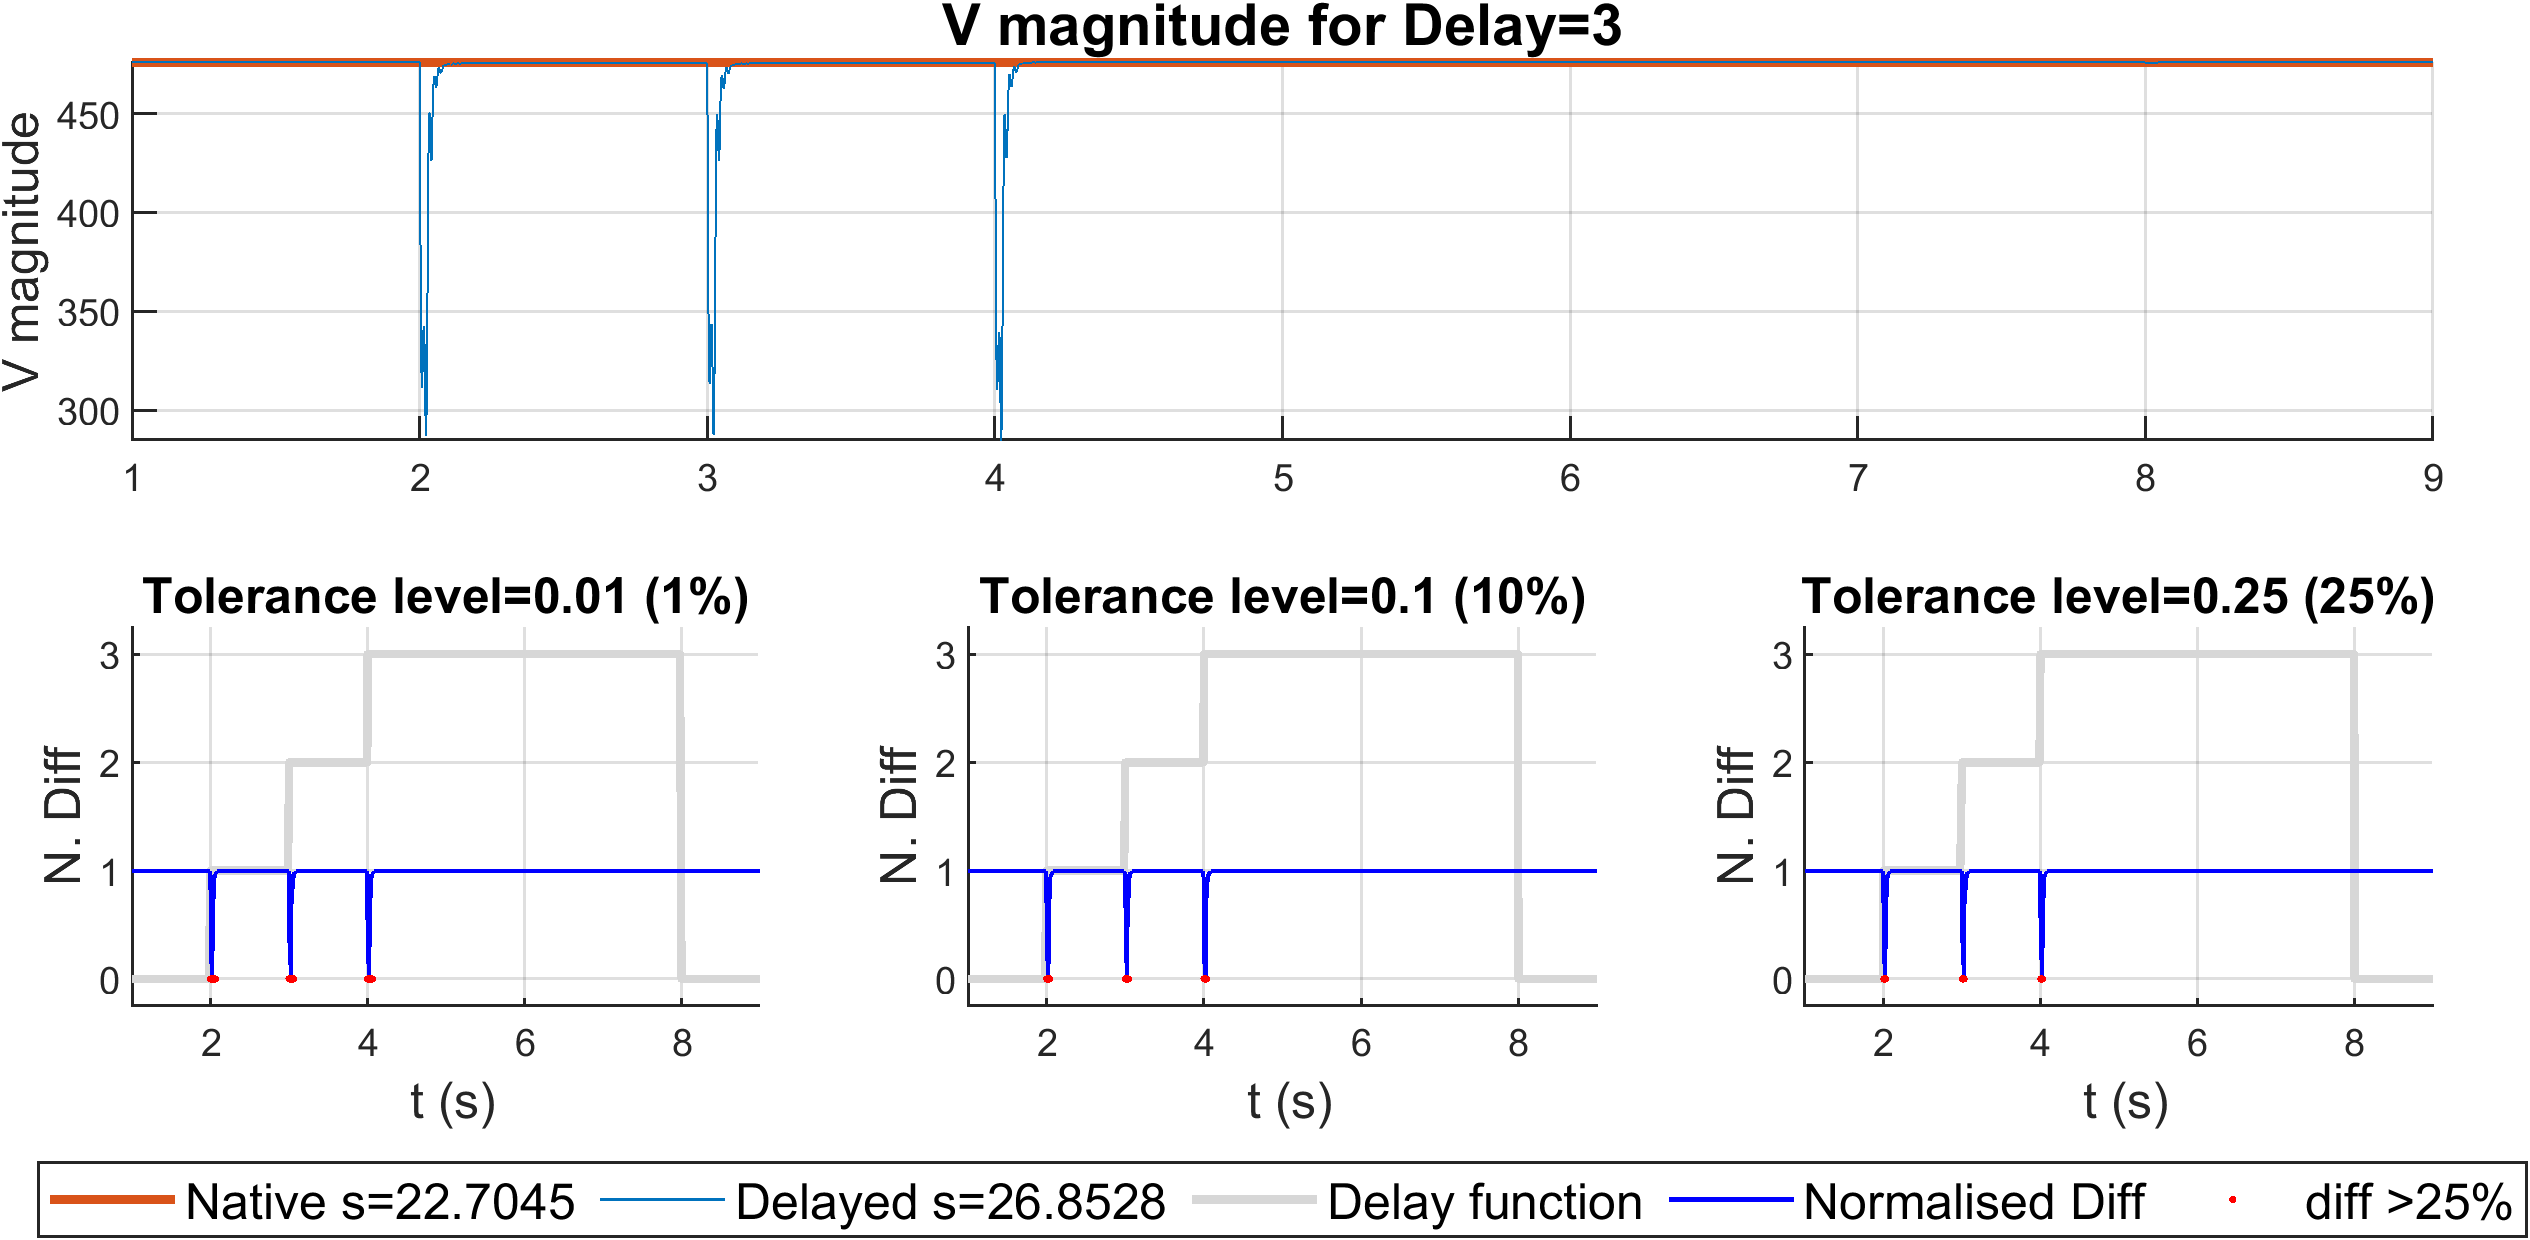
\includegraphics[width=0.95\textwidth]{PMUsim-figures/DelayOf_3/Step_vMagnitude.png}    
      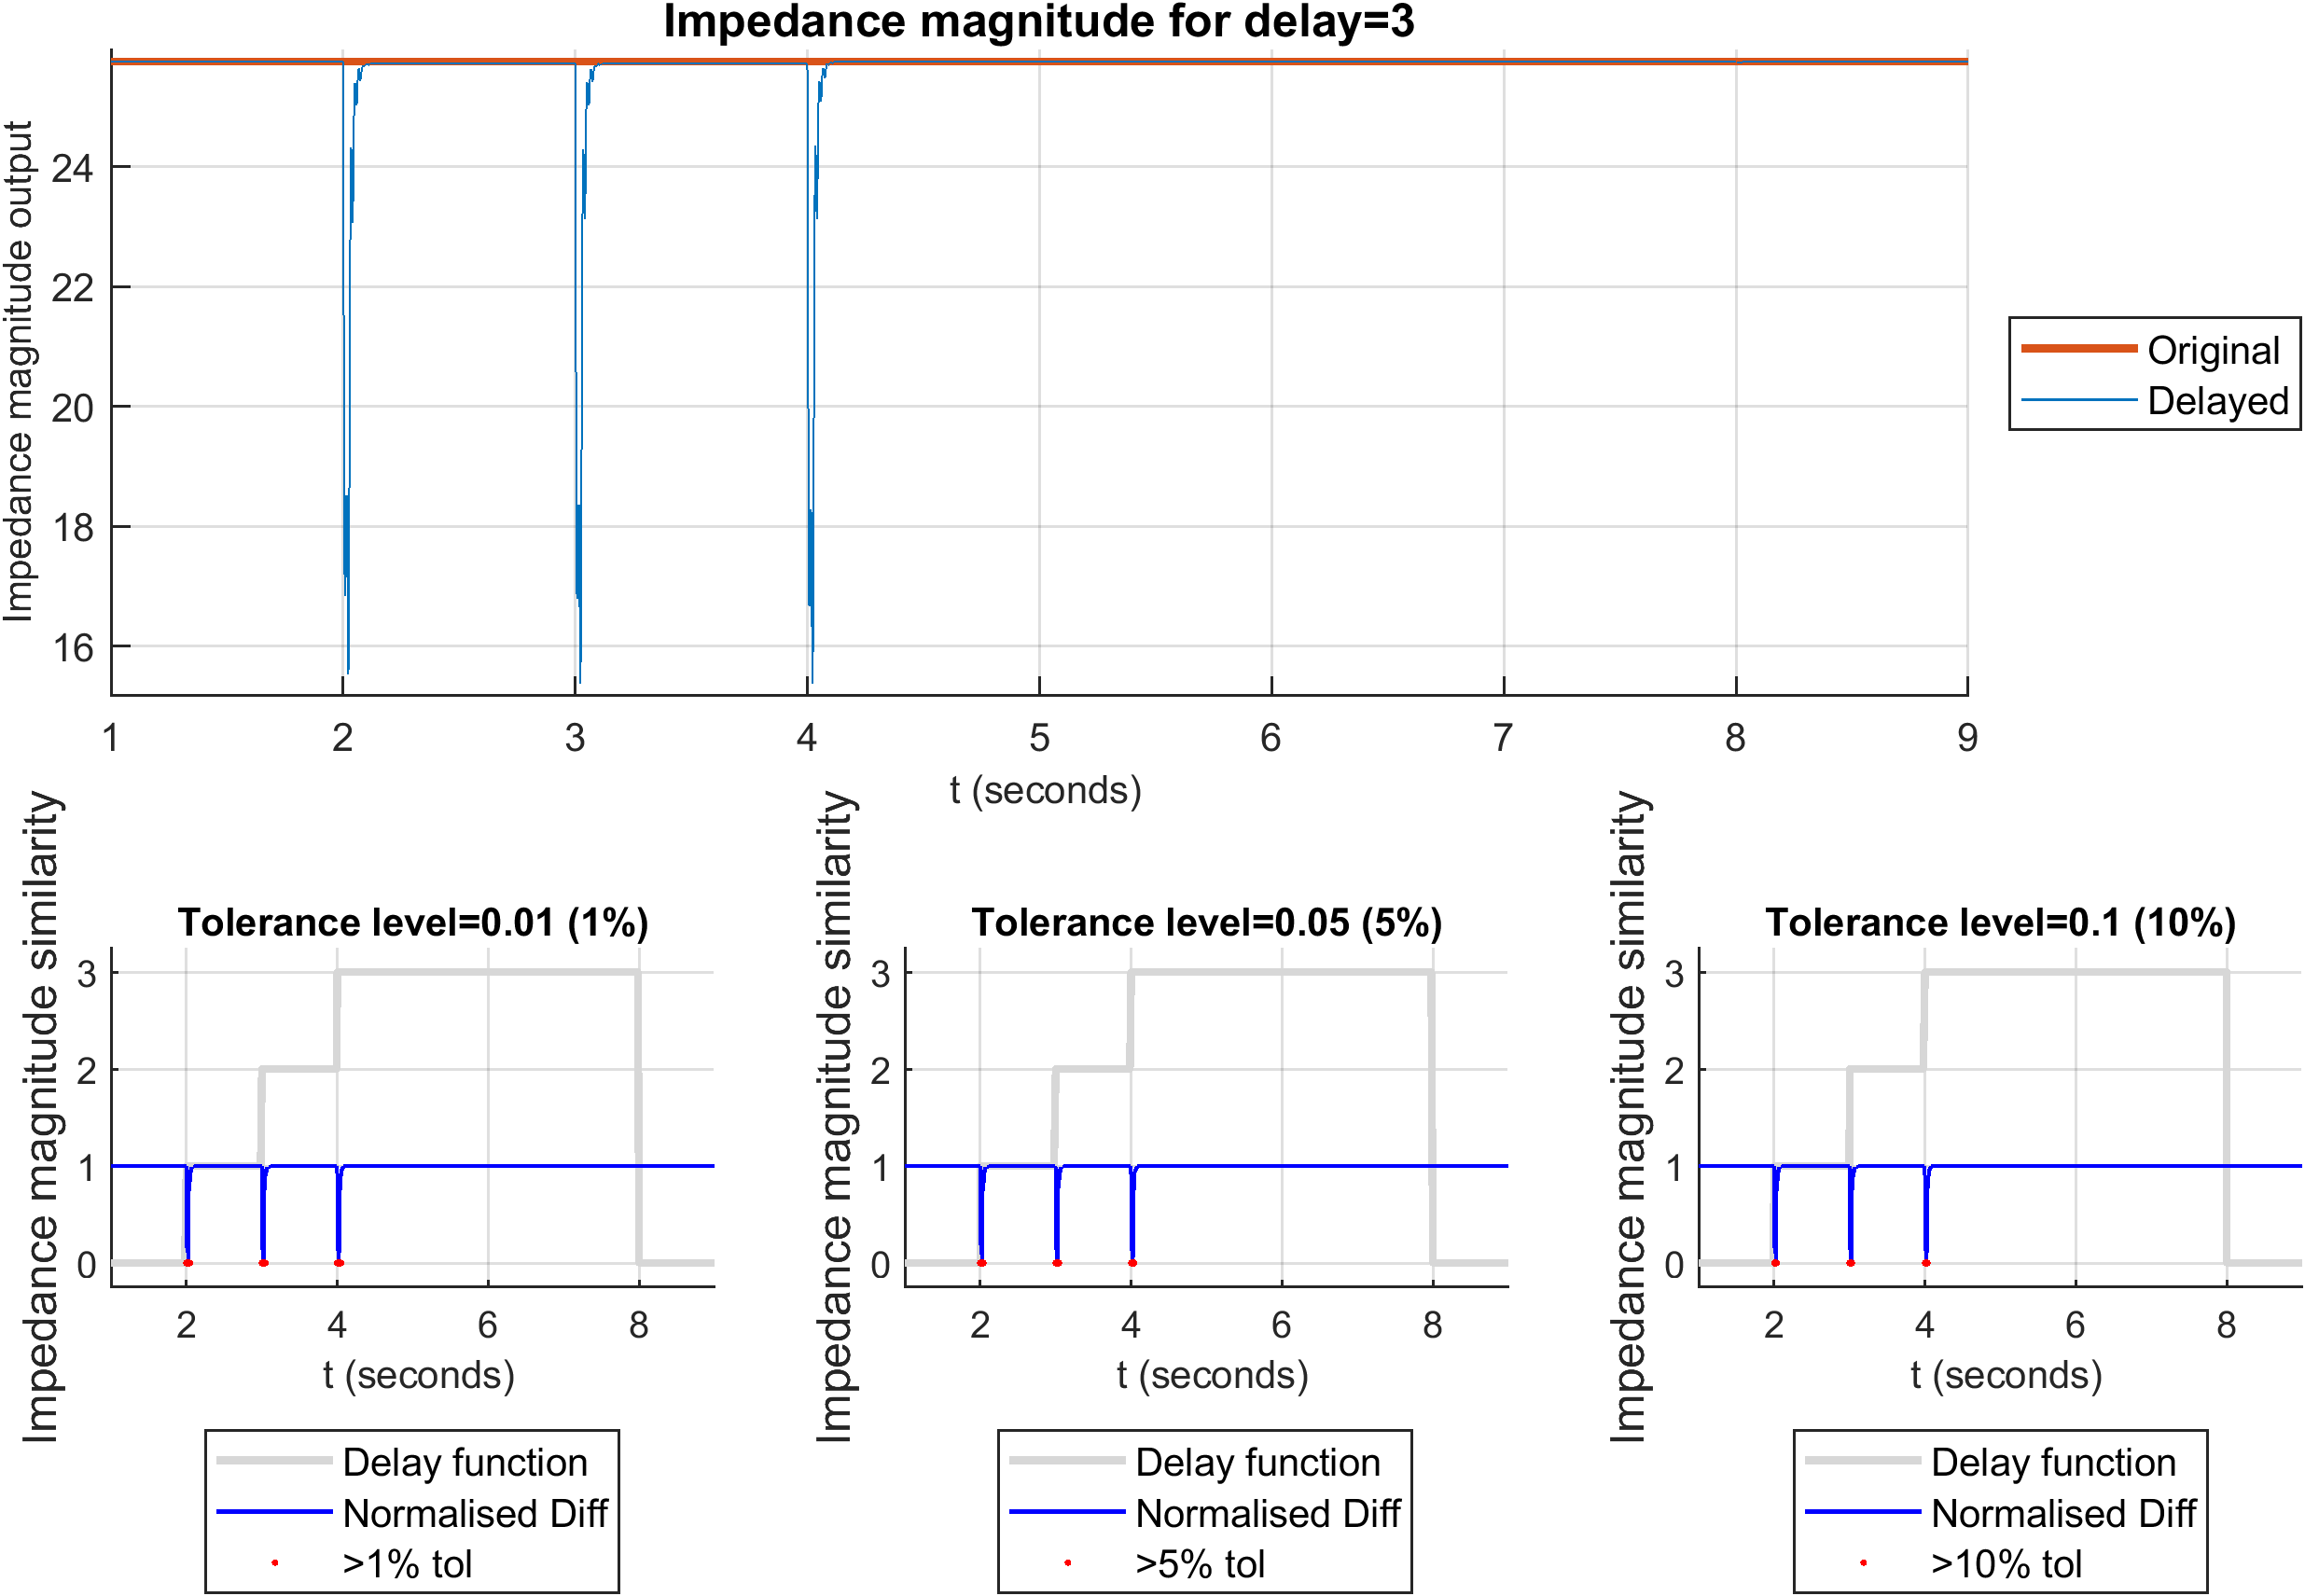
\includegraphics[width=0.95\textwidth]{PMUsim-figures/DelayOf_3/Step_iMagnitude.png}      
    \label{fig:PMUsimStep_Three_Magnitude}
    \caption{Step-Wise Delay Magnitude Output for the Delay Level of Three}
\end{floatingfigure}

    \begin{small}
     \tcbox[size=small, standard jigsaw, opacityback=0, boxrule=0pt,halign=justify]{
     Comment on the figure:}{
     \begin{itemize}
         \item 
     \end{itemize} }
     \end{small}

\newpage \textbf{Results for Frequency Output}


\begin{floatingfigure}[p]{\textwidth}
    \includegraphics[width=0.95\textwidth]{PMUsim-figures/DelayOf_3/Step_vFrequency.png}    
    \label{fig:PMUsimStep_Three_vFrequency}
    \includegraphics[width=0.95\textwidth]{PMUsim-figures/DelayOf_3/Step_iFrequency.png}    
    \label{fig:PMUsimStep_Three_Frequency}
    \caption{Step-Wise Delay Frequency Output for the Delay Level of Three}
\end{floatingfigure}

        \begin{small}
     \tcbox[size=small, standard jigsaw, opacityback=0, boxrule=0pt,halign=justify]{
     Comment on the figure:}{
     \begin{itemize}
         \item 
     \end{itemize} }
     \end{small}


\newpage \textbf{Results for Angle Output}


\begin{floatingfigure}[p]{\textwidth}
    \includegraphics[width=0.95\textwidth]{PMUsim-figures/DelayOf_3/Step_vAngle.png}    
    \includegraphics[width=0.95\textwidth]{PMUsim-figures/DelayOf_3/Step_iAngle.png}    
    \label{fig:PMUsimStep_Three_Angle}
    \caption{Step-Wise Delay Angle Output for the Delay Level of Three}
\end{floatingfigure}

        \begin{small}
     \tcbox[size=small, standard jigsaw, opacityback=0, boxrule=0pt,halign=justify]{
     Comment on the figure:}{
     \begin{itemize}
         \item 
     \end{itemize} }
     \end{small}

\newpage \subsection{Delay Level of Four}
\textbf{Results for Magnitude Output}

\begin{floatingfigure}[p]{\textwidth}
    \includegraphics[width=0.95\textwidth]{PMUsim-figures/DelayOf_4/Step_vMagnitude.png}    
      \includegraphics[width=0.95\textwidth]{PMUsim-figures/DelayOf_4/Step_iMagnitude.png}      
    \label{fig:PMUsimStep_Four_Magnitude}
    \caption{Step-Wise Delay Magnitude Output for the Delay Level of Four}
\end{floatingfigure}

    \begin{small}
     \tcbox[size=small, standard jigsaw, opacityback=0, boxrule=0pt,halign=justify]{
     Comment on the figure:}{
     \begin{itemize}
         \item 
     \end{itemize} }
     \end{small}

\newpage \textbf{Results for Frequency Output}


\begin{floatingfigure}[p]{\textwidth}
    \includegraphics[width=0.95\textwidth]{PMUsim-figures/DelayOf_4/Step_vFrequency.png}    
    \label{fig:PMUsimStep_Four_vFrequency}
    \includegraphics[width=0.95\textwidth]{PMUsim-figures/DelayOf_4/Step_iFrequency.png}    
    \label{fig:PMUsimStep_Four_Frequency}
    \caption{Step-Wise Delay Frequency Output for the Delay Level of Four}
\end{floatingfigure}

        \begin{small}
     \tcbox[size=small, standard jigsaw, opacityback=0, boxrule=0pt,halign=justify]{
     Comment on the figure:}{
     \begin{itemize}
         \item 
     \end{itemize} }
     \end{small}


\newpage \textbf{Results for Angle Output}


\begin{floatingfigure}[p]{\textwidth}
    \includegraphics[width=0.95\textwidth]{PMUsim-figures/DelayOf_4/Step_vAngle.png}    
    \includegraphics[width=0.95\textwidth]{PMUsim-figures/DelayOf_4/Step_iAngle.png}    
    \label{fig:PMUsimStep_Four_Angle}
    \caption{Step-Wise Delay Angle Output for the Delay Level of Four}
\end{floatingfigure}

        \begin{small}
     \tcbox[size=small, standard jigsaw, opacityback=0, boxrule=0pt,halign=justify]{
     Comment on the figure:}{
     \begin{itemize}
         \item 
     \end{itemize} }
     \end{small}

\newpage \subsection{Delay Level of Five}
\textbf{Results for Magnitude Output}

\begin{floatingfigure}[p]{\textwidth}
    \includegraphics[width=0.95\textwidth]{PMUsim-figures/DelayOf_5/Step_vMagnitude.png}    
      \includegraphics[width=0.95\textwidth]{PMUsim-figures/DelayOf_5/Step_iMagnitude.png}      
    \label{fig:PMUsimStep_Five_Magnitude}
    \caption{Step-Wise Delay Magnitude Output for the Delay Level of Five}
\end{floatingfigure}

    \begin{small}
     \tcbox[size=small, standard jigsaw, opacityback=0, boxrule=0pt,halign=justify]{
     Comment on the figure:}{
     \begin{itemize}
         \item 
     \end{itemize} }
     \end{small}

\newpage \textbf{Results for Frequency Output}


\begin{floatingfigure}[p]{\textwidth}
    \includegraphics[width=0.95\textwidth]{PMUsim-figures/DelayOf_5/Step_vFrequency.png}    
    \label{fig:PMUsimStep_Five_vFrequency}
    \includegraphics[width=0.95\textwidth]{PMUsim-figures/DelayOf_5/Step_iFrequency.png}    
    \label{fig:PMUsimStep_Five_Frequency}
    \caption{Step-Wise Delay Frequency Output for the Delay Level of Five}
\end{floatingfigure}

        \begin{small}
     \tcbox[size=small, standard jigsaw, opacityback=0, boxrule=0pt,halign=justify]{
     Comment on the figure:}{
     \begin{itemize}
         \item 
     \end{itemize} }
     \end{small}


\newpage \textbf{Results for Angle Output}


\begin{floatingfigure}[p]{\textwidth}
    \includegraphics[width=0.95\textwidth]{PMUsim-figures/DelayOf_5/Step_vAngle.png}    
    \includegraphics[width=0.95\textwidth]{PMUsim-figures/DelayOf_5/Step_iAngle.png}    
    \label{fig:PMUsimStep_Five_Angle}
    \caption{Step-Wise Delay Angle Output for the Delay Level of Five}
\end{floatingfigure}

        \begin{small}
     \tcbox[size=small, standard jigsaw, opacityback=0, boxrule=0pt,halign=justify]{
     Comment on the figure:}{
     \begin{itemize}
         \item 
     \end{itemize} }
     \end{small}

\newpage \subsection{Delay Level of Six}
\textbf{Results for Magnitude Output}

\begin{floatingfigure}[p]{\textwidth}
    \includegraphics[width=0.95\textwidth]{PMUsim-figures/DelayOf_6/Step_vMagnitude.png}    
      \includegraphics[width=0.95\textwidth]{PMUsim-figures/DelayOf_6/Step_iMagnitude.png}  
    \label{fig:PMUsimStep_Six_Magnitude}
    \caption{Step-Wise Delay Magnitude Output for the Delay Level of Six}
\end{floatingfigure}

    \begin{small}
     \tcbox[size=small, standard jigsaw, opacityback=0, boxrule=0pt,halign=justify]{
     Comment on the figure:}{
     \begin{itemize}
         \item 
     \end{itemize} }
     \end{small}

\newpage \textbf{Results for Frequency Output}


\begin{floatingfigure}[p]{\textwidth}
    \includegraphics[width=0.95\textwidth]{PMUsim-figures/DelayOf_6/Step_vFrequency.png}    
    \label{fig:PMUsimStep_Six_vFrequency}
    \includegraphics[width=0.95\textwidth]{PMUsim-figures/DelayOf_6/Step_iFrequency.png}    
    \label{fig:PMUsimStep_Six_Frequency}
    \caption{Step-Wise Delay Frequency Output for the Delay Level of Six}
\end{floatingfigure}

        \begin{small}
     \tcbox[size=small, standard jigsaw, opacityback=0, boxrule=0pt,halign=justify]{
     Comment on the figure:}{
     \begin{itemize}
         \item 
     \end{itemize} }
     \end{small}


\newpage \textbf{Results for Angle Output}


\begin{floatingfigure}[p]{\textwidth}
    \includegraphics[width=0.95\textwidth]{PMUsim-figures/DelayOf_6/Step_vAngle.png}    
    \includegraphics[width=0.95\textwidth]{PMUsim-figures/DelayOf_6/Step_iAngle.png}    
    \label{fig:PMUsimStep_Six_Angle}
    \caption{Step-Wise Delay Angle Output for the Delay Level of Six}
\end{floatingfigure}

        \begin{small}
     \tcbox[size=small, standard jigsaw, opacityback=0, boxrule=0pt,halign=justify]{
     Comment on the figure:}{
     \begin{itemize}
         \item 
     \end{itemize} }
     \end{small}
